\documentclass[11pt,openany,leqno]{book} % oneside twoside / report book / openany - bibl nie musi rozpoczynać się od nieparzystej
\usepackage[X2,T1]{fontenc}
\usepackage[utf8]{inputenc}
\usepackage{setspace}

\raggedbottom %usuwa przerwy między akapitami, spowodowane przez klasę book
\frenchspacing %usuwa podwójną przerwę po krpoce (zdaniu)

\usepackage{pdfpages}








\usepackage{graphicx}
%\usepackage{epic}
\usepackage{color}
\usepackage{amsmath}
\usepackage{bm}	% \boldsymbol
%\usepackage{amsbsy}	% \boldsymbol
\usepackage{amscd}	% diagramy
\usepackage{amsfonts}	% fonty
\usepackage{amssymb}	% dodatek math
\usepackage{amstext}	% \text
\usepackage{amsthm}
\usepackage{amsmath}
\usepackage{xfrac} %\sfrac{1}{2}
%\usepackage{nicefrac} %\nicefrac{1}{2}
\usepackage[normalem]{ulem}





\usepackage{longtable}
\usepackage{tabularx}
\renewcommand{\tabularxcolumn}[1]{m{#1}}
\newcolumntype{Y}{>{\centering\arraybackslash}X}
\newcolumntype{s}{>{\hsize=.8\hsize}X}
\renewcommand\arraystretch{1.2}
\usepackage{float} %umożliwia hard positioning (flaga: H)
\usepackage{supertabular}


\usepackage{array}
\usepackage{ragged2e}

%\newcolumntype{L}[1]{>{\RaggedRight\arraybackslash}m{#1}}
\newcolumntype{L}[1]{>{\RaggedRight\let\newline\arraybackslash}m{#1}}

\usepackage{adjustbox}




%Equation z marginesami
\usepackage{environ}
\makeatletter
\NewEnviron{widerequation}{%
	\begin{equation*}
	\sbox\z@{\let\label\@gobble$\displaystyle\BODY$}
	\makebox[\textwidth]{%
		\begin{minipage}{\dimexpr\wd\z@+3em}
		\vspace{-\baselineskip}
		\begin{equation*}
		\BODY
		\end{equation*}
		\end{minipage}%
	}
	\end{equation*}
}


\usepackage{emptypage}


\usepackage[protrusion=true,expansion=true]{microtype}

\usepackage{multicol}


% Different font in captions
\newcommand{\captionfonts}{\small} %wydaje sie, ze nie dziala
\usepackage[font={small},singlelinecheck=false]{caption}



%---------------------------------------------------------
\usepackage{xcolor}
\usepackage{stmaryrd} %dla podwójnego nawiasu w mathmode (przypisanie interpretacji formule/zdaniu) \llbracket \rrbracket
\usepackage{textcomp} %dla podwójnego nawiasu w textmode (przypisanie interpretacji formule/zdaniu) \textlbrackdbl \textrbrackdbl
\usepackage{tikz-cd}
\usetikzlibrary{babel}
%\usetikzlibrary{shapes.geometric}
\usepackage[title]{appendix}


\usepackage[hyphens,spaces,obeyspaces]{url}
\usepackage{hyperref} %to nowsza wersja pakietu url, lepsza m.in. robie linki hyperref
\hypersetup{colorlinks=true, linkcolor=black, citecolor=black, urlcolor=black, breaklinks=true, linktocpage}  %to sprawia że nie widać w pdfie aktywnych linków (od GM)
\urlstyle{rm}
%\usepackage[hyphens]{url}
%\PassOptionsToPackage{hyphens}{url}%
%\RequirePackage[hyphens]{url}



%--------------------------------------------------------------------------------




\usepackage[russian,polutonikogreek,greek,german,english,polish]{babel}
\usepackage{textgreek}

\usepackage{geometry}
\geometry{verbose,paperwidth=145mm,paperheight=205mm,landscape=false,
twoside,top=25mm,bottom=20mm,left=23mm,right=23mm,headheight=14pt}

%-----spady---------
%\usepackage[cam,a4,center]{crop}
%\usepackage[width=151mm,height=211mm,center,cam,noinfo]{crop} % konsultuj z dokumentacją
\usepackage[width=151mm,height=211mm,center,noinfo]{crop} % bex lini citęcia, konsultuj z dokumentacją

\hyphenation{pseudo-recursive pseudo-recursiveness pseudorecur-siveness pseudo-recursion}
\hyphenation{var-iety var-ieties}
\hyphenation{Tisch-ner Tisch-ner-a}
\hyphenation{Sie-ro-to-wicz}
\hyphenation{Nord-haus}
\hyphenation{Flei-schacker}
\hyphenation{Fuku-yama}
\hyphenation{Be-cke-ra Be-cker}
\hyphenation{Schwei-tze-ra}
\hyphenation{me-ta-e-ko-no-mi-czne}
\hyphenation{McCloskey}





%\usepackage{paralist}     %odstępy w listach
%  \let\itemize\compactitem
%  \let\enditemize\endcompactitem
%  \let\enumerate\compactenum
%  \let\endenumerate\endcompactenum
%  \let\description\compactdesc
%  \let\enddescription\endcompactdesc
%  \pltopsep=\medskipamount
%  \plitemsep=1pt
%  \plparsep=1pt

\usepackage{enumitem}
\setlist{noitemsep} % lub \setlist{nosep}


%%lamza

\setlistdepth{8}
\newlist{longitemize}{itemize}{8}
\setlist[longitemize,1]{label=$\bullet$}
\setlist[longitemize,2]{label=$\circ$}
\setlist[longitemize,3]{label=$\ast$}
\setlist[longitemize,4]{label=$\bullet$}
\setlist[longitemize,5]{label=$\circ$}
\setlist[longitemize,6]{label=$\ast$}
\setlist[longitemize,7]{label=$\bullet$}
\setlist[longitemize,8]{label=$\bullet$}

\usepackage{scrextend}

%%%%liana
%\usepackage{mdframed} %sprawdzić, czy gdzieś nie szkodzi
%\newtheoremstyle{sltheorem}
%{0pt}                % Space above
%{1em}                % Space below
%{\small\mdseries}        % Theorem body font % (default is "\upshape")
%{}                % Indent amount
%{\itshape}       % Theorem head font % (default is \mdseries)
%{.}               % Punctuation after theorem head % default: no punctuation
%{ }               % Space after theorem head
%{}                % Theorem head spec
%\theoremstyle{sltheorem}
%\newtheorem{uwaga}{Uwaga}
%\surroundwithmdframed[linewidth=1pt,
%linecolor=black,
%bottomline=false,topline=false,rightline=false,
%innerrightmargin=0pt,innertopmargin=0pt,innerbottommargin=0pt,
%%outerrightmargin=0pt,outertopmargin=0pt,outerbottommargin=0pt,
%innerleftmargin=.5em,% Distance between vertical rule & proof content
%skipabove=1em,splittopskip=0pt,splitbottomskip=0pt%
%]{uwaga}



%------------------------- MyriadPro ------------------------------------
\usepackage{textcomp}
%\usepackage{Myriad}
% lcdf-typetools glyphtounicode.tex, Version 2.95
% Contents: Glyph mapping information for pdftex, used for PDF searching
% Generated from:
% - glyphlist.txt, Version 2.0
% - texglyphlist.txt, Version 2.95
% - texglyphlist-g2u.txt, Version 2.95
\pdfglyphtounicode{A}{0041}
\pdfglyphtounicode{AE}{00C6}
\pdfglyphtounicode{AEacute}{01FC}
\pdfglyphtounicode{AEmacron}{01E2}
\pdfglyphtounicode{AEsmall}{00E6}
\pdfglyphtounicode{Aacute}{00C1}
\pdfglyphtounicode{Aacutesmall}{00E1}
\pdfglyphtounicode{Abreve}{0102}
\pdfglyphtounicode{Abreveacute}{1EAE}
\pdfglyphtounicode{Abrevecyrillic}{04D0}
\pdfglyphtounicode{Abrevedotbelow}{1EB6}
\pdfglyphtounicode{Abrevegrave}{1EB0}
\pdfglyphtounicode{Abrevehookabove}{1EB2}
\pdfglyphtounicode{Abrevetilde}{1EB4}
\pdfglyphtounicode{Acaron}{01CD}
\pdfglyphtounicode{Acircle}{24B6}
\pdfglyphtounicode{Acircumflex}{00C2}
\pdfglyphtounicode{Acircumflexacute}{1EA4}
\pdfglyphtounicode{Acircumflexdotbelow}{1EAC}
\pdfglyphtounicode{Acircumflexgrave}{1EA6}
\pdfglyphtounicode{Acircumflexhookabove}{1EA8}
\pdfglyphtounicode{Acircumflexsmall}{00E2}
\pdfglyphtounicode{Acircumflextilde}{1EAA}
\pdfglyphtounicode{Acute}{00B4}
\pdfglyphtounicode{Acutesmall}{00B4}
\pdfglyphtounicode{Acyrillic}{0410}
\pdfglyphtounicode{Adblgrave}{0200}
\pdfglyphtounicode{Adieresis}{00C4}
\pdfglyphtounicode{Adieresiscyrillic}{04D2}
\pdfglyphtounicode{Adieresismacron}{01DE}
\pdfglyphtounicode{Adieresissmall}{00E4}
\pdfglyphtounicode{Adotbelow}{1EA0}
\pdfglyphtounicode{Adotmacron}{01E0}
\pdfglyphtounicode{Agrave}{00C0}
\pdfglyphtounicode{Agravesmall}{00E0}
\pdfglyphtounicode{Ahookabove}{1EA2}
\pdfglyphtounicode{Aiecyrillic}{04D4}
\pdfglyphtounicode{Ainvertedbreve}{0202}
\pdfglyphtounicode{Alpha}{0391}
\pdfglyphtounicode{Alphatonos}{0386}
\pdfglyphtounicode{Amacron}{0100}
\pdfglyphtounicode{Amonospace}{FF21}
\pdfglyphtounicode{Aogonek}{0104}
\pdfglyphtounicode{Aring}{00C5}
\pdfglyphtounicode{Aringacute}{01FA}
\pdfglyphtounicode{Aringbelow}{1E00}
\pdfglyphtounicode{Aringsmall}{00E5}
\pdfglyphtounicode{Asmall}{0061}
\pdfglyphtounicode{Atilde}{00C3}
\pdfglyphtounicode{Atildesmall}{00E3}
\pdfglyphtounicode{Aybarmenian}{0531}
\pdfglyphtounicode{B}{0042}
\pdfglyphtounicode{Bcircle}{24B7}
\pdfglyphtounicode{Bdotaccent}{1E02}
\pdfglyphtounicode{Bdotbelow}{1E04}
\pdfglyphtounicode{Becyrillic}{0411}
\pdfglyphtounicode{Benarmenian}{0532}
\pdfglyphtounicode{Beta}{0392}
\pdfglyphtounicode{Bhook}{0181}
\pdfglyphtounicode{Blinebelow}{1E06}
\pdfglyphtounicode{Bmonospace}{FF22}
\pdfglyphtounicode{Brevesmall}{02D8}
\pdfglyphtounicode{Bsmall}{0062}
\pdfglyphtounicode{Btopbar}{0182}
\pdfglyphtounicode{C}{0043}
\pdfglyphtounicode{Caarmenian}{053E}
\pdfglyphtounicode{Cacute}{0106}
\pdfglyphtounicode{Caron}{02C7}
\pdfglyphtounicode{Caronsmall}{02C7}
\pdfglyphtounicode{Ccaron}{010C}
\pdfglyphtounicode{Ccedilla}{00C7}
\pdfglyphtounicode{Ccedillaacute}{1E08}
\pdfglyphtounicode{Ccedillasmall}{00E7}
\pdfglyphtounicode{Ccircle}{24B8}
\pdfglyphtounicode{Ccircumflex}{0108}
\pdfglyphtounicode{Cdot}{010A}
\pdfglyphtounicode{Cdotaccent}{010A}
\pdfglyphtounicode{Cedillasmall}{00B8}
\pdfglyphtounicode{Chaarmenian}{0549}
\pdfglyphtounicode{Cheabkhasiancyrillic}{04BC}
\pdfglyphtounicode{Checyrillic}{0427}
\pdfglyphtounicode{Chedescenderabkhasiancyrillic}{04BE}
\pdfglyphtounicode{Chedescendercyrillic}{04B6}
\pdfglyphtounicode{Chedieresiscyrillic}{04F4}
\pdfglyphtounicode{Cheharmenian}{0543}
\pdfglyphtounicode{Chekhakassiancyrillic}{04CB}
\pdfglyphtounicode{Cheverticalstrokecyrillic}{04B8}
\pdfglyphtounicode{Chi}{03A7}
\pdfglyphtounicode{Chook}{0187}
\pdfglyphtounicode{Circumflexsmall}{02C6}
\pdfglyphtounicode{Cmonospace}{FF23}
\pdfglyphtounicode{Coarmenian}{0551}
\pdfglyphtounicode{Csmall}{0063}
\pdfglyphtounicode{D}{0044}
\pdfglyphtounicode{DZ}{01F1}
\pdfglyphtounicode{DZcaron}{01C4}
\pdfglyphtounicode{Daarmenian}{0534}
\pdfglyphtounicode{Dafrican}{0189}
\pdfglyphtounicode{Dbar}{0110}
\pdfglyphtounicode{Dcaron}{010E}
\pdfglyphtounicode{Dcedilla}{1E10}
\pdfglyphtounicode{Dcircle}{24B9}
\pdfglyphtounicode{Dcircumflexbelow}{1E12}
\pdfglyphtounicode{Dcroat}{0110}
\pdfglyphtounicode{Ddotaccent}{1E0A}
\pdfglyphtounicode{Ddotbelow}{1E0C}
\pdfglyphtounicode{Decyrillic}{0414}
\pdfglyphtounicode{Deicoptic}{03EE}
\pdfglyphtounicode{Delta}{2206}
\pdfglyphtounicode{Deltagreek}{0394}
\pdfglyphtounicode{Dhook}{018A}
\pdfglyphtounicode{Dieresis}{00A8}
\pdfglyphtounicode{DieresisAcute}{F6CC}
\pdfglyphtounicode{DieresisGrave}{F6CD}
\pdfglyphtounicode{Dieresissmall}{00A8}
\pdfglyphtounicode{Digamma}{D875 DFCB}
\pdfglyphtounicode{Digammagreek}{03DC}
\pdfglyphtounicode{Djecyrillic}{0402}
\pdfglyphtounicode{Dlinebelow}{1E0E}
\pdfglyphtounicode{Dmonospace}{FF24}
\pdfglyphtounicode{Dotaccentsmall}{02D9}
\pdfglyphtounicode{Dslash}{0110}
\pdfglyphtounicode{Dsmall}{0064}
\pdfglyphtounicode{Dtopbar}{018B}
\pdfglyphtounicode{Dz}{01F2}
\pdfglyphtounicode{Dzcaron}{01C5}
\pdfglyphtounicode{Dzeabkhasiancyrillic}{04E0}
\pdfglyphtounicode{Dzecyrillic}{0405}
\pdfglyphtounicode{Dzhecyrillic}{040F}
\pdfglyphtounicode{E}{0045}
\pdfglyphtounicode{Eacute}{00C9}
\pdfglyphtounicode{Eacutesmall}{00E9}
\pdfglyphtounicode{Ebreve}{0114}
\pdfglyphtounicode{Ecaron}{011A}
\pdfglyphtounicode{Ecedillabreve}{1E1C}
\pdfglyphtounicode{Echarmenian}{0535}
\pdfglyphtounicode{Ecircle}{24BA}
\pdfglyphtounicode{Ecircumflex}{00CA}
\pdfglyphtounicode{Ecircumflexacute}{1EBE}
\pdfglyphtounicode{Ecircumflexbelow}{1E18}
\pdfglyphtounicode{Ecircumflexdotbelow}{1EC6}
\pdfglyphtounicode{Ecircumflexgrave}{1EC0}
\pdfglyphtounicode{Ecircumflexhookabove}{1EC2}
\pdfglyphtounicode{Ecircumflexsmall}{00EA}
\pdfglyphtounicode{Ecircumflextilde}{1EC4}
\pdfglyphtounicode{Ecyrillic}{0404}
\pdfglyphtounicode{Edblgrave}{0204}
\pdfglyphtounicode{Edieresis}{00CB}
\pdfglyphtounicode{Edieresissmall}{00EB}
\pdfglyphtounicode{Edot}{0116}
\pdfglyphtounicode{Edotaccent}{0116}
\pdfglyphtounicode{Edotbelow}{1EB8}
\pdfglyphtounicode{Efcyrillic}{0424}
\pdfglyphtounicode{Egrave}{00C8}
\pdfglyphtounicode{Egravesmall}{00E8}
\pdfglyphtounicode{Eharmenian}{0537}
\pdfglyphtounicode{Ehookabove}{1EBA}
\pdfglyphtounicode{Eightroman}{2167}
\pdfglyphtounicode{Einvertedbreve}{0206}
\pdfglyphtounicode{Eiotifiedcyrillic}{0464}
\pdfglyphtounicode{Elcyrillic}{041B}
\pdfglyphtounicode{Elevenroman}{216A}
\pdfglyphtounicode{Emacron}{0112}
\pdfglyphtounicode{Emacronacute}{1E16}
\pdfglyphtounicode{Emacrongrave}{1E14}
\pdfglyphtounicode{Emcyrillic}{041C}
\pdfglyphtounicode{Emonospace}{FF25}
\pdfglyphtounicode{Encyrillic}{041D}
\pdfglyphtounicode{Endescendercyrillic}{04A2}
\pdfglyphtounicode{Eng}{014A}
\pdfglyphtounicode{Enghecyrillic}{04A4}
\pdfglyphtounicode{Enhookcyrillic}{04C7}
\pdfglyphtounicode{Eogonek}{0118}
\pdfglyphtounicode{Eopen}{0190}
\pdfglyphtounicode{Epsilon}{0395}
\pdfglyphtounicode{Epsilontonos}{0388}
\pdfglyphtounicode{Ercyrillic}{0420}
\pdfglyphtounicode{Ereversed}{018E}
\pdfglyphtounicode{Ereversedcyrillic}{042D}
\pdfglyphtounicode{Escyrillic}{0421}
\pdfglyphtounicode{Esdescendercyrillic}{04AA}
\pdfglyphtounicode{Esh}{01A9}
\pdfglyphtounicode{Esmall}{0065}
\pdfglyphtounicode{Eta}{0397}
\pdfglyphtounicode{Etarmenian}{0538}
\pdfglyphtounicode{Etatonos}{0389}
\pdfglyphtounicode{Eth}{00D0}
\pdfglyphtounicode{Ethsmall}{00F0}
\pdfglyphtounicode{Etilde}{1EBC}
\pdfglyphtounicode{Etildebelow}{1E1A}
\pdfglyphtounicode{Euro}{20AC}
\pdfglyphtounicode{Ezh}{01B7}
\pdfglyphtounicode{Ezhcaron}{01EE}
\pdfglyphtounicode{Ezhreversed}{01B8}
\pdfglyphtounicode{F}{0046}
\pdfglyphtounicode{FFIsmall}{0066 0066 0069}
\pdfglyphtounicode{FFLsmall}{0066 0066 006C}
\pdfglyphtounicode{FFsmall}{0066 0066}
\pdfglyphtounicode{FIsmall}{0066 0069}
\pdfglyphtounicode{FLsmall}{0066 006C}
\pdfglyphtounicode{Fcircle}{24BB}
\pdfglyphtounicode{Fdotaccent}{1E1E}
\pdfglyphtounicode{Feharmenian}{0556}
\pdfglyphtounicode{Feicoptic}{03E4}
\pdfglyphtounicode{Fhook}{0191}
\pdfglyphtounicode{Finv}{2132}
\pdfglyphtounicode{Fitacyrillic}{0472}
\pdfglyphtounicode{Fiveroman}{2164}
\pdfglyphtounicode{Fmonospace}{FF26}
\pdfglyphtounicode{Fourroman}{2163}
\pdfglyphtounicode{Fsmall}{0066}
\pdfglyphtounicode{G}{0047}
\pdfglyphtounicode{GBsquare}{3387}
\pdfglyphtounicode{Gacute}{01F4}
\pdfglyphtounicode{Gamma}{0393}
\pdfglyphtounicode{Gammaafrican}{0194}
\pdfglyphtounicode{Gangiacoptic}{03EA}
\pdfglyphtounicode{Gbreve}{011E}
\pdfglyphtounicode{Gcaron}{01E6}
\pdfglyphtounicode{Gcedilla}{0122}
\pdfglyphtounicode{Gcircle}{24BC}
\pdfglyphtounicode{Gcircumflex}{011C}
\pdfglyphtounicode{Gcommaaccent}{0122}
\pdfglyphtounicode{Gdot}{0120}
\pdfglyphtounicode{Gdotaccent}{0120}
\pdfglyphtounicode{Gecyrillic}{0413}
\pdfglyphtounicode{Germandbls}{0053 0053}
\pdfglyphtounicode{Germandblssmall}{0073 0073}
\pdfglyphtounicode{Ghadarmenian}{0542}
\pdfglyphtounicode{Ghemiddlehookcyrillic}{0494}
\pdfglyphtounicode{Ghestrokecyrillic}{0492}
\pdfglyphtounicode{Gheupturncyrillic}{0490}
\pdfglyphtounicode{Ghook}{0193}
\pdfglyphtounicode{Gimarmenian}{0533}
\pdfglyphtounicode{Gjecyrillic}{0403}
\pdfglyphtounicode{Gmacron}{1E20}
\pdfglyphtounicode{Gmir}{2141}
\pdfglyphtounicode{Gmonospace}{FF27}
\pdfglyphtounicode{Grave}{0060}
\pdfglyphtounicode{Gravesmall}{0060}
\pdfglyphtounicode{Gsmall}{0067}
\pdfglyphtounicode{Gsmallhook}{029B}
\pdfglyphtounicode{Gstroke}{01E4}
\pdfglyphtounicode{H}{0048}
\pdfglyphtounicode{H18533}{25CF}
\pdfglyphtounicode{H18543}{25AA}
\pdfglyphtounicode{H18551}{25AB}
\pdfglyphtounicode{H22073}{25A1}
\pdfglyphtounicode{HPsquare}{33CB}
\pdfglyphtounicode{Haabkhasiancyrillic}{04A8}
\pdfglyphtounicode{Hadescendercyrillic}{04B2}
\pdfglyphtounicode{Hardsigncyrillic}{042A}
\pdfglyphtounicode{Hbar}{0126}
\pdfglyphtounicode{Hbrevebelow}{1E2A}
\pdfglyphtounicode{Hcedilla}{1E28}
\pdfglyphtounicode{Hcircle}{24BD}
\pdfglyphtounicode{Hcircumflex}{0124}
\pdfglyphtounicode{Hdieresis}{1E26}
\pdfglyphtounicode{Hdotaccent}{1E22}
\pdfglyphtounicode{Hdotbelow}{1E24}
\pdfglyphtounicode{Hmonospace}{FF28}
\pdfglyphtounicode{Hoarmenian}{0540}
\pdfglyphtounicode{Horicoptic}{03E8}
\pdfglyphtounicode{Hsmall}{0068}
\pdfglyphtounicode{Hungarumlaut}{02DD}
\pdfglyphtounicode{Hungarumlautsmall}{02DD}
\pdfglyphtounicode{Hzsquare}{3390}
\pdfglyphtounicode{I}{0049}
\pdfglyphtounicode{IAcyrillic}{042F}
\pdfglyphtounicode{IJ}{0132}
\pdfglyphtounicode{IUcyrillic}{042E}
\pdfglyphtounicode{Iacute}{00CD}
\pdfglyphtounicode{Iacutesmall}{00ED}
\pdfglyphtounicode{Ibreve}{012C}
\pdfglyphtounicode{Icaron}{01CF}
\pdfglyphtounicode{Icircle}{24BE}
\pdfglyphtounicode{Icircumflex}{00CE}
\pdfglyphtounicode{Icircumflexsmall}{00EE}
\pdfglyphtounicode{Icyrillic}{0406}
\pdfglyphtounicode{Idblgrave}{0208}
\pdfglyphtounicode{Idieresis}{00CF}
\pdfglyphtounicode{Idieresisacute}{1E2E}
\pdfglyphtounicode{Idieresiscyrillic}{04E4}
\pdfglyphtounicode{Idieresissmall}{00EF}
\pdfglyphtounicode{Idot}{0130}
\pdfglyphtounicode{Idotaccent}{0130}
\pdfglyphtounicode{Idotbelow}{1ECA}
\pdfglyphtounicode{Iebrevecyrillic}{04D6}
\pdfglyphtounicode{Iecyrillic}{0415}
\pdfglyphtounicode{Ifractur}{2111}
\pdfglyphtounicode{Ifraktur}{2111}
\pdfglyphtounicode{Igrave}{00CC}
\pdfglyphtounicode{Igravesmall}{00EC}
\pdfglyphtounicode{Ihookabove}{1EC8}
\pdfglyphtounicode{Iicyrillic}{0418}
\pdfglyphtounicode{Iinvertedbreve}{020A}
\pdfglyphtounicode{Iishortcyrillic}{0419}
\pdfglyphtounicode{Imacron}{012A}
\pdfglyphtounicode{Imacroncyrillic}{04E2}
\pdfglyphtounicode{Imonospace}{FF29}
\pdfglyphtounicode{Iniarmenian}{053B}
\pdfglyphtounicode{Iocyrillic}{0401}
\pdfglyphtounicode{Iogonek}{012E}
\pdfglyphtounicode{Iota}{0399}
\pdfglyphtounicode{Iotaafrican}{0196}
\pdfglyphtounicode{Iotadieresis}{03AA}
\pdfglyphtounicode{Iotatonos}{038A}
\pdfglyphtounicode{Ismall}{0069}
\pdfglyphtounicode{Istroke}{0197}
\pdfglyphtounicode{Itilde}{0128}
\pdfglyphtounicode{Itildebelow}{1E2C}
\pdfglyphtounicode{Izhitsacyrillic}{0474}
\pdfglyphtounicode{Izhitsadblgravecyrillic}{0476}
\pdfglyphtounicode{J}{004A}
\pdfglyphtounicode{Jaarmenian}{0541}
\pdfglyphtounicode{Jcircle}{24BF}
\pdfglyphtounicode{Jcircumflex}{0134}
\pdfglyphtounicode{Jecyrillic}{0408}
\pdfglyphtounicode{Jheharmenian}{054B}
\pdfglyphtounicode{Jmonospace}{FF2A}
\pdfglyphtounicode{Jsmall}{006A}
\pdfglyphtounicode{K}{004B}
\pdfglyphtounicode{KBsquare}{3385}
\pdfglyphtounicode{KKsquare}{33CD}
\pdfglyphtounicode{Kabashkircyrillic}{04A0}
\pdfglyphtounicode{Kacute}{1E30}
\pdfglyphtounicode{Kacyrillic}{041A}
\pdfglyphtounicode{Kadescendercyrillic}{049A}
\pdfglyphtounicode{Kahookcyrillic}{04C3}
\pdfglyphtounicode{Kappa}{039A}
\pdfglyphtounicode{Kastrokecyrillic}{049E}
\pdfglyphtounicode{Kaverticalstrokecyrillic}{049C}
\pdfglyphtounicode{Kcaron}{01E8}
\pdfglyphtounicode{Kcedilla}{0136}
\pdfglyphtounicode{Kcircle}{24C0}
\pdfglyphtounicode{Kcommaaccent}{0136}
\pdfglyphtounicode{Kdotbelow}{1E32}
\pdfglyphtounicode{Keharmenian}{0554}
\pdfglyphtounicode{Kenarmenian}{053F}
\pdfglyphtounicode{Khacyrillic}{0425}
\pdfglyphtounicode{Kheicoptic}{03E6}
\pdfglyphtounicode{Khook}{0198}
\pdfglyphtounicode{Kjecyrillic}{040C}
\pdfglyphtounicode{Klinebelow}{1E34}
\pdfglyphtounicode{Kmonospace}{FF2B}
\pdfglyphtounicode{Koppacyrillic}{0480}
\pdfglyphtounicode{Koppagreek}{03DE}
\pdfglyphtounicode{Ksicyrillic}{046E}
\pdfglyphtounicode{Ksmall}{006B}
\pdfglyphtounicode{L}{004C}
\pdfglyphtounicode{LJ}{01C7}
\pdfglyphtounicode{LL}{004C 004C}
\pdfglyphtounicode{Lacute}{0139}
\pdfglyphtounicode{Lambda}{039B}
\pdfglyphtounicode{Lcaron}{013D}
\pdfglyphtounicode{Lcedilla}{013B}
\pdfglyphtounicode{Lcircle}{24C1}
\pdfglyphtounicode{Lcircumflexbelow}{1E3C}
\pdfglyphtounicode{Lcommaaccent}{013B}
\pdfglyphtounicode{Ldot}{013F}
\pdfglyphtounicode{Ldotaccent}{013F}
\pdfglyphtounicode{Ldotbelow}{1E36}
\pdfglyphtounicode{Ldotbelowmacron}{1E38}
\pdfglyphtounicode{Liwnarmenian}{053C}
\pdfglyphtounicode{Lj}{01C8}
\pdfglyphtounicode{Ljecyrillic}{0409}
\pdfglyphtounicode{Llinebelow}{1E3A}
\pdfglyphtounicode{Lmonospace}{FF2C}
\pdfglyphtounicode{Lslash}{0141}
\pdfglyphtounicode{Lslashsmall}{0142}
\pdfglyphtounicode{Lsmall}{006C}
\pdfglyphtounicode{M}{004D}
\pdfglyphtounicode{MBsquare}{3386}
\pdfglyphtounicode{Macron}{00AF}
\pdfglyphtounicode{Macronsmall}{00AF}
\pdfglyphtounicode{Macute}{1E3E}
\pdfglyphtounicode{Mcircle}{24C2}
\pdfglyphtounicode{Mdotaccent}{1E40}
\pdfglyphtounicode{Mdotbelow}{1E42}
\pdfglyphtounicode{Menarmenian}{0544}
\pdfglyphtounicode{Mmonospace}{FF2D}
\pdfglyphtounicode{Msmall}{006D}
\pdfglyphtounicode{Mturned}{019C}
\pdfglyphtounicode{Mu}{039C}
\pdfglyphtounicode{N}{004E}
\pdfglyphtounicode{NJ}{01CA}
\pdfglyphtounicode{Nacute}{0143}
\pdfglyphtounicode{Ncaron}{0147}
\pdfglyphtounicode{Ncedilla}{0145}
\pdfglyphtounicode{Ncircle}{24C3}
\pdfglyphtounicode{Ncircumflexbelow}{1E4A}
\pdfglyphtounicode{Ncommaaccent}{0145}
\pdfglyphtounicode{Ndotaccent}{1E44}
\pdfglyphtounicode{Ndotbelow}{1E46}
\pdfglyphtounicode{Ng}{014A}
\pdfglyphtounicode{Nhookleft}{019D}
\pdfglyphtounicode{Nineroman}{2168}
\pdfglyphtounicode{Nj}{01CB}
\pdfglyphtounicode{Njecyrillic}{040A}
\pdfglyphtounicode{Nlinebelow}{1E48}
\pdfglyphtounicode{Nmonospace}{FF2E}
\pdfglyphtounicode{Nowarmenian}{0546}
\pdfglyphtounicode{Nsmall}{006E}
\pdfglyphtounicode{Ntilde}{00D1}
\pdfglyphtounicode{Ntildesmall}{00F1}
\pdfglyphtounicode{Nu}{039D}
\pdfglyphtounicode{O}{004F}
\pdfglyphtounicode{OE}{0152}
\pdfglyphtounicode{OEsmall}{0153}
\pdfglyphtounicode{Oacute}{00D3}
\pdfglyphtounicode{Oacutesmall}{00F3}
\pdfglyphtounicode{Obarredcyrillic}{04E8}
\pdfglyphtounicode{Obarreddieresiscyrillic}{04EA}
\pdfglyphtounicode{Obreve}{014E}
\pdfglyphtounicode{Ocaron}{01D1}
\pdfglyphtounicode{Ocenteredtilde}{019F}
\pdfglyphtounicode{Ocircle}{24C4}
\pdfglyphtounicode{Ocircumflex}{00D4}
\pdfglyphtounicode{Ocircumflexacute}{1ED0}
\pdfglyphtounicode{Ocircumflexdotbelow}{1ED8}
\pdfglyphtounicode{Ocircumflexgrave}{1ED2}
\pdfglyphtounicode{Ocircumflexhookabove}{1ED4}
\pdfglyphtounicode{Ocircumflexsmall}{00F4}
\pdfglyphtounicode{Ocircumflextilde}{1ED6}
\pdfglyphtounicode{Ocyrillic}{041E}
\pdfglyphtounicode{Odblacute}{0150}
\pdfglyphtounicode{Odblgrave}{020C}
\pdfglyphtounicode{Odieresis}{00D6}
\pdfglyphtounicode{Odieresiscyrillic}{04E6}
\pdfglyphtounicode{Odieresissmall}{00F6}
\pdfglyphtounicode{Odotbelow}{1ECC}
\pdfglyphtounicode{Ogoneksmall}{02DB}
\pdfglyphtounicode{Ograve}{00D2}
\pdfglyphtounicode{Ogravesmall}{00F2}
\pdfglyphtounicode{Oharmenian}{0555}
\pdfglyphtounicode{Ohm}{2126}
\pdfglyphtounicode{Ohookabove}{1ECE}
\pdfglyphtounicode{Ohorn}{01A0}
\pdfglyphtounicode{Ohornacute}{1EDA}
\pdfglyphtounicode{Ohorndotbelow}{1EE2}
\pdfglyphtounicode{Ohorngrave}{1EDC}
\pdfglyphtounicode{Ohornhookabove}{1EDE}
\pdfglyphtounicode{Ohorntilde}{1EE0}
\pdfglyphtounicode{Ohungarumlaut}{0150}
\pdfglyphtounicode{Oi}{01A2}
\pdfglyphtounicode{Oinvertedbreve}{020E}
\pdfglyphtounicode{Omacron}{014C}
\pdfglyphtounicode{Omacronacute}{1E52}
\pdfglyphtounicode{Omacrongrave}{1E50}
\pdfglyphtounicode{Omega}{2126}
\pdfglyphtounicode{Omegacyrillic}{0460}
\pdfglyphtounicode{Omegagreek}{03A9}
\pdfglyphtounicode{Omegainv}{2127}
\pdfglyphtounicode{Omegaroundcyrillic}{047A}
\pdfglyphtounicode{Omegatitlocyrillic}{047C}
\pdfglyphtounicode{Omegatonos}{038F}
\pdfglyphtounicode{Omicron}{039F}
\pdfglyphtounicode{Omicrontonos}{038C}
\pdfglyphtounicode{Omonospace}{FF2F}
\pdfglyphtounicode{Oneroman}{2160}
\pdfglyphtounicode{Oogonek}{01EA}
\pdfglyphtounicode{Oogonekmacron}{01EC}
\pdfglyphtounicode{Oopen}{0186}
\pdfglyphtounicode{Oslash}{00D8}
\pdfglyphtounicode{Oslashacute}{01FE}
\pdfglyphtounicode{Oslashsmall}{00F8}
\pdfglyphtounicode{Osmall}{006F}
\pdfglyphtounicode{Ostrokeacute}{01FE}
\pdfglyphtounicode{Otcyrillic}{047E}
\pdfglyphtounicode{Otilde}{00D5}
\pdfglyphtounicode{Otildeacute}{1E4C}
\pdfglyphtounicode{Otildedieresis}{1E4E}
\pdfglyphtounicode{Otildesmall}{00F5}
\pdfglyphtounicode{P}{0050}
\pdfglyphtounicode{Pacute}{1E54}
\pdfglyphtounicode{Pcircle}{24C5}
\pdfglyphtounicode{Pdotaccent}{1E56}
\pdfglyphtounicode{Pecyrillic}{041F}
\pdfglyphtounicode{Peharmenian}{054A}
\pdfglyphtounicode{Pemiddlehookcyrillic}{04A6}
\pdfglyphtounicode{Phi}{03A6}
\pdfglyphtounicode{Phook}{01A4}
\pdfglyphtounicode{Pi}{03A0}
\pdfglyphtounicode{Piwrarmenian}{0553}
\pdfglyphtounicode{Pmonospace}{FF30}
\pdfglyphtounicode{Psi}{03A8}
\pdfglyphtounicode{Psicyrillic}{0470}
\pdfglyphtounicode{Psmall}{0070}
\pdfglyphtounicode{Q}{0051}
\pdfglyphtounicode{Qcircle}{24C6}
\pdfglyphtounicode{Qmonospace}{FF31}
\pdfglyphtounicode{Qsmall}{0071}
\pdfglyphtounicode{R}{0052}
\pdfglyphtounicode{Raarmenian}{054C}
\pdfglyphtounicode{Racute}{0154}
\pdfglyphtounicode{Rcaron}{0158}
\pdfglyphtounicode{Rcedilla}{0156}
\pdfglyphtounicode{Rcircle}{24C7}
\pdfglyphtounicode{Rcommaaccent}{0156}
\pdfglyphtounicode{Rdblgrave}{0210}
\pdfglyphtounicode{Rdotaccent}{1E58}
\pdfglyphtounicode{Rdotbelow}{1E5A}
\pdfglyphtounicode{Rdotbelowmacron}{1E5C}
\pdfglyphtounicode{Reharmenian}{0550}
\pdfglyphtounicode{Rfractur}{211C}
\pdfglyphtounicode{Rfraktur}{211C}
\pdfglyphtounicode{Rho}{03A1}
\pdfglyphtounicode{Ringsmall}{02DA}
\pdfglyphtounicode{Rinvertedbreve}{0212}
\pdfglyphtounicode{Rlinebelow}{1E5E}
\pdfglyphtounicode{Rmonospace}{FF32}
\pdfglyphtounicode{Rsmall}{0072}
\pdfglyphtounicode{Rsmallinverted}{0281}
\pdfglyphtounicode{Rsmallinvertedsuperior}{02B6}
\pdfglyphtounicode{S}{0053}
\pdfglyphtounicode{SF010000}{250C}
\pdfglyphtounicode{SF020000}{2514}
\pdfglyphtounicode{SF030000}{2510}
\pdfglyphtounicode{SF040000}{2518}
\pdfglyphtounicode{SF050000}{253C}
\pdfglyphtounicode{SF060000}{252C}
\pdfglyphtounicode{SF070000}{2534}
\pdfglyphtounicode{SF080000}{251C}
\pdfglyphtounicode{SF090000}{2524}
\pdfglyphtounicode{SF100000}{2500}
\pdfglyphtounicode{SF110000}{2502}
\pdfglyphtounicode{SF190000}{2561}
\pdfglyphtounicode{SF200000}{2562}
\pdfglyphtounicode{SF210000}{2556}
\pdfglyphtounicode{SF220000}{2555}
\pdfglyphtounicode{SF230000}{2563}
\pdfglyphtounicode{SF240000}{2551}
\pdfglyphtounicode{SF250000}{2557}
\pdfglyphtounicode{SF260000}{255D}
\pdfglyphtounicode{SF270000}{255C}
\pdfglyphtounicode{SF280000}{255B}
\pdfglyphtounicode{SF360000}{255E}
\pdfglyphtounicode{SF370000}{255F}
\pdfglyphtounicode{SF380000}{255A}
\pdfglyphtounicode{SF390000}{2554}
\pdfglyphtounicode{SF400000}{2569}
\pdfglyphtounicode{SF410000}{2566}
\pdfglyphtounicode{SF420000}{2560}
\pdfglyphtounicode{SF430000}{2550}
\pdfglyphtounicode{SF440000}{256C}
\pdfglyphtounicode{SF450000}{2567}
\pdfglyphtounicode{SF460000}{2568}
\pdfglyphtounicode{SF470000}{2564}
\pdfglyphtounicode{SF480000}{2565}
\pdfglyphtounicode{SF490000}{2559}
\pdfglyphtounicode{SF500000}{2558}
\pdfglyphtounicode{SF510000}{2552}
\pdfglyphtounicode{SF520000}{2553}
\pdfglyphtounicode{SF530000}{256B}
\pdfglyphtounicode{SF540000}{256A}
\pdfglyphtounicode{SS}{0053 0053}
\pdfglyphtounicode{SSsmall}{0073 0073}
\pdfglyphtounicode{Sacute}{015A}
\pdfglyphtounicode{Sacutedotaccent}{1E64}
\pdfglyphtounicode{Sampigreek}{03E0}
\pdfglyphtounicode{Scaron}{0160}
\pdfglyphtounicode{Scarondotaccent}{1E66}
\pdfglyphtounicode{Scaronsmall}{0161}
\pdfglyphtounicode{Scedilla}{015E}
\pdfglyphtounicode{Schwa}{018F}
\pdfglyphtounicode{Schwacyrillic}{04D8}
\pdfglyphtounicode{Schwadieresiscyrillic}{04DA}
\pdfglyphtounicode{Scircle}{24C8}
\pdfglyphtounicode{Scircumflex}{015C}
\pdfglyphtounicode{Scommaaccent}{0218}
\pdfglyphtounicode{Sdotaccent}{1E60}
\pdfglyphtounicode{Sdotbelow}{1E62}
\pdfglyphtounicode{Sdotbelowdotaccent}{1E68}
\pdfglyphtounicode{Seharmenian}{054D}
\pdfglyphtounicode{Sevenroman}{2166}
\pdfglyphtounicode{Shaarmenian}{0547}
\pdfglyphtounicode{Shacyrillic}{0428}
\pdfglyphtounicode{Shchacyrillic}{0429}
\pdfglyphtounicode{Sheicoptic}{03E2}
\pdfglyphtounicode{Shhacyrillic}{04BA}
\pdfglyphtounicode{Shimacoptic}{03EC}
\pdfglyphtounicode{Sigma}{03A3}
\pdfglyphtounicode{Sixroman}{2165}
\pdfglyphtounicode{Smonospace}{FF33}
\pdfglyphtounicode{Softsigncyrillic}{042C}
\pdfglyphtounicode{Ssmall}{0073}
\pdfglyphtounicode{Stigmagreek}{03DA}
\pdfglyphtounicode{T}{0054}
\pdfglyphtounicode{Tau}{03A4}
\pdfglyphtounicode{Tbar}{0166}
\pdfglyphtounicode{Tcaron}{0164}
\pdfglyphtounicode{Tcedilla}{0162}
\pdfglyphtounicode{Tcircle}{24C9}
\pdfglyphtounicode{Tcircumflexbelow}{1E70}
\pdfglyphtounicode{Tcommaaccent}{0162}
\pdfglyphtounicode{Tdotaccent}{1E6A}
\pdfglyphtounicode{Tdotbelow}{1E6C}
\pdfglyphtounicode{Tecyrillic}{0422}
\pdfglyphtounicode{Tedescendercyrillic}{04AC}
\pdfglyphtounicode{Tenroman}{2169}
\pdfglyphtounicode{Tetsecyrillic}{04B4}
\pdfglyphtounicode{Theta}{0398}
\pdfglyphtounicode{Thook}{01AC}
\pdfglyphtounicode{Thorn}{00DE}
\pdfglyphtounicode{Thornsmall}{00FE}
\pdfglyphtounicode{Threeroman}{2162}
\pdfglyphtounicode{Tildesmall}{02DC}
\pdfglyphtounicode{Tiwnarmenian}{054F}
\pdfglyphtounicode{Tlinebelow}{1E6E}
\pdfglyphtounicode{Tmonospace}{FF34}
\pdfglyphtounicode{Toarmenian}{0539}
\pdfglyphtounicode{Tonefive}{01BC}
\pdfglyphtounicode{Tonesix}{0184}
\pdfglyphtounicode{Tonetwo}{01A7}
\pdfglyphtounicode{Tretroflexhook}{01AE}
\pdfglyphtounicode{Tsecyrillic}{0426}
\pdfglyphtounicode{Tshecyrillic}{040B}
\pdfglyphtounicode{Tsmall}{0074}
\pdfglyphtounicode{Twelveroman}{216B}
\pdfglyphtounicode{Tworoman}{2161}
\pdfglyphtounicode{U}{0055}
\pdfglyphtounicode{Uacute}{00DA}
\pdfglyphtounicode{Uacutesmall}{00FA}
\pdfglyphtounicode{Ubreve}{016C}
\pdfglyphtounicode{Ucaron}{01D3}
\pdfglyphtounicode{Ucircle}{24CA}
\pdfglyphtounicode{Ucircumflex}{00DB}
\pdfglyphtounicode{Ucircumflexbelow}{1E76}
\pdfglyphtounicode{Ucircumflexsmall}{00FB}
\pdfglyphtounicode{Ucyrillic}{0423}
\pdfglyphtounicode{Udblacute}{0170}
\pdfglyphtounicode{Udblgrave}{0214}
\pdfglyphtounicode{Udieresis}{00DC}
\pdfglyphtounicode{Udieresisacute}{01D7}
\pdfglyphtounicode{Udieresisbelow}{1E72}
\pdfglyphtounicode{Udieresiscaron}{01D9}
\pdfglyphtounicode{Udieresiscyrillic}{04F0}
\pdfglyphtounicode{Udieresisgrave}{01DB}
\pdfglyphtounicode{Udieresismacron}{01D5}
\pdfglyphtounicode{Udieresissmall}{00FC}
\pdfglyphtounicode{Udotbelow}{1EE4}
\pdfglyphtounicode{Ugrave}{00D9}
\pdfglyphtounicode{Ugravesmall}{00F9}
\pdfglyphtounicode{Uhookabove}{1EE6}
\pdfglyphtounicode{Uhorn}{01AF}
\pdfglyphtounicode{Uhornacute}{1EE8}
\pdfglyphtounicode{Uhorndotbelow}{1EF0}
\pdfglyphtounicode{Uhorngrave}{1EEA}
\pdfglyphtounicode{Uhornhookabove}{1EEC}
\pdfglyphtounicode{Uhorntilde}{1EEE}
\pdfglyphtounicode{Uhungarumlaut}{0170}
\pdfglyphtounicode{Uhungarumlautcyrillic}{04F2}
\pdfglyphtounicode{Uinvertedbreve}{0216}
\pdfglyphtounicode{Ukcyrillic}{0478}
\pdfglyphtounicode{Umacron}{016A}
\pdfglyphtounicode{Umacroncyrillic}{04EE}
\pdfglyphtounicode{Umacrondieresis}{1E7A}
\pdfglyphtounicode{Umonospace}{FF35}
\pdfglyphtounicode{Uogonek}{0172}
\pdfglyphtounicode{Upsilon}{03A5}
\pdfglyphtounicode{Upsilon1}{03D2}
\pdfglyphtounicode{Upsilonacutehooksymbolgreek}{03D3}
\pdfglyphtounicode{Upsilonafrican}{01B1}
\pdfglyphtounicode{Upsilondieresis}{03AB}
\pdfglyphtounicode{Upsilondieresishooksymbolgreek}{03D4}
\pdfglyphtounicode{Upsilonhooksymbol}{03D2}
\pdfglyphtounicode{Upsilontonos}{038E}
\pdfglyphtounicode{Uring}{016E}
\pdfglyphtounicode{Ushortcyrillic}{040E}
\pdfglyphtounicode{Usmall}{0075}
\pdfglyphtounicode{Ustraightcyrillic}{04AE}
\pdfglyphtounicode{Ustraightstrokecyrillic}{04B0}
\pdfglyphtounicode{Utilde}{0168}
\pdfglyphtounicode{Utildeacute}{1E78}
\pdfglyphtounicode{Utildebelow}{1E74}
\pdfglyphtounicode{V}{0056}
\pdfglyphtounicode{Vcircle}{24CB}
\pdfglyphtounicode{Vdotbelow}{1E7E}
\pdfglyphtounicode{Vecyrillic}{0412}
\pdfglyphtounicode{Vewarmenian}{054E}
\pdfglyphtounicode{Vhook}{01B2}
\pdfglyphtounicode{Vmonospace}{FF36}
\pdfglyphtounicode{Voarmenian}{0548}
\pdfglyphtounicode{Vsmall}{0076}
\pdfglyphtounicode{Vtilde}{1E7C}
\pdfglyphtounicode{W}{0057}
\pdfglyphtounicode{Wacute}{1E82}
\pdfglyphtounicode{Wcircle}{24CC}
\pdfglyphtounicode{Wcircumflex}{0174}
\pdfglyphtounicode{Wdieresis}{1E84}
\pdfglyphtounicode{Wdotaccent}{1E86}
\pdfglyphtounicode{Wdotbelow}{1E88}
\pdfglyphtounicode{Wgrave}{1E80}
\pdfglyphtounicode{Wmonospace}{FF37}
\pdfglyphtounicode{Wsmall}{0077}
\pdfglyphtounicode{X}{0058}
\pdfglyphtounicode{Xcircle}{24CD}
\pdfglyphtounicode{Xdieresis}{1E8C}
\pdfglyphtounicode{Xdotaccent}{1E8A}
\pdfglyphtounicode{Xeharmenian}{053D}
\pdfglyphtounicode{Xi}{039E}
\pdfglyphtounicode{Xmonospace}{FF38}
\pdfglyphtounicode{Xsmall}{0078}
\pdfglyphtounicode{Y}{0059}
\pdfglyphtounicode{Yacute}{00DD}
\pdfglyphtounicode{Yacutesmall}{00FD}
\pdfglyphtounicode{Yatcyrillic}{0462}
\pdfglyphtounicode{Ycircle}{24CE}
\pdfglyphtounicode{Ycircumflex}{0176}
\pdfglyphtounicode{Ydieresis}{0178}
\pdfglyphtounicode{Ydieresissmall}{00FF}
\pdfglyphtounicode{Ydotaccent}{1E8E}
\pdfglyphtounicode{Ydotbelow}{1EF4}
\pdfglyphtounicode{Yen}{00A5}
\pdfglyphtounicode{Yericyrillic}{042B}
\pdfglyphtounicode{Yerudieresiscyrillic}{04F8}
\pdfglyphtounicode{Ygrave}{1EF2}
\pdfglyphtounicode{Yhook}{01B3}
\pdfglyphtounicode{Yhookabove}{1EF6}
\pdfglyphtounicode{Yiarmenian}{0545}
\pdfglyphtounicode{Yicyrillic}{0407}
\pdfglyphtounicode{Yiwnarmenian}{0552}
\pdfglyphtounicode{Ymonospace}{FF39}
\pdfglyphtounicode{Ysmall}{0079}
\pdfglyphtounicode{Ytilde}{1EF8}
\pdfglyphtounicode{Yusbigcyrillic}{046A}
\pdfglyphtounicode{Yusbigiotifiedcyrillic}{046C}
\pdfglyphtounicode{Yuslittlecyrillic}{0466}
\pdfglyphtounicode{Yuslittleiotifiedcyrillic}{0468}
\pdfglyphtounicode{Z}{005A}
\pdfglyphtounicode{Zaarmenian}{0536}
\pdfglyphtounicode{Zacute}{0179}
\pdfglyphtounicode{Zcaron}{017D}
\pdfglyphtounicode{Zcaronsmall}{017E}
\pdfglyphtounicode{Zcircle}{24CF}
\pdfglyphtounicode{Zcircumflex}{1E90}
\pdfglyphtounicode{Zdot}{017B}
\pdfglyphtounicode{Zdotaccent}{017B}
\pdfglyphtounicode{Zdotbelow}{1E92}
\pdfglyphtounicode{Zecyrillic}{0417}
\pdfglyphtounicode{Zedescendercyrillic}{0498}
\pdfglyphtounicode{Zedieresiscyrillic}{04DE}
\pdfglyphtounicode{Zeta}{0396}
\pdfglyphtounicode{Zhearmenian}{053A}
\pdfglyphtounicode{Zhebrevecyrillic}{04C1}
\pdfglyphtounicode{Zhecyrillic}{0416}
\pdfglyphtounicode{Zhedescendercyrillic}{0496}
\pdfglyphtounicode{Zhedieresiscyrillic}{04DC}
\pdfglyphtounicode{Zlinebelow}{1E94}
\pdfglyphtounicode{Zmonospace}{FF3A}
\pdfglyphtounicode{Zsmall}{007A}
\pdfglyphtounicode{Zstroke}{01B5}
\pdfglyphtounicode{a}{0061}
\pdfglyphtounicode{aabengali}{0986}
\pdfglyphtounicode{aacute}{00E1}
\pdfglyphtounicode{aadeva}{0906}
\pdfglyphtounicode{aagujarati}{0A86}
\pdfglyphtounicode{aagurmukhi}{0A06}
\pdfglyphtounicode{aamatragurmukhi}{0A3E}
\pdfglyphtounicode{aarusquare}{3303}
\pdfglyphtounicode{aavowelsignbengali}{09BE}
\pdfglyphtounicode{aavowelsigndeva}{093E}
\pdfglyphtounicode{aavowelsigngujarati}{0ABE}
\pdfglyphtounicode{abbreviationmarkarmenian}{055F}
\pdfglyphtounicode{abbreviationsigndeva}{0970}
\pdfglyphtounicode{abengali}{0985}
\pdfglyphtounicode{abopomofo}{311A}
\pdfglyphtounicode{abreve}{0103}
\pdfglyphtounicode{abreveacute}{1EAF}
\pdfglyphtounicode{abrevecyrillic}{04D1}
\pdfglyphtounicode{abrevedotbelow}{1EB7}
\pdfglyphtounicode{abrevegrave}{1EB1}
\pdfglyphtounicode{abrevehookabove}{1EB3}
\pdfglyphtounicode{abrevetilde}{1EB5}
\pdfglyphtounicode{acaron}{01CE}
\pdfglyphtounicode{acircle}{24D0}
\pdfglyphtounicode{acircumflex}{00E2}
\pdfglyphtounicode{acircumflexacute}{1EA5}
\pdfglyphtounicode{acircumflexdotbelow}{1EAD}
\pdfglyphtounicode{acircumflexgrave}{1EA7}
\pdfglyphtounicode{acircumflexhookabove}{1EA9}
\pdfglyphtounicode{acircumflextilde}{1EAB}
\pdfglyphtounicode{acute}{00B4}
\pdfglyphtounicode{acutebelowcmb}{0317}
\pdfglyphtounicode{acutecmb}{0301}
\pdfglyphtounicode{acutecomb}{0301}
\pdfglyphtounicode{acutedeva}{0954}
\pdfglyphtounicode{acutelowmod}{02CF}
\pdfglyphtounicode{acutetonecmb}{0341}
\pdfglyphtounicode{acyrillic}{0430}
\pdfglyphtounicode{adblgrave}{0201}
\pdfglyphtounicode{addakgurmukhi}{0A71}
\pdfglyphtounicode{adeva}{0905}
\pdfglyphtounicode{adieresis}{00E4}
\pdfglyphtounicode{adieresiscyrillic}{04D3}
\pdfglyphtounicode{adieresismacron}{01DF}
\pdfglyphtounicode{adotbelow}{1EA1}
\pdfglyphtounicode{adotmacron}{01E1}
\pdfglyphtounicode{ae}{00E6}
\pdfglyphtounicode{aeacute}{01FD}
\pdfglyphtounicode{aekorean}{3150}
\pdfglyphtounicode{aemacron}{01E3}
\pdfglyphtounicode{afii00208}{2015}
\pdfglyphtounicode{afii08941}{20A4}
\pdfglyphtounicode{afii10017}{0410}
\pdfglyphtounicode{afii10018}{0411}
\pdfglyphtounicode{afii10019}{0412}
\pdfglyphtounicode{afii10020}{0413}
\pdfglyphtounicode{afii10021}{0414}
\pdfglyphtounicode{afii10022}{0415}
\pdfglyphtounicode{afii10023}{0401}
\pdfglyphtounicode{afii10024}{0416}
\pdfglyphtounicode{afii10025}{0417}
\pdfglyphtounicode{afii10026}{0418}
\pdfglyphtounicode{afii10027}{0419}
\pdfglyphtounicode{afii10028}{041A}
\pdfglyphtounicode{afii10029}{041B}
\pdfglyphtounicode{afii10030}{041C}
\pdfglyphtounicode{afii10031}{041D}
\pdfglyphtounicode{afii10032}{041E}
\pdfglyphtounicode{afii10033}{041F}
\pdfglyphtounicode{afii10034}{0420}
\pdfglyphtounicode{afii10035}{0421}
\pdfglyphtounicode{afii10036}{0422}
\pdfglyphtounicode{afii10037}{0423}
\pdfglyphtounicode{afii10038}{0424}
\pdfglyphtounicode{afii10039}{0425}
\pdfglyphtounicode{afii10040}{0426}
\pdfglyphtounicode{afii10041}{0427}
\pdfglyphtounicode{afii10042}{0428}
\pdfglyphtounicode{afii10043}{0429}
\pdfglyphtounicode{afii10044}{042A}
\pdfglyphtounicode{afii10045}{042B}
\pdfglyphtounicode{afii10046}{042C}
\pdfglyphtounicode{afii10047}{042D}
\pdfglyphtounicode{afii10048}{042E}
\pdfglyphtounicode{afii10049}{042F}
\pdfglyphtounicode{afii10050}{0490}
\pdfglyphtounicode{afii10051}{0402}
\pdfglyphtounicode{afii10052}{0403}
\pdfglyphtounicode{afii10053}{0404}
\pdfglyphtounicode{afii10054}{0405}
\pdfglyphtounicode{afii10055}{0406}
\pdfglyphtounicode{afii10056}{0407}
\pdfglyphtounicode{afii10057}{0408}
\pdfglyphtounicode{afii10058}{0409}
\pdfglyphtounicode{afii10059}{040A}
\pdfglyphtounicode{afii10060}{040B}
\pdfglyphtounicode{afii10061}{040C}
\pdfglyphtounicode{afii10062}{040E}
\pdfglyphtounicode{afii10063}{F6C4}
\pdfglyphtounicode{afii10064}{F6C5}
\pdfglyphtounicode{afii10065}{0430}
\pdfglyphtounicode{afii10066}{0431}
\pdfglyphtounicode{afii10067}{0432}
\pdfglyphtounicode{afii10068}{0433}
\pdfglyphtounicode{afii10069}{0434}
\pdfglyphtounicode{afii10070}{0435}
\pdfglyphtounicode{afii10071}{0451}
\pdfglyphtounicode{afii10072}{0436}
\pdfglyphtounicode{afii10073}{0437}
\pdfglyphtounicode{afii10074}{0438}
\pdfglyphtounicode{afii10075}{0439}
\pdfglyphtounicode{afii10076}{043A}
\pdfglyphtounicode{afii10077}{043B}
\pdfglyphtounicode{afii10078}{043C}
\pdfglyphtounicode{afii10079}{043D}
\pdfglyphtounicode{afii10080}{043E}
\pdfglyphtounicode{afii10081}{043F}
\pdfglyphtounicode{afii10082}{0440}
\pdfglyphtounicode{afii10083}{0441}
\pdfglyphtounicode{afii10084}{0442}
\pdfglyphtounicode{afii10085}{0443}
\pdfglyphtounicode{afii10086}{0444}
\pdfglyphtounicode{afii10087}{0445}
\pdfglyphtounicode{afii10088}{0446}
\pdfglyphtounicode{afii10089}{0447}
\pdfglyphtounicode{afii10090}{0448}
\pdfglyphtounicode{afii10091}{0449}
\pdfglyphtounicode{afii10092}{044A}
\pdfglyphtounicode{afii10093}{044B}
\pdfglyphtounicode{afii10094}{044C}
\pdfglyphtounicode{afii10095}{044D}
\pdfglyphtounicode{afii10096}{044E}
\pdfglyphtounicode{afii10097}{044F}
\pdfglyphtounicode{afii10098}{0491}
\pdfglyphtounicode{afii10099}{0452}
\pdfglyphtounicode{afii10100}{0453}
\pdfglyphtounicode{afii10101}{0454}
\pdfglyphtounicode{afii10102}{0455}
\pdfglyphtounicode{afii10103}{0456}
\pdfglyphtounicode{afii10104}{0457}
\pdfglyphtounicode{afii10105}{0458}
\pdfglyphtounicode{afii10106}{0459}
\pdfglyphtounicode{afii10107}{045A}
\pdfglyphtounicode{afii10108}{045B}
\pdfglyphtounicode{afii10109}{045C}
\pdfglyphtounicode{afii10110}{045E}
\pdfglyphtounicode{afii10145}{040F}
\pdfglyphtounicode{afii10146}{0462}
\pdfglyphtounicode{afii10147}{0472}
\pdfglyphtounicode{afii10148}{0474}
\pdfglyphtounicode{afii10192}{F6C6}
\pdfglyphtounicode{afii10193}{045F}
\pdfglyphtounicode{afii10194}{0463}
\pdfglyphtounicode{afii10195}{0473}
\pdfglyphtounicode{afii10196}{0475}
\pdfglyphtounicode{afii10831}{F6C7}
\pdfglyphtounicode{afii10832}{F6C8}
\pdfglyphtounicode{afii10846}{04D9}
\pdfglyphtounicode{afii299}{200E}
\pdfglyphtounicode{afii300}{200F}
\pdfglyphtounicode{afii301}{200D}
\pdfglyphtounicode{afii57381}{066A}
\pdfglyphtounicode{afii57388}{060C}
\pdfglyphtounicode{afii57392}{0660}
\pdfglyphtounicode{afii57393}{0661}
\pdfglyphtounicode{afii57394}{0662}
\pdfglyphtounicode{afii57395}{0663}
\pdfglyphtounicode{afii57396}{0664}
\pdfglyphtounicode{afii57397}{0665}
\pdfglyphtounicode{afii57398}{0666}
\pdfglyphtounicode{afii57399}{0667}
\pdfglyphtounicode{afii57400}{0668}
\pdfglyphtounicode{afii57401}{0669}
\pdfglyphtounicode{afii57403}{061B}
\pdfglyphtounicode{afii57407}{061F}
\pdfglyphtounicode{afii57409}{0621}
\pdfglyphtounicode{afii57410}{0622}
\pdfglyphtounicode{afii57411}{0623}
\pdfglyphtounicode{afii57412}{0624}
\pdfglyphtounicode{afii57413}{0625}
\pdfglyphtounicode{afii57414}{0626}
\pdfglyphtounicode{afii57415}{0627}
\pdfglyphtounicode{afii57416}{0628}
\pdfglyphtounicode{afii57417}{0629}
\pdfglyphtounicode{afii57418}{062A}
\pdfglyphtounicode{afii57419}{062B}
\pdfglyphtounicode{afii57420}{062C}
\pdfglyphtounicode{afii57421}{062D}
\pdfglyphtounicode{afii57422}{062E}
\pdfglyphtounicode{afii57423}{062F}
\pdfglyphtounicode{afii57424}{0630}
\pdfglyphtounicode{afii57425}{0631}
\pdfglyphtounicode{afii57426}{0632}
\pdfglyphtounicode{afii57427}{0633}
\pdfglyphtounicode{afii57428}{0634}
\pdfglyphtounicode{afii57429}{0635}
\pdfglyphtounicode{afii57430}{0636}
\pdfglyphtounicode{afii57431}{0637}
\pdfglyphtounicode{afii57432}{0638}
\pdfglyphtounicode{afii57433}{0639}
\pdfglyphtounicode{afii57434}{063A}
\pdfglyphtounicode{afii57440}{0640}
\pdfglyphtounicode{afii57441}{0641}
\pdfglyphtounicode{afii57442}{0642}
\pdfglyphtounicode{afii57443}{0643}
\pdfglyphtounicode{afii57444}{0644}
\pdfglyphtounicode{afii57445}{0645}
\pdfglyphtounicode{afii57446}{0646}
\pdfglyphtounicode{afii57448}{0648}
\pdfglyphtounicode{afii57449}{0649}
\pdfglyphtounicode{afii57450}{064A}
\pdfglyphtounicode{afii57451}{064B}
\pdfglyphtounicode{afii57452}{064C}
\pdfglyphtounicode{afii57453}{064D}
\pdfglyphtounicode{afii57454}{064E}
\pdfglyphtounicode{afii57455}{064F}
\pdfglyphtounicode{afii57456}{0650}
\pdfglyphtounicode{afii57457}{0651}
\pdfglyphtounicode{afii57458}{0652}
\pdfglyphtounicode{afii57470}{0647}
\pdfglyphtounicode{afii57505}{06A4}
\pdfglyphtounicode{afii57506}{067E}
\pdfglyphtounicode{afii57507}{0686}
\pdfglyphtounicode{afii57508}{0698}
\pdfglyphtounicode{afii57509}{06AF}
\pdfglyphtounicode{afii57511}{0679}
\pdfglyphtounicode{afii57512}{0688}
\pdfglyphtounicode{afii57513}{0691}
\pdfglyphtounicode{afii57514}{06BA}
\pdfglyphtounicode{afii57519}{06D2}
\pdfglyphtounicode{afii57534}{06D5}
\pdfglyphtounicode{afii57636}{20AA}
\pdfglyphtounicode{afii57645}{05BE}
\pdfglyphtounicode{afii57658}{05C3}
\pdfglyphtounicode{afii57664}{05D0}
\pdfglyphtounicode{afii57665}{05D1}
\pdfglyphtounicode{afii57666}{05D2}
\pdfglyphtounicode{afii57667}{05D3}
\pdfglyphtounicode{afii57668}{05D4}
\pdfglyphtounicode{afii57669}{05D5}
\pdfglyphtounicode{afii57670}{05D6}
\pdfglyphtounicode{afii57671}{05D7}
\pdfglyphtounicode{afii57672}{05D8}
\pdfglyphtounicode{afii57673}{05D9}
\pdfglyphtounicode{afii57674}{05DA}
\pdfglyphtounicode{afii57675}{05DB}
\pdfglyphtounicode{afii57676}{05DC}
\pdfglyphtounicode{afii57677}{05DD}
\pdfglyphtounicode{afii57678}{05DE}
\pdfglyphtounicode{afii57679}{05DF}
\pdfglyphtounicode{afii57680}{05E0}
\pdfglyphtounicode{afii57681}{05E1}
\pdfglyphtounicode{afii57682}{05E2}
\pdfglyphtounicode{afii57683}{05E3}
\pdfglyphtounicode{afii57684}{05E4}
\pdfglyphtounicode{afii57685}{05E5}
\pdfglyphtounicode{afii57686}{05E6}
\pdfglyphtounicode{afii57687}{05E7}
\pdfglyphtounicode{afii57688}{05E8}
\pdfglyphtounicode{afii57689}{05E9}
\pdfglyphtounicode{afii57690}{05EA}
\pdfglyphtounicode{afii57694}{FB2A}
\pdfglyphtounicode{afii57695}{FB2B}
\pdfglyphtounicode{afii57700}{FB4B}
\pdfglyphtounicode{afii57705}{FB1F}
\pdfglyphtounicode{afii57716}{05F0}
\pdfglyphtounicode{afii57717}{05F1}
\pdfglyphtounicode{afii57718}{05F2}
\pdfglyphtounicode{afii57723}{FB35}
\pdfglyphtounicode{afii57793}{05B4}
\pdfglyphtounicode{afii57794}{05B5}
\pdfglyphtounicode{afii57795}{05B6}
\pdfglyphtounicode{afii57796}{05BB}
\pdfglyphtounicode{afii57797}{05B8}
\pdfglyphtounicode{afii57798}{05B7}
\pdfglyphtounicode{afii57799}{05B0}
\pdfglyphtounicode{afii57800}{05B2}
\pdfglyphtounicode{afii57801}{05B1}
\pdfglyphtounicode{afii57802}{05B3}
\pdfglyphtounicode{afii57803}{05C2}
\pdfglyphtounicode{afii57804}{05C1}
\pdfglyphtounicode{afii57806}{05B9}
\pdfglyphtounicode{afii57807}{05BC}
\pdfglyphtounicode{afii57839}{05BD}
\pdfglyphtounicode{afii57841}{05BF}
\pdfglyphtounicode{afii57842}{05C0}
\pdfglyphtounicode{afii57929}{02BC}
\pdfglyphtounicode{afii61248}{2105}
\pdfglyphtounicode{afii61289}{2113}
\pdfglyphtounicode{afii61352}{2116}
\pdfglyphtounicode{afii61573}{202C}
\pdfglyphtounicode{afii61574}{202D}
\pdfglyphtounicode{afii61575}{202E}
\pdfglyphtounicode{afii61664}{200C}
\pdfglyphtounicode{afii63167}{066D}
\pdfglyphtounicode{afii64937}{02BD}
\pdfglyphtounicode{agrave}{00E0}
\pdfglyphtounicode{agujarati}{0A85}
\pdfglyphtounicode{agurmukhi}{0A05}
\pdfglyphtounicode{ahiragana}{3042}
\pdfglyphtounicode{ahookabove}{1EA3}
\pdfglyphtounicode{aibengali}{0990}
\pdfglyphtounicode{aibopomofo}{311E}
\pdfglyphtounicode{aideva}{0910}
\pdfglyphtounicode{aiecyrillic}{04D5}
\pdfglyphtounicode{aigujarati}{0A90}
\pdfglyphtounicode{aigurmukhi}{0A10}
\pdfglyphtounicode{aimatragurmukhi}{0A48}
\pdfglyphtounicode{ainarabic}{0639}
\pdfglyphtounicode{ainfinalarabic}{FECA}
\pdfglyphtounicode{aininitialarabic}{FECB}
\pdfglyphtounicode{ainmedialarabic}{FECC}
\pdfglyphtounicode{ainvertedbreve}{0203}
\pdfglyphtounicode{aivowelsignbengali}{09C8}
\pdfglyphtounicode{aivowelsigndeva}{0948}
\pdfglyphtounicode{aivowelsigngujarati}{0AC8}
\pdfglyphtounicode{akatakana}{30A2}
\pdfglyphtounicode{akatakanahalfwidth}{FF71}
\pdfglyphtounicode{akorean}{314F}
\pdfglyphtounicode{alef}{05D0}
\pdfglyphtounicode{alefarabic}{0627}
\pdfglyphtounicode{alefdageshhebrew}{FB30}
\pdfglyphtounicode{aleffinalarabic}{FE8E}
\pdfglyphtounicode{alefhamzaabovearabic}{0623}
\pdfglyphtounicode{alefhamzaabovefinalarabic}{FE84}
\pdfglyphtounicode{alefhamzabelowarabic}{0625}
\pdfglyphtounicode{alefhamzabelowfinalarabic}{FE88}
\pdfglyphtounicode{alefhebrew}{05D0}
\pdfglyphtounicode{aleflamedhebrew}{FB4F}
\pdfglyphtounicode{alefmaddaabovearabic}{0622}
\pdfglyphtounicode{alefmaddaabovefinalarabic}{FE82}
\pdfglyphtounicode{alefmaksuraarabic}{0649}
\pdfglyphtounicode{alefmaksurafinalarabic}{FEF0}
\pdfglyphtounicode{alefmaksurainitialarabic}{FEF3}
\pdfglyphtounicode{alefmaksuramedialarabic}{FEF4}
\pdfglyphtounicode{alefpatahhebrew}{FB2E}
\pdfglyphtounicode{alefqamatshebrew}{FB2F}
\pdfglyphtounicode{aleph}{2135}
\pdfglyphtounicode{allequal}{224C}
\pdfglyphtounicode{alpha}{03B1}
\pdfglyphtounicode{alphatonos}{03AC}
\pdfglyphtounicode{amacron}{0101}
\pdfglyphtounicode{amonospace}{FF41}
\pdfglyphtounicode{ampersand}{0026}
\pdfglyphtounicode{ampersandmonospace}{FF06}
\pdfglyphtounicode{ampersandsmall}{0026}
\pdfglyphtounicode{amsquare}{33C2}
\pdfglyphtounicode{anbopomofo}{3122}
\pdfglyphtounicode{angbopomofo}{3124}
\pdfglyphtounicode{angbracketleft}{27E8}
\pdfglyphtounicode{angbracketright}{27E9}
\pdfglyphtounicode{angkhankhuthai}{0E5A}
\pdfglyphtounicode{angle}{2220}
\pdfglyphtounicode{anglebracketleft}{3008}
\pdfglyphtounicode{anglebracketleftvertical}{FE3F}
\pdfglyphtounicode{anglebracketright}{3009}
\pdfglyphtounicode{anglebracketrightvertical}{FE40}
\pdfglyphtounicode{angleleft}{2329}
\pdfglyphtounicode{angleright}{232A}
\pdfglyphtounicode{angstrom}{212B}
\pdfglyphtounicode{anoteleia}{0387}
\pdfglyphtounicode{anticlockwise}{27F2}
\pdfglyphtounicode{anudattadeva}{0952}
\pdfglyphtounicode{anusvarabengali}{0982}
\pdfglyphtounicode{anusvaradeva}{0902}
\pdfglyphtounicode{anusvaragujarati}{0A82}
\pdfglyphtounicode{aogonek}{0105}
\pdfglyphtounicode{apaatosquare}{3300}
\pdfglyphtounicode{aparen}{249C}
\pdfglyphtounicode{apostrophearmenian}{055A}
\pdfglyphtounicode{apostrophemod}{02BC}
\pdfglyphtounicode{apple}{F8FF}
\pdfglyphtounicode{approaches}{2250}
\pdfglyphtounicode{approxequal}{2248}
\pdfglyphtounicode{approxequalorimage}{2252}
\pdfglyphtounicode{approximatelyequal}{2245}
\pdfglyphtounicode{approxorequal}{224A}
\pdfglyphtounicode{araeaekorean}{318E}
\pdfglyphtounicode{araeakorean}{318D}
\pdfglyphtounicode{arc}{2312}
\pdfglyphtounicode{archleftdown}{21B6}
\pdfglyphtounicode{archrightdown}{21B7}
\pdfglyphtounicode{arighthalfring}{1E9A}
\pdfglyphtounicode{aring}{00E5}
\pdfglyphtounicode{aringacute}{01FB}
\pdfglyphtounicode{aringbelow}{1E01}
\pdfglyphtounicode{arrowboth}{2194}
\pdfglyphtounicode{arrowbothv}{2195}
\pdfglyphtounicode{arrowdashdown}{21E3}
\pdfglyphtounicode{arrowdashleft}{21E0}
\pdfglyphtounicode{arrowdashright}{21E2}
\pdfglyphtounicode{arrowdashup}{21E1}
\pdfglyphtounicode{arrowdblboth}{21D4}
\pdfglyphtounicode{arrowdblbothv}{21D5}
\pdfglyphtounicode{arrowdbldown}{21D3}
\pdfglyphtounicode{arrowdblleft}{21D0}
\pdfglyphtounicode{arrowdblright}{21D2}
\pdfglyphtounicode{arrowdblup}{21D1}
\pdfglyphtounicode{arrowdown}{2193}
\pdfglyphtounicode{arrowdownleft}{2199}
\pdfglyphtounicode{arrowdownright}{2198}
\pdfglyphtounicode{arrowdownwhite}{21E9}
\pdfglyphtounicode{arrowheaddownmod}{02C5}
\pdfglyphtounicode{arrowheadleftmod}{02C2}
\pdfglyphtounicode{arrowheadrightmod}{02C3}
\pdfglyphtounicode{arrowheadupmod}{02C4}
\pdfglyphtounicode{arrowhorizex}{F8E7}
\pdfglyphtounicode{arrowleft}{2190}
\pdfglyphtounicode{arrowleftbothalf}{21BD}
\pdfglyphtounicode{arrowleftdbl}{21D0}
\pdfglyphtounicode{arrowleftdblstroke}{21CD}
\pdfglyphtounicode{arrowleftoverright}{21C6}
\pdfglyphtounicode{arrowlefttophalf}{21BC}
\pdfglyphtounicode{arrowleftwhite}{21E6}
\pdfglyphtounicode{arrownortheast}{2197}
\pdfglyphtounicode{arrownorthwest}{2196}
\pdfglyphtounicode{arrowparrleftright}{21C6}
\pdfglyphtounicode{arrowparrrightleft}{21C4}
\pdfglyphtounicode{arrowright}{2192}
\pdfglyphtounicode{arrowrightbothalf}{21C1}
\pdfglyphtounicode{arrowrightdblstroke}{21CF}
\pdfglyphtounicode{arrowrightheavy}{279E}
\pdfglyphtounicode{arrowrightoverleft}{21C4}
\pdfglyphtounicode{arrowrighttophalf}{21C0}
\pdfglyphtounicode{arrowrightwhite}{21E8}
\pdfglyphtounicode{arrowsoutheast}{2198}
\pdfglyphtounicode{arrowsouthwest}{2199}
\pdfglyphtounicode{arrowtableft}{21E4}
\pdfglyphtounicode{arrowtabright}{21E5}
\pdfglyphtounicode{arrowtailleft}{21A2}
\pdfglyphtounicode{arrowtailright}{21A3}
\pdfglyphtounicode{arrowtripleleft}{21DA}
\pdfglyphtounicode{arrowtripleright}{21DB}
\pdfglyphtounicode{arrowup}{2191}
\pdfglyphtounicode{arrowupdn}{2195}
\pdfglyphtounicode{arrowupdnbse}{21A8}
\pdfglyphtounicode{arrowupdownbase}{21A8}
\pdfglyphtounicode{arrowupleft}{2196}
\pdfglyphtounicode{arrowupleftofdown}{21C5}
\pdfglyphtounicode{arrowupright}{2197}
\pdfglyphtounicode{arrowupwhite}{21E7}
\pdfglyphtounicode{arrowvertex}{F8E6}
\pdfglyphtounicode{asciicircum}{005E}
\pdfglyphtounicode{asciicircummonospace}{FF3E}
\pdfglyphtounicode{asciitilde}{007E}
\pdfglyphtounicode{asciitildemonospace}{FF5E}
\pdfglyphtounicode{ascript}{0251}
\pdfglyphtounicode{ascriptturned}{0252}
\pdfglyphtounicode{asmallhiragana}{3041}
\pdfglyphtounicode{asmallkatakana}{30A1}
\pdfglyphtounicode{asmallkatakanahalfwidth}{FF67}
\pdfglyphtounicode{asterisk}{002A}
\pdfglyphtounicode{asteriskaltonearabic}{066D}
\pdfglyphtounicode{asteriskarabic}{066D}
\pdfglyphtounicode{asteriskcentered}{2217}
\pdfglyphtounicode{asteriskmath}{2217}
\pdfglyphtounicode{asteriskmonospace}{FF0A}
\pdfglyphtounicode{asterisksmall}{FE61}
\pdfglyphtounicode{asterism}{2042}
\pdfglyphtounicode{asuperior}{0061}
\pdfglyphtounicode{asymptoticallyequal}{2243}
\pdfglyphtounicode{at}{0040}
\pdfglyphtounicode{atilde}{00E3}
\pdfglyphtounicode{atmonospace}{FF20}
\pdfglyphtounicode{atsmall}{FE6B}
\pdfglyphtounicode{aturned}{0250}
\pdfglyphtounicode{aubengali}{0994}
\pdfglyphtounicode{aubopomofo}{3120}
\pdfglyphtounicode{audeva}{0914}
\pdfglyphtounicode{augujarati}{0A94}
\pdfglyphtounicode{augurmukhi}{0A14}
\pdfglyphtounicode{aulengthmarkbengali}{09D7}
\pdfglyphtounicode{aumatragurmukhi}{0A4C}
\pdfglyphtounicode{auvowelsignbengali}{09CC}
\pdfglyphtounicode{auvowelsigndeva}{094C}
\pdfglyphtounicode{auvowelsigngujarati}{0ACC}
\pdfglyphtounicode{avagrahadeva}{093D}
\pdfglyphtounicode{aybarmenian}{0561}
\pdfglyphtounicode{ayin}{05E2}
\pdfglyphtounicode{ayinaltonehebrew}{FB20}
\pdfglyphtounicode{ayinhebrew}{05E2}
\pdfglyphtounicode{b}{0062}
\pdfglyphtounicode{babengali}{09AC}
\pdfglyphtounicode{backslash}{005C}
\pdfglyphtounicode{backslashmonospace}{FF3C}
\pdfglyphtounicode{badeva}{092C}
\pdfglyphtounicode{bagujarati}{0AAC}
\pdfglyphtounicode{bagurmukhi}{0A2C}
\pdfglyphtounicode{bahiragana}{3070}
\pdfglyphtounicode{bahtthai}{0E3F}
\pdfglyphtounicode{bakatakana}{30D0}
\pdfglyphtounicode{bar}{007C}
\pdfglyphtounicode{bardbl}{2225}
\pdfglyphtounicode{barmonospace}{FF5C}
\pdfglyphtounicode{bbopomofo}{3105}
\pdfglyphtounicode{bcircle}{24D1}
\pdfglyphtounicode{bdotaccent}{1E03}
\pdfglyphtounicode{bdotbelow}{1E05}
\pdfglyphtounicode{beamedsixteenthnotes}{266C}
\pdfglyphtounicode{because}{2235}
\pdfglyphtounicode{becyrillic}{0431}
\pdfglyphtounicode{beharabic}{0628}
\pdfglyphtounicode{behfinalarabic}{FE90}
\pdfglyphtounicode{behinitialarabic}{FE91}
\pdfglyphtounicode{behiragana}{3079}
\pdfglyphtounicode{behmedialarabic}{FE92}
\pdfglyphtounicode{behmeeminitialarabic}{FC9F}
\pdfglyphtounicode{behmeemisolatedarabic}{FC08}
\pdfglyphtounicode{behnoonfinalarabic}{FC6D}
\pdfglyphtounicode{bekatakana}{30D9}
\pdfglyphtounicode{benarmenian}{0562}
\pdfglyphtounicode{bet}{05D1}
\pdfglyphtounicode{beta}{03B2}
\pdfglyphtounicode{betasymbolgreek}{03D0}
\pdfglyphtounicode{betdagesh}{FB31}
\pdfglyphtounicode{betdageshhebrew}{FB31}
\pdfglyphtounicode{beth}{2136}
\pdfglyphtounicode{bethebrew}{05D1}
\pdfglyphtounicode{betrafehebrew}{FB4C}
\pdfglyphtounicode{between}{226C}
\pdfglyphtounicode{bhabengali}{09AD}
\pdfglyphtounicode{bhadeva}{092D}
\pdfglyphtounicode{bhagujarati}{0AAD}
\pdfglyphtounicode{bhagurmukhi}{0A2D}
\pdfglyphtounicode{bhook}{0253}
\pdfglyphtounicode{bihiragana}{3073}
\pdfglyphtounicode{bikatakana}{30D3}
\pdfglyphtounicode{bilabialclick}{0298}
\pdfglyphtounicode{bindigurmukhi}{0A02}
\pdfglyphtounicode{birusquare}{3331}
\pdfglyphtounicode{blackcircle}{25CF}
\pdfglyphtounicode{blackdiamond}{25C6}
\pdfglyphtounicode{blackdownpointingtriangle}{25BC}
\pdfglyphtounicode{blackleftpointingpointer}{25C4}
\pdfglyphtounicode{blackleftpointingtriangle}{25C0}
\pdfglyphtounicode{blacklenticularbracketleft}{3010}
\pdfglyphtounicode{blacklenticularbracketleftvertical}{FE3B}
\pdfglyphtounicode{blacklenticularbracketright}{3011}
\pdfglyphtounicode{blacklenticularbracketrightvertical}{FE3C}
\pdfglyphtounicode{blacklowerlefttriangle}{25E3}
\pdfglyphtounicode{blacklowerrighttriangle}{25E2}
\pdfglyphtounicode{blackrectangle}{25AC}
\pdfglyphtounicode{blackrightpointingpointer}{25BA}
\pdfglyphtounicode{blackrightpointingtriangle}{25B6}
\pdfglyphtounicode{blacksmallsquare}{25AA}
\pdfglyphtounicode{blacksmilingface}{263B}
\pdfglyphtounicode{blacksquare}{25A0}
\pdfglyphtounicode{blackstar}{2605}
\pdfglyphtounicode{blackupperlefttriangle}{25E4}
\pdfglyphtounicode{blackupperrighttriangle}{25E5}
\pdfglyphtounicode{blackuppointingsmalltriangle}{25B4}
\pdfglyphtounicode{blackuppointingtriangle}{25B2}
\pdfglyphtounicode{blank}{2423}
\pdfglyphtounicode{blinebelow}{1E07}
\pdfglyphtounicode{block}{2588}
\pdfglyphtounicode{bmonospace}{FF42}
\pdfglyphtounicode{bobaimaithai}{0E1A}
\pdfglyphtounicode{bohiragana}{307C}
\pdfglyphtounicode{bokatakana}{30DC}
\pdfglyphtounicode{bparen}{249D}
\pdfglyphtounicode{bqsquare}{33C3}
\pdfglyphtounicode{braceex}{F8F4}
\pdfglyphtounicode{braceleft}{007B}
\pdfglyphtounicode{braceleftbt}{F8F3}
\pdfglyphtounicode{braceleftmid}{F8F2}
\pdfglyphtounicode{braceleftmonospace}{FF5B}
\pdfglyphtounicode{braceleftsmall}{FE5B}
\pdfglyphtounicode{bracelefttp}{F8F1}
\pdfglyphtounicode{braceleftvertical}{FE37}
\pdfglyphtounicode{braceright}{007D}
\pdfglyphtounicode{bracerightbt}{F8FE}
\pdfglyphtounicode{bracerightmid}{F8FD}
\pdfglyphtounicode{bracerightmonospace}{FF5D}
\pdfglyphtounicode{bracerightsmall}{FE5C}
\pdfglyphtounicode{bracerighttp}{F8FC}
\pdfglyphtounicode{bracerightvertical}{FE38}
\pdfglyphtounicode{bracketleft}{005B}
\pdfglyphtounicode{bracketleftbt}{F8F0}
\pdfglyphtounicode{bracketleftex}{F8EF}
\pdfglyphtounicode{bracketleftmonospace}{FF3B}
\pdfglyphtounicode{bracketlefttp}{F8EE}
\pdfglyphtounicode{bracketright}{005D}
\pdfglyphtounicode{bracketrightbt}{F8FB}
\pdfglyphtounicode{bracketrightex}{F8FA}
\pdfglyphtounicode{bracketrightmonospace}{FF3D}
\pdfglyphtounicode{bracketrighttp}{F8F9}
\pdfglyphtounicode{breve}{02D8}
\pdfglyphtounicode{brevebelowcmb}{032E}
\pdfglyphtounicode{brevecmb}{0306}
\pdfglyphtounicode{breveinvertedbelowcmb}{032F}
\pdfglyphtounicode{breveinvertedcmb}{0311}
\pdfglyphtounicode{breveinverteddoublecmb}{0361}
\pdfglyphtounicode{bridgebelowcmb}{032A}
\pdfglyphtounicode{bridgeinvertedbelowcmb}{033A}
\pdfglyphtounicode{brokenbar}{00A6}
\pdfglyphtounicode{bstroke}{0180}
\pdfglyphtounicode{bsuperior}{0062}
\pdfglyphtounicode{btopbar}{0183}
\pdfglyphtounicode{buhiragana}{3076}
\pdfglyphtounicode{bukatakana}{30D6}
\pdfglyphtounicode{bullet}{2022}
\pdfglyphtounicode{bulletinverse}{25D8}
\pdfglyphtounicode{bulletoperator}{2219}
\pdfglyphtounicode{bullseye}{25CE}
\pdfglyphtounicode{c}{0063}
\pdfglyphtounicode{caarmenian}{056E}
\pdfglyphtounicode{cabengali}{099A}
\pdfglyphtounicode{cacute}{0107}
\pdfglyphtounicode{cadeva}{091A}
\pdfglyphtounicode{cagujarati}{0A9A}
\pdfglyphtounicode{cagurmukhi}{0A1A}
\pdfglyphtounicode{calsquare}{3388}
\pdfglyphtounicode{candrabindubengali}{0981}
\pdfglyphtounicode{candrabinducmb}{0310}
\pdfglyphtounicode{candrabindudeva}{0901}
\pdfglyphtounicode{candrabindugujarati}{0A81}
\pdfglyphtounicode{capslock}{21EA}
\pdfglyphtounicode{careof}{2105}
\pdfglyphtounicode{caron}{02C7}
\pdfglyphtounicode{caronbelowcmb}{032C}
\pdfglyphtounicode{caroncmb}{030C}
\pdfglyphtounicode{carriagereturn}{21B5}
\pdfglyphtounicode{cbopomofo}{3118}
\pdfglyphtounicode{ccaron}{010D}
\pdfglyphtounicode{ccedilla}{00E7}
\pdfglyphtounicode{ccedillaacute}{1E09}
\pdfglyphtounicode{ccircle}{24D2}
\pdfglyphtounicode{ccircumflex}{0109}
\pdfglyphtounicode{ccurl}{0255}
\pdfglyphtounicode{cdot}{010B}
\pdfglyphtounicode{cdotaccent}{010B}
\pdfglyphtounicode{cdsquare}{33C5}
\pdfglyphtounicode{cedilla}{00B8}
\pdfglyphtounicode{cedillacmb}{0327}
\pdfglyphtounicode{ceilingleft}{2308}
\pdfglyphtounicode{ceilingright}{2309}
\pdfglyphtounicode{cent}{00A2}
\pdfglyphtounicode{centigrade}{2103}
\pdfglyphtounicode{centinferior}{00A2}
\pdfglyphtounicode{centmonospace}{FFE0}
\pdfglyphtounicode{centoldstyle}{00A2}
\pdfglyphtounicode{centsuperior}{00A2}
\pdfglyphtounicode{chaarmenian}{0579}
\pdfglyphtounicode{chabengali}{099B}
\pdfglyphtounicode{chadeva}{091B}
\pdfglyphtounicode{chagujarati}{0A9B}
\pdfglyphtounicode{chagurmukhi}{0A1B}
\pdfglyphtounicode{chbopomofo}{3114}
\pdfglyphtounicode{cheabkhasiancyrillic}{04BD}
\pdfglyphtounicode{check}{2713}
\pdfglyphtounicode{checkmark}{2713}
\pdfglyphtounicode{checyrillic}{0447}
\pdfglyphtounicode{chedescenderabkhasiancyrillic}{04BF}
\pdfglyphtounicode{chedescendercyrillic}{04B7}
\pdfglyphtounicode{chedieresiscyrillic}{04F5}
\pdfglyphtounicode{cheharmenian}{0573}
\pdfglyphtounicode{chekhakassiancyrillic}{04CC}
\pdfglyphtounicode{cheverticalstrokecyrillic}{04B9}
\pdfglyphtounicode{chi}{03C7}
\pdfglyphtounicode{chieuchacirclekorean}{3277}
\pdfglyphtounicode{chieuchaparenkorean}{3217}
\pdfglyphtounicode{chieuchcirclekorean}{3269}
\pdfglyphtounicode{chieuchkorean}{314A}
\pdfglyphtounicode{chieuchparenkorean}{3209}
\pdfglyphtounicode{chochangthai}{0E0A}
\pdfglyphtounicode{chochanthai}{0E08}
\pdfglyphtounicode{chochingthai}{0E09}
\pdfglyphtounicode{chochoethai}{0E0C}
\pdfglyphtounicode{chook}{0188}
\pdfglyphtounicode{cieucacirclekorean}{3276}
\pdfglyphtounicode{cieucaparenkorean}{3216}
\pdfglyphtounicode{cieuccirclekorean}{3268}
\pdfglyphtounicode{cieuckorean}{3148}
\pdfglyphtounicode{cieucparenkorean}{3208}
\pdfglyphtounicode{cieucuparenkorean}{321C}
\pdfglyphtounicode{circle}{25CB}
\pdfglyphtounicode{circleR}{00AE}
\pdfglyphtounicode{circleS}{24C8}
\pdfglyphtounicode{circleasterisk}{229B}
\pdfglyphtounicode{circlecopyrt}{20DD}
\pdfglyphtounicode{circledivide}{2298}
\pdfglyphtounicode{circledot}{2299}
\pdfglyphtounicode{circleequal}{229C}
\pdfglyphtounicode{circleminus}{2296}
\pdfglyphtounicode{circlemultiply}{2297}
\pdfglyphtounicode{circleot}{2299}
\pdfglyphtounicode{circleplus}{2295}
\pdfglyphtounicode{circlepostalmark}{3036}
\pdfglyphtounicode{circlering}{229A}
\pdfglyphtounicode{circlewithlefthalfblack}{25D0}
\pdfglyphtounicode{circlewithrighthalfblack}{25D1}
\pdfglyphtounicode{circumflex}{02C6}
\pdfglyphtounicode{circumflexbelowcmb}{032D}
\pdfglyphtounicode{circumflexcmb}{0302}
\pdfglyphtounicode{clear}{2327}
\pdfglyphtounicode{clickalveolar}{01C2}
\pdfglyphtounicode{clickdental}{01C0}
\pdfglyphtounicode{clicklateral}{01C1}
\pdfglyphtounicode{clickretroflex}{01C3}
\pdfglyphtounicode{clockwise}{27F3}
\pdfglyphtounicode{club}{2663}
\pdfglyphtounicode{clubsuitblack}{2663}
\pdfglyphtounicode{clubsuitwhite}{2667}
\pdfglyphtounicode{cmcubedsquare}{33A4}
\pdfglyphtounicode{cmonospace}{FF43}
\pdfglyphtounicode{cmsquaredsquare}{33A0}
\pdfglyphtounicode{coarmenian}{0581}
\pdfglyphtounicode{colon}{003A}
\pdfglyphtounicode{colonmonetary}{20A1}
\pdfglyphtounicode{colonmonospace}{FF1A}
\pdfglyphtounicode{colonsign}{20A1}
\pdfglyphtounicode{colonsmall}{FE55}
\pdfglyphtounicode{colontriangularhalfmod}{02D1}
\pdfglyphtounicode{colontriangularmod}{02D0}
\pdfglyphtounicode{comma}{002C}
\pdfglyphtounicode{commaabovecmb}{0313}
\pdfglyphtounicode{commaaboverightcmb}{0315}
\pdfglyphtounicode{commaaccent}{F6C3}
\pdfglyphtounicode{commaarabic}{060C}
\pdfglyphtounicode{commaarmenian}{055D}
\pdfglyphtounicode{commainferior}{002C}
\pdfglyphtounicode{commamonospace}{FF0C}
\pdfglyphtounicode{commareversedabovecmb}{0314}
\pdfglyphtounicode{commareversedmod}{02BD}
\pdfglyphtounicode{commasmall}{FE50}
\pdfglyphtounicode{commasuperior}{002C}
\pdfglyphtounicode{commaturnedabovecmb}{0312}
\pdfglyphtounicode{commaturnedmod}{02BB}
\pdfglyphtounicode{compass}{263C}
\pdfglyphtounicode{complement}{2201}
\pdfglyphtounicode{compwordmark}{200C}
\pdfglyphtounicode{congruent}{2245}
\pdfglyphtounicode{contourintegral}{222E}
\pdfglyphtounicode{control}{2303}
\pdfglyphtounicode{controlACK}{0006}
\pdfglyphtounicode{controlBEL}{0007}
\pdfglyphtounicode{controlBS}{0008}
\pdfglyphtounicode{controlCAN}{0018}
\pdfglyphtounicode{controlCR}{000D}
\pdfglyphtounicode{controlDC1}{0011}
\pdfglyphtounicode{controlDC2}{0012}
\pdfglyphtounicode{controlDC3}{0013}
\pdfglyphtounicode{controlDC4}{0014}
\pdfglyphtounicode{controlDEL}{007F}
\pdfglyphtounicode{controlDLE}{0010}
\pdfglyphtounicode{controlEM}{0019}
\pdfglyphtounicode{controlENQ}{0005}
\pdfglyphtounicode{controlEOT}{0004}
\pdfglyphtounicode{controlESC}{001B}
\pdfglyphtounicode{controlETB}{0017}
\pdfglyphtounicode{controlETX}{0003}
\pdfglyphtounicode{controlFF}{000C}
\pdfglyphtounicode{controlFS}{001C}
\pdfglyphtounicode{controlGS}{001D}
\pdfglyphtounicode{controlHT}{0009}
\pdfglyphtounicode{controlLF}{000A}
\pdfglyphtounicode{controlNAK}{0015}
\pdfglyphtounicode{controlRS}{001E}
\pdfglyphtounicode{controlSI}{000F}
\pdfglyphtounicode{controlSO}{000E}
\pdfglyphtounicode{controlSOT}{0002}
\pdfglyphtounicode{controlSTX}{0001}
\pdfglyphtounicode{controlSUB}{001A}
\pdfglyphtounicode{controlSYN}{0016}
\pdfglyphtounicode{controlUS}{001F}
\pdfglyphtounicode{controlVT}{000B}
\pdfglyphtounicode{coproduct}{2A3F}
\pdfglyphtounicode{copyright}{00A9}
\pdfglyphtounicode{copyrightsans}{00A9}
\pdfglyphtounicode{copyrightserif}{00A9}
\pdfglyphtounicode{cornerbracketleft}{300C}
\pdfglyphtounicode{cornerbracketlefthalfwidth}{FF62}
\pdfglyphtounicode{cornerbracketleftvertical}{FE41}
\pdfglyphtounicode{cornerbracketright}{300D}
\pdfglyphtounicode{cornerbracketrighthalfwidth}{FF63}
\pdfglyphtounicode{cornerbracketrightvertical}{FE42}
\pdfglyphtounicode{corporationsquare}{337F}
\pdfglyphtounicode{cosquare}{33C7}
\pdfglyphtounicode{coverkgsquare}{33C6}
\pdfglyphtounicode{cparen}{249E}
\pdfglyphtounicode{cruzeiro}{20A2}
\pdfglyphtounicode{cstretched}{0297}
\pdfglyphtounicode{ct}{0063 0074}
\pdfglyphtounicode{curlyand}{22CF}
\pdfglyphtounicode{curlyleft}{21AB}
\pdfglyphtounicode{curlyor}{22CE}
\pdfglyphtounicode{curlyright}{21AC}
\pdfglyphtounicode{currency}{00A4}
\pdfglyphtounicode{cwm}{200C}
\pdfglyphtounicode{cyrBreve}{02D8}
\pdfglyphtounicode{cyrFlex}{00A0 0311}
\pdfglyphtounicode{cyrbreve}{02D8}
\pdfglyphtounicode{cyrflex}{00A0 0311}
\pdfglyphtounicode{d}{0064}
\pdfglyphtounicode{daarmenian}{0564}
\pdfglyphtounicode{dabengali}{09A6}
\pdfglyphtounicode{dadarabic}{0636}
\pdfglyphtounicode{dadeva}{0926}
\pdfglyphtounicode{dadfinalarabic}{FEBE}
\pdfglyphtounicode{dadinitialarabic}{FEBF}
\pdfglyphtounicode{dadmedialarabic}{FEC0}
\pdfglyphtounicode{dagesh}{05BC}
\pdfglyphtounicode{dageshhebrew}{05BC}
\pdfglyphtounicode{dagger}{2020}
\pdfglyphtounicode{daggerdbl}{2021}
\pdfglyphtounicode{dagujarati}{0AA6}
\pdfglyphtounicode{dagurmukhi}{0A26}
\pdfglyphtounicode{dahiragana}{3060}
\pdfglyphtounicode{dakatakana}{30C0}
\pdfglyphtounicode{dalarabic}{062F}
\pdfglyphtounicode{dalet}{05D3}
\pdfglyphtounicode{daletdagesh}{FB33}
\pdfglyphtounicode{daletdageshhebrew}{FB33}
\pdfglyphtounicode{daleth}{2138}
\pdfglyphtounicode{dalethatafpatah}{05D3 05B2}
\pdfglyphtounicode{dalethatafpatahhebrew}{05D3 05B2}
\pdfglyphtounicode{dalethatafsegol}{05D3 05B1}
\pdfglyphtounicode{dalethatafsegolhebrew}{05D3 05B1}
\pdfglyphtounicode{dalethebrew}{05D3}
\pdfglyphtounicode{dalethiriq}{05D3 05B4}
\pdfglyphtounicode{dalethiriqhebrew}{05D3 05B4}
\pdfglyphtounicode{daletholam}{05D3 05B9}
\pdfglyphtounicode{daletholamhebrew}{05D3 05B9}
\pdfglyphtounicode{daletpatah}{05D3 05B7}
\pdfglyphtounicode{daletpatahhebrew}{05D3 05B7}
\pdfglyphtounicode{daletqamats}{05D3 05B8}
\pdfglyphtounicode{daletqamatshebrew}{05D3 05B8}
\pdfglyphtounicode{daletqubuts}{05D3 05BB}
\pdfglyphtounicode{daletqubutshebrew}{05D3 05BB}
\pdfglyphtounicode{daletsegol}{05D3 05B6}
\pdfglyphtounicode{daletsegolhebrew}{05D3 05B6}
\pdfglyphtounicode{daletsheva}{05D3 05B0}
\pdfglyphtounicode{daletshevahebrew}{05D3 05B0}
\pdfglyphtounicode{dalettsere}{05D3 05B5}
\pdfglyphtounicode{dalettserehebrew}{05D3 05B5}
\pdfglyphtounicode{dalfinalarabic}{FEAA}
\pdfglyphtounicode{dammaarabic}{064F}
\pdfglyphtounicode{dammalowarabic}{064F}
\pdfglyphtounicode{dammatanaltonearabic}{064C}
\pdfglyphtounicode{dammatanarabic}{064C}
\pdfglyphtounicode{danda}{0964}
\pdfglyphtounicode{dargahebrew}{05A7}
\pdfglyphtounicode{dargalefthebrew}{05A7}
\pdfglyphtounicode{dasiapneumatacyrilliccmb}{0485}
\pdfglyphtounicode{dbar}{0111}
\pdfglyphtounicode{dblGrave}{00A0 030F}
\pdfglyphtounicode{dblanglebracketleft}{300A}
\pdfglyphtounicode{dblanglebracketleftvertical}{FE3D}
\pdfglyphtounicode{dblanglebracketright}{300B}
\pdfglyphtounicode{dblanglebracketrightvertical}{FE3E}
\pdfglyphtounicode{dblarchinvertedbelowcmb}{032B}
\pdfglyphtounicode{dblarrowdwn}{21CA}
\pdfglyphtounicode{dblarrowheadleft}{219E}
\pdfglyphtounicode{dblarrowheadright}{21A0}
\pdfglyphtounicode{dblarrowleft}{21D4}
\pdfglyphtounicode{dblarrowright}{21D2}
\pdfglyphtounicode{dblarrowup}{21C8}
\pdfglyphtounicode{dblbracketleft}{27E6}
\pdfglyphtounicode{dblbracketright}{27E7}
\pdfglyphtounicode{dbldanda}{0965}
\pdfglyphtounicode{dblgrave}{00A0 030F}
\pdfglyphtounicode{dblgravecmb}{030F}
\pdfglyphtounicode{dblintegral}{222C}
\pdfglyphtounicode{dbllowline}{2017}
\pdfglyphtounicode{dbllowlinecmb}{0333}
\pdfglyphtounicode{dbloverlinecmb}{033F}
\pdfglyphtounicode{dblprimemod}{02BA}
\pdfglyphtounicode{dblverticalbar}{2016}
\pdfglyphtounicode{dblverticallineabovecmb}{030E}
\pdfglyphtounicode{dbopomofo}{3109}
\pdfglyphtounicode{dbsquare}{33C8}
\pdfglyphtounicode{dcaron}{010F}
\pdfglyphtounicode{dcedilla}{1E11}
\pdfglyphtounicode{dcircle}{24D3}
\pdfglyphtounicode{dcircumflexbelow}{1E13}
\pdfglyphtounicode{dcroat}{0111}
\pdfglyphtounicode{ddabengali}{09A1}
\pdfglyphtounicode{ddadeva}{0921}
\pdfglyphtounicode{ddagujarati}{0AA1}
\pdfglyphtounicode{ddagurmukhi}{0A21}
\pdfglyphtounicode{ddalarabic}{0688}
\pdfglyphtounicode{ddalfinalarabic}{FB89}
\pdfglyphtounicode{dddhadeva}{095C}
\pdfglyphtounicode{ddhabengali}{09A2}
\pdfglyphtounicode{ddhadeva}{0922}
\pdfglyphtounicode{ddhagujarati}{0AA2}
\pdfglyphtounicode{ddhagurmukhi}{0A22}
\pdfglyphtounicode{ddotaccent}{1E0B}
\pdfglyphtounicode{ddotbelow}{1E0D}
\pdfglyphtounicode{decimalseparatorarabic}{066B}
\pdfglyphtounicode{decimalseparatorpersian}{066B}
\pdfglyphtounicode{decyrillic}{0434}
\pdfglyphtounicode{defines}{225C}
\pdfglyphtounicode{degree}{00B0}
\pdfglyphtounicode{dehihebrew}{05AD}
\pdfglyphtounicode{dehiragana}{3067}
\pdfglyphtounicode{deicoptic}{03EF}
\pdfglyphtounicode{dekatakana}{30C7}
\pdfglyphtounicode{deleteleft}{232B}
\pdfglyphtounicode{deleteright}{2326}
\pdfglyphtounicode{delta}{03B4}
\pdfglyphtounicode{deltaturned}{018D}
\pdfglyphtounicode{denominatorminusonenumeratorbengali}{09F8}
\pdfglyphtounicode{dezh}{02A4}
\pdfglyphtounicode{dhabengali}{09A7}
\pdfglyphtounicode{dhadeva}{0927}
\pdfglyphtounicode{dhagujarati}{0AA7}
\pdfglyphtounicode{dhagurmukhi}{0A27}
\pdfglyphtounicode{dhook}{0257}
\pdfglyphtounicode{dialytikatonos}{0385}
\pdfglyphtounicode{dialytikatonoscmb}{0344}
\pdfglyphtounicode{diamond}{2666}
\pdfglyphtounicode{diamondmath}{22C4}
\pdfglyphtounicode{diamondsolid}{2666}
\pdfglyphtounicode{diamondsuitwhite}{2662}
\pdfglyphtounicode{dieresis}{00A8}
\pdfglyphtounicode{dieresisacute}{00A0 0308 0301}
\pdfglyphtounicode{dieresisbelowcmb}{0324}
\pdfglyphtounicode{dieresiscmb}{0308}
\pdfglyphtounicode{dieresisgrave}{00A0 0308 0300}
\pdfglyphtounicode{dieresistonos}{0385}
\pdfglyphtounicode{difference}{224F}
\pdfglyphtounicode{dihiragana}{3062}
\pdfglyphtounicode{dikatakana}{30C2}
\pdfglyphtounicode{dittomark}{3003}
\pdfglyphtounicode{divide}{00F7}
\pdfglyphtounicode{dividemultiply}{22C7}
\pdfglyphtounicode{divides}{2223}
\pdfglyphtounicode{divisionslash}{2215}
\pdfglyphtounicode{djecyrillic}{0452}
\pdfglyphtounicode{dkshade}{2593}
\pdfglyphtounicode{dlinebelow}{1E0F}
\pdfglyphtounicode{dlsquare}{3397}
\pdfglyphtounicode{dmacron}{0111}
\pdfglyphtounicode{dmonospace}{FF44}
\pdfglyphtounicode{dnblock}{2584}
\pdfglyphtounicode{dochadathai}{0E0E}
\pdfglyphtounicode{dodekthai}{0E14}
\pdfglyphtounicode{dohiragana}{3069}
\pdfglyphtounicode{dokatakana}{30C9}
\pdfglyphtounicode{dollar}{0024}
\pdfglyphtounicode{dollarinferior}{0024}
\pdfglyphtounicode{dollarmonospace}{FF04}
\pdfglyphtounicode{dollaroldstyle}{0024}
\pdfglyphtounicode{dollarsmall}{FE69}
\pdfglyphtounicode{dollarsuperior}{0024}
\pdfglyphtounicode{dong}{20AB}
\pdfglyphtounicode{dorusquare}{3326}
\pdfglyphtounicode{dotaccent}{02D9}
\pdfglyphtounicode{dotaccentcmb}{0307}
\pdfglyphtounicode{dotbelowcmb}{0323}
\pdfglyphtounicode{dotbelowcomb}{0323}
\pdfglyphtounicode{dotkatakana}{30FB}
\pdfglyphtounicode{dotlessi}{0131}
\pdfglyphtounicode{dotlessj}{0237}
\pdfglyphtounicode{dotlessjstrokehook}{0284}
\pdfglyphtounicode{dotmath}{22C5}
\pdfglyphtounicode{dotplus}{2214}
\pdfglyphtounicode{dottedcircle}{25CC}
\pdfglyphtounicode{doubleyodpatah}{FB1F}
\pdfglyphtounicode{doubleyodpatahhebrew}{FB1F}
\pdfglyphtounicode{downfall}{22CE}
\pdfglyphtounicode{downslope}{29F9}
\pdfglyphtounicode{downtackbelowcmb}{031E}
\pdfglyphtounicode{downtackmod}{02D5}
\pdfglyphtounicode{dparen}{249F}
\pdfglyphtounicode{dsuperior}{0064}
\pdfglyphtounicode{dtail}{0256}
\pdfglyphtounicode{dtopbar}{018C}
\pdfglyphtounicode{duhiragana}{3065}
\pdfglyphtounicode{dukatakana}{30C5}
\pdfglyphtounicode{dz}{01F3}
\pdfglyphtounicode{dzaltone}{02A3}
\pdfglyphtounicode{dzcaron}{01C6}
\pdfglyphtounicode{dzcurl}{02A5}
\pdfglyphtounicode{dzeabkhasiancyrillic}{04E1}
\pdfglyphtounicode{dzecyrillic}{0455}
\pdfglyphtounicode{dzhecyrillic}{045F}
\pdfglyphtounicode{e}{0065}
\pdfglyphtounicode{eacute}{00E9}
\pdfglyphtounicode{earth}{2641}
\pdfglyphtounicode{ebengali}{098F}
\pdfglyphtounicode{ebopomofo}{311C}
\pdfglyphtounicode{ebreve}{0115}
\pdfglyphtounicode{ecandradeva}{090D}
\pdfglyphtounicode{ecandragujarati}{0A8D}
\pdfglyphtounicode{ecandravowelsigndeva}{0945}
\pdfglyphtounicode{ecandravowelsigngujarati}{0AC5}
\pdfglyphtounicode{ecaron}{011B}
\pdfglyphtounicode{ecedillabreve}{1E1D}
\pdfglyphtounicode{echarmenian}{0565}
\pdfglyphtounicode{echyiwnarmenian}{0587}
\pdfglyphtounicode{ecircle}{24D4}
\pdfglyphtounicode{ecircumflex}{00EA}
\pdfglyphtounicode{ecircumflexacute}{1EBF}
\pdfglyphtounicode{ecircumflexbelow}{1E19}
\pdfglyphtounicode{ecircumflexdotbelow}{1EC7}
\pdfglyphtounicode{ecircumflexgrave}{1EC1}
\pdfglyphtounicode{ecircumflexhookabove}{1EC3}
\pdfglyphtounicode{ecircumflextilde}{1EC5}
\pdfglyphtounicode{ecyrillic}{0454}
\pdfglyphtounicode{edblgrave}{0205}
\pdfglyphtounicode{edeva}{090F}
\pdfglyphtounicode{edieresis}{00EB}
\pdfglyphtounicode{edot}{0117}
\pdfglyphtounicode{edotaccent}{0117}
\pdfglyphtounicode{edotbelow}{1EB9}
\pdfglyphtounicode{eegurmukhi}{0A0F}
\pdfglyphtounicode{eematragurmukhi}{0A47}
\pdfglyphtounicode{efcyrillic}{0444}
\pdfglyphtounicode{egrave}{00E8}
\pdfglyphtounicode{egujarati}{0A8F}
\pdfglyphtounicode{eharmenian}{0567}
\pdfglyphtounicode{ehbopomofo}{311D}
\pdfglyphtounicode{ehiragana}{3048}
\pdfglyphtounicode{ehookabove}{1EBB}
\pdfglyphtounicode{eibopomofo}{311F}
\pdfglyphtounicode{eight}{0038}
\pdfglyphtounicode{eightarabic}{0668}
\pdfglyphtounicode{eightbengali}{09EE}
\pdfglyphtounicode{eightcircle}{2467}
\pdfglyphtounicode{eightcircleinversesansserif}{2791}
\pdfglyphtounicode{eightdeva}{096E}
\pdfglyphtounicode{eighteencircle}{2471}
\pdfglyphtounicode{eighteenparen}{2485}
\pdfglyphtounicode{eighteenperiod}{2499}
\pdfglyphtounicode{eightgujarati}{0AEE}
\pdfglyphtounicode{eightgurmukhi}{0A6E}
\pdfglyphtounicode{eighthackarabic}{0668}
\pdfglyphtounicode{eighthangzhou}{3028}
\pdfglyphtounicode{eighthnotebeamed}{266B}
\pdfglyphtounicode{eightideographicparen}{3227}
\pdfglyphtounicode{eightinferior}{2088}
\pdfglyphtounicode{eightmonospace}{FF18}
\pdfglyphtounicode{eightoldstyle}{0038}
\pdfglyphtounicode{eightparen}{247B}
\pdfglyphtounicode{eightperiod}{248F}
\pdfglyphtounicode{eightpersian}{06F8}
\pdfglyphtounicode{eightroman}{2177}
\pdfglyphtounicode{eightsuperior}{2078}
\pdfglyphtounicode{eightthai}{0E58}
\pdfglyphtounicode{einvertedbreve}{0207}
\pdfglyphtounicode{eiotifiedcyrillic}{0465}
\pdfglyphtounicode{ekatakana}{30A8}
\pdfglyphtounicode{ekatakanahalfwidth}{FF74}
\pdfglyphtounicode{ekonkargurmukhi}{0A74}
\pdfglyphtounicode{ekorean}{3154}
\pdfglyphtounicode{elcyrillic}{043B}
\pdfglyphtounicode{element}{2208}
\pdfglyphtounicode{elevencircle}{246A}
\pdfglyphtounicode{elevenparen}{247E}
\pdfglyphtounicode{elevenperiod}{2492}
\pdfglyphtounicode{elevenroman}{217A}
\pdfglyphtounicode{ellipsis}{2026}
\pdfglyphtounicode{ellipsisvertical}{22EE}
\pdfglyphtounicode{emacron}{0113}
\pdfglyphtounicode{emacronacute}{1E17}
\pdfglyphtounicode{emacrongrave}{1E15}
\pdfglyphtounicode{emcyrillic}{043C}
\pdfglyphtounicode{emdash}{2014}
\pdfglyphtounicode{emdashvertical}{FE31}
\pdfglyphtounicode{emonospace}{FF45}
\pdfglyphtounicode{emphasismarkarmenian}{055B}
\pdfglyphtounicode{emptyset}{2205}
\pdfglyphtounicode{enbopomofo}{3123}
\pdfglyphtounicode{encyrillic}{043D}
\pdfglyphtounicode{endash}{2013}
\pdfglyphtounicode{endashvertical}{FE32}
\pdfglyphtounicode{endescendercyrillic}{04A3}
\pdfglyphtounicode{eng}{014B}
\pdfglyphtounicode{engbopomofo}{3125}
\pdfglyphtounicode{enghecyrillic}{04A5}
\pdfglyphtounicode{enhookcyrillic}{04C8}
\pdfglyphtounicode{enspace}{2002}
\pdfglyphtounicode{eogonek}{0119}
\pdfglyphtounicode{eokorean}{3153}
\pdfglyphtounicode{eopen}{025B}
\pdfglyphtounicode{eopenclosed}{029A}
\pdfglyphtounicode{eopenreversed}{025C}
\pdfglyphtounicode{eopenreversedclosed}{025E}
\pdfglyphtounicode{eopenreversedhook}{025D}
\pdfglyphtounicode{eparen}{24A0}
\pdfglyphtounicode{epsilon}{03B5}
\pdfglyphtounicode{epsilon1}{03F5}
\pdfglyphtounicode{epsiloninv}{03F6}
\pdfglyphtounicode{epsilontonos}{03AD}
\pdfglyphtounicode{equal}{003D}
\pdfglyphtounicode{equaldotleftright}{2252}
\pdfglyphtounicode{equaldotrightleft}{2253}
\pdfglyphtounicode{equalmonospace}{FF1D}
\pdfglyphtounicode{equalorfollows}{22DF}
\pdfglyphtounicode{equalorgreater}{2A96}
\pdfglyphtounicode{equalorless}{2A95}
\pdfglyphtounicode{equalorprecedes}{22DE}
\pdfglyphtounicode{equalorsimilar}{2242}
\pdfglyphtounicode{equalsdots}{2251}
\pdfglyphtounicode{equalsmall}{FE66}
\pdfglyphtounicode{equalsuperior}{207C}
\pdfglyphtounicode{equivalence}{2261}
\pdfglyphtounicode{equivasymptotic}{224D}
\pdfglyphtounicode{erbopomofo}{3126}
\pdfglyphtounicode{ercyrillic}{0440}
\pdfglyphtounicode{ereversed}{0258}
\pdfglyphtounicode{ereversedcyrillic}{044D}
\pdfglyphtounicode{escyrillic}{0441}
\pdfglyphtounicode{esdescendercyrillic}{04AB}
\pdfglyphtounicode{esh}{0283}
\pdfglyphtounicode{eshcurl}{0286}
\pdfglyphtounicode{eshortdeva}{090E}
\pdfglyphtounicode{eshortvowelsigndeva}{0946}
\pdfglyphtounicode{eshreversedloop}{01AA}
\pdfglyphtounicode{eshsquatreversed}{0285}
\pdfglyphtounicode{esmallhiragana}{3047}
\pdfglyphtounicode{esmallkatakana}{30A7}
\pdfglyphtounicode{esmallkatakanahalfwidth}{FF6A}
\pdfglyphtounicode{estimated}{212E}
\pdfglyphtounicode{esuperior}{0065}
\pdfglyphtounicode{eta}{03B7}
\pdfglyphtounicode{etarmenian}{0568}
\pdfglyphtounicode{etatonos}{03AE}
\pdfglyphtounicode{eth}{00F0}
\pdfglyphtounicode{etilde}{1EBD}
\pdfglyphtounicode{etildebelow}{1E1B}
\pdfglyphtounicode{etnahtafoukhhebrew}{0591}
\pdfglyphtounicode{etnahtafoukhlefthebrew}{0591}
\pdfglyphtounicode{etnahtahebrew}{0591}
\pdfglyphtounicode{etnahtalefthebrew}{0591}
\pdfglyphtounicode{eturned}{01DD}
\pdfglyphtounicode{eukorean}{3161}
\pdfglyphtounicode{euro}{20AC}
\pdfglyphtounicode{evowelsignbengali}{09C7}
\pdfglyphtounicode{evowelsigndeva}{0947}
\pdfglyphtounicode{evowelsigngujarati}{0AC7}
\pdfglyphtounicode{exclam}{0021}
\pdfglyphtounicode{exclamarmenian}{055C}
\pdfglyphtounicode{exclamdbl}{203C}
\pdfglyphtounicode{exclamdown}{00A1}
\pdfglyphtounicode{exclamdownsmall}{00A1}
\pdfglyphtounicode{exclammonospace}{FF01}
\pdfglyphtounicode{exclamsmall}{0021}
\pdfglyphtounicode{existential}{2203}
\pdfglyphtounicode{ezh}{0292}
\pdfglyphtounicode{ezhcaron}{01EF}
\pdfglyphtounicode{ezhcurl}{0293}
\pdfglyphtounicode{ezhreversed}{01B9}
\pdfglyphtounicode{ezhtail}{01BA}
\pdfglyphtounicode{f}{0066}
\pdfglyphtounicode{fadeva}{095E}
\pdfglyphtounicode{fagurmukhi}{0A5E}
\pdfglyphtounicode{fahrenheit}{2109}
\pdfglyphtounicode{fathaarabic}{064E}
\pdfglyphtounicode{fathalowarabic}{064E}
\pdfglyphtounicode{fathatanarabic}{064B}
\pdfglyphtounicode{fbopomofo}{3108}
\pdfglyphtounicode{fcircle}{24D5}
\pdfglyphtounicode{fdotaccent}{1E1F}
\pdfglyphtounicode{feharabic}{0641}
\pdfglyphtounicode{feharmenian}{0586}
\pdfglyphtounicode{fehfinalarabic}{FED2}
\pdfglyphtounicode{fehinitialarabic}{FED3}
\pdfglyphtounicode{fehmedialarabic}{FED4}
\pdfglyphtounicode{feicoptic}{03E5}
\pdfglyphtounicode{female}{2640}
\pdfglyphtounicode{ff}{0066 0066}
\pdfglyphtounicode{ffi}{0066 0066 0069}
\pdfglyphtounicode{ffl}{0066 0066 006C}
\pdfglyphtounicode{fi}{0066 0069}
\pdfglyphtounicode{fifteencircle}{246E}
\pdfglyphtounicode{fifteenparen}{2482}
\pdfglyphtounicode{fifteenperiod}{2496}
\pdfglyphtounicode{figuredash}{2012}
\pdfglyphtounicode{filledbox}{25A0}
\pdfglyphtounicode{filledrect}{25AC}
\pdfglyphtounicode{finalkaf}{05DA}
\pdfglyphtounicode{finalkafdagesh}{FB3A}
\pdfglyphtounicode{finalkafdageshhebrew}{FB3A}
\pdfglyphtounicode{finalkafhebrew}{05DA}
\pdfglyphtounicode{finalkafqamats}{05DA 05B8}
\pdfglyphtounicode{finalkafqamatshebrew}{05DA 05B8}
\pdfglyphtounicode{finalkafsheva}{05DA 05B0}
\pdfglyphtounicode{finalkafshevahebrew}{05DA 05B0}
\pdfglyphtounicode{finalmem}{05DD}
\pdfglyphtounicode{finalmemhebrew}{05DD}
\pdfglyphtounicode{finalnun}{05DF}
\pdfglyphtounicode{finalnunhebrew}{05DF}
\pdfglyphtounicode{finalpe}{05E3}
\pdfglyphtounicode{finalpehebrew}{05E3}
\pdfglyphtounicode{finaltsadi}{05E5}
\pdfglyphtounicode{finaltsadihebrew}{05E5}
\pdfglyphtounicode{firsttonechinese}{02C9}
\pdfglyphtounicode{fisheye}{25C9}
\pdfglyphtounicode{fitacyrillic}{0473}
\pdfglyphtounicode{five}{0035}
\pdfglyphtounicode{fivearabic}{0665}
\pdfglyphtounicode{fivebengali}{09EB}
\pdfglyphtounicode{fivecircle}{2464}
\pdfglyphtounicode{fivecircleinversesansserif}{278E}
\pdfglyphtounicode{fivedeva}{096B}
\pdfglyphtounicode{fiveeighths}{215D}
\pdfglyphtounicode{fivegujarati}{0AEB}
\pdfglyphtounicode{fivegurmukhi}{0A6B}
\pdfglyphtounicode{fivehackarabic}{0665}
\pdfglyphtounicode{fivehangzhou}{3025}
\pdfglyphtounicode{fiveideographicparen}{3224}
\pdfglyphtounicode{fiveinferior}{2085}
\pdfglyphtounicode{fivemonospace}{FF15}
\pdfglyphtounicode{fiveoldstyle}{0035}
\pdfglyphtounicode{fiveparen}{2478}
\pdfglyphtounicode{fiveperiod}{248C}
\pdfglyphtounicode{fivepersian}{06F5}
\pdfglyphtounicode{fiveroman}{2174}
\pdfglyphtounicode{fivesuperior}{2075}
\pdfglyphtounicode{fivethai}{0E55}
\pdfglyphtounicode{fl}{0066 006C}
\pdfglyphtounicode{flat}{266D}
\pdfglyphtounicode{floorleft}{230A}
\pdfglyphtounicode{floorright}{230B}
\pdfglyphtounicode{florin}{0192}
\pdfglyphtounicode{fmonospace}{FF46}
\pdfglyphtounicode{fmsquare}{3399}
\pdfglyphtounicode{fofanthai}{0E1F}
\pdfglyphtounicode{fofathai}{0E1D}
\pdfglyphtounicode{follownotdbleqv}{2ABA}
\pdfglyphtounicode{follownotslnteql}{2AB6}
\pdfglyphtounicode{followornoteqvlnt}{22E9}
\pdfglyphtounicode{follows}{227B}
\pdfglyphtounicode{followsequal}{2AB0}
\pdfglyphtounicode{followsorcurly}{227D}
\pdfglyphtounicode{followsorequal}{227F}
\pdfglyphtounicode{fongmanthai}{0E4F}
\pdfglyphtounicode{forall}{2200}
\pdfglyphtounicode{forces}{22A9}
\pdfglyphtounicode{forcesbar}{22AA}
\pdfglyphtounicode{fork}{22D4}
\pdfglyphtounicode{four}{0034}
\pdfglyphtounicode{fourarabic}{0664}
\pdfglyphtounicode{fourbengali}{09EA}
\pdfglyphtounicode{fourcircle}{2463}
\pdfglyphtounicode{fourcircleinversesansserif}{278D}
\pdfglyphtounicode{fourdeva}{096A}
\pdfglyphtounicode{fourgujarati}{0AEA}
\pdfglyphtounicode{fourgurmukhi}{0A6A}
\pdfglyphtounicode{fourhackarabic}{0664}
\pdfglyphtounicode{fourhangzhou}{3024}
\pdfglyphtounicode{fourideographicparen}{3223}
\pdfglyphtounicode{fourinferior}{2084}
\pdfglyphtounicode{fourmonospace}{FF14}
\pdfglyphtounicode{fournumeratorbengali}{09F7}
\pdfglyphtounicode{fouroldstyle}{0034}
\pdfglyphtounicode{fourparen}{2477}
\pdfglyphtounicode{fourperiod}{248B}
\pdfglyphtounicode{fourpersian}{06F4}
\pdfglyphtounicode{fourroman}{2173}
\pdfglyphtounicode{foursuperior}{2074}
\pdfglyphtounicode{fourteencircle}{246D}
\pdfglyphtounicode{fourteenparen}{2481}
\pdfglyphtounicode{fourteenperiod}{2495}
\pdfglyphtounicode{fourthai}{0E54}
\pdfglyphtounicode{fourthtonechinese}{02CB}
\pdfglyphtounicode{fparen}{24A1}
\pdfglyphtounicode{fraction}{2044}
\pdfglyphtounicode{franc}{20A3}
\pdfglyphtounicode{frown}{2322}
\pdfglyphtounicode{g}{0067}
\pdfglyphtounicode{gabengali}{0997}
\pdfglyphtounicode{gacute}{01F5}
\pdfglyphtounicode{gadeva}{0917}
\pdfglyphtounicode{gafarabic}{06AF}
\pdfglyphtounicode{gaffinalarabic}{FB93}
\pdfglyphtounicode{gafinitialarabic}{FB94}
\pdfglyphtounicode{gafmedialarabic}{FB95}
\pdfglyphtounicode{gagujarati}{0A97}
\pdfglyphtounicode{gagurmukhi}{0A17}
\pdfglyphtounicode{gahiragana}{304C}
\pdfglyphtounicode{gakatakana}{30AC}
\pdfglyphtounicode{gamma}{03B3}
\pdfglyphtounicode{gammalatinsmall}{0263}
\pdfglyphtounicode{gammasuperior}{02E0}
\pdfglyphtounicode{gangiacoptic}{03EB}
\pdfglyphtounicode{gbopomofo}{310D}
\pdfglyphtounicode{gbreve}{011F}
\pdfglyphtounicode{gcaron}{01E7}
\pdfglyphtounicode{gcedilla}{0123}
\pdfglyphtounicode{gcircle}{24D6}
\pdfglyphtounicode{gcircumflex}{011D}
\pdfglyphtounicode{gcommaaccent}{0123}
\pdfglyphtounicode{gdot}{0121}
\pdfglyphtounicode{gdotaccent}{0121}
\pdfglyphtounicode{gecyrillic}{0433}
\pdfglyphtounicode{gehiragana}{3052}
\pdfglyphtounicode{gekatakana}{30B2}
\pdfglyphtounicode{geomequivalent}{224E}
\pdfglyphtounicode{geometricallyequal}{2251}
\pdfglyphtounicode{gereshaccenthebrew}{059C}
\pdfglyphtounicode{gereshhebrew}{05F3}
\pdfglyphtounicode{gereshmuqdamhebrew}{059D}
\pdfglyphtounicode{germandbls}{00DF}
\pdfglyphtounicode{gershayimaccenthebrew}{059E}
\pdfglyphtounicode{gershayimhebrew}{05F4}
\pdfglyphtounicode{getamark}{3013}
\pdfglyphtounicode{ghabengali}{0998}
\pdfglyphtounicode{ghadarmenian}{0572}
\pdfglyphtounicode{ghadeva}{0918}
\pdfglyphtounicode{ghagujarati}{0A98}
\pdfglyphtounicode{ghagurmukhi}{0A18}
\pdfglyphtounicode{ghainarabic}{063A}
\pdfglyphtounicode{ghainfinalarabic}{FECE}
\pdfglyphtounicode{ghaininitialarabic}{FECF}
\pdfglyphtounicode{ghainmedialarabic}{FED0}
\pdfglyphtounicode{ghemiddlehookcyrillic}{0495}
\pdfglyphtounicode{ghestrokecyrillic}{0493}
\pdfglyphtounicode{gheupturncyrillic}{0491}
\pdfglyphtounicode{ghhadeva}{095A}
\pdfglyphtounicode{ghhagurmukhi}{0A5A}
\pdfglyphtounicode{ghook}{0260}
\pdfglyphtounicode{ghzsquare}{3393}
\pdfglyphtounicode{gihiragana}{304E}
\pdfglyphtounicode{gikatakana}{30AE}
\pdfglyphtounicode{gimarmenian}{0563}
\pdfglyphtounicode{gimel}{05D2}
\pdfglyphtounicode{gimeldagesh}{FB32}
\pdfglyphtounicode{gimeldageshhebrew}{FB32}
\pdfglyphtounicode{gimelhebrew}{05D2}
\pdfglyphtounicode{gjecyrillic}{0453}
\pdfglyphtounicode{glottalinvertedstroke}{01BE}
\pdfglyphtounicode{glottalstop}{0294}
\pdfglyphtounicode{glottalstopinverted}{0296}
\pdfglyphtounicode{glottalstopmod}{02C0}
\pdfglyphtounicode{glottalstopreversed}{0295}
\pdfglyphtounicode{glottalstopreversedmod}{02C1}
\pdfglyphtounicode{glottalstopreversedsuperior}{02E4}
\pdfglyphtounicode{glottalstopstroke}{02A1}
\pdfglyphtounicode{glottalstopstrokereversed}{02A2}
\pdfglyphtounicode{gmacron}{1E21}
\pdfglyphtounicode{gmonospace}{FF47}
\pdfglyphtounicode{gohiragana}{3054}
\pdfglyphtounicode{gokatakana}{30B4}
\pdfglyphtounicode{gparen}{24A2}
\pdfglyphtounicode{gpasquare}{33AC}
\pdfglyphtounicode{gradient}{2207}
\pdfglyphtounicode{grave}{0060}
\pdfglyphtounicode{gravebelowcmb}{0316}
\pdfglyphtounicode{gravecmb}{0300}
\pdfglyphtounicode{gravecomb}{0300}
\pdfglyphtounicode{gravedeva}{0953}
\pdfglyphtounicode{gravelowmod}{02CE}
\pdfglyphtounicode{gravemonospace}{FF40}
\pdfglyphtounicode{gravetonecmb}{0340}
\pdfglyphtounicode{greater}{003E}
\pdfglyphtounicode{greaterdbleqlless}{2A8C}
\pdfglyphtounicode{greaterdblequal}{2267}
\pdfglyphtounicode{greaterdot}{22D7}
\pdfglyphtounicode{greaterequal}{2265}
\pdfglyphtounicode{greaterequalorless}{22DB}
\pdfglyphtounicode{greaterlessequal}{22DB}
\pdfglyphtounicode{greatermonospace}{FF1E}
\pdfglyphtounicode{greatermuch}{226B}
\pdfglyphtounicode{greaternotdblequal}{2A8A}
\pdfglyphtounicode{greaternotequal}{2A88}
\pdfglyphtounicode{greaterorapproxeql}{2A86}
\pdfglyphtounicode{greaterorequalslant}{2A7E}
\pdfglyphtounicode{greaterorequivalent}{2273}
\pdfglyphtounicode{greaterorless}{2277}
\pdfglyphtounicode{greaterornotdbleql}{2269}
\pdfglyphtounicode{greaterornotequal}{2269}
\pdfglyphtounicode{greaterorsimilar}{2273}
\pdfglyphtounicode{greateroverequal}{2267}
\pdfglyphtounicode{greatersmall}{FE65}
\pdfglyphtounicode{gscript}{0261}
\pdfglyphtounicode{gstroke}{01E5}
\pdfglyphtounicode{guhiragana}{3050}
\pdfglyphtounicode{guillemotleft}{00AB}
\pdfglyphtounicode{guillemotright}{00BB}
\pdfglyphtounicode{guilsinglleft}{2039}
\pdfglyphtounicode{guilsinglright}{203A}
\pdfglyphtounicode{gukatakana}{30B0}
\pdfglyphtounicode{guramusquare}{3318}
\pdfglyphtounicode{gysquare}{33C9}
\pdfglyphtounicode{h}{0068}
\pdfglyphtounicode{haabkhasiancyrillic}{04A9}
\pdfglyphtounicode{haaltonearabic}{06C1}
\pdfglyphtounicode{habengali}{09B9}
\pdfglyphtounicode{hadescendercyrillic}{04B3}
\pdfglyphtounicode{hadeva}{0939}
\pdfglyphtounicode{hagujarati}{0AB9}
\pdfglyphtounicode{hagurmukhi}{0A39}
\pdfglyphtounicode{haharabic}{062D}
\pdfglyphtounicode{hahfinalarabic}{FEA2}
\pdfglyphtounicode{hahinitialarabic}{FEA3}
\pdfglyphtounicode{hahiragana}{306F}
\pdfglyphtounicode{hahmedialarabic}{FEA4}
\pdfglyphtounicode{haitusquare}{332A}
\pdfglyphtounicode{hakatakana}{30CF}
\pdfglyphtounicode{hakatakanahalfwidth}{FF8A}
\pdfglyphtounicode{halantgurmukhi}{0A4D}
\pdfglyphtounicode{hamzaarabic}{0621}
\pdfglyphtounicode{hamzadammaarabic}{0621 064F}
\pdfglyphtounicode{hamzadammatanarabic}{0621 064C}
\pdfglyphtounicode{hamzafathaarabic}{0621 064E}
\pdfglyphtounicode{hamzafathatanarabic}{0621 064B}
\pdfglyphtounicode{hamzalowarabic}{0621}
\pdfglyphtounicode{hamzalowkasraarabic}{0621 0650}
\pdfglyphtounicode{hamzalowkasratanarabic}{0621 064D}
\pdfglyphtounicode{hamzasukunarabic}{0621 0652}
\pdfglyphtounicode{hangulfiller}{3164}
\pdfglyphtounicode{hardsigncyrillic}{044A}
\pdfglyphtounicode{harpoondownleft}{21C3}
\pdfglyphtounicode{harpoondownright}{21C2}
\pdfglyphtounicode{harpoonleftbarbup}{21BC}
\pdfglyphtounicode{harpoonleftright}{21CC}
\pdfglyphtounicode{harpoonrightbarbup}{21C0}
\pdfglyphtounicode{harpoonrightleft}{21CB}
\pdfglyphtounicode{harpoonupleft}{21BF}
\pdfglyphtounicode{harpoonupright}{21BE}
\pdfglyphtounicode{hasquare}{33CA}
\pdfglyphtounicode{hatafpatah}{05B2}
\pdfglyphtounicode{hatafpatah16}{05B2}
\pdfglyphtounicode{hatafpatah23}{05B2}
\pdfglyphtounicode{hatafpatah2f}{05B2}
\pdfglyphtounicode{hatafpatahhebrew}{05B2}
\pdfglyphtounicode{hatafpatahnarrowhebrew}{05B2}
\pdfglyphtounicode{hatafpatahquarterhebrew}{05B2}
\pdfglyphtounicode{hatafpatahwidehebrew}{05B2}
\pdfglyphtounicode{hatafqamats}{05B3}
\pdfglyphtounicode{hatafqamats1b}{05B3}
\pdfglyphtounicode{hatafqamats28}{05B3}
\pdfglyphtounicode{hatafqamats34}{05B3}
\pdfglyphtounicode{hatafqamatshebrew}{05B3}
\pdfglyphtounicode{hatafqamatsnarrowhebrew}{05B3}
\pdfglyphtounicode{hatafqamatsquarterhebrew}{05B3}
\pdfglyphtounicode{hatafqamatswidehebrew}{05B3}
\pdfglyphtounicode{hatafsegol}{05B1}
\pdfglyphtounicode{hatafsegol17}{05B1}
\pdfglyphtounicode{hatafsegol24}{05B1}
\pdfglyphtounicode{hatafsegol30}{05B1}
\pdfglyphtounicode{hatafsegolhebrew}{05B1}
\pdfglyphtounicode{hatafsegolnarrowhebrew}{05B1}
\pdfglyphtounicode{hatafsegolquarterhebrew}{05B1}
\pdfglyphtounicode{hatafsegolwidehebrew}{05B1}
\pdfglyphtounicode{hbar}{0127}
\pdfglyphtounicode{hbopomofo}{310F}
\pdfglyphtounicode{hbrevebelow}{1E2B}
\pdfglyphtounicode{hcedilla}{1E29}
\pdfglyphtounicode{hcircle}{24D7}
\pdfglyphtounicode{hcircumflex}{0125}
\pdfglyphtounicode{hdieresis}{1E27}
\pdfglyphtounicode{hdotaccent}{1E23}
\pdfglyphtounicode{hdotbelow}{1E25}
\pdfglyphtounicode{he}{05D4}
\pdfglyphtounicode{heart}{2665}
\pdfglyphtounicode{heartsuitblack}{2665}
\pdfglyphtounicode{heartsuitwhite}{2661}
\pdfglyphtounicode{hedagesh}{FB34}
\pdfglyphtounicode{hedageshhebrew}{FB34}
\pdfglyphtounicode{hehaltonearabic}{06C1}
\pdfglyphtounicode{heharabic}{0647}
\pdfglyphtounicode{hehebrew}{05D4}
\pdfglyphtounicode{hehfinalaltonearabic}{FBA7}
\pdfglyphtounicode{hehfinalalttwoarabic}{FEEA}
\pdfglyphtounicode{hehfinalarabic}{FEEA}
\pdfglyphtounicode{hehhamzaabovefinalarabic}{FBA5}
\pdfglyphtounicode{hehhamzaaboveisolatedarabic}{FBA4}
\pdfglyphtounicode{hehinitialaltonearabic}{FBA8}
\pdfglyphtounicode{hehinitialarabic}{FEEB}
\pdfglyphtounicode{hehiragana}{3078}
\pdfglyphtounicode{hehmedialaltonearabic}{FBA9}
\pdfglyphtounicode{hehmedialarabic}{FEEC}
\pdfglyphtounicode{heiseierasquare}{337B}
\pdfglyphtounicode{hekatakana}{30D8}
\pdfglyphtounicode{hekatakanahalfwidth}{FF8D}
\pdfglyphtounicode{hekutaarusquare}{3336}
\pdfglyphtounicode{henghook}{0267}
\pdfglyphtounicode{herutusquare}{3339}
\pdfglyphtounicode{het}{05D7}
\pdfglyphtounicode{hethebrew}{05D7}
\pdfglyphtounicode{hhook}{0266}
\pdfglyphtounicode{hhooksuperior}{02B1}
\pdfglyphtounicode{hieuhacirclekorean}{327B}
\pdfglyphtounicode{hieuhaparenkorean}{321B}
\pdfglyphtounicode{hieuhcirclekorean}{326D}
\pdfglyphtounicode{hieuhkorean}{314E}
\pdfglyphtounicode{hieuhparenkorean}{320D}
\pdfglyphtounicode{hihiragana}{3072}
\pdfglyphtounicode{hikatakana}{30D2}
\pdfglyphtounicode{hikatakanahalfwidth}{FF8B}
\pdfglyphtounicode{hiriq}{05B4}
\pdfglyphtounicode{hiriq14}{05B4}
\pdfglyphtounicode{hiriq21}{05B4}
\pdfglyphtounicode{hiriq2d}{05B4}
\pdfglyphtounicode{hiriqhebrew}{05B4}
\pdfglyphtounicode{hiriqnarrowhebrew}{05B4}
\pdfglyphtounicode{hiriqquarterhebrew}{05B4}
\pdfglyphtounicode{hiriqwidehebrew}{05B4}
\pdfglyphtounicode{hlinebelow}{1E96}
\pdfglyphtounicode{hmonospace}{FF48}
\pdfglyphtounicode{hoarmenian}{0570}
\pdfglyphtounicode{hohipthai}{0E2B}
\pdfglyphtounicode{hohiragana}{307B}
\pdfglyphtounicode{hokatakana}{30DB}
\pdfglyphtounicode{hokatakanahalfwidth}{FF8E}
\pdfglyphtounicode{holam}{05B9}
\pdfglyphtounicode{holam19}{05B9}
\pdfglyphtounicode{holam26}{05B9}
\pdfglyphtounicode{holam32}{05B9}
\pdfglyphtounicode{holamhebrew}{05B9}
\pdfglyphtounicode{holamnarrowhebrew}{05B9}
\pdfglyphtounicode{holamquarterhebrew}{05B9}
\pdfglyphtounicode{holamwidehebrew}{05B9}
\pdfglyphtounicode{honokhukthai}{0E2E}
\pdfglyphtounicode{hookabovecomb}{0309}
\pdfglyphtounicode{hookcmb}{0309}
\pdfglyphtounicode{hookpalatalizedbelowcmb}{0321}
\pdfglyphtounicode{hookretroflexbelowcmb}{0322}
\pdfglyphtounicode{hoonsquare}{3342}
\pdfglyphtounicode{horicoptic}{03E9}
\pdfglyphtounicode{horizontalbar}{2015}
\pdfglyphtounicode{horncmb}{031B}
\pdfglyphtounicode{hotsprings}{2668}
\pdfglyphtounicode{house}{2302}
\pdfglyphtounicode{hparen}{24A3}
\pdfglyphtounicode{hsuperior}{02B0}
\pdfglyphtounicode{hturned}{0265}
\pdfglyphtounicode{huhiragana}{3075}
\pdfglyphtounicode{huiitosquare}{3333}
\pdfglyphtounicode{hukatakana}{30D5}
\pdfglyphtounicode{hukatakanahalfwidth}{FF8C}
\pdfglyphtounicode{hungarumlaut}{02DD}
\pdfglyphtounicode{hungarumlautcmb}{030B}
\pdfglyphtounicode{hv}{0195}
\pdfglyphtounicode{hyphen}{002D}
\pdfglyphtounicode{hyphenchar}{002D}
\pdfglyphtounicode{hypheninferior}{002D}
\pdfglyphtounicode{hyphenmonospace}{FF0D}
\pdfglyphtounicode{hyphensmall}{FE63}
\pdfglyphtounicode{hyphensuperior}{002D}
\pdfglyphtounicode{hyphentwo}{2010}
\pdfglyphtounicode{i}{0069}
\pdfglyphtounicode{iacute}{00ED}
\pdfglyphtounicode{iacyrillic}{044F}
\pdfglyphtounicode{ibengali}{0987}
\pdfglyphtounicode{ibopomofo}{3127}
\pdfglyphtounicode{ibreve}{012D}
\pdfglyphtounicode{icaron}{01D0}
\pdfglyphtounicode{icircle}{24D8}
\pdfglyphtounicode{icircumflex}{00EE}
\pdfglyphtounicode{icyrillic}{0456}
\pdfglyphtounicode{idblgrave}{0209}
\pdfglyphtounicode{ideographearthcircle}{328F}
\pdfglyphtounicode{ideographfirecircle}{328B}
\pdfglyphtounicode{ideographicallianceparen}{323F}
\pdfglyphtounicode{ideographiccallparen}{323A}
\pdfglyphtounicode{ideographiccentrecircle}{32A5}
\pdfglyphtounicode{ideographicclose}{3006}
\pdfglyphtounicode{ideographiccomma}{3001}
\pdfglyphtounicode{ideographiccommaleft}{FF64}
\pdfglyphtounicode{ideographiccongratulationparen}{3237}
\pdfglyphtounicode{ideographiccorrectcircle}{32A3}
\pdfglyphtounicode{ideographicearthparen}{322F}
\pdfglyphtounicode{ideographicenterpriseparen}{323D}
\pdfglyphtounicode{ideographicexcellentcircle}{329D}
\pdfglyphtounicode{ideographicfestivalparen}{3240}
\pdfglyphtounicode{ideographicfinancialcircle}{3296}
\pdfglyphtounicode{ideographicfinancialparen}{3236}
\pdfglyphtounicode{ideographicfireparen}{322B}
\pdfglyphtounicode{ideographichaveparen}{3232}
\pdfglyphtounicode{ideographichighcircle}{32A4}
\pdfglyphtounicode{ideographiciterationmark}{3005}
\pdfglyphtounicode{ideographiclaborcircle}{3298}
\pdfglyphtounicode{ideographiclaborparen}{3238}
\pdfglyphtounicode{ideographicleftcircle}{32A7}
\pdfglyphtounicode{ideographiclowcircle}{32A6}
\pdfglyphtounicode{ideographicmedicinecircle}{32A9}
\pdfglyphtounicode{ideographicmetalparen}{322E}
\pdfglyphtounicode{ideographicmoonparen}{322A}
\pdfglyphtounicode{ideographicnameparen}{3234}
\pdfglyphtounicode{ideographicperiod}{3002}
\pdfglyphtounicode{ideographicprintcircle}{329E}
\pdfglyphtounicode{ideographicreachparen}{3243}
\pdfglyphtounicode{ideographicrepresentparen}{3239}
\pdfglyphtounicode{ideographicresourceparen}{323E}
\pdfglyphtounicode{ideographicrightcircle}{32A8}
\pdfglyphtounicode{ideographicsecretcircle}{3299}
\pdfglyphtounicode{ideographicselfparen}{3242}
\pdfglyphtounicode{ideographicsocietyparen}{3233}
\pdfglyphtounicode{ideographicspace}{3000}
\pdfglyphtounicode{ideographicspecialparen}{3235}
\pdfglyphtounicode{ideographicstockparen}{3231}
\pdfglyphtounicode{ideographicstudyparen}{323B}
\pdfglyphtounicode{ideographicsunparen}{3230}
\pdfglyphtounicode{ideographicsuperviseparen}{323C}
\pdfglyphtounicode{ideographicwaterparen}{322C}
\pdfglyphtounicode{ideographicwoodparen}{322D}
\pdfglyphtounicode{ideographiczero}{3007}
\pdfglyphtounicode{ideographmetalcircle}{328E}
\pdfglyphtounicode{ideographmooncircle}{328A}
\pdfglyphtounicode{ideographnamecircle}{3294}
\pdfglyphtounicode{ideographsuncircle}{3290}
\pdfglyphtounicode{ideographwatercircle}{328C}
\pdfglyphtounicode{ideographwoodcircle}{328D}
\pdfglyphtounicode{ideva}{0907}
\pdfglyphtounicode{idieresis}{00EF}
\pdfglyphtounicode{idieresisacute}{1E2F}
\pdfglyphtounicode{idieresiscyrillic}{04E5}
\pdfglyphtounicode{idotbelow}{1ECB}
\pdfglyphtounicode{iebrevecyrillic}{04D7}
\pdfglyphtounicode{iecyrillic}{0435}
\pdfglyphtounicode{ieungacirclekorean}{3275}
\pdfglyphtounicode{ieungaparenkorean}{3215}
\pdfglyphtounicode{ieungcirclekorean}{3267}
\pdfglyphtounicode{ieungkorean}{3147}
\pdfglyphtounicode{ieungparenkorean}{3207}
\pdfglyphtounicode{igrave}{00EC}
\pdfglyphtounicode{igujarati}{0A87}
\pdfglyphtounicode{igurmukhi}{0A07}
\pdfglyphtounicode{ihiragana}{3044}
\pdfglyphtounicode{ihookabove}{1EC9}
\pdfglyphtounicode{iibengali}{0988}
\pdfglyphtounicode{iicyrillic}{0438}
\pdfglyphtounicode{iideva}{0908}
\pdfglyphtounicode{iigujarati}{0A88}
\pdfglyphtounicode{iigurmukhi}{0A08}
\pdfglyphtounicode{iimatragurmukhi}{0A40}
\pdfglyphtounicode{iinvertedbreve}{020B}
\pdfglyphtounicode{iishortcyrillic}{0439}
\pdfglyphtounicode{iivowelsignbengali}{09C0}
\pdfglyphtounicode{iivowelsigndeva}{0940}
\pdfglyphtounicode{iivowelsigngujarati}{0AC0}
\pdfglyphtounicode{ij}{0133}
\pdfglyphtounicode{ikatakana}{30A4}
\pdfglyphtounicode{ikatakanahalfwidth}{FF72}
\pdfglyphtounicode{ikorean}{3163}
\pdfglyphtounicode{ilde}{02DC}
\pdfglyphtounicode{iluyhebrew}{05AC}
\pdfglyphtounicode{imacron}{012B}
\pdfglyphtounicode{imacroncyrillic}{04E3}
\pdfglyphtounicode{imageorapproximatelyequal}{2253}
\pdfglyphtounicode{imatragurmukhi}{0A3F}
\pdfglyphtounicode{imonospace}{FF49}
\pdfglyphtounicode{increment}{2206}
\pdfglyphtounicode{infinity}{221E}
\pdfglyphtounicode{iniarmenian}{056B}
\pdfglyphtounicode{integerdivide}{2216}
\pdfglyphtounicode{integral}{222B}
\pdfglyphtounicode{integralbottom}{2321}
\pdfglyphtounicode{integralbt}{2321}
\pdfglyphtounicode{integralex}{F8F5}
\pdfglyphtounicode{integraltop}{2320}
\pdfglyphtounicode{integraltp}{2320}
\pdfglyphtounicode{intercal}{22BA}
\pdfglyphtounicode{interrobang}{203D}
\pdfglyphtounicode{interrobangdown}{2E18}
\pdfglyphtounicode{intersection}{2229}
\pdfglyphtounicode{intersectiondbl}{22D2}
\pdfglyphtounicode{intersectionsq}{2293}
\pdfglyphtounicode{intisquare}{3305}
\pdfglyphtounicode{invbullet}{25D8}
\pdfglyphtounicode{invcircle}{25D9}
\pdfglyphtounicode{invsmileface}{263B}
\pdfglyphtounicode{iocyrillic}{0451}
\pdfglyphtounicode{iogonek}{012F}
\pdfglyphtounicode{iota}{03B9}
\pdfglyphtounicode{iotadieresis}{03CA}
\pdfglyphtounicode{iotadieresistonos}{0390}
\pdfglyphtounicode{iotalatin}{0269}
\pdfglyphtounicode{iotatonos}{03AF}
\pdfglyphtounicode{iparen}{24A4}
\pdfglyphtounicode{irigurmukhi}{0A72}
\pdfglyphtounicode{ismallhiragana}{3043}
\pdfglyphtounicode{ismallkatakana}{30A3}
\pdfglyphtounicode{ismallkatakanahalfwidth}{FF68}
\pdfglyphtounicode{issharbengali}{09FA}
\pdfglyphtounicode{istroke}{0268}
\pdfglyphtounicode{isuperior}{0069}
\pdfglyphtounicode{iterationhiragana}{309D}
\pdfglyphtounicode{iterationkatakana}{30FD}
\pdfglyphtounicode{itilde}{0129}
\pdfglyphtounicode{itildebelow}{1E2D}
\pdfglyphtounicode{iubopomofo}{3129}
\pdfglyphtounicode{iucyrillic}{044E}
\pdfglyphtounicode{ivowelsignbengali}{09BF}
\pdfglyphtounicode{ivowelsigndeva}{093F}
\pdfglyphtounicode{ivowelsigngujarati}{0ABF}
\pdfglyphtounicode{izhitsacyrillic}{0475}
\pdfglyphtounicode{izhitsadblgravecyrillic}{0477}
\pdfglyphtounicode{j}{006A}
\pdfglyphtounicode{jaarmenian}{0571}
\pdfglyphtounicode{jabengali}{099C}
\pdfglyphtounicode{jadeva}{091C}
\pdfglyphtounicode{jagujarati}{0A9C}
\pdfglyphtounicode{jagurmukhi}{0A1C}
\pdfglyphtounicode{jbopomofo}{3110}
\pdfglyphtounicode{jcaron}{01F0}
\pdfglyphtounicode{jcircle}{24D9}
\pdfglyphtounicode{jcircumflex}{0135}
\pdfglyphtounicode{jcrossedtail}{029D}
\pdfglyphtounicode{jdotlessstroke}{025F}
\pdfglyphtounicode{jecyrillic}{0458}
\pdfglyphtounicode{jeemarabic}{062C}
\pdfglyphtounicode{jeemfinalarabic}{FE9E}
\pdfglyphtounicode{jeeminitialarabic}{FE9F}
\pdfglyphtounicode{jeemmedialarabic}{FEA0}
\pdfglyphtounicode{jeharabic}{0698}
\pdfglyphtounicode{jehfinalarabic}{FB8B}
\pdfglyphtounicode{jhabengali}{099D}
\pdfglyphtounicode{jhadeva}{091D}
\pdfglyphtounicode{jhagujarati}{0A9D}
\pdfglyphtounicode{jhagurmukhi}{0A1D}
\pdfglyphtounicode{jheharmenian}{057B}
\pdfglyphtounicode{jis}{3004}
\pdfglyphtounicode{jmonospace}{FF4A}
\pdfglyphtounicode{jparen}{24A5}
\pdfglyphtounicode{jsuperior}{02B2}
\pdfglyphtounicode{k}{006B}
\pdfglyphtounicode{kabashkircyrillic}{04A1}
\pdfglyphtounicode{kabengali}{0995}
\pdfglyphtounicode{kacute}{1E31}
\pdfglyphtounicode{kacyrillic}{043A}
\pdfglyphtounicode{kadescendercyrillic}{049B}
\pdfglyphtounicode{kadeva}{0915}
\pdfglyphtounicode{kaf}{05DB}
\pdfglyphtounicode{kafarabic}{0643}
\pdfglyphtounicode{kafdagesh}{FB3B}
\pdfglyphtounicode{kafdageshhebrew}{FB3B}
\pdfglyphtounicode{kaffinalarabic}{FEDA}
\pdfglyphtounicode{kafhebrew}{05DB}
\pdfglyphtounicode{kafinitialarabic}{FEDB}
\pdfglyphtounicode{kafmedialarabic}{FEDC}
\pdfglyphtounicode{kafrafehebrew}{FB4D}
\pdfglyphtounicode{kagujarati}{0A95}
\pdfglyphtounicode{kagurmukhi}{0A15}
\pdfglyphtounicode{kahiragana}{304B}
\pdfglyphtounicode{kahookcyrillic}{04C4}
\pdfglyphtounicode{kakatakana}{30AB}
\pdfglyphtounicode{kakatakanahalfwidth}{FF76}
\pdfglyphtounicode{kappa}{03BA}
\pdfglyphtounicode{kappasymbolgreek}{03F0}
\pdfglyphtounicode{kapyeounmieumkorean}{3171}
\pdfglyphtounicode{kapyeounphieuphkorean}{3184}
\pdfglyphtounicode{kapyeounpieupkorean}{3178}
\pdfglyphtounicode{kapyeounssangpieupkorean}{3179}
\pdfglyphtounicode{karoriisquare}{330D}
\pdfglyphtounicode{kashidaautoarabic}{0640}
\pdfglyphtounicode{kashidaautonosidebearingarabic}{0640}
\pdfglyphtounicode{kasmallkatakana}{30F5}
\pdfglyphtounicode{kasquare}{3384}
\pdfglyphtounicode{kasraarabic}{0650}
\pdfglyphtounicode{kasratanarabic}{064D}
\pdfglyphtounicode{kastrokecyrillic}{049F}
\pdfglyphtounicode{katahiraprolongmarkhalfwidth}{FF70}
\pdfglyphtounicode{kaverticalstrokecyrillic}{049D}
\pdfglyphtounicode{kbopomofo}{310E}
\pdfglyphtounicode{kcalsquare}{3389}
\pdfglyphtounicode{kcaron}{01E9}
\pdfglyphtounicode{kcedilla}{0137}
\pdfglyphtounicode{kcircle}{24DA}
\pdfglyphtounicode{kcommaaccent}{0137}
\pdfglyphtounicode{kdotbelow}{1E33}
\pdfglyphtounicode{keharmenian}{0584}
\pdfglyphtounicode{kehiragana}{3051}
\pdfglyphtounicode{kekatakana}{30B1}
\pdfglyphtounicode{kekatakanahalfwidth}{FF79}
\pdfglyphtounicode{kenarmenian}{056F}
\pdfglyphtounicode{kesmallkatakana}{30F6}
\pdfglyphtounicode{kgreenlandic}{0138}
\pdfglyphtounicode{khabengali}{0996}
\pdfglyphtounicode{khacyrillic}{0445}
\pdfglyphtounicode{khadeva}{0916}
\pdfglyphtounicode{khagujarati}{0A96}
\pdfglyphtounicode{khagurmukhi}{0A16}
\pdfglyphtounicode{khaharabic}{062E}
\pdfglyphtounicode{khahfinalarabic}{FEA6}
\pdfglyphtounicode{khahinitialarabic}{FEA7}
\pdfglyphtounicode{khahmedialarabic}{FEA8}
\pdfglyphtounicode{kheicoptic}{03E7}
\pdfglyphtounicode{khhadeva}{0959}
\pdfglyphtounicode{khhagurmukhi}{0A59}
\pdfglyphtounicode{khieukhacirclekorean}{3278}
\pdfglyphtounicode{khieukhaparenkorean}{3218}
\pdfglyphtounicode{khieukhcirclekorean}{326A}
\pdfglyphtounicode{khieukhkorean}{314B}
\pdfglyphtounicode{khieukhparenkorean}{320A}
\pdfglyphtounicode{khokhaithai}{0E02}
\pdfglyphtounicode{khokhonthai}{0E05}
\pdfglyphtounicode{khokhuatthai}{0E03}
\pdfglyphtounicode{khokhwaithai}{0E04}
\pdfglyphtounicode{khomutthai}{0E5B}
\pdfglyphtounicode{khook}{0199}
\pdfglyphtounicode{khorakhangthai}{0E06}
\pdfglyphtounicode{khzsquare}{3391}
\pdfglyphtounicode{kihiragana}{304D}
\pdfglyphtounicode{kikatakana}{30AD}
\pdfglyphtounicode{kikatakanahalfwidth}{FF77}
\pdfglyphtounicode{kiroguramusquare}{3315}
\pdfglyphtounicode{kiromeetorusquare}{3316}
\pdfglyphtounicode{kirosquare}{3314}
\pdfglyphtounicode{kiyeokacirclekorean}{326E}
\pdfglyphtounicode{kiyeokaparenkorean}{320E}
\pdfglyphtounicode{kiyeokcirclekorean}{3260}
\pdfglyphtounicode{kiyeokkorean}{3131}
\pdfglyphtounicode{kiyeokparenkorean}{3200}
\pdfglyphtounicode{kiyeoksioskorean}{3133}
\pdfglyphtounicode{kjecyrillic}{045C}
\pdfglyphtounicode{klinebelow}{1E35}
\pdfglyphtounicode{klsquare}{3398}
\pdfglyphtounicode{kmcubedsquare}{33A6}
\pdfglyphtounicode{kmonospace}{FF4B}
\pdfglyphtounicode{kmsquaredsquare}{33A2}
\pdfglyphtounicode{kohiragana}{3053}
\pdfglyphtounicode{kohmsquare}{33C0}
\pdfglyphtounicode{kokaithai}{0E01}
\pdfglyphtounicode{kokatakana}{30B3}
\pdfglyphtounicode{kokatakanahalfwidth}{FF7A}
\pdfglyphtounicode{kooposquare}{331E}
\pdfglyphtounicode{koppacyrillic}{0481}
\pdfglyphtounicode{koreanstandardsymbol}{327F}
\pdfglyphtounicode{koroniscmb}{0343}
\pdfglyphtounicode{kparen}{24A6}
\pdfglyphtounicode{kpasquare}{33AA}
\pdfglyphtounicode{ksicyrillic}{046F}
\pdfglyphtounicode{ktsquare}{33CF}
\pdfglyphtounicode{kturned}{029E}
\pdfglyphtounicode{kuhiragana}{304F}
\pdfglyphtounicode{kukatakana}{30AF}
\pdfglyphtounicode{kukatakanahalfwidth}{FF78}
\pdfglyphtounicode{kvsquare}{33B8}
\pdfglyphtounicode{kwsquare}{33BE}
\pdfglyphtounicode{l}{006C}
\pdfglyphtounicode{labengali}{09B2}
\pdfglyphtounicode{lacute}{013A}
\pdfglyphtounicode{ladeva}{0932}
\pdfglyphtounicode{lagujarati}{0AB2}
\pdfglyphtounicode{lagurmukhi}{0A32}
\pdfglyphtounicode{lakkhangyaothai}{0E45}
\pdfglyphtounicode{lamaleffinalarabic}{FEFC}
\pdfglyphtounicode{lamalefhamzaabovefinalarabic}{FEF8}
\pdfglyphtounicode{lamalefhamzaaboveisolatedarabic}{FEF7}
\pdfglyphtounicode{lamalefhamzabelowfinalarabic}{FEFA}
\pdfglyphtounicode{lamalefhamzabelowisolatedarabic}{FEF9}
\pdfglyphtounicode{lamalefisolatedarabic}{FEFB}
\pdfglyphtounicode{lamalefmaddaabovefinalarabic}{FEF6}
\pdfglyphtounicode{lamalefmaddaaboveisolatedarabic}{FEF5}
\pdfglyphtounicode{lamarabic}{0644}
\pdfglyphtounicode{lambda}{03BB}
\pdfglyphtounicode{lambdastroke}{019B}
\pdfglyphtounicode{lamed}{05DC}
\pdfglyphtounicode{lameddagesh}{FB3C}
\pdfglyphtounicode{lameddageshhebrew}{FB3C}
\pdfglyphtounicode{lamedhebrew}{05DC}
\pdfglyphtounicode{lamedholam}{05DC 05B9}
\pdfglyphtounicode{lamedholamdagesh}{05DC 05B9 05BC}
\pdfglyphtounicode{lamedholamdageshhebrew}{05DC 05B9 05BC}
\pdfglyphtounicode{lamedholamhebrew}{05DC 05B9}
\pdfglyphtounicode{lamfinalarabic}{FEDE}
\pdfglyphtounicode{lamhahinitialarabic}{FCCA}
\pdfglyphtounicode{laminitialarabic}{FEDF}
\pdfglyphtounicode{lamjeeminitialarabic}{FCC9}
\pdfglyphtounicode{lamkhahinitialarabic}{FCCB}
\pdfglyphtounicode{lamlamhehisolatedarabic}{FDF2}
\pdfglyphtounicode{lammedialarabic}{FEE0}
\pdfglyphtounicode{lammeemhahinitialarabic}{FD88}
\pdfglyphtounicode{lammeeminitialarabic}{FCCC}
\pdfglyphtounicode{lammeemjeeminitialarabic}{FEDF FEE4 FEA0}
\pdfglyphtounicode{lammeemkhahinitialarabic}{FEDF FEE4 FEA8}
\pdfglyphtounicode{largecircle}{25EF}
\pdfglyphtounicode{latticetop}{22A4}
\pdfglyphtounicode{lbar}{019A}
\pdfglyphtounicode{lbelt}{026C}
\pdfglyphtounicode{lbopomofo}{310C}
\pdfglyphtounicode{lcaron}{013E}
\pdfglyphtounicode{lcedilla}{013C}
\pdfglyphtounicode{lcircle}{24DB}
\pdfglyphtounicode{lcircumflexbelow}{1E3D}
\pdfglyphtounicode{lcommaaccent}{013C}
\pdfglyphtounicode{ldot}{0140}
\pdfglyphtounicode{ldotaccent}{0140}
\pdfglyphtounicode{ldotbelow}{1E37}
\pdfglyphtounicode{ldotbelowmacron}{1E39}
\pdfglyphtounicode{leftangleabovecmb}{031A}
\pdfglyphtounicode{lefttackbelowcmb}{0318}
\pdfglyphtounicode{less}{003C}
\pdfglyphtounicode{lessdbleqlgreater}{2A8B}
\pdfglyphtounicode{lessdblequal}{2266}
\pdfglyphtounicode{lessdot}{22D6}
\pdfglyphtounicode{lessequal}{2264}
\pdfglyphtounicode{lessequalgreater}{22DA}
\pdfglyphtounicode{lessequalorgreater}{22DA}
\pdfglyphtounicode{lessmonospace}{FF1C}
\pdfglyphtounicode{lessmuch}{226A}
\pdfglyphtounicode{lessnotdblequal}{2A89}
\pdfglyphtounicode{lessnotequal}{2A87}
\pdfglyphtounicode{lessorapproxeql}{2A85}
\pdfglyphtounicode{lessorequalslant}{2A7D}
\pdfglyphtounicode{lessorequivalent}{2272}
\pdfglyphtounicode{lessorgreater}{2276}
\pdfglyphtounicode{lessornotdbleql}{2268}
\pdfglyphtounicode{lessornotequal}{2268}
\pdfglyphtounicode{lessorsimilar}{2272}
\pdfglyphtounicode{lessoverequal}{2266}
\pdfglyphtounicode{lesssmall}{FE64}
\pdfglyphtounicode{lezh}{026E}
\pdfglyphtounicode{lfblock}{258C}
\pdfglyphtounicode{lhookretroflex}{026D}
\pdfglyphtounicode{lira}{20A4}
\pdfglyphtounicode{liwnarmenian}{056C}
\pdfglyphtounicode{lj}{01C9}
\pdfglyphtounicode{ljecyrillic}{0459}
\pdfglyphtounicode{ll}{006C 006C}
\pdfglyphtounicode{lladeva}{0933}
\pdfglyphtounicode{llagujarati}{0AB3}
\pdfglyphtounicode{llinebelow}{1E3B}
\pdfglyphtounicode{llladeva}{0934}
\pdfglyphtounicode{llvocalicbengali}{09E1}
\pdfglyphtounicode{llvocalicdeva}{0961}
\pdfglyphtounicode{llvocalicvowelsignbengali}{09E3}
\pdfglyphtounicode{llvocalicvowelsigndeva}{0963}
\pdfglyphtounicode{lmiddletilde}{026B}
\pdfglyphtounicode{lmonospace}{FF4C}
\pdfglyphtounicode{lmsquare}{33D0}
\pdfglyphtounicode{lochulathai}{0E2C}
\pdfglyphtounicode{logicaland}{2227}
\pdfglyphtounicode{logicalnot}{00AC}
\pdfglyphtounicode{logicalnotreversed}{2310}
\pdfglyphtounicode{logicalor}{2228}
\pdfglyphtounicode{lolingthai}{0E25}
\pdfglyphtounicode{longdbls}{017F 017F}
\pdfglyphtounicode{longs}{017F}
\pdfglyphtounicode{longsh}{017F 0068}
\pdfglyphtounicode{longsi}{017F 0069}
\pdfglyphtounicode{longsl}{017F 006C}
\pdfglyphtounicode{longst}{017F 0074}
\pdfglyphtounicode{lowlinecenterline}{FE4E}
\pdfglyphtounicode{lowlinecmb}{0332}
\pdfglyphtounicode{lowlinedashed}{FE4D}
\pdfglyphtounicode{lozenge}{25CA}
\pdfglyphtounicode{lparen}{24A7}
\pdfglyphtounicode{lscript}{2113}
\pdfglyphtounicode{lslash}{0142}
\pdfglyphtounicode{lsquare}{2113}
\pdfglyphtounicode{lsuperior}{006C}
\pdfglyphtounicode{ltshade}{2591}
\pdfglyphtounicode{luthai}{0E26}
\pdfglyphtounicode{lvocalicbengali}{098C}
\pdfglyphtounicode{lvocalicdeva}{090C}
\pdfglyphtounicode{lvocalicvowelsignbengali}{09E2}
\pdfglyphtounicode{lvocalicvowelsigndeva}{0962}
\pdfglyphtounicode{lxsquare}{33D3}
\pdfglyphtounicode{m}{006D}
\pdfglyphtounicode{mabengali}{09AE}
\pdfglyphtounicode{macron}{00AF}
\pdfglyphtounicode{macronbelowcmb}{0331}
\pdfglyphtounicode{macroncmb}{0304}
\pdfglyphtounicode{macronlowmod}{02CD}
\pdfglyphtounicode{macronmonospace}{FFE3}
\pdfglyphtounicode{macute}{1E3F}
\pdfglyphtounicode{madeva}{092E}
\pdfglyphtounicode{magujarati}{0AAE}
\pdfglyphtounicode{magurmukhi}{0A2E}
\pdfglyphtounicode{mahapakhhebrew}{05A4}
\pdfglyphtounicode{mahapakhlefthebrew}{05A4}
\pdfglyphtounicode{mahiragana}{307E}
\pdfglyphtounicode{maichattawalowleftthai}{F895}
\pdfglyphtounicode{maichattawalowrightthai}{F894}
\pdfglyphtounicode{maichattawathai}{0E4B}
\pdfglyphtounicode{maichattawaupperleftthai}{F893}
\pdfglyphtounicode{maieklowleftthai}{F88C}
\pdfglyphtounicode{maieklowrightthai}{F88B}
\pdfglyphtounicode{maiekthai}{0E48}
\pdfglyphtounicode{maiekupperleftthai}{F88A}
\pdfglyphtounicode{maihanakatleftthai}{F884}
\pdfglyphtounicode{maihanakatthai}{0E31}
\pdfglyphtounicode{maitaikhuleftthai}{F889}
\pdfglyphtounicode{maitaikhuthai}{0E47}
\pdfglyphtounicode{maitholowleftthai}{F88F}
\pdfglyphtounicode{maitholowrightthai}{F88E}
\pdfglyphtounicode{maithothai}{0E49}
\pdfglyphtounicode{maithoupperleftthai}{F88D}
\pdfglyphtounicode{maitrilowleftthai}{F892}
\pdfglyphtounicode{maitrilowrightthai}{F891}
\pdfglyphtounicode{maitrithai}{0E4A}
\pdfglyphtounicode{maitriupperleftthai}{F890}
\pdfglyphtounicode{maiyamokthai}{0E46}
\pdfglyphtounicode{makatakana}{30DE}
\pdfglyphtounicode{makatakanahalfwidth}{FF8F}
\pdfglyphtounicode{male}{2642}
\pdfglyphtounicode{maltesecross}{2720}
\pdfglyphtounicode{mansyonsquare}{3347}
\pdfglyphtounicode{maqafhebrew}{05BE}
\pdfglyphtounicode{mars}{2642}
\pdfglyphtounicode{masoracirclehebrew}{05AF}
\pdfglyphtounicode{masquare}{3383}
\pdfglyphtounicode{mbopomofo}{3107}
\pdfglyphtounicode{mbsquare}{33D4}
\pdfglyphtounicode{mcircle}{24DC}
\pdfglyphtounicode{mcubedsquare}{33A5}
\pdfglyphtounicode{mdotaccent}{1E41}
\pdfglyphtounicode{mdotbelow}{1E43}
\pdfglyphtounicode{measuredangle}{2221}
\pdfglyphtounicode{meemarabic}{0645}
\pdfglyphtounicode{meemfinalarabic}{FEE2}
\pdfglyphtounicode{meeminitialarabic}{FEE3}
\pdfglyphtounicode{meemmedialarabic}{FEE4}
\pdfglyphtounicode{meemmeeminitialarabic}{FCD1}
\pdfglyphtounicode{meemmeemisolatedarabic}{FC48}
\pdfglyphtounicode{meetorusquare}{334D}
\pdfglyphtounicode{mehiragana}{3081}
\pdfglyphtounicode{meizierasquare}{337E}
\pdfglyphtounicode{mekatakana}{30E1}
\pdfglyphtounicode{mekatakanahalfwidth}{FF92}
\pdfglyphtounicode{mem}{05DE}
\pdfglyphtounicode{memdagesh}{FB3E}
\pdfglyphtounicode{memdageshhebrew}{FB3E}
\pdfglyphtounicode{memhebrew}{05DE}
\pdfglyphtounicode{menarmenian}{0574}
\pdfglyphtounicode{merkhahebrew}{05A5}
\pdfglyphtounicode{merkhakefulahebrew}{05A6}
\pdfglyphtounicode{merkhakefulalefthebrew}{05A6}
\pdfglyphtounicode{merkhalefthebrew}{05A5}
\pdfglyphtounicode{mhook}{0271}
\pdfglyphtounicode{mhzsquare}{3392}
\pdfglyphtounicode{middledotkatakanahalfwidth}{FF65}
\pdfglyphtounicode{middot}{00B7}
\pdfglyphtounicode{mieumacirclekorean}{3272}
\pdfglyphtounicode{mieumaparenkorean}{3212}
\pdfglyphtounicode{mieumcirclekorean}{3264}
\pdfglyphtounicode{mieumkorean}{3141}
\pdfglyphtounicode{mieumpansioskorean}{3170}
\pdfglyphtounicode{mieumparenkorean}{3204}
\pdfglyphtounicode{mieumpieupkorean}{316E}
\pdfglyphtounicode{mieumsioskorean}{316F}
\pdfglyphtounicode{mihiragana}{307F}
\pdfglyphtounicode{mikatakana}{30DF}
\pdfglyphtounicode{mikatakanahalfwidth}{FF90}
\pdfglyphtounicode{minus}{2212}
\pdfglyphtounicode{minusbelowcmb}{0320}
\pdfglyphtounicode{minuscircle}{2296}
\pdfglyphtounicode{minusmod}{02D7}
\pdfglyphtounicode{minusplus}{2213}
\pdfglyphtounicode{minute}{2032}
\pdfglyphtounicode{miribaarusquare}{334A}
\pdfglyphtounicode{mirisquare}{3349}
\pdfglyphtounicode{mlonglegturned}{0270}
\pdfglyphtounicode{mlsquare}{3396}
\pdfglyphtounicode{mmcubedsquare}{33A3}
\pdfglyphtounicode{mmonospace}{FF4D}
\pdfglyphtounicode{mmsquaredsquare}{339F}
\pdfglyphtounicode{mohiragana}{3082}
\pdfglyphtounicode{mohmsquare}{33C1}
\pdfglyphtounicode{mokatakana}{30E2}
\pdfglyphtounicode{mokatakanahalfwidth}{FF93}
\pdfglyphtounicode{molsquare}{33D6}
\pdfglyphtounicode{momathai}{0E21}
\pdfglyphtounicode{moverssquare}{33A7}
\pdfglyphtounicode{moverssquaredsquare}{33A8}
\pdfglyphtounicode{mparen}{24A8}
\pdfglyphtounicode{mpasquare}{33AB}
\pdfglyphtounicode{mssquare}{33B3}
\pdfglyphtounicode{msuperior}{006D}
\pdfglyphtounicode{mturned}{026F}
\pdfglyphtounicode{mu}{00B5}
\pdfglyphtounicode{mu1}{00B5}
\pdfglyphtounicode{muasquare}{3382}
\pdfglyphtounicode{muchgreater}{226B}
\pdfglyphtounicode{muchless}{226A}
\pdfglyphtounicode{mufsquare}{338C}
\pdfglyphtounicode{mugreek}{03BC}
\pdfglyphtounicode{mugsquare}{338D}
\pdfglyphtounicode{muhiragana}{3080}
\pdfglyphtounicode{mukatakana}{30E0}
\pdfglyphtounicode{mukatakanahalfwidth}{FF91}
\pdfglyphtounicode{mulsquare}{3395}
\pdfglyphtounicode{multicloseleft}{22C9}
\pdfglyphtounicode{multicloseright}{22CA}
\pdfglyphtounicode{multimap}{22B8}
\pdfglyphtounicode{multiopenleft}{22CB}
\pdfglyphtounicode{multiopenright}{22CC}
\pdfglyphtounicode{multiply}{00D7}
\pdfglyphtounicode{mumsquare}{339B}
\pdfglyphtounicode{munahhebrew}{05A3}
\pdfglyphtounicode{munahlefthebrew}{05A3}
\pdfglyphtounicode{musicalnote}{266A}
\pdfglyphtounicode{musicalnotedbl}{266B}
\pdfglyphtounicode{musicflatsign}{266D}
\pdfglyphtounicode{musicsharpsign}{266F}
\pdfglyphtounicode{mussquare}{33B2}
\pdfglyphtounicode{muvsquare}{33B6}
\pdfglyphtounicode{muwsquare}{33BC}
\pdfglyphtounicode{mvmegasquare}{33B9}
\pdfglyphtounicode{mvsquare}{33B7}
\pdfglyphtounicode{mwmegasquare}{33BF}
\pdfglyphtounicode{mwsquare}{33BD}
\pdfglyphtounicode{n}{006E}
\pdfglyphtounicode{nabengali}{09A8}
\pdfglyphtounicode{nabla}{2207}
\pdfglyphtounicode{nacute}{0144}
\pdfglyphtounicode{nadeva}{0928}
\pdfglyphtounicode{nagujarati}{0AA8}
\pdfglyphtounicode{nagurmukhi}{0A28}
\pdfglyphtounicode{nahiragana}{306A}
\pdfglyphtounicode{nakatakana}{30CA}
\pdfglyphtounicode{nakatakanahalfwidth}{FF85}
\pdfglyphtounicode{nand}{22BC}
\pdfglyphtounicode{napostrophe}{0149}
\pdfglyphtounicode{nasquare}{3381}
\pdfglyphtounicode{natural}{266E}
\pdfglyphtounicode{nbopomofo}{310B}
\pdfglyphtounicode{nbspace}{00A0}
\pdfglyphtounicode{ncaron}{0148}
\pdfglyphtounicode{ncedilla}{0146}
\pdfglyphtounicode{ncircle}{24DD}
\pdfglyphtounicode{ncircumflexbelow}{1E4B}
\pdfglyphtounicode{ncommaaccent}{0146}
\pdfglyphtounicode{ndotaccent}{1E45}
\pdfglyphtounicode{ndotbelow}{1E47}
\pdfglyphtounicode{negationslash}{0338}
\pdfglyphtounicode{nehiragana}{306D}
\pdfglyphtounicode{nekatakana}{30CD}
\pdfglyphtounicode{nekatakanahalfwidth}{FF88}
\pdfglyphtounicode{newsheqelsign}{20AA}
\pdfglyphtounicode{nfsquare}{338B}
\pdfglyphtounicode{ng}{014B}
\pdfglyphtounicode{ngabengali}{0999}
\pdfglyphtounicode{ngadeva}{0919}
\pdfglyphtounicode{ngagujarati}{0A99}
\pdfglyphtounicode{ngagurmukhi}{0A19}
\pdfglyphtounicode{ngonguthai}{0E07}
\pdfglyphtounicode{nhiragana}{3093}
\pdfglyphtounicode{nhookleft}{0272}
\pdfglyphtounicode{nhookretroflex}{0273}
\pdfglyphtounicode{nieunacirclekorean}{326F}
\pdfglyphtounicode{nieunaparenkorean}{320F}
\pdfglyphtounicode{nieuncieuckorean}{3135}
\pdfglyphtounicode{nieuncirclekorean}{3261}
\pdfglyphtounicode{nieunhieuhkorean}{3136}
\pdfglyphtounicode{nieunkorean}{3134}
\pdfglyphtounicode{nieunpansioskorean}{3168}
\pdfglyphtounicode{nieunparenkorean}{3201}
\pdfglyphtounicode{nieunsioskorean}{3167}
\pdfglyphtounicode{nieuntikeutkorean}{3166}
\pdfglyphtounicode{nihiragana}{306B}
\pdfglyphtounicode{nikatakana}{30CB}
\pdfglyphtounicode{nikatakanahalfwidth}{FF86}
\pdfglyphtounicode{nikhahitleftthai}{F899}
\pdfglyphtounicode{nikhahitthai}{0E4D}
\pdfglyphtounicode{nine}{0039}
\pdfglyphtounicode{ninearabic}{0669}
\pdfglyphtounicode{ninebengali}{09EF}
\pdfglyphtounicode{ninecircle}{2468}
\pdfglyphtounicode{ninecircleinversesansserif}{2792}
\pdfglyphtounicode{ninedeva}{096F}
\pdfglyphtounicode{ninegujarati}{0AEF}
\pdfglyphtounicode{ninegurmukhi}{0A6F}
\pdfglyphtounicode{ninehackarabic}{0669}
\pdfglyphtounicode{ninehangzhou}{3029}
\pdfglyphtounicode{nineideographicparen}{3228}
\pdfglyphtounicode{nineinferior}{2089}
\pdfglyphtounicode{ninemonospace}{FF19}
\pdfglyphtounicode{nineoldstyle}{0039}
\pdfglyphtounicode{nineparen}{247C}
\pdfglyphtounicode{nineperiod}{2490}
\pdfglyphtounicode{ninepersian}{06F9}
\pdfglyphtounicode{nineroman}{2178}
\pdfglyphtounicode{ninesuperior}{2079}
\pdfglyphtounicode{nineteencircle}{2472}
\pdfglyphtounicode{nineteenparen}{2486}
\pdfglyphtounicode{nineteenperiod}{249A}
\pdfglyphtounicode{ninethai}{0E59}
\pdfglyphtounicode{nj}{01CC}
\pdfglyphtounicode{njecyrillic}{045A}
\pdfglyphtounicode{nkatakana}{30F3}
\pdfglyphtounicode{nkatakanahalfwidth}{FF9D}
\pdfglyphtounicode{nlegrightlong}{019E}
\pdfglyphtounicode{nlinebelow}{1E49}
\pdfglyphtounicode{nmonospace}{FF4E}
\pdfglyphtounicode{nmsquare}{339A}
\pdfglyphtounicode{nnabengali}{09A3}
\pdfglyphtounicode{nnadeva}{0923}
\pdfglyphtounicode{nnagujarati}{0AA3}
\pdfglyphtounicode{nnagurmukhi}{0A23}
\pdfglyphtounicode{nnnadeva}{0929}
\pdfglyphtounicode{nohiragana}{306E}
\pdfglyphtounicode{nokatakana}{30CE}
\pdfglyphtounicode{nokatakanahalfwidth}{FF89}
\pdfglyphtounicode{nonbreakingspace}{00A0}
\pdfglyphtounicode{nonenthai}{0E13}
\pdfglyphtounicode{nonuthai}{0E19}
\pdfglyphtounicode{noonarabic}{0646}
\pdfglyphtounicode{noonfinalarabic}{FEE6}
\pdfglyphtounicode{noonghunnaarabic}{06BA}
\pdfglyphtounicode{noonghunnafinalarabic}{FB9F}
\pdfglyphtounicode{noonhehinitialarabic}{FEE7 FEEC}
\pdfglyphtounicode{nooninitialarabic}{FEE7}
\pdfglyphtounicode{noonjeeminitialarabic}{FCD2}
\pdfglyphtounicode{noonjeemisolatedarabic}{FC4B}
\pdfglyphtounicode{noonmedialarabic}{FEE8}
\pdfglyphtounicode{noonmeeminitialarabic}{FCD5}
\pdfglyphtounicode{noonmeemisolatedarabic}{FC4E}
\pdfglyphtounicode{noonnoonfinalarabic}{FC8D}
\pdfglyphtounicode{notapproxequal}{2247}
\pdfglyphtounicode{notarrowboth}{21AE}
\pdfglyphtounicode{notarrowleft}{219A}
\pdfglyphtounicode{notarrowright}{219B}
\pdfglyphtounicode{notbar}{2224}
\pdfglyphtounicode{notcontains}{220C}
\pdfglyphtounicode{notdblarrowboth}{21CE}
\pdfglyphtounicode{notdblarrowleft}{21CD}
\pdfglyphtounicode{notdblarrowright}{21CF}
\pdfglyphtounicode{notelement}{2209}
\pdfglyphtounicode{notelementof}{2209}
\pdfglyphtounicode{notequal}{2260}
\pdfglyphtounicode{notexistential}{2204}
\pdfglyphtounicode{notfollows}{2281}
\pdfglyphtounicode{notfollowsoreql}{2AB0 0338}
\pdfglyphtounicode{notforces}{22AE}
\pdfglyphtounicode{notforcesextra}{22AF}
\pdfglyphtounicode{notgreater}{226F}
\pdfglyphtounicode{notgreaterdblequal}{2267 0338}
\pdfglyphtounicode{notgreaterequal}{2271}
\pdfglyphtounicode{notgreaternorequal}{2271}
\pdfglyphtounicode{notgreaternorless}{2279}
\pdfglyphtounicode{notgreaterorslnteql}{2A7E 0338}
\pdfglyphtounicode{notidentical}{2262}
\pdfglyphtounicode{notless}{226E}
\pdfglyphtounicode{notlessdblequal}{2266 0338}
\pdfglyphtounicode{notlessequal}{2270}
\pdfglyphtounicode{notlessnorequal}{2270}
\pdfglyphtounicode{notlessorslnteql}{2A7D 0338}
\pdfglyphtounicode{notparallel}{2226}
\pdfglyphtounicode{notprecedes}{2280}
\pdfglyphtounicode{notprecedesoreql}{2AAF 0338}
\pdfglyphtounicode{notsatisfies}{22AD}
\pdfglyphtounicode{notsimilar}{2241}
\pdfglyphtounicode{notsubset}{2284}
\pdfglyphtounicode{notsubseteql}{2288}
\pdfglyphtounicode{notsubsetordbleql}{2AC5 0338}
\pdfglyphtounicode{notsubsetoreql}{228A}
\pdfglyphtounicode{notsucceeds}{2281}
\pdfglyphtounicode{notsuperset}{2285}
\pdfglyphtounicode{notsuperseteql}{2289}
\pdfglyphtounicode{notsupersetordbleql}{2AC6 0338}
\pdfglyphtounicode{notsupersetoreql}{228B}
\pdfglyphtounicode{nottriangeqlleft}{22EC}
\pdfglyphtounicode{nottriangeqlright}{22ED}
\pdfglyphtounicode{nottriangleleft}{22EA}
\pdfglyphtounicode{nottriangleright}{22EB}
\pdfglyphtounicode{notturnstile}{22AC}
\pdfglyphtounicode{nowarmenian}{0576}
\pdfglyphtounicode{nparen}{24A9}
\pdfglyphtounicode{nssquare}{33B1}
\pdfglyphtounicode{nsuperior}{207F}
\pdfglyphtounicode{ntilde}{00F1}
\pdfglyphtounicode{nu}{03BD}
\pdfglyphtounicode{nuhiragana}{306C}
\pdfglyphtounicode{nukatakana}{30CC}
\pdfglyphtounicode{nukatakanahalfwidth}{FF87}
\pdfglyphtounicode{nuktabengali}{09BC}
\pdfglyphtounicode{nuktadeva}{093C}
\pdfglyphtounicode{nuktagujarati}{0ABC}
\pdfglyphtounicode{nuktagurmukhi}{0A3C}
\pdfglyphtounicode{numbersign}{0023}
\pdfglyphtounicode{numbersignmonospace}{FF03}
\pdfglyphtounicode{numbersignsmall}{FE5F}
\pdfglyphtounicode{numeralsigngreek}{0374}
\pdfglyphtounicode{numeralsignlowergreek}{0375}
\pdfglyphtounicode{numero}{2116}
\pdfglyphtounicode{nun}{05E0}
\pdfglyphtounicode{nundagesh}{FB40}
\pdfglyphtounicode{nundageshhebrew}{FB40}
\pdfglyphtounicode{nunhebrew}{05E0}
\pdfglyphtounicode{nvsquare}{33B5}
\pdfglyphtounicode{nwsquare}{33BB}
\pdfglyphtounicode{nyabengali}{099E}
\pdfglyphtounicode{nyadeva}{091E}
\pdfglyphtounicode{nyagujarati}{0A9E}
\pdfglyphtounicode{nyagurmukhi}{0A1E}
\pdfglyphtounicode{o}{006F}
\pdfglyphtounicode{oacute}{00F3}
\pdfglyphtounicode{oangthai}{0E2D}
\pdfglyphtounicode{obarred}{0275}
\pdfglyphtounicode{obarredcyrillic}{04E9}
\pdfglyphtounicode{obarreddieresiscyrillic}{04EB}
\pdfglyphtounicode{obengali}{0993}
\pdfglyphtounicode{obopomofo}{311B}
\pdfglyphtounicode{obreve}{014F}
\pdfglyphtounicode{ocandradeva}{0911}
\pdfglyphtounicode{ocandragujarati}{0A91}
\pdfglyphtounicode{ocandravowelsigndeva}{0949}
\pdfglyphtounicode{ocandravowelsigngujarati}{0AC9}
\pdfglyphtounicode{ocaron}{01D2}
\pdfglyphtounicode{ocircle}{24DE}
\pdfglyphtounicode{ocircumflex}{00F4}
\pdfglyphtounicode{ocircumflexacute}{1ED1}
\pdfglyphtounicode{ocircumflexdotbelow}{1ED9}
\pdfglyphtounicode{ocircumflexgrave}{1ED3}
\pdfglyphtounicode{ocircumflexhookabove}{1ED5}
\pdfglyphtounicode{ocircumflextilde}{1ED7}
\pdfglyphtounicode{ocyrillic}{043E}
\pdfglyphtounicode{odblacute}{0151}
\pdfglyphtounicode{odblgrave}{020D}
\pdfglyphtounicode{odeva}{0913}
\pdfglyphtounicode{odieresis}{00F6}
\pdfglyphtounicode{odieresiscyrillic}{04E7}
\pdfglyphtounicode{odotbelow}{1ECD}
\pdfglyphtounicode{oe}{0153}
\pdfglyphtounicode{oekorean}{315A}
\pdfglyphtounicode{ogonek}{02DB}
\pdfglyphtounicode{ogonekcmb}{0328}
\pdfglyphtounicode{ograve}{00F2}
\pdfglyphtounicode{ogujarati}{0A93}
\pdfglyphtounicode{oharmenian}{0585}
\pdfglyphtounicode{ohiragana}{304A}
\pdfglyphtounicode{ohookabove}{1ECF}
\pdfglyphtounicode{ohorn}{01A1}
\pdfglyphtounicode{ohornacute}{1EDB}
\pdfglyphtounicode{ohorndotbelow}{1EE3}
\pdfglyphtounicode{ohorngrave}{1EDD}
\pdfglyphtounicode{ohornhookabove}{1EDF}
\pdfglyphtounicode{ohorntilde}{1EE1}
\pdfglyphtounicode{ohungarumlaut}{0151}
\pdfglyphtounicode{oi}{01A3}
\pdfglyphtounicode{oinvertedbreve}{020F}
\pdfglyphtounicode{okatakana}{30AA}
\pdfglyphtounicode{okatakanahalfwidth}{FF75}
\pdfglyphtounicode{okorean}{3157}
\pdfglyphtounicode{olehebrew}{05AB}
\pdfglyphtounicode{omacron}{014D}
\pdfglyphtounicode{omacronacute}{1E53}
\pdfglyphtounicode{omacrongrave}{1E51}
\pdfglyphtounicode{omdeva}{0950}
\pdfglyphtounicode{omega}{03C9}
\pdfglyphtounicode{omega1}{03D6}
\pdfglyphtounicode{omegacyrillic}{0461}
\pdfglyphtounicode{omegalatinclosed}{0277}
\pdfglyphtounicode{omegaroundcyrillic}{047B}
\pdfglyphtounicode{omegatitlocyrillic}{047D}
\pdfglyphtounicode{omegatonos}{03CE}
\pdfglyphtounicode{omgujarati}{0AD0}
\pdfglyphtounicode{omicron}{03BF}
\pdfglyphtounicode{omicrontonos}{03CC}
\pdfglyphtounicode{omonospace}{FF4F}
\pdfglyphtounicode{one}{0031}
\pdfglyphtounicode{onearabic}{0661}
\pdfglyphtounicode{onebengali}{09E7}
\pdfglyphtounicode{onecircle}{2460}
\pdfglyphtounicode{onecircleinversesansserif}{278A}
\pdfglyphtounicode{onedeva}{0967}
\pdfglyphtounicode{onedotenleader}{2024}
\pdfglyphtounicode{oneeighth}{215B}
\pdfglyphtounicode{onefitted}{0031}
\pdfglyphtounicode{onegujarati}{0AE7}
\pdfglyphtounicode{onegurmukhi}{0A67}
\pdfglyphtounicode{onehackarabic}{0661}
\pdfglyphtounicode{onehalf}{00BD}
\pdfglyphtounicode{onehangzhou}{3021}
\pdfglyphtounicode{oneideographicparen}{3220}
\pdfglyphtounicode{oneinferior}{2081}
\pdfglyphtounicode{onemonospace}{FF11}
\pdfglyphtounicode{onenumeratorbengali}{09F4}
\pdfglyphtounicode{oneoldstyle}{0031}
\pdfglyphtounicode{oneparen}{2474}
\pdfglyphtounicode{oneperiod}{2488}
\pdfglyphtounicode{onepersian}{06F1}
\pdfglyphtounicode{onequarter}{00BC}
\pdfglyphtounicode{oneroman}{2170}
\pdfglyphtounicode{onesuperior}{00B9}
\pdfglyphtounicode{onethai}{0E51}
\pdfglyphtounicode{onethird}{2153}
\pdfglyphtounicode{oogonek}{01EB}
\pdfglyphtounicode{oogonekmacron}{01ED}
\pdfglyphtounicode{oogurmukhi}{0A13}
\pdfglyphtounicode{oomatragurmukhi}{0A4B}
\pdfglyphtounicode{oopen}{0254}
\pdfglyphtounicode{oparen}{24AA}
\pdfglyphtounicode{openbullet}{25E6}
\pdfglyphtounicode{option}{2325}
\pdfglyphtounicode{ordfeminine}{00AA}
\pdfglyphtounicode{ordmasculine}{00BA}
\pdfglyphtounicode{orthogonal}{221F}
\pdfglyphtounicode{orunderscore}{22BB}
\pdfglyphtounicode{oshortdeva}{0912}
\pdfglyphtounicode{oshortvowelsigndeva}{094A}
\pdfglyphtounicode{oslash}{00F8}
\pdfglyphtounicode{oslashacute}{01FF}
\pdfglyphtounicode{osmallhiragana}{3049}
\pdfglyphtounicode{osmallkatakana}{30A9}
\pdfglyphtounicode{osmallkatakanahalfwidth}{FF6B}
\pdfglyphtounicode{ostrokeacute}{01FF}
\pdfglyphtounicode{osuperior}{006F}
\pdfglyphtounicode{otcyrillic}{047F}
\pdfglyphtounicode{otilde}{00F5}
\pdfglyphtounicode{otildeacute}{1E4D}
\pdfglyphtounicode{otildedieresis}{1E4F}
\pdfglyphtounicode{oubopomofo}{3121}
\pdfglyphtounicode{overline}{203E}
\pdfglyphtounicode{overlinecenterline}{FE4A}
\pdfglyphtounicode{overlinecmb}{0305}
\pdfglyphtounicode{overlinedashed}{FE49}
\pdfglyphtounicode{overlinedblwavy}{FE4C}
\pdfglyphtounicode{overlinewavy}{FE4B}
\pdfglyphtounicode{overscore}{00AF}
\pdfglyphtounicode{ovowelsignbengali}{09CB}
\pdfglyphtounicode{ovowelsigndeva}{094B}
\pdfglyphtounicode{ovowelsigngujarati}{0ACB}
\pdfglyphtounicode{owner}{220B}
\pdfglyphtounicode{p}{0070}
\pdfglyphtounicode{paampssquare}{3380}
\pdfglyphtounicode{paasentosquare}{332B}
\pdfglyphtounicode{pabengali}{09AA}
\pdfglyphtounicode{pacute}{1E55}
\pdfglyphtounicode{padeva}{092A}
\pdfglyphtounicode{pagedown}{21DF}
\pdfglyphtounicode{pageup}{21DE}
\pdfglyphtounicode{pagujarati}{0AAA}
\pdfglyphtounicode{pagurmukhi}{0A2A}
\pdfglyphtounicode{pahiragana}{3071}
\pdfglyphtounicode{paiyannoithai}{0E2F}
\pdfglyphtounicode{pakatakana}{30D1}
\pdfglyphtounicode{palatalizationcyrilliccmb}{0484}
\pdfglyphtounicode{palochkacyrillic}{04C0}
\pdfglyphtounicode{pansioskorean}{317F}
\pdfglyphtounicode{paragraph}{00B6}
\pdfglyphtounicode{parallel}{2225}
\pdfglyphtounicode{parenleft}{0028}
\pdfglyphtounicode{parenleftaltonearabic}{FD3E}
\pdfglyphtounicode{parenleftbt}{F8ED}
\pdfglyphtounicode{parenleftex}{F8EC}
\pdfglyphtounicode{parenleftinferior}{208D}
\pdfglyphtounicode{parenleftmonospace}{FF08}
\pdfglyphtounicode{parenleftsmall}{FE59}
\pdfglyphtounicode{parenleftsuperior}{207D}
\pdfglyphtounicode{parenlefttp}{F8EB}
\pdfglyphtounicode{parenleftvertical}{FE35}
\pdfglyphtounicode{parenright}{0029}
\pdfglyphtounicode{parenrightaltonearabic}{FD3F}
\pdfglyphtounicode{parenrightbt}{F8F8}
\pdfglyphtounicode{parenrightex}{F8F7}
\pdfglyphtounicode{parenrightinferior}{208E}
\pdfglyphtounicode{parenrightmonospace}{FF09}
\pdfglyphtounicode{parenrightsmall}{FE5A}
\pdfglyphtounicode{parenrightsuperior}{207E}
\pdfglyphtounicode{parenrighttp}{F8F6}
\pdfglyphtounicode{parenrightvertical}{FE36}
\pdfglyphtounicode{partialdiff}{2202}
\pdfglyphtounicode{paseqhebrew}{05C0}
\pdfglyphtounicode{pashtahebrew}{0599}
\pdfglyphtounicode{pasquare}{33A9}
\pdfglyphtounicode{patah}{05B7}
\pdfglyphtounicode{patah11}{05B7}
\pdfglyphtounicode{patah1d}{05B7}
\pdfglyphtounicode{patah2a}{05B7}
\pdfglyphtounicode{patahhebrew}{05B7}
\pdfglyphtounicode{patahnarrowhebrew}{05B7}
\pdfglyphtounicode{patahquarterhebrew}{05B7}
\pdfglyphtounicode{patahwidehebrew}{05B7}
\pdfglyphtounicode{pazerhebrew}{05A1}
\pdfglyphtounicode{pbopomofo}{3106}
\pdfglyphtounicode{pcircle}{24DF}
\pdfglyphtounicode{pdotaccent}{1E57}
\pdfglyphtounicode{pe}{05E4}
\pdfglyphtounicode{pecyrillic}{043F}
\pdfglyphtounicode{pedagesh}{FB44}
\pdfglyphtounicode{pedageshhebrew}{FB44}
\pdfglyphtounicode{peezisquare}{333B}
\pdfglyphtounicode{pefinaldageshhebrew}{FB43}
\pdfglyphtounicode{peharabic}{067E}
\pdfglyphtounicode{peharmenian}{057A}
\pdfglyphtounicode{pehebrew}{05E4}
\pdfglyphtounicode{pehfinalarabic}{FB57}
\pdfglyphtounicode{pehinitialarabic}{FB58}
\pdfglyphtounicode{pehiragana}{307A}
\pdfglyphtounicode{pehmedialarabic}{FB59}
\pdfglyphtounicode{pekatakana}{30DA}
\pdfglyphtounicode{pemiddlehookcyrillic}{04A7}
\pdfglyphtounicode{perafehebrew}{FB4E}
\pdfglyphtounicode{percent}{0025}
\pdfglyphtounicode{percentarabic}{066A}
\pdfglyphtounicode{percentmonospace}{FF05}
\pdfglyphtounicode{percentsmall}{FE6A}
\pdfglyphtounicode{period}{002E}
\pdfglyphtounicode{periodarmenian}{0589}
\pdfglyphtounicode{periodcentered}{00B7}
\pdfglyphtounicode{periodhalfwidth}{FF61}
\pdfglyphtounicode{periodinferior}{002E}
\pdfglyphtounicode{periodmonospace}{FF0E}
\pdfglyphtounicode{periodsmall}{FE52}
\pdfglyphtounicode{periodsuperior}{002E}
\pdfglyphtounicode{perispomenigreekcmb}{0342}
\pdfglyphtounicode{perpcorrespond}{2A5E}
\pdfglyphtounicode{perpendicular}{22A5}
\pdfglyphtounicode{pertenthousand}{2031}
\pdfglyphtounicode{perthousand}{2030}
\pdfglyphtounicode{peseta}{20A7}
\pdfglyphtounicode{pfsquare}{338A}
\pdfglyphtounicode{phabengali}{09AB}
\pdfglyphtounicode{phadeva}{092B}
\pdfglyphtounicode{phagujarati}{0AAB}
\pdfglyphtounicode{phagurmukhi}{0A2B}
\pdfglyphtounicode{phi}{03C6}
\pdfglyphtounicode{phi1}{03D5}
\pdfglyphtounicode{phieuphacirclekorean}{327A}
\pdfglyphtounicode{phieuphaparenkorean}{321A}
\pdfglyphtounicode{phieuphcirclekorean}{326C}
\pdfglyphtounicode{phieuphkorean}{314D}
\pdfglyphtounicode{phieuphparenkorean}{320C}
\pdfglyphtounicode{philatin}{0278}
\pdfglyphtounicode{phinthuthai}{0E3A}
\pdfglyphtounicode{phisymbolgreek}{03D5}
\pdfglyphtounicode{phook}{01A5}
\pdfglyphtounicode{phophanthai}{0E1E}
\pdfglyphtounicode{phophungthai}{0E1C}
\pdfglyphtounicode{phosamphaothai}{0E20}
\pdfglyphtounicode{pi}{03C0}
\pdfglyphtounicode{pi1}{03D6}
\pdfglyphtounicode{pieupacirclekorean}{3273}
\pdfglyphtounicode{pieupaparenkorean}{3213}
\pdfglyphtounicode{pieupcieuckorean}{3176}
\pdfglyphtounicode{pieupcirclekorean}{3265}
\pdfglyphtounicode{pieupkiyeokkorean}{3172}
\pdfglyphtounicode{pieupkorean}{3142}
\pdfglyphtounicode{pieupparenkorean}{3205}
\pdfglyphtounicode{pieupsioskiyeokkorean}{3174}
\pdfglyphtounicode{pieupsioskorean}{3144}
\pdfglyphtounicode{pieupsiostikeutkorean}{3175}
\pdfglyphtounicode{pieupthieuthkorean}{3177}
\pdfglyphtounicode{pieuptikeutkorean}{3173}
\pdfglyphtounicode{pihiragana}{3074}
\pdfglyphtounicode{pikatakana}{30D4}
\pdfglyphtounicode{pisymbolgreek}{03D6}
\pdfglyphtounicode{piwrarmenian}{0583}
\pdfglyphtounicode{planckover2pi}{210F}
\pdfglyphtounicode{planckover2pi1}{210F}
\pdfglyphtounicode{plus}{002B}
\pdfglyphtounicode{plusbelowcmb}{031F}
\pdfglyphtounicode{pluscircle}{2295}
\pdfglyphtounicode{plusminus}{00B1}
\pdfglyphtounicode{plusmod}{02D6}
\pdfglyphtounicode{plusmonospace}{FF0B}
\pdfglyphtounicode{plussmall}{FE62}
\pdfglyphtounicode{plussuperior}{207A}
\pdfglyphtounicode{pmonospace}{FF50}
\pdfglyphtounicode{pmsquare}{33D8}
\pdfglyphtounicode{pohiragana}{307D}
\pdfglyphtounicode{pointingindexdownwhite}{261F}
\pdfglyphtounicode{pointingindexleftwhite}{261C}
\pdfglyphtounicode{pointingindexrightwhite}{261E}
\pdfglyphtounicode{pointingindexupwhite}{261D}
\pdfglyphtounicode{pokatakana}{30DD}
\pdfglyphtounicode{poplathai}{0E1B}
\pdfglyphtounicode{postalmark}{3012}
\pdfglyphtounicode{postalmarkface}{3020}
\pdfglyphtounicode{pparen}{24AB}
\pdfglyphtounicode{precedenotdbleqv}{2AB9}
\pdfglyphtounicode{precedenotslnteql}{2AB5}
\pdfglyphtounicode{precedeornoteqvlnt}{22E8}
\pdfglyphtounicode{precedes}{227A}
\pdfglyphtounicode{precedesequal}{2AAF}
\pdfglyphtounicode{precedesorcurly}{227C}
\pdfglyphtounicode{precedesorequal}{227E}
\pdfglyphtounicode{prescription}{211E}
\pdfglyphtounicode{prime}{2032}
\pdfglyphtounicode{primemod}{02B9}
\pdfglyphtounicode{primereverse}{2035}
\pdfglyphtounicode{primereversed}{2035}
\pdfglyphtounicode{product}{220F}
\pdfglyphtounicode{projective}{2305}
\pdfglyphtounicode{prolongedkana}{30FC}
\pdfglyphtounicode{propellor}{2318}
\pdfglyphtounicode{propersubset}{2282}
\pdfglyphtounicode{propersuperset}{2283}
\pdfglyphtounicode{proportion}{2237}
\pdfglyphtounicode{proportional}{221D}
\pdfglyphtounicode{psi}{03C8}
\pdfglyphtounicode{psicyrillic}{0471}
\pdfglyphtounicode{psilipneumatacyrilliccmb}{0486}
\pdfglyphtounicode{pssquare}{33B0}
\pdfglyphtounicode{puhiragana}{3077}
\pdfglyphtounicode{pukatakana}{30D7}
\pdfglyphtounicode{punctdash}{2014}
\pdfglyphtounicode{pvsquare}{33B4}
\pdfglyphtounicode{pwsquare}{33BA}
\pdfglyphtounicode{q}{0071}
\pdfglyphtounicode{qadeva}{0958}
\pdfglyphtounicode{qadmahebrew}{05A8}
\pdfglyphtounicode{qafarabic}{0642}
\pdfglyphtounicode{qaffinalarabic}{FED6}
\pdfglyphtounicode{qafinitialarabic}{FED7}
\pdfglyphtounicode{qafmedialarabic}{FED8}
\pdfglyphtounicode{qamats}{05B8}
\pdfglyphtounicode{qamats10}{05B8}
\pdfglyphtounicode{qamats1a}{05B8}
\pdfglyphtounicode{qamats1c}{05B8}
\pdfglyphtounicode{qamats27}{05B8}
\pdfglyphtounicode{qamats29}{05B8}
\pdfglyphtounicode{qamats33}{05B8}
\pdfglyphtounicode{qamatsde}{05B8}
\pdfglyphtounicode{qamatshebrew}{05B8}
\pdfglyphtounicode{qamatsnarrowhebrew}{05B8}
\pdfglyphtounicode{qamatsqatanhebrew}{05B8}
\pdfglyphtounicode{qamatsqatannarrowhebrew}{05B8}
\pdfglyphtounicode{qamatsqatanquarterhebrew}{05B8}
\pdfglyphtounicode{qamatsqatanwidehebrew}{05B8}
\pdfglyphtounicode{qamatsquarterhebrew}{05B8}
\pdfglyphtounicode{qamatswidehebrew}{05B8}
\pdfglyphtounicode{qarneyparahebrew}{059F}
\pdfglyphtounicode{qbopomofo}{3111}
\pdfglyphtounicode{qcircle}{24E0}
\pdfglyphtounicode{qhook}{02A0}
\pdfglyphtounicode{qmonospace}{FF51}
\pdfglyphtounicode{qof}{05E7}
\pdfglyphtounicode{qofdagesh}{FB47}
\pdfglyphtounicode{qofdageshhebrew}{FB47}
\pdfglyphtounicode{qofhatafpatah}{05E7 05B2}
\pdfglyphtounicode{qofhatafpatahhebrew}{05E7 05B2}
\pdfglyphtounicode{qofhatafsegol}{05E7 05B1}
\pdfglyphtounicode{qofhatafsegolhebrew}{05E7 05B1}
\pdfglyphtounicode{qofhebrew}{05E7}
\pdfglyphtounicode{qofhiriq}{05E7 05B4}
\pdfglyphtounicode{qofhiriqhebrew}{05E7 05B4}
\pdfglyphtounicode{qofholam}{05E7 05B9}
\pdfglyphtounicode{qofholamhebrew}{05E7 05B9}
\pdfglyphtounicode{qofpatah}{05E7 05B7}
\pdfglyphtounicode{qofpatahhebrew}{05E7 05B7}
\pdfglyphtounicode{qofqamats}{05E7 05B8}
\pdfglyphtounicode{qofqamatshebrew}{05E7 05B8}
\pdfglyphtounicode{qofqubuts}{05E7 05BB}
\pdfglyphtounicode{qofqubutshebrew}{05E7 05BB}
\pdfglyphtounicode{qofsegol}{05E7 05B6}
\pdfglyphtounicode{qofsegolhebrew}{05E7 05B6}
\pdfglyphtounicode{qofsheva}{05E7 05B0}
\pdfglyphtounicode{qofshevahebrew}{05E7 05B0}
\pdfglyphtounicode{qoftsere}{05E7 05B5}
\pdfglyphtounicode{qoftserehebrew}{05E7 05B5}
\pdfglyphtounicode{qparen}{24AC}
\pdfglyphtounicode{quarternote}{2669}
\pdfglyphtounicode{qubuts}{05BB}
\pdfglyphtounicode{qubuts18}{05BB}
\pdfglyphtounicode{qubuts25}{05BB}
\pdfglyphtounicode{qubuts31}{05BB}
\pdfglyphtounicode{qubutshebrew}{05BB}
\pdfglyphtounicode{qubutsnarrowhebrew}{05BB}
\pdfglyphtounicode{qubutsquarterhebrew}{05BB}
\pdfglyphtounicode{qubutswidehebrew}{05BB}
\pdfglyphtounicode{question}{003F}
\pdfglyphtounicode{questionarabic}{061F}
\pdfglyphtounicode{questionarmenian}{055E}
\pdfglyphtounicode{questiondown}{00BF}
\pdfglyphtounicode{questiondownsmall}{00BF}
\pdfglyphtounicode{questiongreek}{037E}
\pdfglyphtounicode{questionmonospace}{FF1F}
\pdfglyphtounicode{questionsmall}{003F}
\pdfglyphtounicode{quotedbl}{0022}
\pdfglyphtounicode{quotedblbase}{201E}
\pdfglyphtounicode{quotedblleft}{201C}
\pdfglyphtounicode{quotedblmonospace}{FF02}
\pdfglyphtounicode{quotedblprime}{301E}
\pdfglyphtounicode{quotedblprimereversed}{301D}
\pdfglyphtounicode{quotedblright}{201D}
\pdfglyphtounicode{quoteleft}{2018}
\pdfglyphtounicode{quoteleftreversed}{201B}
\pdfglyphtounicode{quotereversed}{201B}
\pdfglyphtounicode{quoteright}{2019}
\pdfglyphtounicode{quoterightn}{0149}
\pdfglyphtounicode{quotesinglbase}{201A}
\pdfglyphtounicode{quotesingle}{0027}
\pdfglyphtounicode{quotesinglemonospace}{FF07}
\pdfglyphtounicode{r}{0072}
\pdfglyphtounicode{raarmenian}{057C}
\pdfglyphtounicode{rabengali}{09B0}
\pdfglyphtounicode{racute}{0155}
\pdfglyphtounicode{radeva}{0930}
\pdfglyphtounicode{radical}{221A}
\pdfglyphtounicode{radicalex}{F8E5}
\pdfglyphtounicode{radoverssquare}{33AE}
\pdfglyphtounicode{radoverssquaredsquare}{33AF}
\pdfglyphtounicode{radsquare}{33AD}
\pdfglyphtounicode{rafe}{05BF}
\pdfglyphtounicode{rafehebrew}{05BF}
\pdfglyphtounicode{ragujarati}{0AB0}
\pdfglyphtounicode{ragurmukhi}{0A30}
\pdfglyphtounicode{rahiragana}{3089}
\pdfglyphtounicode{rakatakana}{30E9}
\pdfglyphtounicode{rakatakanahalfwidth}{FF97}
\pdfglyphtounicode{ralowerdiagonalbengali}{09F1}
\pdfglyphtounicode{ramiddlediagonalbengali}{09F0}
\pdfglyphtounicode{ramshorn}{0264}
\pdfglyphtounicode{rangedash}{2013}
\pdfglyphtounicode{ratio}{2236}
\pdfglyphtounicode{rbopomofo}{3116}
\pdfglyphtounicode{rcaron}{0159}
\pdfglyphtounicode{rcedilla}{0157}
\pdfglyphtounicode{rcircle}{24E1}
\pdfglyphtounicode{rcommaaccent}{0157}
\pdfglyphtounicode{rdblgrave}{0211}
\pdfglyphtounicode{rdotaccent}{1E59}
\pdfglyphtounicode{rdotbelow}{1E5B}
\pdfglyphtounicode{rdotbelowmacron}{1E5D}
\pdfglyphtounicode{referencemark}{203B}
\pdfglyphtounicode{reflexsubset}{2286}
\pdfglyphtounicode{reflexsuperset}{2287}
\pdfglyphtounicode{registered}{00AE}
\pdfglyphtounicode{registersans}{00AE}
\pdfglyphtounicode{registerserif}{00AE}
\pdfglyphtounicode{reharabic}{0631}
\pdfglyphtounicode{reharmenian}{0580}
\pdfglyphtounicode{rehfinalarabic}{FEAE}
\pdfglyphtounicode{rehiragana}{308C}
\pdfglyphtounicode{rehyehaleflamarabic}{0631 FEF3 FE8E 0644}
\pdfglyphtounicode{rekatakana}{30EC}
\pdfglyphtounicode{rekatakanahalfwidth}{FF9A}
\pdfglyphtounicode{resh}{05E8}
\pdfglyphtounicode{reshdageshhebrew}{FB48}
\pdfglyphtounicode{reshhatafpatah}{05E8 05B2}
\pdfglyphtounicode{reshhatafpatahhebrew}{05E8 05B2}
\pdfglyphtounicode{reshhatafsegol}{05E8 05B1}
\pdfglyphtounicode{reshhatafsegolhebrew}{05E8 05B1}
\pdfglyphtounicode{reshhebrew}{05E8}
\pdfglyphtounicode{reshhiriq}{05E8 05B4}
\pdfglyphtounicode{reshhiriqhebrew}{05E8 05B4}
\pdfglyphtounicode{reshholam}{05E8 05B9}
\pdfglyphtounicode{reshholamhebrew}{05E8 05B9}
\pdfglyphtounicode{reshpatah}{05E8 05B7}
\pdfglyphtounicode{reshpatahhebrew}{05E8 05B7}
\pdfglyphtounicode{reshqamats}{05E8 05B8}
\pdfglyphtounicode{reshqamatshebrew}{05E8 05B8}
\pdfglyphtounicode{reshqubuts}{05E8 05BB}
\pdfglyphtounicode{reshqubutshebrew}{05E8 05BB}
\pdfglyphtounicode{reshsegol}{05E8 05B6}
\pdfglyphtounicode{reshsegolhebrew}{05E8 05B6}
\pdfglyphtounicode{reshsheva}{05E8 05B0}
\pdfglyphtounicode{reshshevahebrew}{05E8 05B0}
\pdfglyphtounicode{reshtsere}{05E8 05B5}
\pdfglyphtounicode{reshtserehebrew}{05E8 05B5}
\pdfglyphtounicode{revasymptequal}{22CD}
\pdfglyphtounicode{reversedtilde}{223D}
\pdfglyphtounicode{reviahebrew}{0597}
\pdfglyphtounicode{reviamugrashhebrew}{0597}
\pdfglyphtounicode{revlogicalnot}{2310}
\pdfglyphtounicode{revsimilar}{223D}
\pdfglyphtounicode{rfishhook}{027E}
\pdfglyphtounicode{rfishhookreversed}{027F}
\pdfglyphtounicode{rhabengali}{09DD}
\pdfglyphtounicode{rhadeva}{095D}
\pdfglyphtounicode{rho}{03C1}
\pdfglyphtounicode{rho1}{03F1}
\pdfglyphtounicode{rhook}{027D}
\pdfglyphtounicode{rhookturned}{027B}
\pdfglyphtounicode{rhookturnedsuperior}{02B5}
\pdfglyphtounicode{rhosymbolgreek}{03F1}
\pdfglyphtounicode{rhotichookmod}{02DE}
\pdfglyphtounicode{rieulacirclekorean}{3271}
\pdfglyphtounicode{rieulaparenkorean}{3211}
\pdfglyphtounicode{rieulcirclekorean}{3263}
\pdfglyphtounicode{rieulhieuhkorean}{3140}
\pdfglyphtounicode{rieulkiyeokkorean}{313A}
\pdfglyphtounicode{rieulkiyeoksioskorean}{3169}
\pdfglyphtounicode{rieulkorean}{3139}
\pdfglyphtounicode{rieulmieumkorean}{313B}
\pdfglyphtounicode{rieulpansioskorean}{316C}
\pdfglyphtounicode{rieulparenkorean}{3203}
\pdfglyphtounicode{rieulphieuphkorean}{313F}
\pdfglyphtounicode{rieulpieupkorean}{313C}
\pdfglyphtounicode{rieulpieupsioskorean}{316B}
\pdfglyphtounicode{rieulsioskorean}{313D}
\pdfglyphtounicode{rieulthieuthkorean}{313E}
\pdfglyphtounicode{rieultikeutkorean}{316A}
\pdfglyphtounicode{rieulyeorinhieuhkorean}{316D}
\pdfglyphtounicode{rightangle}{221F}
\pdfglyphtounicode{rightanglene}{231D}
\pdfglyphtounicode{rightanglenw}{231C}
\pdfglyphtounicode{rightanglese}{231F}
\pdfglyphtounicode{rightanglesw}{231E}
\pdfglyphtounicode{righttackbelowcmb}{0319}
\pdfglyphtounicode{righttriangle}{22BF}
\pdfglyphtounicode{rihiragana}{308A}
\pdfglyphtounicode{rikatakana}{30EA}
\pdfglyphtounicode{rikatakanahalfwidth}{FF98}
\pdfglyphtounicode{ring}{02DA}
\pdfglyphtounicode{ringbelowcmb}{0325}
\pdfglyphtounicode{ringcmb}{030A}
\pdfglyphtounicode{ringhalfleft}{02BF}
\pdfglyphtounicode{ringhalfleftarmenian}{0559}
\pdfglyphtounicode{ringhalfleftbelowcmb}{031C}
\pdfglyphtounicode{ringhalfleftcentered}{02D3}
\pdfglyphtounicode{ringhalfright}{02BE}
\pdfglyphtounicode{ringhalfrightbelowcmb}{0339}
\pdfglyphtounicode{ringhalfrightcentered}{02D2}
\pdfglyphtounicode{ringinequal}{2256}
\pdfglyphtounicode{rinvertedbreve}{0213}
\pdfglyphtounicode{rittorusquare}{3351}
\pdfglyphtounicode{rlinebelow}{1E5F}
\pdfglyphtounicode{rlongleg}{027C}
\pdfglyphtounicode{rlonglegturned}{027A}
\pdfglyphtounicode{rmonospace}{FF52}
\pdfglyphtounicode{rohiragana}{308D}
\pdfglyphtounicode{rokatakana}{30ED}
\pdfglyphtounicode{rokatakanahalfwidth}{FF9B}
\pdfglyphtounicode{roruathai}{0E23}
\pdfglyphtounicode{rparen}{24AD}
\pdfglyphtounicode{rrabengali}{09DC}
\pdfglyphtounicode{rradeva}{0931}
\pdfglyphtounicode{rragurmukhi}{0A5C}
\pdfglyphtounicode{rreharabic}{0691}
\pdfglyphtounicode{rrehfinalarabic}{FB8D}
\pdfglyphtounicode{rrvocalicbengali}{09E0}
\pdfglyphtounicode{rrvocalicdeva}{0960}
\pdfglyphtounicode{rrvocalicgujarati}{0AE0}
\pdfglyphtounicode{rrvocalicvowelsignbengali}{09C4}
\pdfglyphtounicode{rrvocalicvowelsigndeva}{0944}
\pdfglyphtounicode{rrvocalicvowelsigngujarati}{0AC4}
\pdfglyphtounicode{rsuperior}{0072}
\pdfglyphtounicode{rtblock}{2590}
\pdfglyphtounicode{rturned}{0279}
\pdfglyphtounicode{rturnedsuperior}{02B4}
\pdfglyphtounicode{ruhiragana}{308B}
\pdfglyphtounicode{rukatakana}{30EB}
\pdfglyphtounicode{rukatakanahalfwidth}{FF99}
\pdfglyphtounicode{rupeemarkbengali}{09F2}
\pdfglyphtounicode{rupeesignbengali}{09F3}
\pdfglyphtounicode{rupiah}{20A8}
\pdfglyphtounicode{ruthai}{0E24}
\pdfglyphtounicode{rvocalicbengali}{098B}
\pdfglyphtounicode{rvocalicdeva}{090B}
\pdfglyphtounicode{rvocalicgujarati}{0A8B}
\pdfglyphtounicode{rvocalicvowelsignbengali}{09C3}
\pdfglyphtounicode{rvocalicvowelsigndeva}{0943}
\pdfglyphtounicode{rvocalicvowelsigngujarati}{0AC3}
\pdfglyphtounicode{s}{0073}
\pdfglyphtounicode{sabengali}{09B8}
\pdfglyphtounicode{sacute}{015B}
\pdfglyphtounicode{sacutedotaccent}{1E65}
\pdfglyphtounicode{sadarabic}{0635}
\pdfglyphtounicode{sadeva}{0938}
\pdfglyphtounicode{sadfinalarabic}{FEBA}
\pdfglyphtounicode{sadinitialarabic}{FEBB}
\pdfglyphtounicode{sadmedialarabic}{FEBC}
\pdfglyphtounicode{sagujarati}{0AB8}
\pdfglyphtounicode{sagurmukhi}{0A38}
\pdfglyphtounicode{sahiragana}{3055}
\pdfglyphtounicode{sakatakana}{30B5}
\pdfglyphtounicode{sakatakanahalfwidth}{FF7B}
\pdfglyphtounicode{sallallahoualayhewasallamarabic}{FDFA}
\pdfglyphtounicode{samekh}{05E1}
\pdfglyphtounicode{samekhdagesh}{FB41}
\pdfglyphtounicode{samekhdageshhebrew}{FB41}
\pdfglyphtounicode{samekhhebrew}{05E1}
\pdfglyphtounicode{saraaathai}{0E32}
\pdfglyphtounicode{saraaethai}{0E41}
\pdfglyphtounicode{saraaimaimalaithai}{0E44}
\pdfglyphtounicode{saraaimaimuanthai}{0E43}
\pdfglyphtounicode{saraamthai}{0E33}
\pdfglyphtounicode{saraathai}{0E30}
\pdfglyphtounicode{saraethai}{0E40}
\pdfglyphtounicode{saraiileftthai}{F886}
\pdfglyphtounicode{saraiithai}{0E35}
\pdfglyphtounicode{saraileftthai}{F885}
\pdfglyphtounicode{saraithai}{0E34}
\pdfglyphtounicode{saraothai}{0E42}
\pdfglyphtounicode{saraueeleftthai}{F888}
\pdfglyphtounicode{saraueethai}{0E37}
\pdfglyphtounicode{saraueleftthai}{F887}
\pdfglyphtounicode{sarauethai}{0E36}
\pdfglyphtounicode{sarauthai}{0E38}
\pdfglyphtounicode{sarauuthai}{0E39}
\pdfglyphtounicode{satisfies}{22A8}
\pdfglyphtounicode{sbopomofo}{3119}
\pdfglyphtounicode{scaron}{0161}
\pdfglyphtounicode{scarondotaccent}{1E67}
\pdfglyphtounicode{scedilla}{015F}
\pdfglyphtounicode{schwa}{0259}
\pdfglyphtounicode{schwacyrillic}{04D9}
\pdfglyphtounicode{schwadieresiscyrillic}{04DB}
\pdfglyphtounicode{schwahook}{025A}
\pdfglyphtounicode{scircle}{24E2}
\pdfglyphtounicode{scircumflex}{015D}
\pdfglyphtounicode{scommaaccent}{0219}
\pdfglyphtounicode{sdotaccent}{1E61}
\pdfglyphtounicode{sdotbelow}{1E63}
\pdfglyphtounicode{sdotbelowdotaccent}{1E69}
\pdfglyphtounicode{seagullbelowcmb}{033C}
\pdfglyphtounicode{second}{2033}
\pdfglyphtounicode{secondtonechinese}{02CA}
\pdfglyphtounicode{section}{00A7}
\pdfglyphtounicode{seenarabic}{0633}
\pdfglyphtounicode{seenfinalarabic}{FEB2}
\pdfglyphtounicode{seeninitialarabic}{FEB3}
\pdfglyphtounicode{seenmedialarabic}{FEB4}
\pdfglyphtounicode{segol}{05B6}
\pdfglyphtounicode{segol13}{05B6}
\pdfglyphtounicode{segol1f}{05B6}
\pdfglyphtounicode{segol2c}{05B6}
\pdfglyphtounicode{segolhebrew}{05B6}
\pdfglyphtounicode{segolnarrowhebrew}{05B6}
\pdfglyphtounicode{segolquarterhebrew}{05B6}
\pdfglyphtounicode{segoltahebrew}{0592}
\pdfglyphtounicode{segolwidehebrew}{05B6}
\pdfglyphtounicode{seharmenian}{057D}
\pdfglyphtounicode{sehiragana}{305B}
\pdfglyphtounicode{sekatakana}{30BB}
\pdfglyphtounicode{sekatakanahalfwidth}{FF7E}
\pdfglyphtounicode{semicolon}{003B}
\pdfglyphtounicode{semicolonarabic}{061B}
\pdfglyphtounicode{semicolonmonospace}{FF1B}
\pdfglyphtounicode{semicolonsmall}{FE54}
\pdfglyphtounicode{semivoicedmarkkana}{309C}
\pdfglyphtounicode{semivoicedmarkkanahalfwidth}{FF9F}
\pdfglyphtounicode{sentisquare}{3322}
\pdfglyphtounicode{sentosquare}{3323}
\pdfglyphtounicode{seven}{0037}
\pdfglyphtounicode{sevenarabic}{0667}
\pdfglyphtounicode{sevenbengali}{09ED}
\pdfglyphtounicode{sevencircle}{2466}
\pdfglyphtounicode{sevencircleinversesansserif}{2790}
\pdfglyphtounicode{sevendeva}{096D}
\pdfglyphtounicode{seveneighths}{215E}
\pdfglyphtounicode{sevengujarati}{0AED}
\pdfglyphtounicode{sevengurmukhi}{0A6D}
\pdfglyphtounicode{sevenhackarabic}{0667}
\pdfglyphtounicode{sevenhangzhou}{3027}
\pdfglyphtounicode{sevenideographicparen}{3226}
\pdfglyphtounicode{seveninferior}{2087}
\pdfglyphtounicode{sevenmonospace}{FF17}
\pdfglyphtounicode{sevenoldstyle}{0037}
\pdfglyphtounicode{sevenparen}{247A}
\pdfglyphtounicode{sevenperiod}{248E}
\pdfglyphtounicode{sevenpersian}{06F7}
\pdfglyphtounicode{sevenroman}{2176}
\pdfglyphtounicode{sevensuperior}{2077}
\pdfglyphtounicode{seventeencircle}{2470}
\pdfglyphtounicode{seventeenparen}{2484}
\pdfglyphtounicode{seventeenperiod}{2498}
\pdfglyphtounicode{seventhai}{0E57}
\pdfglyphtounicode{sfthyphen}{00AD}
\pdfglyphtounicode{shaarmenian}{0577}
\pdfglyphtounicode{shabengali}{09B6}
\pdfglyphtounicode{shacyrillic}{0448}
\pdfglyphtounicode{shaddaarabic}{0651}
\pdfglyphtounicode{shaddadammaarabic}{FC61}
\pdfglyphtounicode{shaddadammatanarabic}{FC5E}
\pdfglyphtounicode{shaddafathaarabic}{FC60}
\pdfglyphtounicode{shaddafathatanarabic}{0651 064B}
\pdfglyphtounicode{shaddakasraarabic}{FC62}
\pdfglyphtounicode{shaddakasratanarabic}{FC5F}
\pdfglyphtounicode{shade}{2592}
\pdfglyphtounicode{shadedark}{2593}
\pdfglyphtounicode{shadelight}{2591}
\pdfglyphtounicode{shademedium}{2592}
\pdfglyphtounicode{shadeva}{0936}
\pdfglyphtounicode{shagujarati}{0AB6}
\pdfglyphtounicode{shagurmukhi}{0A36}
\pdfglyphtounicode{shalshelethebrew}{0593}
\pdfglyphtounicode{sharp}{266F}
\pdfglyphtounicode{shbopomofo}{3115}
\pdfglyphtounicode{shchacyrillic}{0449}
\pdfglyphtounicode{sheenarabic}{0634}
\pdfglyphtounicode{sheenfinalarabic}{FEB6}
\pdfglyphtounicode{sheeninitialarabic}{FEB7}
\pdfglyphtounicode{sheenmedialarabic}{FEB8}
\pdfglyphtounicode{sheicoptic}{03E3}
\pdfglyphtounicode{sheqel}{20AA}
\pdfglyphtounicode{sheqelhebrew}{20AA}
\pdfglyphtounicode{sheva}{05B0}
\pdfglyphtounicode{sheva115}{05B0}
\pdfglyphtounicode{sheva15}{05B0}
\pdfglyphtounicode{sheva22}{05B0}
\pdfglyphtounicode{sheva2e}{05B0}
\pdfglyphtounicode{shevahebrew}{05B0}
\pdfglyphtounicode{shevanarrowhebrew}{05B0}
\pdfglyphtounicode{shevaquarterhebrew}{05B0}
\pdfglyphtounicode{shevawidehebrew}{05B0}
\pdfglyphtounicode{shhacyrillic}{04BB}
\pdfglyphtounicode{shiftleft}{21B0}
\pdfglyphtounicode{shiftright}{21B1}
\pdfglyphtounicode{shimacoptic}{03ED}
\pdfglyphtounicode{shin}{05E9}
\pdfglyphtounicode{shindagesh}{FB49}
\pdfglyphtounicode{shindageshhebrew}{FB49}
\pdfglyphtounicode{shindageshshindot}{FB2C}
\pdfglyphtounicode{shindageshshindothebrew}{FB2C}
\pdfglyphtounicode{shindageshsindot}{FB2D}
\pdfglyphtounicode{shindageshsindothebrew}{FB2D}
\pdfglyphtounicode{shindothebrew}{05C1}
\pdfglyphtounicode{shinhebrew}{05E9}
\pdfglyphtounicode{shinshindot}{FB2A}
\pdfglyphtounicode{shinshindothebrew}{FB2A}
\pdfglyphtounicode{shinsindot}{FB2B}
\pdfglyphtounicode{shinsindothebrew}{FB2B}
\pdfglyphtounicode{shook}{0282}
\pdfglyphtounicode{sigma}{03C3}
\pdfglyphtounicode{sigma1}{03C2}
\pdfglyphtounicode{sigmafinal}{03C2}
\pdfglyphtounicode{sigmalunatesymbolgreek}{03F2}
\pdfglyphtounicode{sihiragana}{3057}
\pdfglyphtounicode{sikatakana}{30B7}
\pdfglyphtounicode{sikatakanahalfwidth}{FF7C}
\pdfglyphtounicode{siluqhebrew}{05BD}
\pdfglyphtounicode{siluqlefthebrew}{05BD}
\pdfglyphtounicode{similar}{223C}
\pdfglyphtounicode{similarequal}{2243}
\pdfglyphtounicode{sindothebrew}{05C2}
\pdfglyphtounicode{siosacirclekorean}{3274}
\pdfglyphtounicode{siosaparenkorean}{3214}
\pdfglyphtounicode{sioscieuckorean}{317E}
\pdfglyphtounicode{sioscirclekorean}{3266}
\pdfglyphtounicode{sioskiyeokkorean}{317A}
\pdfglyphtounicode{sioskorean}{3145}
\pdfglyphtounicode{siosnieunkorean}{317B}
\pdfglyphtounicode{siosparenkorean}{3206}
\pdfglyphtounicode{siospieupkorean}{317D}
\pdfglyphtounicode{siostikeutkorean}{317C}
\pdfglyphtounicode{six}{0036}
\pdfglyphtounicode{sixarabic}{0666}
\pdfglyphtounicode{sixbengali}{09EC}
\pdfglyphtounicode{sixcircle}{2465}
\pdfglyphtounicode{sixcircleinversesansserif}{278F}
\pdfglyphtounicode{sixdeva}{096C}
\pdfglyphtounicode{sixgujarati}{0AEC}
\pdfglyphtounicode{sixgurmukhi}{0A6C}
\pdfglyphtounicode{sixhackarabic}{0666}
\pdfglyphtounicode{sixhangzhou}{3026}
\pdfglyphtounicode{sixideographicparen}{3225}
\pdfglyphtounicode{sixinferior}{2086}
\pdfglyphtounicode{sixmonospace}{FF16}
\pdfglyphtounicode{sixoldstyle}{0036}
\pdfglyphtounicode{sixparen}{2479}
\pdfglyphtounicode{sixperiod}{248D}
\pdfglyphtounicode{sixpersian}{06F6}
\pdfglyphtounicode{sixroman}{2175}
\pdfglyphtounicode{sixsuperior}{2076}
\pdfglyphtounicode{sixteencircle}{246F}
\pdfglyphtounicode{sixteencurrencydenominatorbengali}{09F9}
\pdfglyphtounicode{sixteenparen}{2483}
\pdfglyphtounicode{sixteenperiod}{2497}
\pdfglyphtounicode{sixthai}{0E56}
\pdfglyphtounicode{slash}{002F}
\pdfglyphtounicode{slashmonospace}{FF0F}
\pdfglyphtounicode{slong}{017F}
\pdfglyphtounicode{slongdotaccent}{1E9B}
\pdfglyphtounicode{slurabove}{2322}
\pdfglyphtounicode{slurbelow}{2323}
\pdfglyphtounicode{smile}{2323}
\pdfglyphtounicode{smileface}{263A}
\pdfglyphtounicode{smonospace}{FF53}
\pdfglyphtounicode{sofpasuqhebrew}{05C3}
\pdfglyphtounicode{softhyphen}{00AD}
\pdfglyphtounicode{softsigncyrillic}{044C}
\pdfglyphtounicode{sohiragana}{305D}
\pdfglyphtounicode{sokatakana}{30BD}
\pdfglyphtounicode{sokatakanahalfwidth}{FF7F}
\pdfglyphtounicode{soliduslongoverlaycmb}{0338}
\pdfglyphtounicode{solidusshortoverlaycmb}{0337}
\pdfglyphtounicode{sorusithai}{0E29}
\pdfglyphtounicode{sosalathai}{0E28}
\pdfglyphtounicode{sosothai}{0E0B}
\pdfglyphtounicode{sosuathai}{0E2A}
\pdfglyphtounicode{space}{0020}
\pdfglyphtounicode{spacehackarabic}{0020}
\pdfglyphtounicode{spade}{2660}
\pdfglyphtounicode{spadesuitblack}{2660}
\pdfglyphtounicode{spadesuitwhite}{2664}
\pdfglyphtounicode{sparen}{24AE}
\pdfglyphtounicode{sphericalangle}{2222}
\pdfglyphtounicode{square}{25A1}
\pdfglyphtounicode{squarebelowcmb}{033B}
\pdfglyphtounicode{squarecc}{33C4}
\pdfglyphtounicode{squarecm}{339D}
\pdfglyphtounicode{squarediagonalcrosshatchfill}{25A9}
\pdfglyphtounicode{squaredot}{22A1}
\pdfglyphtounicode{squarehorizontalfill}{25A4}
\pdfglyphtounicode{squareimage}{228F}
\pdfglyphtounicode{squarekg}{338F}
\pdfglyphtounicode{squarekm}{339E}
\pdfglyphtounicode{squarekmcapital}{33CE}
\pdfglyphtounicode{squareln}{33D1}
\pdfglyphtounicode{squarelog}{33D2}
\pdfglyphtounicode{squaremg}{338E}
\pdfglyphtounicode{squaremil}{33D5}
\pdfglyphtounicode{squareminus}{229F}
\pdfglyphtounicode{squaremm}{339C}
\pdfglyphtounicode{squaremsquared}{33A1}
\pdfglyphtounicode{squaremultiply}{22A0}
\pdfglyphtounicode{squareoriginal}{2290}
\pdfglyphtounicode{squareorthogonalcrosshatchfill}{25A6}
\pdfglyphtounicode{squareplus}{229E}
\pdfglyphtounicode{squaresolid}{25A0}
\pdfglyphtounicode{squareupperlefttolowerrightfill}{25A7}
\pdfglyphtounicode{squareupperrighttolowerleftfill}{25A8}
\pdfglyphtounicode{squareverticalfill}{25A5}
\pdfglyphtounicode{squarewhitewithsmallblack}{25A3}
\pdfglyphtounicode{squiggleleftright}{21AD}
\pdfglyphtounicode{squiggleright}{21DD}
\pdfglyphtounicode{srsquare}{33DB}
\pdfglyphtounicode{ssabengali}{09B7}
\pdfglyphtounicode{ssadeva}{0937}
\pdfglyphtounicode{ssagujarati}{0AB7}
\pdfglyphtounicode{ssangcieuckorean}{3149}
\pdfglyphtounicode{ssanghieuhkorean}{3185}
\pdfglyphtounicode{ssangieungkorean}{3180}
\pdfglyphtounicode{ssangkiyeokkorean}{3132}
\pdfglyphtounicode{ssangnieunkorean}{3165}
\pdfglyphtounicode{ssangpieupkorean}{3143}
\pdfglyphtounicode{ssangsioskorean}{3146}
\pdfglyphtounicode{ssangtikeutkorean}{3138}
\pdfglyphtounicode{ssuperior}{0073}
\pdfglyphtounicode{st}{0073 0074}
\pdfglyphtounicode{star}{22C6}
\pdfglyphtounicode{sterling}{00A3}
\pdfglyphtounicode{sterlingmonospace}{FFE1}
\pdfglyphtounicode{strokelongoverlaycmb}{0336}
\pdfglyphtounicode{strokeshortoverlaycmb}{0335}
\pdfglyphtounicode{subset}{2282}
\pdfglyphtounicode{subsetdbl}{22D0}
\pdfglyphtounicode{subsetdblequal}{2AC5}
\pdfglyphtounicode{subsetnoteql}{228A}
\pdfglyphtounicode{subsetnotequal}{228A}
\pdfglyphtounicode{subsetorequal}{2286}
\pdfglyphtounicode{subsetornotdbleql}{2ACB}
\pdfglyphtounicode{subsetsqequal}{2291}
\pdfglyphtounicode{succeeds}{227B}
\pdfglyphtounicode{suchthat}{220B}
\pdfglyphtounicode{suhiragana}{3059}
\pdfglyphtounicode{sukatakana}{30B9}
\pdfglyphtounicode{sukatakanahalfwidth}{FF7D}
\pdfglyphtounicode{sukunarabic}{0652}
\pdfglyphtounicode{summation}{2211}
\pdfglyphtounicode{sun}{263C}
\pdfglyphtounicode{superset}{2283}
\pdfglyphtounicode{supersetdbl}{22D1}
\pdfglyphtounicode{supersetdblequal}{2AC6}
\pdfglyphtounicode{supersetnoteql}{228B}
\pdfglyphtounicode{supersetnotequal}{228B}
\pdfglyphtounicode{supersetorequal}{2287}
\pdfglyphtounicode{supersetornotdbleql}{2ACC}
\pdfglyphtounicode{supersetsqequal}{2292}
\pdfglyphtounicode{svsquare}{33DC}
\pdfglyphtounicode{syouwaerasquare}{337C}
\pdfglyphtounicode{t}{0074}
\pdfglyphtounicode{tabengali}{09A4}
\pdfglyphtounicode{tackdown}{22A4}
\pdfglyphtounicode{tackleft}{22A3}
\pdfglyphtounicode{tadeva}{0924}
\pdfglyphtounicode{tagujarati}{0AA4}
\pdfglyphtounicode{tagurmukhi}{0A24}
\pdfglyphtounicode{taharabic}{0637}
\pdfglyphtounicode{tahfinalarabic}{FEC2}
\pdfglyphtounicode{tahinitialarabic}{FEC3}
\pdfglyphtounicode{tahiragana}{305F}
\pdfglyphtounicode{tahmedialarabic}{FEC4}
\pdfglyphtounicode{taisyouerasquare}{337D}
\pdfglyphtounicode{takatakana}{30BF}
\pdfglyphtounicode{takatakanahalfwidth}{FF80}
\pdfglyphtounicode{tatweelarabic}{0640}
\pdfglyphtounicode{tau}{03C4}
\pdfglyphtounicode{tav}{05EA}
\pdfglyphtounicode{tavdages}{FB4A}
\pdfglyphtounicode{tavdagesh}{FB4A}
\pdfglyphtounicode{tavdageshhebrew}{FB4A}
\pdfglyphtounicode{tavhebrew}{05EA}
\pdfglyphtounicode{tbar}{0167}
\pdfglyphtounicode{tbopomofo}{310A}
\pdfglyphtounicode{tcaron}{0165}
\pdfglyphtounicode{tccurl}{02A8}
\pdfglyphtounicode{tcedilla}{0163}
\pdfglyphtounicode{tcheharabic}{0686}
\pdfglyphtounicode{tchehfinalarabic}{FB7B}
\pdfglyphtounicode{tchehinitialarabic}{FB7C}
\pdfglyphtounicode{tchehmedialarabic}{FB7D}
\pdfglyphtounicode{tchehmeeminitialarabic}{FB7C FEE4}
\pdfglyphtounicode{tcircle}{24E3}
\pdfglyphtounicode{tcircumflexbelow}{1E71}
\pdfglyphtounicode{tcommaaccent}{0163}
\pdfglyphtounicode{tdieresis}{1E97}
\pdfglyphtounicode{tdotaccent}{1E6B}
\pdfglyphtounicode{tdotbelow}{1E6D}
\pdfglyphtounicode{tecyrillic}{0442}
\pdfglyphtounicode{tedescendercyrillic}{04AD}
\pdfglyphtounicode{teharabic}{062A}
\pdfglyphtounicode{tehfinalarabic}{FE96}
\pdfglyphtounicode{tehhahinitialarabic}{FCA2}
\pdfglyphtounicode{tehhahisolatedarabic}{FC0C}
\pdfglyphtounicode{tehinitialarabic}{FE97}
\pdfglyphtounicode{tehiragana}{3066}
\pdfglyphtounicode{tehjeeminitialarabic}{FCA1}
\pdfglyphtounicode{tehjeemisolatedarabic}{FC0B}
\pdfglyphtounicode{tehmarbutaarabic}{0629}
\pdfglyphtounicode{tehmarbutafinalarabic}{FE94}
\pdfglyphtounicode{tehmedialarabic}{FE98}
\pdfglyphtounicode{tehmeeminitialarabic}{FCA4}
\pdfglyphtounicode{tehmeemisolatedarabic}{FC0E}
\pdfglyphtounicode{tehnoonfinalarabic}{FC73}
\pdfglyphtounicode{tekatakana}{30C6}
\pdfglyphtounicode{tekatakanahalfwidth}{FF83}
\pdfglyphtounicode{telephone}{2121}
\pdfglyphtounicode{telephoneblack}{260E}
\pdfglyphtounicode{telishagedolahebrew}{05A0}
\pdfglyphtounicode{telishaqetanahebrew}{05A9}
\pdfglyphtounicode{tencircle}{2469}
\pdfglyphtounicode{tenideographicparen}{3229}
\pdfglyphtounicode{tenparen}{247D}
\pdfglyphtounicode{tenperiod}{2491}
\pdfglyphtounicode{tenroman}{2179}
\pdfglyphtounicode{tesh}{02A7}
\pdfglyphtounicode{tet}{05D8}
\pdfglyphtounicode{tetdagesh}{FB38}
\pdfglyphtounicode{tetdageshhebrew}{FB38}
\pdfglyphtounicode{tethebrew}{05D8}
\pdfglyphtounicode{tetsecyrillic}{04B5}
\pdfglyphtounicode{tevirhebrew}{059B}
\pdfglyphtounicode{tevirlefthebrew}{059B}
\pdfglyphtounicode{tfm:cmbsy10/diamond}{2662}
\pdfglyphtounicode{tfm:cmbsy10/heart}{2661}
\pdfglyphtounicode{tfm:cmbsy5/diamond}{2662}
\pdfglyphtounicode{tfm:cmbsy5/heart}{2661}
\pdfglyphtounicode{tfm:cmbsy6/diamond}{2662}
\pdfglyphtounicode{tfm:cmbsy6/heart}{2661}
\pdfglyphtounicode{tfm:cmbsy7/diamond}{2662}
\pdfglyphtounicode{tfm:cmbsy7/heart}{2661}
\pdfglyphtounicode{tfm:cmbsy8/diamond}{2662}
\pdfglyphtounicode{tfm:cmbsy8/heart}{2661}
\pdfglyphtounicode{tfm:cmbsy9/diamond}{2662}
\pdfglyphtounicode{tfm:cmbsy9/heart}{2661}
\pdfglyphtounicode{tfm:cmmi10/phi}{03D5}
\pdfglyphtounicode{tfm:cmmi10/phi1}{03C6}
\pdfglyphtounicode{tfm:cmmi12/phi}{03D5}
\pdfglyphtounicode{tfm:cmmi12/phi1}{03C6}
\pdfglyphtounicode{tfm:cmmi5/phi}{03D5}
\pdfglyphtounicode{tfm:cmmi5/phi1}{03C6}
\pdfglyphtounicode{tfm:cmmi6/phi}{03D5}
\pdfglyphtounicode{tfm:cmmi6/phi1}{03C6}
\pdfglyphtounicode{tfm:cmmi7/phi}{03D5}
\pdfglyphtounicode{tfm:cmmi7/phi1}{03C6}
\pdfglyphtounicode{tfm:cmmi8/phi}{03D5}
\pdfglyphtounicode{tfm:cmmi8/phi1}{03C6}
\pdfglyphtounicode{tfm:cmmi9/phi}{03D5}
\pdfglyphtounicode{tfm:cmmi9/phi1}{03C6}
\pdfglyphtounicode{tfm:cmmib10/phi}{03D5}
\pdfglyphtounicode{tfm:cmmib10/phi1}{03C6}
\pdfglyphtounicode{tfm:cmmib5/phi}{03D5}
\pdfglyphtounicode{tfm:cmmib5/phi1}{03C6}
\pdfglyphtounicode{tfm:cmmib6/phi}{03D5}
\pdfglyphtounicode{tfm:cmmib6/phi1}{03C6}
\pdfglyphtounicode{tfm:cmmib7/phi}{03D5}
\pdfglyphtounicode{tfm:cmmib7/phi1}{03C6}
\pdfglyphtounicode{tfm:cmmib8/phi}{03D5}
\pdfglyphtounicode{tfm:cmmib8/phi1}{03C6}
\pdfglyphtounicode{tfm:cmmib9/phi}{03D5}
\pdfglyphtounicode{tfm:cmmib9/phi1}{03C6}
\pdfglyphtounicode{tfm:cmsy10/diamond}{2662}
\pdfglyphtounicode{tfm:cmsy10/heart}{2661}
\pdfglyphtounicode{tfm:cmsy5/heart}{2661}
\pdfglyphtounicode{tfm:cmsy6/diamond}{2662}
\pdfglyphtounicode{tfm:cmsy6/heart}{2661}
\pdfglyphtounicode{tfm:cmsy7/diamond}{2662}
\pdfglyphtounicode{tfm:cmsy7/heart}{2661}
\pdfglyphtounicode{tfm:cmsy8/diamond}{2662}
\pdfglyphtounicode{tfm:cmsy8/heart}{2661}
\pdfglyphtounicode{tfm:cmsy9/diamond}{2662}
\pdfglyphtounicode{tfm:cmsy9/heart}{2661}
\pdfglyphtounicode{tfm:eurb10/phi}{03D5}
\pdfglyphtounicode{tfm:eurb10/phi1}{03C6}
\pdfglyphtounicode{tfm:eurb5/phi}{03D5}
\pdfglyphtounicode{tfm:eurb5/phi1}{03C6}
\pdfglyphtounicode{tfm:eurb6/phi}{03D5}
\pdfglyphtounicode{tfm:eurb6/phi1}{03C6}
\pdfglyphtounicode{tfm:eurb7/phi}{03D5}
\pdfglyphtounicode{tfm:eurb7/phi1}{03C6}
\pdfglyphtounicode{tfm:eurb8/phi}{03D5}
\pdfglyphtounicode{tfm:eurb8/phi1}{03C6}
\pdfglyphtounicode{tfm:eurb9/phi}{03D5}
\pdfglyphtounicode{tfm:eurb9/phi1}{03C6}
\pdfglyphtounicode{tfm:eurm10/phi}{03D5}
\pdfglyphtounicode{tfm:eurm10/phi1}{03C6}
\pdfglyphtounicode{tfm:eurm5/phi}{03D5}
\pdfglyphtounicode{tfm:eurm5/phi1}{03C6}
\pdfglyphtounicode{tfm:eurm6/phi}{03D5}
\pdfglyphtounicode{tfm:eurm6/phi1}{03C6}
\pdfglyphtounicode{tfm:eurm7/phi}{03D5}
\pdfglyphtounicode{tfm:eurm7/phi1}{03C6}
\pdfglyphtounicode{tfm:eurm8/phi}{03D5}
\pdfglyphtounicode{tfm:eurm8/phi1}{03C6}
\pdfglyphtounicode{tfm:eurm9/phi}{03D5}
\pdfglyphtounicode{tfm:eurm9/phi1}{03C6}
\pdfglyphtounicode{tfm:fplmbi/phi}{03D5}
\pdfglyphtounicode{tfm:fplmbi/phi1}{03C6}
\pdfglyphtounicode{tfm:fplmri/phi}{03D5}
\pdfglyphtounicode{tfm:fplmri/phi1}{03C6}
\pdfglyphtounicode{tfm:lmbsy10/diamond}{2662}
\pdfglyphtounicode{tfm:lmbsy10/heart}{2661}
\pdfglyphtounicode{tfm:lmbsy5/diamond}{2662}
\pdfglyphtounicode{tfm:lmbsy5/heart}{2661}
\pdfglyphtounicode{tfm:lmbsy7/diamond}{2662}
\pdfglyphtounicode{tfm:lmbsy7/heart}{2661}
\pdfglyphtounicode{tfm:lmmi10/phi}{03D5}
\pdfglyphtounicode{tfm:lmmi10/phi1}{03C6}
\pdfglyphtounicode{tfm:lmmi12/phi}{03D5}
\pdfglyphtounicode{tfm:lmmi12/phi1}{03C6}
\pdfglyphtounicode{tfm:lmmi5/phi}{03D5}
\pdfglyphtounicode{tfm:lmmi5/phi1}{03C6}
\pdfglyphtounicode{tfm:lmmi6/phi}{03D5}
\pdfglyphtounicode{tfm:lmmi6/phi1}{03C6}
\pdfglyphtounicode{tfm:lmmi7/phi}{03D5}
\pdfglyphtounicode{tfm:lmmi7/phi1}{03C6}
\pdfglyphtounicode{tfm:lmmi8/phi}{03D5}
\pdfglyphtounicode{tfm:lmmi8/phi1}{03C6}
\pdfglyphtounicode{tfm:lmmi9/phi}{03D5}
\pdfglyphtounicode{tfm:lmmi9/phi1}{03C6}
\pdfglyphtounicode{tfm:lmmib10/phi}{03D5}
\pdfglyphtounicode{tfm:lmmib10/phi1}{03C6}
\pdfglyphtounicode{tfm:lmmib5/phi}{03D5}
\pdfglyphtounicode{tfm:lmmib5/phi1}{03C6}
\pdfglyphtounicode{tfm:lmmib7/phi}{03D5}
\pdfglyphtounicode{tfm:lmmib7/phi1}{03C6}
\pdfglyphtounicode{tfm:lmsy10/diamond}{2662}
\pdfglyphtounicode{tfm:lmsy10/heart}{2661}
\pdfglyphtounicode{tfm:lmsy5/diamond}{2662}
\pdfglyphtounicode{tfm:lmsy5/heart}{2661}
\pdfglyphtounicode{tfm:lmsy6/diamond}{2662}
\pdfglyphtounicode{tfm:lmsy6/heart}{2661}
\pdfglyphtounicode{tfm:lmsy7/diamond}{2662}
\pdfglyphtounicode{tfm:lmsy7/heart}{2661}
\pdfglyphtounicode{tfm:lmsy8/diamond}{2662}
\pdfglyphtounicode{tfm:lmsy8/heart}{2661}
\pdfglyphtounicode{tfm:lmsy9/diamond}{2662}
\pdfglyphtounicode{tfm:lmsy9/heart}{2661}
\pdfglyphtounicode{tfm:msam10/diamond}{2662}
\pdfglyphtounicode{tfm:msam5/diamond}{2662}
\pdfglyphtounicode{tfm:msam6/diamond}{2662}
\pdfglyphtounicode{tfm:msam7/diamond}{2662}
\pdfglyphtounicode{tfm:msam8/diamond}{2662}
\pdfglyphtounicode{tfm:msam9/diamond}{2662}
\pdfglyphtounicode{tfm:pxbmia/phi}{03D5}
\pdfglyphtounicode{tfm:pxbmia/phi1}{03C6}
\pdfglyphtounicode{tfm:pxbsy/diamond}{2662}
\pdfglyphtounicode{tfm:pxbsy/heart}{2661}
\pdfglyphtounicode{tfm:pxbsya/diamond}{2662}
\pdfglyphtounicode{tfm:pxmia/phi}{03D5}
\pdfglyphtounicode{tfm:pxmia/phi1}{03C6}
\pdfglyphtounicode{tfm:pxsy/diamond}{2662}
\pdfglyphtounicode{tfm:pxsy/heart}{2661}
\pdfglyphtounicode{tfm:pxsya/diamond}{2662}
\pdfglyphtounicode{tfm:pzdr/a1}{2701}
\pdfglyphtounicode{tfm:pzdr/a10}{2721}
\pdfglyphtounicode{tfm:pzdr/a100}{275E}
\pdfglyphtounicode{tfm:pzdr/a101}{2761}
\pdfglyphtounicode{tfm:pzdr/a102}{2762}
\pdfglyphtounicode{tfm:pzdr/a103}{2763}
\pdfglyphtounicode{tfm:pzdr/a104}{2764}
\pdfglyphtounicode{tfm:pzdr/a105}{2710}
\pdfglyphtounicode{tfm:pzdr/a106}{2765}
\pdfglyphtounicode{tfm:pzdr/a107}{2766}
\pdfglyphtounicode{tfm:pzdr/a108}{2767}
\pdfglyphtounicode{tfm:pzdr/a109}{2660}
\pdfglyphtounicode{tfm:pzdr/a11}{261B}
\pdfglyphtounicode{tfm:pzdr/a110}{2665}
\pdfglyphtounicode{tfm:pzdr/a111}{2666}
\pdfglyphtounicode{tfm:pzdr/a112}{2663}
\pdfglyphtounicode{tfm:pzdr/a117}{2709}
\pdfglyphtounicode{tfm:pzdr/a118}{2708}
\pdfglyphtounicode{tfm:pzdr/a119}{2707}
\pdfglyphtounicode{tfm:pzdr/a12}{261E}
\pdfglyphtounicode{tfm:pzdr/a120}{2460}
\pdfglyphtounicode{tfm:pzdr/a121}{2461}
\pdfglyphtounicode{tfm:pzdr/a122}{2462}
\pdfglyphtounicode{tfm:pzdr/a123}{2463}
\pdfglyphtounicode{tfm:pzdr/a124}{2464}
\pdfglyphtounicode{tfm:pzdr/a125}{2465}
\pdfglyphtounicode{tfm:pzdr/a126}{2466}
\pdfglyphtounicode{tfm:pzdr/a127}{2467}
\pdfglyphtounicode{tfm:pzdr/a128}{2468}
\pdfglyphtounicode{tfm:pzdr/a129}{2469}
\pdfglyphtounicode{tfm:pzdr/a13}{270C}
\pdfglyphtounicode{tfm:pzdr/a130}{2776}
\pdfglyphtounicode{tfm:pzdr/a131}{2777}
\pdfglyphtounicode{tfm:pzdr/a132}{2778}
\pdfglyphtounicode{tfm:pzdr/a133}{2779}
\pdfglyphtounicode{tfm:pzdr/a134}{277A}
\pdfglyphtounicode{tfm:pzdr/a135}{277B}
\pdfglyphtounicode{tfm:pzdr/a136}{277C}
\pdfglyphtounicode{tfm:pzdr/a137}{277D}
\pdfglyphtounicode{tfm:pzdr/a138}{277E}
\pdfglyphtounicode{tfm:pzdr/a139}{277F}
\pdfglyphtounicode{tfm:pzdr/a14}{270D}
\pdfglyphtounicode{tfm:pzdr/a140}{2780}
\pdfglyphtounicode{tfm:pzdr/a141}{2781}
\pdfglyphtounicode{tfm:pzdr/a142}{2782}
\pdfglyphtounicode{tfm:pzdr/a143}{2783}
\pdfglyphtounicode{tfm:pzdr/a144}{2784}
\pdfglyphtounicode{tfm:pzdr/a145}{2785}
\pdfglyphtounicode{tfm:pzdr/a146}{2786}
\pdfglyphtounicode{tfm:pzdr/a147}{2787}
\pdfglyphtounicode{tfm:pzdr/a148}{2788}
\pdfglyphtounicode{tfm:pzdr/a149}{2789}
\pdfglyphtounicode{tfm:pzdr/a15}{270E}
\pdfglyphtounicode{tfm:pzdr/a150}{278A}
\pdfglyphtounicode{tfm:pzdr/a151}{278B}
\pdfglyphtounicode{tfm:pzdr/a152}{278C}
\pdfglyphtounicode{tfm:pzdr/a153}{278D}
\pdfglyphtounicode{tfm:pzdr/a154}{278E}
\pdfglyphtounicode{tfm:pzdr/a155}{278F}
\pdfglyphtounicode{tfm:pzdr/a156}{2790}
\pdfglyphtounicode{tfm:pzdr/a157}{2791}
\pdfglyphtounicode{tfm:pzdr/a158}{2792}
\pdfglyphtounicode{tfm:pzdr/a159}{2793}
\pdfglyphtounicode{tfm:pzdr/a16}{270F}
\pdfglyphtounicode{tfm:pzdr/a160}{2794}
\pdfglyphtounicode{tfm:pzdr/a161}{2192}
\pdfglyphtounicode{tfm:pzdr/a162}{27A3}
\pdfglyphtounicode{tfm:pzdr/a163}{2194}
\pdfglyphtounicode{tfm:pzdr/a164}{2195}
\pdfglyphtounicode{tfm:pzdr/a165}{2799}
\pdfglyphtounicode{tfm:pzdr/a166}{279B}
\pdfglyphtounicode{tfm:pzdr/a167}{279C}
\pdfglyphtounicode{tfm:pzdr/a168}{279D}
\pdfglyphtounicode{tfm:pzdr/a169}{279E}
\pdfglyphtounicode{tfm:pzdr/a17}{2711}
\pdfglyphtounicode{tfm:pzdr/a170}{279F}
\pdfglyphtounicode{tfm:pzdr/a171}{27A0}
\pdfglyphtounicode{tfm:pzdr/a172}{27A1}
\pdfglyphtounicode{tfm:pzdr/a173}{27A2}
\pdfglyphtounicode{tfm:pzdr/a174}{27A4}
\pdfglyphtounicode{tfm:pzdr/a175}{27A5}
\pdfglyphtounicode{tfm:pzdr/a176}{27A6}
\pdfglyphtounicode{tfm:pzdr/a177}{27A7}
\pdfglyphtounicode{tfm:pzdr/a178}{27A8}
\pdfglyphtounicode{tfm:pzdr/a179}{27A9}
\pdfglyphtounicode{tfm:pzdr/a18}{2712}
\pdfglyphtounicode{tfm:pzdr/a180}{27AB}
\pdfglyphtounicode{tfm:pzdr/a181}{27AD}
\pdfglyphtounicode{tfm:pzdr/a182}{27AF}
\pdfglyphtounicode{tfm:pzdr/a183}{27B2}
\pdfglyphtounicode{tfm:pzdr/a184}{27B3}
\pdfglyphtounicode{tfm:pzdr/a185}{27B5}
\pdfglyphtounicode{tfm:pzdr/a186}{27B8}
\pdfglyphtounicode{tfm:pzdr/a187}{27BA}
\pdfglyphtounicode{tfm:pzdr/a188}{27BB}
\pdfglyphtounicode{tfm:pzdr/a189}{27BC}
\pdfglyphtounicode{tfm:pzdr/a19}{2713}
\pdfglyphtounicode{tfm:pzdr/a190}{27BD}
\pdfglyphtounicode{tfm:pzdr/a191}{27BE}
\pdfglyphtounicode{tfm:pzdr/a192}{279A}
\pdfglyphtounicode{tfm:pzdr/a193}{27AA}
\pdfglyphtounicode{tfm:pzdr/a194}{27B6}
\pdfglyphtounicode{tfm:pzdr/a195}{27B9}
\pdfglyphtounicode{tfm:pzdr/a196}{2798}
\pdfglyphtounicode{tfm:pzdr/a197}{27B4}
\pdfglyphtounicode{tfm:pzdr/a198}{27B7}
\pdfglyphtounicode{tfm:pzdr/a199}{27AC}
\pdfglyphtounicode{tfm:pzdr/a2}{2702}
\pdfglyphtounicode{tfm:pzdr/a20}{2714}
\pdfglyphtounicode{tfm:pzdr/a200}{27AE}
\pdfglyphtounicode{tfm:pzdr/a201}{27B1}
\pdfglyphtounicode{tfm:pzdr/a202}{2703}
\pdfglyphtounicode{tfm:pzdr/a203}{2750}
\pdfglyphtounicode{tfm:pzdr/a204}{2752}
\pdfglyphtounicode{tfm:pzdr/a205}{276E}
\pdfglyphtounicode{tfm:pzdr/a206}{2770}
\pdfglyphtounicode{tfm:pzdr/a21}{2715}
\pdfglyphtounicode{tfm:pzdr/a22}{2716}
\pdfglyphtounicode{tfm:pzdr/a23}{2717}
\pdfglyphtounicode{tfm:pzdr/a24}{2718}
\pdfglyphtounicode{tfm:pzdr/a25}{2719}
\pdfglyphtounicode{tfm:pzdr/a26}{271A}
\pdfglyphtounicode{tfm:pzdr/a27}{271B}
\pdfglyphtounicode{tfm:pzdr/a28}{271C}
\pdfglyphtounicode{tfm:pzdr/a29}{2722}
\pdfglyphtounicode{tfm:pzdr/a3}{2704}
\pdfglyphtounicode{tfm:pzdr/a30}{2723}
\pdfglyphtounicode{tfm:pzdr/a31}{2724}
\pdfglyphtounicode{tfm:pzdr/a32}{2725}
\pdfglyphtounicode{tfm:pzdr/a33}{2726}
\pdfglyphtounicode{tfm:pzdr/a34}{2727}
\pdfglyphtounicode{tfm:pzdr/a35}{2605}
\pdfglyphtounicode{tfm:pzdr/a36}{2729}
\pdfglyphtounicode{tfm:pzdr/a37}{272A}
\pdfglyphtounicode{tfm:pzdr/a38}{272B}
\pdfglyphtounicode{tfm:pzdr/a39}{272C}
\pdfglyphtounicode{tfm:pzdr/a4}{260E}
\pdfglyphtounicode{tfm:pzdr/a40}{272D}
\pdfglyphtounicode{tfm:pzdr/a41}{272E}
\pdfglyphtounicode{tfm:pzdr/a42}{272F}
\pdfglyphtounicode{tfm:pzdr/a43}{2730}
\pdfglyphtounicode{tfm:pzdr/a44}{2731}
\pdfglyphtounicode{tfm:pzdr/a45}{2732}
\pdfglyphtounicode{tfm:pzdr/a46}{2733}
\pdfglyphtounicode{tfm:pzdr/a47}{2734}
\pdfglyphtounicode{tfm:pzdr/a48}{2735}
\pdfglyphtounicode{tfm:pzdr/a49}{2736}
\pdfglyphtounicode{tfm:pzdr/a5}{2706}
\pdfglyphtounicode{tfm:pzdr/a50}{2737}
\pdfglyphtounicode{tfm:pzdr/a51}{2738}
\pdfglyphtounicode{tfm:pzdr/a52}{2739}
\pdfglyphtounicode{tfm:pzdr/a53}{273A}
\pdfglyphtounicode{tfm:pzdr/a54}{273B}
\pdfglyphtounicode{tfm:pzdr/a55}{273C}
\pdfglyphtounicode{tfm:pzdr/a56}{273D}
\pdfglyphtounicode{tfm:pzdr/a57}{273E}
\pdfglyphtounicode{tfm:pzdr/a58}{273F}
\pdfglyphtounicode{tfm:pzdr/a59}{2740}
\pdfglyphtounicode{tfm:pzdr/a6}{271D}
\pdfglyphtounicode{tfm:pzdr/a60}{2741}
\pdfglyphtounicode{tfm:pzdr/a61}{2742}
\pdfglyphtounicode{tfm:pzdr/a62}{2743}
\pdfglyphtounicode{tfm:pzdr/a63}{2744}
\pdfglyphtounicode{tfm:pzdr/a64}{2745}
\pdfglyphtounicode{tfm:pzdr/a65}{2746}
\pdfglyphtounicode{tfm:pzdr/a66}{2747}
\pdfglyphtounicode{tfm:pzdr/a67}{2748}
\pdfglyphtounicode{tfm:pzdr/a68}{2749}
\pdfglyphtounicode{tfm:pzdr/a69}{274A}
\pdfglyphtounicode{tfm:pzdr/a7}{271E}
\pdfglyphtounicode{tfm:pzdr/a70}{274B}
\pdfglyphtounicode{tfm:pzdr/a71}{25CF}
\pdfglyphtounicode{tfm:pzdr/a72}{274D}
\pdfglyphtounicode{tfm:pzdr/a73}{25A0}
\pdfglyphtounicode{tfm:pzdr/a74}{274F}
\pdfglyphtounicode{tfm:pzdr/a75}{2751}
\pdfglyphtounicode{tfm:pzdr/a76}{25B2}
\pdfglyphtounicode{tfm:pzdr/a77}{25BC}
\pdfglyphtounicode{tfm:pzdr/a78}{25C6}
\pdfglyphtounicode{tfm:pzdr/a79}{2756}
\pdfglyphtounicode{tfm:pzdr/a8}{271F}
\pdfglyphtounicode{tfm:pzdr/a81}{25D7}
\pdfglyphtounicode{tfm:pzdr/a82}{2758}
\pdfglyphtounicode{tfm:pzdr/a83}{2759}
\pdfglyphtounicode{tfm:pzdr/a84}{275A}
\pdfglyphtounicode{tfm:pzdr/a85}{276F}
\pdfglyphtounicode{tfm:pzdr/a86}{2771}
\pdfglyphtounicode{tfm:pzdr/a87}{2772}
\pdfglyphtounicode{tfm:pzdr/a88}{2773}
\pdfglyphtounicode{tfm:pzdr/a89}{2768}
\pdfglyphtounicode{tfm:pzdr/a9}{2720}
\pdfglyphtounicode{tfm:pzdr/a90}{2769}
\pdfglyphtounicode{tfm:pzdr/a91}{276C}
\pdfglyphtounicode{tfm:pzdr/a92}{276D}
\pdfglyphtounicode{tfm:pzdr/a93}{276A}
\pdfglyphtounicode{tfm:pzdr/a94}{276B}
\pdfglyphtounicode{tfm:pzdr/a95}{2774}
\pdfglyphtounicode{tfm:pzdr/a96}{2775}
\pdfglyphtounicode{tfm:pzdr/a97}{275B}
\pdfglyphtounicode{tfm:pzdr/a98}{275C}
\pdfglyphtounicode{tfm:pzdr/a99}{275D}
\pdfglyphtounicode{tfm:rpxbmi/phi}{03D5}
\pdfglyphtounicode{tfm:rpxbmi/phi1}{03C6}
\pdfglyphtounicode{tfm:rpxmi/phi}{03D5}
\pdfglyphtounicode{tfm:rpxmi/phi1}{03C6}
\pdfglyphtounicode{tfm:rpzdr/a1}{2701}
\pdfglyphtounicode{tfm:rpzdr/a10}{2721}
\pdfglyphtounicode{tfm:rpzdr/a100}{275E}
\pdfglyphtounicode{tfm:rpzdr/a101}{2761}
\pdfglyphtounicode{tfm:rpzdr/a102}{2762}
\pdfglyphtounicode{tfm:rpzdr/a103}{2763}
\pdfglyphtounicode{tfm:rpzdr/a104}{2764}
\pdfglyphtounicode{tfm:rpzdr/a105}{2710}
\pdfglyphtounicode{tfm:rpzdr/a106}{2765}
\pdfglyphtounicode{tfm:rpzdr/a107}{2766}
\pdfglyphtounicode{tfm:rpzdr/a108}{2767}
\pdfglyphtounicode{tfm:rpzdr/a109}{2660}
\pdfglyphtounicode{tfm:rpzdr/a11}{261B}
\pdfglyphtounicode{tfm:rpzdr/a110}{2665}
\pdfglyphtounicode{tfm:rpzdr/a111}{2666}
\pdfglyphtounicode{tfm:rpzdr/a112}{2663}
\pdfglyphtounicode{tfm:rpzdr/a117}{2709}
\pdfglyphtounicode{tfm:rpzdr/a118}{2708}
\pdfglyphtounicode{tfm:rpzdr/a119}{2707}
\pdfglyphtounicode{tfm:rpzdr/a12}{261E}
\pdfglyphtounicode{tfm:rpzdr/a120}{2460}
\pdfglyphtounicode{tfm:rpzdr/a121}{2461}
\pdfglyphtounicode{tfm:rpzdr/a122}{2462}
\pdfglyphtounicode{tfm:rpzdr/a123}{2463}
\pdfglyphtounicode{tfm:rpzdr/a124}{2464}
\pdfglyphtounicode{tfm:rpzdr/a125}{2465}
\pdfglyphtounicode{tfm:rpzdr/a126}{2466}
\pdfglyphtounicode{tfm:rpzdr/a127}{2467}
\pdfglyphtounicode{tfm:rpzdr/a128}{2468}
\pdfglyphtounicode{tfm:rpzdr/a129}{2469}
\pdfglyphtounicode{tfm:rpzdr/a13}{270C}
\pdfglyphtounicode{tfm:rpzdr/a130}{2776}
\pdfglyphtounicode{tfm:rpzdr/a131}{2777}
\pdfglyphtounicode{tfm:rpzdr/a132}{2778}
\pdfglyphtounicode{tfm:rpzdr/a133}{2779}
\pdfglyphtounicode{tfm:rpzdr/a134}{277A}
\pdfglyphtounicode{tfm:rpzdr/a135}{277B}
\pdfglyphtounicode{tfm:rpzdr/a136}{277C}
\pdfglyphtounicode{tfm:rpzdr/a137}{277D}
\pdfglyphtounicode{tfm:rpzdr/a138}{277E}
\pdfglyphtounicode{tfm:rpzdr/a139}{277F}
\pdfglyphtounicode{tfm:rpzdr/a14}{270D}
\pdfglyphtounicode{tfm:rpzdr/a140}{2780}
\pdfglyphtounicode{tfm:rpzdr/a141}{2781}
\pdfglyphtounicode{tfm:rpzdr/a142}{2782}
\pdfglyphtounicode{tfm:rpzdr/a143}{2783}
\pdfglyphtounicode{tfm:rpzdr/a144}{2784}
\pdfglyphtounicode{tfm:rpzdr/a145}{2785}
\pdfglyphtounicode{tfm:rpzdr/a146}{2786}
\pdfglyphtounicode{tfm:rpzdr/a147}{2787}
\pdfglyphtounicode{tfm:rpzdr/a148}{2788}
\pdfglyphtounicode{tfm:rpzdr/a149}{2789}
\pdfglyphtounicode{tfm:rpzdr/a15}{270E}
\pdfglyphtounicode{tfm:rpzdr/a150}{278A}
\pdfglyphtounicode{tfm:rpzdr/a151}{278B}
\pdfglyphtounicode{tfm:rpzdr/a152}{278C}
\pdfglyphtounicode{tfm:rpzdr/a153}{278D}
\pdfglyphtounicode{tfm:rpzdr/a154}{278E}
\pdfglyphtounicode{tfm:rpzdr/a155}{278F}
\pdfglyphtounicode{tfm:rpzdr/a156}{2790}
\pdfglyphtounicode{tfm:rpzdr/a157}{2791}
\pdfglyphtounicode{tfm:rpzdr/a158}{2792}
\pdfglyphtounicode{tfm:rpzdr/a159}{2793}
\pdfglyphtounicode{tfm:rpzdr/a16}{270F}
\pdfglyphtounicode{tfm:rpzdr/a160}{2794}
\pdfglyphtounicode{tfm:rpzdr/a161}{2192}
\pdfglyphtounicode{tfm:rpzdr/a162}{27A3}
\pdfglyphtounicode{tfm:rpzdr/a163}{2194}
\pdfglyphtounicode{tfm:rpzdr/a164}{2195}
\pdfglyphtounicode{tfm:rpzdr/a165}{2799}
\pdfglyphtounicode{tfm:rpzdr/a166}{279B}
\pdfglyphtounicode{tfm:rpzdr/a167}{279C}
\pdfglyphtounicode{tfm:rpzdr/a168}{279D}
\pdfglyphtounicode{tfm:rpzdr/a169}{279E}
\pdfglyphtounicode{tfm:rpzdr/a17}{2711}
\pdfglyphtounicode{tfm:rpzdr/a170}{279F}
\pdfglyphtounicode{tfm:rpzdr/a171}{27A0}
\pdfglyphtounicode{tfm:rpzdr/a172}{27A1}
\pdfglyphtounicode{tfm:rpzdr/a173}{27A2}
\pdfglyphtounicode{tfm:rpzdr/a174}{27A4}
\pdfglyphtounicode{tfm:rpzdr/a175}{27A5}
\pdfglyphtounicode{tfm:rpzdr/a176}{27A6}
\pdfglyphtounicode{tfm:rpzdr/a177}{27A7}
\pdfglyphtounicode{tfm:rpzdr/a178}{27A8}
\pdfglyphtounicode{tfm:rpzdr/a179}{27A9}
\pdfglyphtounicode{tfm:rpzdr/a18}{2712}
\pdfglyphtounicode{tfm:rpzdr/a180}{27AB}
\pdfglyphtounicode{tfm:rpzdr/a181}{27AD}
\pdfglyphtounicode{tfm:rpzdr/a182}{27AF}
\pdfglyphtounicode{tfm:rpzdr/a183}{27B2}
\pdfglyphtounicode{tfm:rpzdr/a184}{27B3}
\pdfglyphtounicode{tfm:rpzdr/a185}{27B5}
\pdfglyphtounicode{tfm:rpzdr/a186}{27B8}
\pdfglyphtounicode{tfm:rpzdr/a187}{27BA}
\pdfglyphtounicode{tfm:rpzdr/a188}{27BB}
\pdfglyphtounicode{tfm:rpzdr/a189}{27BC}
\pdfglyphtounicode{tfm:rpzdr/a19}{2713}
\pdfglyphtounicode{tfm:rpzdr/a190}{27BD}
\pdfglyphtounicode{tfm:rpzdr/a191}{27BE}
\pdfglyphtounicode{tfm:rpzdr/a192}{279A}
\pdfglyphtounicode{tfm:rpzdr/a193}{27AA}
\pdfglyphtounicode{tfm:rpzdr/a194}{27B6}
\pdfglyphtounicode{tfm:rpzdr/a195}{27B9}
\pdfglyphtounicode{tfm:rpzdr/a196}{2798}
\pdfglyphtounicode{tfm:rpzdr/a197}{27B4}
\pdfglyphtounicode{tfm:rpzdr/a198}{27B7}
\pdfglyphtounicode{tfm:rpzdr/a199}{27AC}
\pdfglyphtounicode{tfm:rpzdr/a2}{2702}
\pdfglyphtounicode{tfm:rpzdr/a20}{2714}
\pdfglyphtounicode{tfm:rpzdr/a200}{27AE}
\pdfglyphtounicode{tfm:rpzdr/a201}{27B1}
\pdfglyphtounicode{tfm:rpzdr/a202}{2703}
\pdfglyphtounicode{tfm:rpzdr/a203}{2750}
\pdfglyphtounicode{tfm:rpzdr/a204}{2752}
\pdfglyphtounicode{tfm:rpzdr/a205}{276E}
\pdfglyphtounicode{tfm:rpzdr/a206}{2770}
\pdfglyphtounicode{tfm:rpzdr/a21}{2715}
\pdfglyphtounicode{tfm:rpzdr/a22}{2716}
\pdfglyphtounicode{tfm:rpzdr/a23}{2717}
\pdfglyphtounicode{tfm:rpzdr/a24}{2718}
\pdfglyphtounicode{tfm:rpzdr/a25}{2719}
\pdfglyphtounicode{tfm:rpzdr/a26}{271A}
\pdfglyphtounicode{tfm:rpzdr/a27}{271B}
\pdfglyphtounicode{tfm:rpzdr/a28}{271C}
\pdfglyphtounicode{tfm:rpzdr/a29}{2722}
\pdfglyphtounicode{tfm:rpzdr/a3}{2704}
\pdfglyphtounicode{tfm:rpzdr/a30}{2723}
\pdfglyphtounicode{tfm:rpzdr/a31}{2724}
\pdfglyphtounicode{tfm:rpzdr/a32}{2725}
\pdfglyphtounicode{tfm:rpzdr/a33}{2726}
\pdfglyphtounicode{tfm:rpzdr/a34}{2727}
\pdfglyphtounicode{tfm:rpzdr/a35}{2605}
\pdfglyphtounicode{tfm:rpzdr/a36}{2729}
\pdfglyphtounicode{tfm:rpzdr/a37}{272A}
\pdfglyphtounicode{tfm:rpzdr/a38}{272B}
\pdfglyphtounicode{tfm:rpzdr/a39}{272C}
\pdfglyphtounicode{tfm:rpzdr/a4}{260E}
\pdfglyphtounicode{tfm:rpzdr/a40}{272D}
\pdfglyphtounicode{tfm:rpzdr/a41}{272E}
\pdfglyphtounicode{tfm:rpzdr/a42}{272F}
\pdfglyphtounicode{tfm:rpzdr/a43}{2730}
\pdfglyphtounicode{tfm:rpzdr/a44}{2731}
\pdfglyphtounicode{tfm:rpzdr/a45}{2732}
\pdfglyphtounicode{tfm:rpzdr/a46}{2733}
\pdfglyphtounicode{tfm:rpzdr/a47}{2734}
\pdfglyphtounicode{tfm:rpzdr/a48}{2735}
\pdfglyphtounicode{tfm:rpzdr/a49}{2736}
\pdfglyphtounicode{tfm:rpzdr/a5}{2706}
\pdfglyphtounicode{tfm:rpzdr/a50}{2737}
\pdfglyphtounicode{tfm:rpzdr/a51}{2738}
\pdfglyphtounicode{tfm:rpzdr/a52}{2739}
\pdfglyphtounicode{tfm:rpzdr/a53}{273A}
\pdfglyphtounicode{tfm:rpzdr/a54}{273B}
\pdfglyphtounicode{tfm:rpzdr/a55}{273C}
\pdfglyphtounicode{tfm:rpzdr/a56}{273D}
\pdfglyphtounicode{tfm:rpzdr/a57}{273E}
\pdfglyphtounicode{tfm:rpzdr/a58}{273F}
\pdfglyphtounicode{tfm:rpzdr/a59}{2740}
\pdfglyphtounicode{tfm:rpzdr/a6}{271D}
\pdfglyphtounicode{tfm:rpzdr/a60}{2741}
\pdfglyphtounicode{tfm:rpzdr/a61}{2742}
\pdfglyphtounicode{tfm:rpzdr/a62}{2743}
\pdfglyphtounicode{tfm:rpzdr/a63}{2744}
\pdfglyphtounicode{tfm:rpzdr/a64}{2745}
\pdfglyphtounicode{tfm:rpzdr/a65}{2746}
\pdfglyphtounicode{tfm:rpzdr/a66}{2747}
\pdfglyphtounicode{tfm:rpzdr/a67}{2748}
\pdfglyphtounicode{tfm:rpzdr/a68}{2749}
\pdfglyphtounicode{tfm:rpzdr/a69}{274A}
\pdfglyphtounicode{tfm:rpzdr/a7}{271E}
\pdfglyphtounicode{tfm:rpzdr/a70}{274B}
\pdfglyphtounicode{tfm:rpzdr/a71}{25CF}
\pdfglyphtounicode{tfm:rpzdr/a72}{274D}
\pdfglyphtounicode{tfm:rpzdr/a73}{25A0}
\pdfglyphtounicode{tfm:rpzdr/a74}{274F}
\pdfglyphtounicode{tfm:rpzdr/a75}{2751}
\pdfglyphtounicode{tfm:rpzdr/a76}{25B2}
\pdfglyphtounicode{tfm:rpzdr/a77}{25BC}
\pdfglyphtounicode{tfm:rpzdr/a78}{25C6}
\pdfglyphtounicode{tfm:rpzdr/a79}{2756}
\pdfglyphtounicode{tfm:rpzdr/a8}{271F}
\pdfglyphtounicode{tfm:rpzdr/a81}{25D7}
\pdfglyphtounicode{tfm:rpzdr/a82}{2758}
\pdfglyphtounicode{tfm:rpzdr/a83}{2759}
\pdfglyphtounicode{tfm:rpzdr/a84}{275A}
\pdfglyphtounicode{tfm:rpzdr/a85}{276F}
\pdfglyphtounicode{tfm:rpzdr/a86}{2771}
\pdfglyphtounicode{tfm:rpzdr/a87}{2772}
\pdfglyphtounicode{tfm:rpzdr/a88}{2773}
\pdfglyphtounicode{tfm:rpzdr/a89}{2768}
\pdfglyphtounicode{tfm:rpzdr/a9}{2720}
\pdfglyphtounicode{tfm:rpzdr/a90}{2769}
\pdfglyphtounicode{tfm:rpzdr/a91}{276C}
\pdfglyphtounicode{tfm:rpzdr/a92}{276D}
\pdfglyphtounicode{tfm:rpzdr/a93}{276A}
\pdfglyphtounicode{tfm:rpzdr/a94}{276B}
\pdfglyphtounicode{tfm:rpzdr/a95}{2774}
\pdfglyphtounicode{tfm:rpzdr/a96}{2775}
\pdfglyphtounicode{tfm:rpzdr/a97}{275B}
\pdfglyphtounicode{tfm:rpzdr/a98}{275C}
\pdfglyphtounicode{tfm:rpzdr/a99}{275D}
\pdfglyphtounicode{tfm:rtxbmi/phi}{03D5}
\pdfglyphtounicode{tfm:rtxbmi/phi1}{03C6}
\pdfglyphtounicode{tfm:rtxmi/phi}{03D5}
\pdfglyphtounicode{tfm:rtxmi/phi1}{03C6}
\pdfglyphtounicode{tfm:txbmia/phi}{03D5}
\pdfglyphtounicode{tfm:txbmia/phi1}{03C6}
\pdfglyphtounicode{tfm:txbsy/diamond}{2662}
\pdfglyphtounicode{tfm:txbsy/heart}{2661}
\pdfglyphtounicode{tfm:txbsya/diamond}{2662}
\pdfglyphtounicode{tfm:txmia/phi}{03D5}
\pdfglyphtounicode{tfm:txmia/phi1}{03C6}
\pdfglyphtounicode{tfm:txsy/diamond}{2662}
\pdfglyphtounicode{tfm:txsy/heart}{2661}
\pdfglyphtounicode{tfm:txsya/diamond}{2662}
\pdfglyphtounicode{tfm:zd/a1}{2701}
\pdfglyphtounicode{tfm:zd/a10}{2721}
\pdfglyphtounicode{tfm:zd/a100}{275E}
\pdfglyphtounicode{tfm:zd/a101}{2761}
\pdfglyphtounicode{tfm:zd/a102}{2762}
\pdfglyphtounicode{tfm:zd/a103}{2763}
\pdfglyphtounicode{tfm:zd/a104}{2764}
\pdfglyphtounicode{tfm:zd/a105}{2710}
\pdfglyphtounicode{tfm:zd/a106}{2765}
\pdfglyphtounicode{tfm:zd/a107}{2766}
\pdfglyphtounicode{tfm:zd/a108}{2767}
\pdfglyphtounicode{tfm:zd/a109}{2660}
\pdfglyphtounicode{tfm:zd/a11}{261B}
\pdfglyphtounicode{tfm:zd/a110}{2665}
\pdfglyphtounicode{tfm:zd/a111}{2666}
\pdfglyphtounicode{tfm:zd/a112}{2663}
\pdfglyphtounicode{tfm:zd/a117}{2709}
\pdfglyphtounicode{tfm:zd/a118}{2708}
\pdfglyphtounicode{tfm:zd/a119}{2707}
\pdfglyphtounicode{tfm:zd/a12}{261E}
\pdfglyphtounicode{tfm:zd/a120}{2460}
\pdfglyphtounicode{tfm:zd/a121}{2461}
\pdfglyphtounicode{tfm:zd/a122}{2462}
\pdfglyphtounicode{tfm:zd/a123}{2463}
\pdfglyphtounicode{tfm:zd/a124}{2464}
\pdfglyphtounicode{tfm:zd/a125}{2465}
\pdfglyphtounicode{tfm:zd/a126}{2466}
\pdfglyphtounicode{tfm:zd/a127}{2467}
\pdfglyphtounicode{tfm:zd/a128}{2468}
\pdfglyphtounicode{tfm:zd/a129}{2469}
\pdfglyphtounicode{tfm:zd/a13}{270C}
\pdfglyphtounicode{tfm:zd/a130}{2776}
\pdfglyphtounicode{tfm:zd/a131}{2777}
\pdfglyphtounicode{tfm:zd/a132}{2778}
\pdfglyphtounicode{tfm:zd/a133}{2779}
\pdfglyphtounicode{tfm:zd/a134}{277A}
\pdfglyphtounicode{tfm:zd/a135}{277B}
\pdfglyphtounicode{tfm:zd/a136}{277C}
\pdfglyphtounicode{tfm:zd/a137}{277D}
\pdfglyphtounicode{tfm:zd/a138}{277E}
\pdfglyphtounicode{tfm:zd/a139}{277F}
\pdfglyphtounicode{tfm:zd/a14}{270D}
\pdfglyphtounicode{tfm:zd/a140}{2780}
\pdfglyphtounicode{tfm:zd/a141}{2781}
\pdfglyphtounicode{tfm:zd/a142}{2782}
\pdfglyphtounicode{tfm:zd/a143}{2783}
\pdfglyphtounicode{tfm:zd/a144}{2784}
\pdfglyphtounicode{tfm:zd/a145}{2785}
\pdfglyphtounicode{tfm:zd/a146}{2786}
\pdfglyphtounicode{tfm:zd/a147}{2787}
\pdfglyphtounicode{tfm:zd/a148}{2788}
\pdfglyphtounicode{tfm:zd/a149}{2789}
\pdfglyphtounicode{tfm:zd/a15}{270E}
\pdfglyphtounicode{tfm:zd/a150}{278A}
\pdfglyphtounicode{tfm:zd/a151}{278B}
\pdfglyphtounicode{tfm:zd/a152}{278C}
\pdfglyphtounicode{tfm:zd/a153}{278D}
\pdfglyphtounicode{tfm:zd/a154}{278E}
\pdfglyphtounicode{tfm:zd/a155}{278F}
\pdfglyphtounicode{tfm:zd/a156}{2790}
\pdfglyphtounicode{tfm:zd/a157}{2791}
\pdfglyphtounicode{tfm:zd/a158}{2792}
\pdfglyphtounicode{tfm:zd/a159}{2793}
\pdfglyphtounicode{tfm:zd/a16}{270F}
\pdfglyphtounicode{tfm:zd/a160}{2794}
\pdfglyphtounicode{tfm:zd/a161}{2192}
\pdfglyphtounicode{tfm:zd/a162}{27A3}
\pdfglyphtounicode{tfm:zd/a163}{2194}
\pdfglyphtounicode{tfm:zd/a164}{2195}
\pdfglyphtounicode{tfm:zd/a165}{2799}
\pdfglyphtounicode{tfm:zd/a166}{279B}
\pdfglyphtounicode{tfm:zd/a167}{279C}
\pdfglyphtounicode{tfm:zd/a168}{279D}
\pdfglyphtounicode{tfm:zd/a169}{279E}
\pdfglyphtounicode{tfm:zd/a17}{2711}
\pdfglyphtounicode{tfm:zd/a170}{279F}
\pdfglyphtounicode{tfm:zd/a171}{27A0}
\pdfglyphtounicode{tfm:zd/a172}{27A1}
\pdfglyphtounicode{tfm:zd/a173}{27A2}
\pdfglyphtounicode{tfm:zd/a174}{27A4}
\pdfglyphtounicode{tfm:zd/a175}{27A5}
\pdfglyphtounicode{tfm:zd/a176}{27A6}
\pdfglyphtounicode{tfm:zd/a177}{27A7}
\pdfglyphtounicode{tfm:zd/a178}{27A8}
\pdfglyphtounicode{tfm:zd/a179}{27A9}
\pdfglyphtounicode{tfm:zd/a18}{2712}
\pdfglyphtounicode{tfm:zd/a180}{27AB}
\pdfglyphtounicode{tfm:zd/a181}{27AD}
\pdfglyphtounicode{tfm:zd/a182}{27AF}
\pdfglyphtounicode{tfm:zd/a183}{27B2}
\pdfglyphtounicode{tfm:zd/a184}{27B3}
\pdfglyphtounicode{tfm:zd/a185}{27B5}
\pdfglyphtounicode{tfm:zd/a186}{27B8}
\pdfglyphtounicode{tfm:zd/a187}{27BA}
\pdfglyphtounicode{tfm:zd/a188}{27BB}
\pdfglyphtounicode{tfm:zd/a189}{27BC}
\pdfglyphtounicode{tfm:zd/a19}{2713}
\pdfglyphtounicode{tfm:zd/a190}{27BD}
\pdfglyphtounicode{tfm:zd/a191}{27BE}
\pdfglyphtounicode{tfm:zd/a192}{279A}
\pdfglyphtounicode{tfm:zd/a193}{27AA}
\pdfglyphtounicode{tfm:zd/a194}{27B6}
\pdfglyphtounicode{tfm:zd/a195}{27B9}
\pdfglyphtounicode{tfm:zd/a196}{2798}
\pdfglyphtounicode{tfm:zd/a197}{27B4}
\pdfglyphtounicode{tfm:zd/a198}{27B7}
\pdfglyphtounicode{tfm:zd/a199}{27AC}
\pdfglyphtounicode{tfm:zd/a2}{2702}
\pdfglyphtounicode{tfm:zd/a20}{2714}
\pdfglyphtounicode{tfm:zd/a200}{27AE}
\pdfglyphtounicode{tfm:zd/a201}{27B1}
\pdfglyphtounicode{tfm:zd/a202}{2703}
\pdfglyphtounicode{tfm:zd/a203}{2750}
\pdfglyphtounicode{tfm:zd/a204}{2752}
\pdfglyphtounicode{tfm:zd/a205}{276E}
\pdfglyphtounicode{tfm:zd/a206}{2770}
\pdfglyphtounicode{tfm:zd/a21}{2715}
\pdfglyphtounicode{tfm:zd/a22}{2716}
\pdfglyphtounicode{tfm:zd/a23}{2717}
\pdfglyphtounicode{tfm:zd/a24}{2718}
\pdfglyphtounicode{tfm:zd/a25}{2719}
\pdfglyphtounicode{tfm:zd/a26}{271A}
\pdfglyphtounicode{tfm:zd/a27}{271B}
\pdfglyphtounicode{tfm:zd/a28}{271C}
\pdfglyphtounicode{tfm:zd/a29}{2722}
\pdfglyphtounicode{tfm:zd/a3}{2704}
\pdfglyphtounicode{tfm:zd/a30}{2723}
\pdfglyphtounicode{tfm:zd/a31}{2724}
\pdfglyphtounicode{tfm:zd/a32}{2725}
\pdfglyphtounicode{tfm:zd/a33}{2726}
\pdfglyphtounicode{tfm:zd/a34}{2727}
\pdfglyphtounicode{tfm:zd/a35}{2605}
\pdfglyphtounicode{tfm:zd/a36}{2729}
\pdfglyphtounicode{tfm:zd/a37}{272A}
\pdfglyphtounicode{tfm:zd/a38}{272B}
\pdfglyphtounicode{tfm:zd/a39}{272C}
\pdfglyphtounicode{tfm:zd/a4}{260E}
\pdfglyphtounicode{tfm:zd/a40}{272D}
\pdfglyphtounicode{tfm:zd/a41}{272E}
\pdfglyphtounicode{tfm:zd/a42}{272F}
\pdfglyphtounicode{tfm:zd/a43}{2730}
\pdfglyphtounicode{tfm:zd/a44}{2731}
\pdfglyphtounicode{tfm:zd/a45}{2732}
\pdfglyphtounicode{tfm:zd/a46}{2733}
\pdfglyphtounicode{tfm:zd/a47}{2734}
\pdfglyphtounicode{tfm:zd/a48}{2735}
\pdfglyphtounicode{tfm:zd/a49}{2736}
\pdfglyphtounicode{tfm:zd/a5}{2706}
\pdfglyphtounicode{tfm:zd/a50}{2737}
\pdfglyphtounicode{tfm:zd/a51}{2738}
\pdfglyphtounicode{tfm:zd/a52}{2739}
\pdfglyphtounicode{tfm:zd/a53}{273A}
\pdfglyphtounicode{tfm:zd/a54}{273B}
\pdfglyphtounicode{tfm:zd/a55}{273C}
\pdfglyphtounicode{tfm:zd/a56}{273D}
\pdfglyphtounicode{tfm:zd/a57}{273E}
\pdfglyphtounicode{tfm:zd/a58}{273F}
\pdfglyphtounicode{tfm:zd/a59}{2740}
\pdfglyphtounicode{tfm:zd/a6}{271D}
\pdfglyphtounicode{tfm:zd/a60}{2741}
\pdfglyphtounicode{tfm:zd/a61}{2742}
\pdfglyphtounicode{tfm:zd/a62}{2743}
\pdfglyphtounicode{tfm:zd/a63}{2744}
\pdfglyphtounicode{tfm:zd/a64}{2745}
\pdfglyphtounicode{tfm:zd/a65}{2746}
\pdfglyphtounicode{tfm:zd/a66}{2747}
\pdfglyphtounicode{tfm:zd/a67}{2748}
\pdfglyphtounicode{tfm:zd/a68}{2749}
\pdfglyphtounicode{tfm:zd/a69}{274A}
\pdfglyphtounicode{tfm:zd/a7}{271E}
\pdfglyphtounicode{tfm:zd/a70}{274B}
\pdfglyphtounicode{tfm:zd/a71}{25CF}
\pdfglyphtounicode{tfm:zd/a72}{274D}
\pdfglyphtounicode{tfm:zd/a73}{25A0}
\pdfglyphtounicode{tfm:zd/a74}{274F}
\pdfglyphtounicode{tfm:zd/a75}{2751}
\pdfglyphtounicode{tfm:zd/a76}{25B2}
\pdfglyphtounicode{tfm:zd/a77}{25BC}
\pdfglyphtounicode{tfm:zd/a78}{25C6}
\pdfglyphtounicode{tfm:zd/a79}{2756}
\pdfglyphtounicode{tfm:zd/a8}{271F}
\pdfglyphtounicode{tfm:zd/a81}{25D7}
\pdfglyphtounicode{tfm:zd/a82}{2758}
\pdfglyphtounicode{tfm:zd/a83}{2759}
\pdfglyphtounicode{tfm:zd/a84}{275A}
\pdfglyphtounicode{tfm:zd/a85}{276F}
\pdfglyphtounicode{tfm:zd/a86}{2771}
\pdfglyphtounicode{tfm:zd/a87}{2772}
\pdfglyphtounicode{tfm:zd/a88}{2773}
\pdfglyphtounicode{tfm:zd/a89}{2768}
\pdfglyphtounicode{tfm:zd/a9}{2720}
\pdfglyphtounicode{tfm:zd/a90}{2769}
\pdfglyphtounicode{tfm:zd/a91}{276C}
\pdfglyphtounicode{tfm:zd/a92}{276D}
\pdfglyphtounicode{tfm:zd/a93}{276A}
\pdfglyphtounicode{tfm:zd/a94}{276B}
\pdfglyphtounicode{tfm:zd/a95}{2774}
\pdfglyphtounicode{tfm:zd/a96}{2775}
\pdfglyphtounicode{tfm:zd/a97}{275B}
\pdfglyphtounicode{tfm:zd/a98}{275C}
\pdfglyphtounicode{tfm:zd/a99}{275D}
\pdfglyphtounicode{tfm:zpzdr-reversed/a1}{2701}
\pdfglyphtounicode{tfm:zpzdr-reversed/a10}{2721}
\pdfglyphtounicode{tfm:zpzdr-reversed/a100}{275E}
\pdfglyphtounicode{tfm:zpzdr-reversed/a101}{2761}
\pdfglyphtounicode{tfm:zpzdr-reversed/a102}{2762}
\pdfglyphtounicode{tfm:zpzdr-reversed/a103}{2763}
\pdfglyphtounicode{tfm:zpzdr-reversed/a104}{2764}
\pdfglyphtounicode{tfm:zpzdr-reversed/a105}{2710}
\pdfglyphtounicode{tfm:zpzdr-reversed/a106}{2765}
\pdfglyphtounicode{tfm:zpzdr-reversed/a107}{2766}
\pdfglyphtounicode{tfm:zpzdr-reversed/a108}{2767}
\pdfglyphtounicode{tfm:zpzdr-reversed/a109}{2660}
\pdfglyphtounicode{tfm:zpzdr-reversed/a11}{261B}
\pdfglyphtounicode{tfm:zpzdr-reversed/a110}{2665}
\pdfglyphtounicode{tfm:zpzdr-reversed/a111}{2666}
\pdfglyphtounicode{tfm:zpzdr-reversed/a112}{2663}
\pdfglyphtounicode{tfm:zpzdr-reversed/a117}{2709}
\pdfglyphtounicode{tfm:zpzdr-reversed/a118}{2708}
\pdfglyphtounicode{tfm:zpzdr-reversed/a119}{2707}
\pdfglyphtounicode{tfm:zpzdr-reversed/a12}{261E}
\pdfglyphtounicode{tfm:zpzdr-reversed/a120}{2460}
\pdfglyphtounicode{tfm:zpzdr-reversed/a121}{2461}
\pdfglyphtounicode{tfm:zpzdr-reversed/a122}{2462}
\pdfglyphtounicode{tfm:zpzdr-reversed/a123}{2463}
\pdfglyphtounicode{tfm:zpzdr-reversed/a124}{2464}
\pdfglyphtounicode{tfm:zpzdr-reversed/a125}{2465}
\pdfglyphtounicode{tfm:zpzdr-reversed/a126}{2466}
\pdfglyphtounicode{tfm:zpzdr-reversed/a127}{2467}
\pdfglyphtounicode{tfm:zpzdr-reversed/a128}{2468}
\pdfglyphtounicode{tfm:zpzdr-reversed/a129}{2469}
\pdfglyphtounicode{tfm:zpzdr-reversed/a13}{270C}
\pdfglyphtounicode{tfm:zpzdr-reversed/a130}{2776}
\pdfglyphtounicode{tfm:zpzdr-reversed/a131}{2777}
\pdfglyphtounicode{tfm:zpzdr-reversed/a132}{2778}
\pdfglyphtounicode{tfm:zpzdr-reversed/a133}{2779}
\pdfglyphtounicode{tfm:zpzdr-reversed/a134}{277A}
\pdfglyphtounicode{tfm:zpzdr-reversed/a135}{277B}
\pdfglyphtounicode{tfm:zpzdr-reversed/a136}{277C}
\pdfglyphtounicode{tfm:zpzdr-reversed/a137}{277D}
\pdfglyphtounicode{tfm:zpzdr-reversed/a138}{277E}
\pdfglyphtounicode{tfm:zpzdr-reversed/a139}{277F}
\pdfglyphtounicode{tfm:zpzdr-reversed/a14}{270D}
\pdfglyphtounicode{tfm:zpzdr-reversed/a140}{2780}
\pdfglyphtounicode{tfm:zpzdr-reversed/a141}{2781}
\pdfglyphtounicode{tfm:zpzdr-reversed/a142}{2782}
\pdfglyphtounicode{tfm:zpzdr-reversed/a143}{2783}
\pdfglyphtounicode{tfm:zpzdr-reversed/a144}{2784}
\pdfglyphtounicode{tfm:zpzdr-reversed/a145}{2785}
\pdfglyphtounicode{tfm:zpzdr-reversed/a146}{2786}
\pdfglyphtounicode{tfm:zpzdr-reversed/a147}{2787}
\pdfglyphtounicode{tfm:zpzdr-reversed/a148}{2788}
\pdfglyphtounicode{tfm:zpzdr-reversed/a149}{2789}
\pdfglyphtounicode{tfm:zpzdr-reversed/a15}{270E}
\pdfglyphtounicode{tfm:zpzdr-reversed/a150}{278A}
\pdfglyphtounicode{tfm:zpzdr-reversed/a151}{278B}
\pdfglyphtounicode{tfm:zpzdr-reversed/a152}{278C}
\pdfglyphtounicode{tfm:zpzdr-reversed/a153}{278D}
\pdfglyphtounicode{tfm:zpzdr-reversed/a154}{278E}
\pdfglyphtounicode{tfm:zpzdr-reversed/a155}{278F}
\pdfglyphtounicode{tfm:zpzdr-reversed/a156}{2790}
\pdfglyphtounicode{tfm:zpzdr-reversed/a157}{2791}
\pdfglyphtounicode{tfm:zpzdr-reversed/a158}{2792}
\pdfglyphtounicode{tfm:zpzdr-reversed/a159}{2793}
\pdfglyphtounicode{tfm:zpzdr-reversed/a16}{270F}
\pdfglyphtounicode{tfm:zpzdr-reversed/a160}{2794}
\pdfglyphtounicode{tfm:zpzdr-reversed/a161}{2192}
\pdfglyphtounicode{tfm:zpzdr-reversed/a162}{27A3}
\pdfglyphtounicode{tfm:zpzdr-reversed/a163}{2194}
\pdfglyphtounicode{tfm:zpzdr-reversed/a164}{2195}
\pdfglyphtounicode{tfm:zpzdr-reversed/a165}{2799}
\pdfglyphtounicode{tfm:zpzdr-reversed/a166}{279B}
\pdfglyphtounicode{tfm:zpzdr-reversed/a167}{279C}
\pdfglyphtounicode{tfm:zpzdr-reversed/a168}{279D}
\pdfglyphtounicode{tfm:zpzdr-reversed/a169}{279E}
\pdfglyphtounicode{tfm:zpzdr-reversed/a17}{2711}
\pdfglyphtounicode{tfm:zpzdr-reversed/a170}{279F}
\pdfglyphtounicode{tfm:zpzdr-reversed/a171}{27A0}
\pdfglyphtounicode{tfm:zpzdr-reversed/a172}{27A1}
\pdfglyphtounicode{tfm:zpzdr-reversed/a173}{27A2}
\pdfglyphtounicode{tfm:zpzdr-reversed/a174}{27A4}
\pdfglyphtounicode{tfm:zpzdr-reversed/a175}{27A5}
\pdfglyphtounicode{tfm:zpzdr-reversed/a176}{27A6}
\pdfglyphtounicode{tfm:zpzdr-reversed/a177}{27A7}
\pdfglyphtounicode{tfm:zpzdr-reversed/a178}{27A8}
\pdfglyphtounicode{tfm:zpzdr-reversed/a179}{27A9}
\pdfglyphtounicode{tfm:zpzdr-reversed/a18}{2712}
\pdfglyphtounicode{tfm:zpzdr-reversed/a180}{27AB}
\pdfglyphtounicode{tfm:zpzdr-reversed/a181}{27AD}
\pdfglyphtounicode{tfm:zpzdr-reversed/a182}{27AF}
\pdfglyphtounicode{tfm:zpzdr-reversed/a183}{27B2}
\pdfglyphtounicode{tfm:zpzdr-reversed/a184}{27B3}
\pdfglyphtounicode{tfm:zpzdr-reversed/a185}{27B5}
\pdfglyphtounicode{tfm:zpzdr-reversed/a186}{27B8}
\pdfglyphtounicode{tfm:zpzdr-reversed/a187}{27BA}
\pdfglyphtounicode{tfm:zpzdr-reversed/a188}{27BB}
\pdfglyphtounicode{tfm:zpzdr-reversed/a189}{27BC}
\pdfglyphtounicode{tfm:zpzdr-reversed/a19}{2713}
\pdfglyphtounicode{tfm:zpzdr-reversed/a190}{27BD}
\pdfglyphtounicode{tfm:zpzdr-reversed/a191}{27BE}
\pdfglyphtounicode{tfm:zpzdr-reversed/a192}{279A}
\pdfglyphtounicode{tfm:zpzdr-reversed/a193}{27AA}
\pdfglyphtounicode{tfm:zpzdr-reversed/a194}{27B6}
\pdfglyphtounicode{tfm:zpzdr-reversed/a195}{27B9}
\pdfglyphtounicode{tfm:zpzdr-reversed/a196}{2798}
\pdfglyphtounicode{tfm:zpzdr-reversed/a197}{27B4}
\pdfglyphtounicode{tfm:zpzdr-reversed/a198}{27B7}
\pdfglyphtounicode{tfm:zpzdr-reversed/a199}{27AC}
\pdfglyphtounicode{tfm:zpzdr-reversed/a2}{2702}
\pdfglyphtounicode{tfm:zpzdr-reversed/a20}{2714}
\pdfglyphtounicode{tfm:zpzdr-reversed/a200}{27AE}
\pdfglyphtounicode{tfm:zpzdr-reversed/a201}{27B1}
\pdfglyphtounicode{tfm:zpzdr-reversed/a202}{2703}
\pdfglyphtounicode{tfm:zpzdr-reversed/a203}{2750}
\pdfglyphtounicode{tfm:zpzdr-reversed/a204}{2752}
\pdfglyphtounicode{tfm:zpzdr-reversed/a205}{276E}
\pdfglyphtounicode{tfm:zpzdr-reversed/a206}{2770}
\pdfglyphtounicode{tfm:zpzdr-reversed/a21}{2715}
\pdfglyphtounicode{tfm:zpzdr-reversed/a22}{2716}
\pdfglyphtounicode{tfm:zpzdr-reversed/a23}{2717}
\pdfglyphtounicode{tfm:zpzdr-reversed/a24}{2718}
\pdfglyphtounicode{tfm:zpzdr-reversed/a25}{2719}
\pdfglyphtounicode{tfm:zpzdr-reversed/a26}{271A}
\pdfglyphtounicode{tfm:zpzdr-reversed/a27}{271B}
\pdfglyphtounicode{tfm:zpzdr-reversed/a28}{271C}
\pdfglyphtounicode{tfm:zpzdr-reversed/a29}{2722}
\pdfglyphtounicode{tfm:zpzdr-reversed/a3}{2704}
\pdfglyphtounicode{tfm:zpzdr-reversed/a30}{2723}
\pdfglyphtounicode{tfm:zpzdr-reversed/a31}{2724}
\pdfglyphtounicode{tfm:zpzdr-reversed/a32}{2725}
\pdfglyphtounicode{tfm:zpzdr-reversed/a33}{2726}
\pdfglyphtounicode{tfm:zpzdr-reversed/a34}{2727}
\pdfglyphtounicode{tfm:zpzdr-reversed/a35}{2605}
\pdfglyphtounicode{tfm:zpzdr-reversed/a36}{2729}
\pdfglyphtounicode{tfm:zpzdr-reversed/a37}{272A}
\pdfglyphtounicode{tfm:zpzdr-reversed/a38}{272B}
\pdfglyphtounicode{tfm:zpzdr-reversed/a39}{272C}
\pdfglyphtounicode{tfm:zpzdr-reversed/a4}{260E}
\pdfglyphtounicode{tfm:zpzdr-reversed/a40}{272D}
\pdfglyphtounicode{tfm:zpzdr-reversed/a41}{272E}
\pdfglyphtounicode{tfm:zpzdr-reversed/a42}{272F}
\pdfglyphtounicode{tfm:zpzdr-reversed/a43}{2730}
\pdfglyphtounicode{tfm:zpzdr-reversed/a44}{2731}
\pdfglyphtounicode{tfm:zpzdr-reversed/a45}{2732}
\pdfglyphtounicode{tfm:zpzdr-reversed/a46}{2733}
\pdfglyphtounicode{tfm:zpzdr-reversed/a47}{2734}
\pdfglyphtounicode{tfm:zpzdr-reversed/a48}{2735}
\pdfglyphtounicode{tfm:zpzdr-reversed/a49}{2736}
\pdfglyphtounicode{tfm:zpzdr-reversed/a5}{2706}
\pdfglyphtounicode{tfm:zpzdr-reversed/a50}{2737}
\pdfglyphtounicode{tfm:zpzdr-reversed/a51}{2738}
\pdfglyphtounicode{tfm:zpzdr-reversed/a52}{2739}
\pdfglyphtounicode{tfm:zpzdr-reversed/a53}{273A}
\pdfglyphtounicode{tfm:zpzdr-reversed/a54}{273B}
\pdfglyphtounicode{tfm:zpzdr-reversed/a55}{273C}
\pdfglyphtounicode{tfm:zpzdr-reversed/a56}{273D}
\pdfglyphtounicode{tfm:zpzdr-reversed/a57}{273E}
\pdfglyphtounicode{tfm:zpzdr-reversed/a58}{273F}
\pdfglyphtounicode{tfm:zpzdr-reversed/a59}{2740}
\pdfglyphtounicode{tfm:zpzdr-reversed/a6}{271D}
\pdfglyphtounicode{tfm:zpzdr-reversed/a60}{2741}
\pdfglyphtounicode{tfm:zpzdr-reversed/a61}{2742}
\pdfglyphtounicode{tfm:zpzdr-reversed/a62}{2743}
\pdfglyphtounicode{tfm:zpzdr-reversed/a63}{2744}
\pdfglyphtounicode{tfm:zpzdr-reversed/a64}{2745}
\pdfglyphtounicode{tfm:zpzdr-reversed/a65}{2746}
\pdfglyphtounicode{tfm:zpzdr-reversed/a66}{2747}
\pdfglyphtounicode{tfm:zpzdr-reversed/a67}{2748}
\pdfglyphtounicode{tfm:zpzdr-reversed/a68}{2749}
\pdfglyphtounicode{tfm:zpzdr-reversed/a69}{274A}
\pdfglyphtounicode{tfm:zpzdr-reversed/a7}{271E}
\pdfglyphtounicode{tfm:zpzdr-reversed/a70}{274B}
\pdfglyphtounicode{tfm:zpzdr-reversed/a71}{25CF}
\pdfglyphtounicode{tfm:zpzdr-reversed/a72}{274D}
\pdfglyphtounicode{tfm:zpzdr-reversed/a73}{25A0}
\pdfglyphtounicode{tfm:zpzdr-reversed/a74}{274F}
\pdfglyphtounicode{tfm:zpzdr-reversed/a75}{2751}
\pdfglyphtounicode{tfm:zpzdr-reversed/a76}{25B2}
\pdfglyphtounicode{tfm:zpzdr-reversed/a77}{25BC}
\pdfglyphtounicode{tfm:zpzdr-reversed/a78}{25C6}
\pdfglyphtounicode{tfm:zpzdr-reversed/a79}{2756}
\pdfglyphtounicode{tfm:zpzdr-reversed/a8}{271F}
\pdfglyphtounicode{tfm:zpzdr-reversed/a81}{25D7}
\pdfglyphtounicode{tfm:zpzdr-reversed/a82}{2758}
\pdfglyphtounicode{tfm:zpzdr-reversed/a83}{2759}
\pdfglyphtounicode{tfm:zpzdr-reversed/a84}{275A}
\pdfglyphtounicode{tfm:zpzdr-reversed/a85}{276F}
\pdfglyphtounicode{tfm:zpzdr-reversed/a86}{2771}
\pdfglyphtounicode{tfm:zpzdr-reversed/a87}{2772}
\pdfglyphtounicode{tfm:zpzdr-reversed/a88}{2773}
\pdfglyphtounicode{tfm:zpzdr-reversed/a89}{2768}
\pdfglyphtounicode{tfm:zpzdr-reversed/a9}{2720}
\pdfglyphtounicode{tfm:zpzdr-reversed/a90}{2769}
\pdfglyphtounicode{tfm:zpzdr-reversed/a91}{276C}
\pdfglyphtounicode{tfm:zpzdr-reversed/a92}{276D}
\pdfglyphtounicode{tfm:zpzdr-reversed/a93}{276A}
\pdfglyphtounicode{tfm:zpzdr-reversed/a94}{276B}
\pdfglyphtounicode{tfm:zpzdr-reversed/a95}{2774}
\pdfglyphtounicode{tfm:zpzdr-reversed/a96}{2775}
\pdfglyphtounicode{tfm:zpzdr-reversed/a97}{275B}
\pdfglyphtounicode{tfm:zpzdr-reversed/a98}{275C}
\pdfglyphtounicode{tfm:zpzdr-reversed/a99}{275D}
\pdfglyphtounicode{thabengali}{09A5}
\pdfglyphtounicode{thadeva}{0925}
\pdfglyphtounicode{thagujarati}{0AA5}
\pdfglyphtounicode{thagurmukhi}{0A25}
\pdfglyphtounicode{thalarabic}{0630}
\pdfglyphtounicode{thalfinalarabic}{FEAC}
\pdfglyphtounicode{thanthakhatlowleftthai}{F898}
\pdfglyphtounicode{thanthakhatlowrightthai}{F897}
\pdfglyphtounicode{thanthakhatthai}{0E4C}
\pdfglyphtounicode{thanthakhatupperleftthai}{F896}
\pdfglyphtounicode{theharabic}{062B}
\pdfglyphtounicode{thehfinalarabic}{FE9A}
\pdfglyphtounicode{thehinitialarabic}{FE9B}
\pdfglyphtounicode{thehmedialarabic}{FE9C}
\pdfglyphtounicode{thereexists}{2203}
\pdfglyphtounicode{therefore}{2234}
\pdfglyphtounicode{theta}{03B8}
\pdfglyphtounicode{theta1}{03D1}
\pdfglyphtounicode{thetasymbolgreek}{03D1}
\pdfglyphtounicode{thieuthacirclekorean}{3279}
\pdfglyphtounicode{thieuthaparenkorean}{3219}
\pdfglyphtounicode{thieuthcirclekorean}{326B}
\pdfglyphtounicode{thieuthkorean}{314C}
\pdfglyphtounicode{thieuthparenkorean}{320B}
\pdfglyphtounicode{thirteencircle}{246C}
\pdfglyphtounicode{thirteenparen}{2480}
\pdfglyphtounicode{thirteenperiod}{2494}
\pdfglyphtounicode{thonangmonthothai}{0E11}
\pdfglyphtounicode{thook}{01AD}
\pdfglyphtounicode{thophuthaothai}{0E12}
\pdfglyphtounicode{thorn}{00FE}
\pdfglyphtounicode{thothahanthai}{0E17}
\pdfglyphtounicode{thothanthai}{0E10}
\pdfglyphtounicode{thothongthai}{0E18}
\pdfglyphtounicode{thothungthai}{0E16}
\pdfglyphtounicode{thousandcyrillic}{0482}
\pdfglyphtounicode{thousandsseparatorarabic}{066C}
\pdfglyphtounicode{thousandsseparatorpersian}{066C}
\pdfglyphtounicode{three}{0033}
\pdfglyphtounicode{threearabic}{0663}
\pdfglyphtounicode{threebengali}{09E9}
\pdfglyphtounicode{threecircle}{2462}
\pdfglyphtounicode{threecircleinversesansserif}{278C}
\pdfglyphtounicode{threedeva}{0969}
\pdfglyphtounicode{threeeighths}{215C}
\pdfglyphtounicode{threegujarati}{0AE9}
\pdfglyphtounicode{threegurmukhi}{0A69}
\pdfglyphtounicode{threehackarabic}{0663}
\pdfglyphtounicode{threehangzhou}{3023}
\pdfglyphtounicode{threeideographicparen}{3222}
\pdfglyphtounicode{threeinferior}{2083}
\pdfglyphtounicode{threemonospace}{FF13}
\pdfglyphtounicode{threenumeratorbengali}{09F6}
\pdfglyphtounicode{threeoldstyle}{0033}
\pdfglyphtounicode{threeparen}{2476}
\pdfglyphtounicode{threeperiod}{248A}
\pdfglyphtounicode{threepersian}{06F3}
\pdfglyphtounicode{threequarters}{00BE}
\pdfglyphtounicode{threequartersemdash}{F6DE}
\pdfglyphtounicode{threeroman}{2172}
\pdfglyphtounicode{threesuperior}{00B3}
\pdfglyphtounicode{threethai}{0E53}
\pdfglyphtounicode{thzsquare}{3394}
\pdfglyphtounicode{tihiragana}{3061}
\pdfglyphtounicode{tikatakana}{30C1}
\pdfglyphtounicode{tikatakanahalfwidth}{FF81}
\pdfglyphtounicode{tikeutacirclekorean}{3270}
\pdfglyphtounicode{tikeutaparenkorean}{3210}
\pdfglyphtounicode{tikeutcirclekorean}{3262}
\pdfglyphtounicode{tikeutkorean}{3137}
\pdfglyphtounicode{tikeutparenkorean}{3202}
\pdfglyphtounicode{tilde}{02DC}
\pdfglyphtounicode{tildebelowcmb}{0330}
\pdfglyphtounicode{tildecmb}{0303}
\pdfglyphtounicode{tildecomb}{0303}
\pdfglyphtounicode{tildedoublecmb}{0360}
\pdfglyphtounicode{tildeoperator}{223C}
\pdfglyphtounicode{tildeoverlaycmb}{0334}
\pdfglyphtounicode{tildeverticalcmb}{033E}
\pdfglyphtounicode{timescircle}{2297}
\pdfglyphtounicode{tipehahebrew}{0596}
\pdfglyphtounicode{tipehalefthebrew}{0596}
\pdfglyphtounicode{tippigurmukhi}{0A70}
\pdfglyphtounicode{titlocyrilliccmb}{0483}
\pdfglyphtounicode{tiwnarmenian}{057F}
\pdfglyphtounicode{tlinebelow}{1E6F}
\pdfglyphtounicode{tmonospace}{FF54}
\pdfglyphtounicode{toarmenian}{0569}
\pdfglyphtounicode{tohiragana}{3068}
\pdfglyphtounicode{tokatakana}{30C8}
\pdfglyphtounicode{tokatakanahalfwidth}{FF84}
\pdfglyphtounicode{tonebarextrahighmod}{02E5}
\pdfglyphtounicode{tonebarextralowmod}{02E9}
\pdfglyphtounicode{tonebarhighmod}{02E6}
\pdfglyphtounicode{tonebarlowmod}{02E8}
\pdfglyphtounicode{tonebarmidmod}{02E7}
\pdfglyphtounicode{tonefive}{01BD}
\pdfglyphtounicode{tonesix}{0185}
\pdfglyphtounicode{tonetwo}{01A8}
\pdfglyphtounicode{tonos}{0384}
\pdfglyphtounicode{tonsquare}{3327}
\pdfglyphtounicode{topatakthai}{0E0F}
\pdfglyphtounicode{tortoiseshellbracketleft}{3014}
\pdfglyphtounicode{tortoiseshellbracketleftsmall}{FE5D}
\pdfglyphtounicode{tortoiseshellbracketleftvertical}{FE39}
\pdfglyphtounicode{tortoiseshellbracketright}{3015}
\pdfglyphtounicode{tortoiseshellbracketrightsmall}{FE5E}
\pdfglyphtounicode{tortoiseshellbracketrightvertical}{FE3A}
\pdfglyphtounicode{totaothai}{0E15}
\pdfglyphtounicode{tpalatalhook}{01AB}
\pdfglyphtounicode{tparen}{24AF}
\pdfglyphtounicode{trademark}{2122}
\pdfglyphtounicode{trademarksans}{2122}
\pdfglyphtounicode{trademarkserif}{2122}
\pdfglyphtounicode{tretroflexhook}{0288}
\pdfglyphtounicode{triagdn}{25BC}
\pdfglyphtounicode{triaglf}{25C4}
\pdfglyphtounicode{triagrt}{25BA}
\pdfglyphtounicode{triagup}{25B2}
\pdfglyphtounicode{triangle}{25B3}
\pdfglyphtounicode{triangledownsld}{25BC}
\pdfglyphtounicode{triangleinv}{25BD}
\pdfglyphtounicode{triangleleft}{25C1}
\pdfglyphtounicode{triangleleftequal}{22B4}
\pdfglyphtounicode{triangleleftsld}{25C0}
\pdfglyphtounicode{triangleright}{25B7}
\pdfglyphtounicode{trianglerightequal}{22B5}
\pdfglyphtounicode{trianglerightsld}{25B6}
\pdfglyphtounicode{trianglesolid}{25B2}
\pdfglyphtounicode{ts}{02A6}
\pdfglyphtounicode{tsadi}{05E6}
\pdfglyphtounicode{tsadidagesh}{FB46}
\pdfglyphtounicode{tsadidageshhebrew}{FB46}
\pdfglyphtounicode{tsadihebrew}{05E6}
\pdfglyphtounicode{tsecyrillic}{0446}
\pdfglyphtounicode{tsere}{05B5}
\pdfglyphtounicode{tsere12}{05B5}
\pdfglyphtounicode{tsere1e}{05B5}
\pdfglyphtounicode{tsere2b}{05B5}
\pdfglyphtounicode{tserehebrew}{05B5}
\pdfglyphtounicode{tserenarrowhebrew}{05B5}
\pdfglyphtounicode{tserequarterhebrew}{05B5}
\pdfglyphtounicode{tserewidehebrew}{05B5}
\pdfglyphtounicode{tshecyrillic}{045B}
\pdfglyphtounicode{tsuperior}{0074}
\pdfglyphtounicode{ttabengali}{099F}
\pdfglyphtounicode{ttadeva}{091F}
\pdfglyphtounicode{ttagujarati}{0A9F}
\pdfglyphtounicode{ttagurmukhi}{0A1F}
\pdfglyphtounicode{tteharabic}{0679}
\pdfglyphtounicode{ttehfinalarabic}{FB67}
\pdfglyphtounicode{ttehinitialarabic}{FB68}
\pdfglyphtounicode{ttehmedialarabic}{FB69}
\pdfglyphtounicode{tthabengali}{09A0}
\pdfglyphtounicode{tthadeva}{0920}
\pdfglyphtounicode{tthagujarati}{0AA0}
\pdfglyphtounicode{tthagurmukhi}{0A20}
\pdfglyphtounicode{tturned}{0287}
\pdfglyphtounicode{tuhiragana}{3064}
\pdfglyphtounicode{tukatakana}{30C4}
\pdfglyphtounicode{tukatakanahalfwidth}{FF82}
\pdfglyphtounicode{turnstileleft}{22A2}
\pdfglyphtounicode{turnstileright}{22A3}
\pdfglyphtounicode{tusmallhiragana}{3063}
\pdfglyphtounicode{tusmallkatakana}{30C3}
\pdfglyphtounicode{tusmallkatakanahalfwidth}{FF6F}
\pdfglyphtounicode{twelvecircle}{246B}
\pdfglyphtounicode{twelveparen}{247F}
\pdfglyphtounicode{twelveperiod}{2493}
\pdfglyphtounicode{twelveroman}{217B}
\pdfglyphtounicode{twentycircle}{2473}
\pdfglyphtounicode{twentyhangzhou}{5344}
\pdfglyphtounicode{twentyparen}{2487}
\pdfglyphtounicode{twentyperiod}{249B}
\pdfglyphtounicode{two}{0032}
\pdfglyphtounicode{twoarabic}{0662}
\pdfglyphtounicode{twobengali}{09E8}
\pdfglyphtounicode{twocircle}{2461}
\pdfglyphtounicode{twocircleinversesansserif}{278B}
\pdfglyphtounicode{twodeva}{0968}
\pdfglyphtounicode{twodotenleader}{2025}
\pdfglyphtounicode{twodotleader}{2025}
\pdfglyphtounicode{twodotleadervertical}{FE30}
\pdfglyphtounicode{twogujarati}{0AE8}
\pdfglyphtounicode{twogurmukhi}{0A68}
\pdfglyphtounicode{twohackarabic}{0662}
\pdfglyphtounicode{twohangzhou}{3022}
\pdfglyphtounicode{twoideographicparen}{3221}
\pdfglyphtounicode{twoinferior}{2082}
\pdfglyphtounicode{twomonospace}{FF12}
\pdfglyphtounicode{twonumeratorbengali}{09F5}
\pdfglyphtounicode{twooldstyle}{0032}
\pdfglyphtounicode{twoparen}{2475}
\pdfglyphtounicode{twoperiod}{2489}
\pdfglyphtounicode{twopersian}{06F2}
\pdfglyphtounicode{tworoman}{2171}
\pdfglyphtounicode{twostroke}{01BB}
\pdfglyphtounicode{twosuperior}{00B2}
\pdfglyphtounicode{twothai}{0E52}
\pdfglyphtounicode{twothirds}{2154}
\pdfglyphtounicode{u}{0075}
\pdfglyphtounicode{uacute}{00FA}
\pdfglyphtounicode{ubar}{0289}
\pdfglyphtounicode{ubengali}{0989}
\pdfglyphtounicode{ubopomofo}{3128}
\pdfglyphtounicode{ubreve}{016D}
\pdfglyphtounicode{ucaron}{01D4}
\pdfglyphtounicode{ucircle}{24E4}
\pdfglyphtounicode{ucircumflex}{00FB}
\pdfglyphtounicode{ucircumflexbelow}{1E77}
\pdfglyphtounicode{ucyrillic}{0443}
\pdfglyphtounicode{udattadeva}{0951}
\pdfglyphtounicode{udblacute}{0171}
\pdfglyphtounicode{udblgrave}{0215}
\pdfglyphtounicode{udeva}{0909}
\pdfglyphtounicode{udieresis}{00FC}
\pdfglyphtounicode{udieresisacute}{01D8}
\pdfglyphtounicode{udieresisbelow}{1E73}
\pdfglyphtounicode{udieresiscaron}{01DA}
\pdfglyphtounicode{udieresiscyrillic}{04F1}
\pdfglyphtounicode{udieresisgrave}{01DC}
\pdfglyphtounicode{udieresismacron}{01D6}
\pdfglyphtounicode{udotbelow}{1EE5}
\pdfglyphtounicode{ugrave}{00F9}
\pdfglyphtounicode{ugujarati}{0A89}
\pdfglyphtounicode{ugurmukhi}{0A09}
\pdfglyphtounicode{uhiragana}{3046}
\pdfglyphtounicode{uhookabove}{1EE7}
\pdfglyphtounicode{uhorn}{01B0}
\pdfglyphtounicode{uhornacute}{1EE9}
\pdfglyphtounicode{uhorndotbelow}{1EF1}
\pdfglyphtounicode{uhorngrave}{1EEB}
\pdfglyphtounicode{uhornhookabove}{1EED}
\pdfglyphtounicode{uhorntilde}{1EEF}
\pdfglyphtounicode{uhungarumlaut}{0171}
\pdfglyphtounicode{uhungarumlautcyrillic}{04F3}
\pdfglyphtounicode{uinvertedbreve}{0217}
\pdfglyphtounicode{ukatakana}{30A6}
\pdfglyphtounicode{ukatakanahalfwidth}{FF73}
\pdfglyphtounicode{ukcyrillic}{0479}
\pdfglyphtounicode{ukorean}{315C}
\pdfglyphtounicode{umacron}{016B}
\pdfglyphtounicode{umacroncyrillic}{04EF}
\pdfglyphtounicode{umacrondieresis}{1E7B}
\pdfglyphtounicode{umatragurmukhi}{0A41}
\pdfglyphtounicode{umonospace}{FF55}
\pdfglyphtounicode{underscore}{005F}
\pdfglyphtounicode{underscoredbl}{2017}
\pdfglyphtounicode{underscoremonospace}{FF3F}
\pdfglyphtounicode{underscorevertical}{FE33}
\pdfglyphtounicode{underscorewavy}{FE4F}
\pdfglyphtounicode{union}{222A}
\pdfglyphtounicode{uniondbl}{22D3}
\pdfglyphtounicode{unionmulti}{228E}
\pdfglyphtounicode{unionsq}{2294}
\pdfglyphtounicode{universal}{2200}
\pdfglyphtounicode{uogonek}{0173}
\pdfglyphtounicode{uparen}{24B0}
\pdfglyphtounicode{upblock}{2580}
\pdfglyphtounicode{upperdothebrew}{05C4}
\pdfglyphtounicode{uprise}{22CF}
\pdfglyphtounicode{upsilon}{03C5}
\pdfglyphtounicode{upsilondieresis}{03CB}
\pdfglyphtounicode{upsilondieresistonos}{03B0}
\pdfglyphtounicode{upsilonlatin}{028A}
\pdfglyphtounicode{upsilontonos}{03CD}
\pdfglyphtounicode{upslope}{29F8}
\pdfglyphtounicode{uptackbelowcmb}{031D}
\pdfglyphtounicode{uptackmod}{02D4}
\pdfglyphtounicode{uragurmukhi}{0A73}
\pdfglyphtounicode{uring}{016F}
\pdfglyphtounicode{ushortcyrillic}{045E}
\pdfglyphtounicode{usmallhiragana}{3045}
\pdfglyphtounicode{usmallkatakana}{30A5}
\pdfglyphtounicode{usmallkatakanahalfwidth}{FF69}
\pdfglyphtounicode{ustraightcyrillic}{04AF}
\pdfglyphtounicode{ustraightstrokecyrillic}{04B1}
\pdfglyphtounicode{utilde}{0169}
\pdfglyphtounicode{utildeacute}{1E79}
\pdfglyphtounicode{utildebelow}{1E75}
\pdfglyphtounicode{uubengali}{098A}
\pdfglyphtounicode{uudeva}{090A}
\pdfglyphtounicode{uugujarati}{0A8A}
\pdfglyphtounicode{uugurmukhi}{0A0A}
\pdfglyphtounicode{uumatragurmukhi}{0A42}
\pdfglyphtounicode{uuvowelsignbengali}{09C2}
\pdfglyphtounicode{uuvowelsigndeva}{0942}
\pdfglyphtounicode{uuvowelsigngujarati}{0AC2}
\pdfglyphtounicode{uvowelsignbengali}{09C1}
\pdfglyphtounicode{uvowelsigndeva}{0941}
\pdfglyphtounicode{uvowelsigngujarati}{0AC1}
\pdfglyphtounicode{v}{0076}
\pdfglyphtounicode{vadeva}{0935}
\pdfglyphtounicode{vagujarati}{0AB5}
\pdfglyphtounicode{vagurmukhi}{0A35}
\pdfglyphtounicode{vakatakana}{30F7}
\pdfglyphtounicode{vav}{05D5}
\pdfglyphtounicode{vavdagesh}{FB35}
\pdfglyphtounicode{vavdagesh65}{FB35}
\pdfglyphtounicode{vavdageshhebrew}{FB35}
\pdfglyphtounicode{vavhebrew}{05D5}
\pdfglyphtounicode{vavholam}{FB4B}
\pdfglyphtounicode{vavholamhebrew}{FB4B}
\pdfglyphtounicode{vavvavhebrew}{05F0}
\pdfglyphtounicode{vavyodhebrew}{05F1}
\pdfglyphtounicode{vcircle}{24E5}
\pdfglyphtounicode{vdotbelow}{1E7F}
\pdfglyphtounicode{vector}{20D7}
\pdfglyphtounicode{vecyrillic}{0432}
\pdfglyphtounicode{veharabic}{06A4}
\pdfglyphtounicode{vehfinalarabic}{FB6B}
\pdfglyphtounicode{vehinitialarabic}{FB6C}
\pdfglyphtounicode{vehmedialarabic}{FB6D}
\pdfglyphtounicode{vekatakana}{30F9}
\pdfglyphtounicode{venus}{2640}
\pdfglyphtounicode{verticalbar}{007C}
\pdfglyphtounicode{verticallineabovecmb}{030D}
\pdfglyphtounicode{verticallinebelowcmb}{0329}
\pdfglyphtounicode{verticallinelowmod}{02CC}
\pdfglyphtounicode{verticallinemod}{02C8}
\pdfglyphtounicode{vewarmenian}{057E}
\pdfglyphtounicode{vhook}{028B}
\pdfglyphtounicode{vikatakana}{30F8}
\pdfglyphtounicode{viramabengali}{09CD}
\pdfglyphtounicode{viramadeva}{094D}
\pdfglyphtounicode{viramagujarati}{0ACD}
\pdfglyphtounicode{visargabengali}{0983}
\pdfglyphtounicode{visargadeva}{0903}
\pdfglyphtounicode{visargagujarati}{0A83}
\pdfglyphtounicode{visiblespace}{2423}
\pdfglyphtounicode{visualspace}{2423}
\pdfglyphtounicode{vmonospace}{FF56}
\pdfglyphtounicode{voarmenian}{0578}
\pdfglyphtounicode{voicediterationhiragana}{309E}
\pdfglyphtounicode{voicediterationkatakana}{30FE}
\pdfglyphtounicode{voicedmarkkana}{309B}
\pdfglyphtounicode{voicedmarkkanahalfwidth}{FF9E}
\pdfglyphtounicode{vokatakana}{30FA}
\pdfglyphtounicode{vparen}{24B1}
\pdfglyphtounicode{vtilde}{1E7D}
\pdfglyphtounicode{vturned}{028C}
\pdfglyphtounicode{vuhiragana}{3094}
\pdfglyphtounicode{vukatakana}{30F4}
\pdfglyphtounicode{w}{0077}
\pdfglyphtounicode{wacute}{1E83}
\pdfglyphtounicode{waekorean}{3159}
\pdfglyphtounicode{wahiragana}{308F}
\pdfglyphtounicode{wakatakana}{30EF}
\pdfglyphtounicode{wakatakanahalfwidth}{FF9C}
\pdfglyphtounicode{wakorean}{3158}
\pdfglyphtounicode{wasmallhiragana}{308E}
\pdfglyphtounicode{wasmallkatakana}{30EE}
\pdfglyphtounicode{wattosquare}{3357}
\pdfglyphtounicode{wavedash}{301C}
\pdfglyphtounicode{wavyunderscorevertical}{FE34}
\pdfglyphtounicode{wawarabic}{0648}
\pdfglyphtounicode{wawfinalarabic}{FEEE}
\pdfglyphtounicode{wawhamzaabovearabic}{0624}
\pdfglyphtounicode{wawhamzaabovefinalarabic}{FE86}
\pdfglyphtounicode{wbsquare}{33DD}
\pdfglyphtounicode{wcircle}{24E6}
\pdfglyphtounicode{wcircumflex}{0175}
\pdfglyphtounicode{wdieresis}{1E85}
\pdfglyphtounicode{wdotaccent}{1E87}
\pdfglyphtounicode{wdotbelow}{1E89}
\pdfglyphtounicode{wehiragana}{3091}
\pdfglyphtounicode{weierstrass}{2118}
\pdfglyphtounicode{wekatakana}{30F1}
\pdfglyphtounicode{wekorean}{315E}
\pdfglyphtounicode{weokorean}{315D}
\pdfglyphtounicode{wgrave}{1E81}
\pdfglyphtounicode{whitebullet}{25E6}
\pdfglyphtounicode{whitecircle}{25CB}
\pdfglyphtounicode{whitecircleinverse}{25D9}
\pdfglyphtounicode{whitecornerbracketleft}{300E}
\pdfglyphtounicode{whitecornerbracketleftvertical}{FE43}
\pdfglyphtounicode{whitecornerbracketright}{300F}
\pdfglyphtounicode{whitecornerbracketrightvertical}{FE44}
\pdfglyphtounicode{whitediamond}{25C7}
\pdfglyphtounicode{whitediamondcontainingblacksmalldiamond}{25C8}
\pdfglyphtounicode{whitedownpointingsmalltriangle}{25BF}
\pdfglyphtounicode{whitedownpointingtriangle}{25BD}
\pdfglyphtounicode{whiteleftpointingsmalltriangle}{25C3}
\pdfglyphtounicode{whiteleftpointingtriangle}{25C1}
\pdfglyphtounicode{whitelenticularbracketleft}{3016}
\pdfglyphtounicode{whitelenticularbracketright}{3017}
\pdfglyphtounicode{whiterightpointingsmalltriangle}{25B9}
\pdfglyphtounicode{whiterightpointingtriangle}{25B7}
\pdfglyphtounicode{whitesmallsquare}{25AB}
\pdfglyphtounicode{whitesmilingface}{263A}
\pdfglyphtounicode{whitesquare}{25A1}
\pdfglyphtounicode{whitestar}{2606}
\pdfglyphtounicode{whitetelephone}{260F}
\pdfglyphtounicode{whitetortoiseshellbracketleft}{3018}
\pdfglyphtounicode{whitetortoiseshellbracketright}{3019}
\pdfglyphtounicode{whiteuppointingsmalltriangle}{25B5}
\pdfglyphtounicode{whiteuppointingtriangle}{25B3}
\pdfglyphtounicode{wihiragana}{3090}
\pdfglyphtounicode{wikatakana}{30F0}
\pdfglyphtounicode{wikorean}{315F}
\pdfglyphtounicode{wmonospace}{FF57}
\pdfglyphtounicode{wohiragana}{3092}
\pdfglyphtounicode{wokatakana}{30F2}
\pdfglyphtounicode{wokatakanahalfwidth}{FF66}
\pdfglyphtounicode{won}{20A9}
\pdfglyphtounicode{wonmonospace}{FFE6}
\pdfglyphtounicode{wowaenthai}{0E27}
\pdfglyphtounicode{wparen}{24B2}
\pdfglyphtounicode{wreathproduct}{2240}
\pdfglyphtounicode{wring}{1E98}
\pdfglyphtounicode{wsuperior}{02B7}
\pdfglyphtounicode{wturned}{028D}
\pdfglyphtounicode{wynn}{01BF}
\pdfglyphtounicode{x}{0078}
\pdfglyphtounicode{xabovecmb}{033D}
\pdfglyphtounicode{xbopomofo}{3112}
\pdfglyphtounicode{xcircle}{24E7}
\pdfglyphtounicode{xdieresis}{1E8D}
\pdfglyphtounicode{xdotaccent}{1E8B}
\pdfglyphtounicode{xeharmenian}{056D}
\pdfglyphtounicode{xi}{03BE}
\pdfglyphtounicode{xmonospace}{FF58}
\pdfglyphtounicode{xparen}{24B3}
\pdfglyphtounicode{xsuperior}{02E3}
\pdfglyphtounicode{y}{0079}
\pdfglyphtounicode{yaadosquare}{334E}
\pdfglyphtounicode{yabengali}{09AF}
\pdfglyphtounicode{yacute}{00FD}
\pdfglyphtounicode{yadeva}{092F}
\pdfglyphtounicode{yaekorean}{3152}
\pdfglyphtounicode{yagujarati}{0AAF}
\pdfglyphtounicode{yagurmukhi}{0A2F}
\pdfglyphtounicode{yahiragana}{3084}
\pdfglyphtounicode{yakatakana}{30E4}
\pdfglyphtounicode{yakatakanahalfwidth}{FF94}
\pdfglyphtounicode{yakorean}{3151}
\pdfglyphtounicode{yamakkanthai}{0E4E}
\pdfglyphtounicode{yasmallhiragana}{3083}
\pdfglyphtounicode{yasmallkatakana}{30E3}
\pdfglyphtounicode{yasmallkatakanahalfwidth}{FF6C}
\pdfglyphtounicode{yatcyrillic}{0463}
\pdfglyphtounicode{ycircle}{24E8}
\pdfglyphtounicode{ycircumflex}{0177}
\pdfglyphtounicode{ydieresis}{00FF}
\pdfglyphtounicode{ydotaccent}{1E8F}
\pdfglyphtounicode{ydotbelow}{1EF5}
\pdfglyphtounicode{yeharabic}{064A}
\pdfglyphtounicode{yehbarreearabic}{06D2}
\pdfglyphtounicode{yehbarreefinalarabic}{FBAF}
\pdfglyphtounicode{yehfinalarabic}{FEF2}
\pdfglyphtounicode{yehhamzaabovearabic}{0626}
\pdfglyphtounicode{yehhamzaabovefinalarabic}{FE8A}
\pdfglyphtounicode{yehhamzaaboveinitialarabic}{FE8B}
\pdfglyphtounicode{yehhamzaabovemedialarabic}{FE8C}
\pdfglyphtounicode{yehinitialarabic}{FEF3}
\pdfglyphtounicode{yehmedialarabic}{FEF4}
\pdfglyphtounicode{yehmeeminitialarabic}{FCDD}
\pdfglyphtounicode{yehmeemisolatedarabic}{FC58}
\pdfglyphtounicode{yehnoonfinalarabic}{FC94}
\pdfglyphtounicode{yehthreedotsbelowarabic}{06D1}
\pdfglyphtounicode{yekorean}{3156}
\pdfglyphtounicode{yen}{00A5}
\pdfglyphtounicode{yenmonospace}{FFE5}
\pdfglyphtounicode{yeokorean}{3155}
\pdfglyphtounicode{yeorinhieuhkorean}{3186}
\pdfglyphtounicode{yerahbenyomohebrew}{05AA}
\pdfglyphtounicode{yerahbenyomolefthebrew}{05AA}
\pdfglyphtounicode{yericyrillic}{044B}
\pdfglyphtounicode{yerudieresiscyrillic}{04F9}
\pdfglyphtounicode{yesieungkorean}{3181}
\pdfglyphtounicode{yesieungpansioskorean}{3183}
\pdfglyphtounicode{yesieungsioskorean}{3182}
\pdfglyphtounicode{yetivhebrew}{059A}
\pdfglyphtounicode{ygrave}{1EF3}
\pdfglyphtounicode{yhook}{01B4}
\pdfglyphtounicode{yhookabove}{1EF7}
\pdfglyphtounicode{yiarmenian}{0575}
\pdfglyphtounicode{yicyrillic}{0457}
\pdfglyphtounicode{yikorean}{3162}
\pdfglyphtounicode{yinyang}{262F}
\pdfglyphtounicode{yiwnarmenian}{0582}
\pdfglyphtounicode{ymonospace}{FF59}
\pdfglyphtounicode{yod}{05D9}
\pdfglyphtounicode{yoddagesh}{FB39}
\pdfglyphtounicode{yoddageshhebrew}{FB39}
\pdfglyphtounicode{yodhebrew}{05D9}
\pdfglyphtounicode{yodyodhebrew}{05F2}
\pdfglyphtounicode{yodyodpatahhebrew}{FB1F}
\pdfglyphtounicode{yohiragana}{3088}
\pdfglyphtounicode{yoikorean}{3189}
\pdfglyphtounicode{yokatakana}{30E8}
\pdfglyphtounicode{yokatakanahalfwidth}{FF96}
\pdfglyphtounicode{yokorean}{315B}
\pdfglyphtounicode{yosmallhiragana}{3087}
\pdfglyphtounicode{yosmallkatakana}{30E7}
\pdfglyphtounicode{yosmallkatakanahalfwidth}{FF6E}
\pdfglyphtounicode{yotgreek}{03F3}
\pdfglyphtounicode{yoyaekorean}{3188}
\pdfglyphtounicode{yoyakorean}{3187}
\pdfglyphtounicode{yoyakthai}{0E22}
\pdfglyphtounicode{yoyingthai}{0E0D}
\pdfglyphtounicode{yparen}{24B4}
\pdfglyphtounicode{ypogegrammeni}{037A}
\pdfglyphtounicode{ypogegrammenigreekcmb}{0345}
\pdfglyphtounicode{yr}{01A6}
\pdfglyphtounicode{yring}{1E99}
\pdfglyphtounicode{ysuperior}{02B8}
\pdfglyphtounicode{ytilde}{1EF9}
\pdfglyphtounicode{yturned}{028E}
\pdfglyphtounicode{yuhiragana}{3086}
\pdfglyphtounicode{yuikorean}{318C}
\pdfglyphtounicode{yukatakana}{30E6}
\pdfglyphtounicode{yukatakanahalfwidth}{FF95}
\pdfglyphtounicode{yukorean}{3160}
\pdfglyphtounicode{yusbigcyrillic}{046B}
\pdfglyphtounicode{yusbigiotifiedcyrillic}{046D}
\pdfglyphtounicode{yuslittlecyrillic}{0467}
\pdfglyphtounicode{yuslittleiotifiedcyrillic}{0469}
\pdfglyphtounicode{yusmallhiragana}{3085}
\pdfglyphtounicode{yusmallkatakana}{30E5}
\pdfglyphtounicode{yusmallkatakanahalfwidth}{FF6D}
\pdfglyphtounicode{yuyekorean}{318B}
\pdfglyphtounicode{yuyeokorean}{318A}
\pdfglyphtounicode{yyabengali}{09DF}
\pdfglyphtounicode{yyadeva}{095F}
\pdfglyphtounicode{z}{007A}
\pdfglyphtounicode{zaarmenian}{0566}
\pdfglyphtounicode{zacute}{017A}
\pdfglyphtounicode{zadeva}{095B}
\pdfglyphtounicode{zagurmukhi}{0A5B}
\pdfglyphtounicode{zaharabic}{0638}
\pdfglyphtounicode{zahfinalarabic}{FEC6}
\pdfglyphtounicode{zahinitialarabic}{FEC7}
\pdfglyphtounicode{zahiragana}{3056}
\pdfglyphtounicode{zahmedialarabic}{FEC8}
\pdfglyphtounicode{zainarabic}{0632}
\pdfglyphtounicode{zainfinalarabic}{FEB0}
\pdfglyphtounicode{zakatakana}{30B6}
\pdfglyphtounicode{zaqefgadolhebrew}{0595}
\pdfglyphtounicode{zaqefqatanhebrew}{0594}
\pdfglyphtounicode{zarqahebrew}{0598}
\pdfglyphtounicode{zayin}{05D6}
\pdfglyphtounicode{zayindagesh}{FB36}
\pdfglyphtounicode{zayindageshhebrew}{FB36}
\pdfglyphtounicode{zayinhebrew}{05D6}
\pdfglyphtounicode{zbopomofo}{3117}
\pdfglyphtounicode{zcaron}{017E}
\pdfglyphtounicode{zcircle}{24E9}
\pdfglyphtounicode{zcircumflex}{1E91}
\pdfglyphtounicode{zcurl}{0291}
\pdfglyphtounicode{zdot}{017C}
\pdfglyphtounicode{zdotaccent}{017C}
\pdfglyphtounicode{zdotbelow}{1E93}
\pdfglyphtounicode{zecyrillic}{0437}
\pdfglyphtounicode{zedescendercyrillic}{0499}
\pdfglyphtounicode{zedieresiscyrillic}{04DF}
\pdfglyphtounicode{zehiragana}{305C}
\pdfglyphtounicode{zekatakana}{30BC}
\pdfglyphtounicode{zero}{0030}
\pdfglyphtounicode{zeroarabic}{0660}
\pdfglyphtounicode{zerobengali}{09E6}
\pdfglyphtounicode{zerodeva}{0966}
\pdfglyphtounicode{zerogujarati}{0AE6}
\pdfglyphtounicode{zerogurmukhi}{0A66}
\pdfglyphtounicode{zerohackarabic}{0660}
\pdfglyphtounicode{zeroinferior}{2080}
\pdfglyphtounicode{zeromonospace}{FF10}
\pdfglyphtounicode{zerooldstyle}{0030}
\pdfglyphtounicode{zeropersian}{06F0}
\pdfglyphtounicode{zerosuperior}{2070}
\pdfglyphtounicode{zerothai}{0E50}
\pdfglyphtounicode{zerowidthjoiner}{FEFF}
\pdfglyphtounicode{zerowidthnonjoiner}{200C}
\pdfglyphtounicode{zerowidthspace}{200B}
\pdfglyphtounicode{zeta}{03B6}
\pdfglyphtounicode{zhbopomofo}{3113}
\pdfglyphtounicode{zhearmenian}{056A}
\pdfglyphtounicode{zhebrevecyrillic}{04C2}
\pdfglyphtounicode{zhecyrillic}{0436}
\pdfglyphtounicode{zhedescendercyrillic}{0497}
\pdfglyphtounicode{zhedieresiscyrillic}{04DD}
\pdfglyphtounicode{zihiragana}{3058}
\pdfglyphtounicode{zikatakana}{30B8}
\pdfglyphtounicode{zinorhebrew}{05AE}
\pdfglyphtounicode{zlinebelow}{1E95}
\pdfglyphtounicode{zmonospace}{FF5A}
\pdfglyphtounicode{zohiragana}{305E}
\pdfglyphtounicode{zokatakana}{30BE}
\pdfglyphtounicode{zparen}{24B5}
\pdfglyphtounicode{zretroflexhook}{0290}
\pdfglyphtounicode{zstroke}{01B6}
\pdfglyphtounicode{zuhiragana}{305A}
\pdfglyphtounicode{zukatakana}{30BA}

\pdfgentounicode=1
\usepackage{inconsolata}

\newcommand{\sansfontype}{\sfdefault}
%\newcommand{\sansfontype}{sourcesanspro}
%\newcommand{\sansfontype}{phv}


\usepackage[medfamily]{MyriadPro} %zainstalowene przy użyciu FontPro https://github.com/sebschub/FontPro

\newenvironment{namesur}{\fontfamily{\sansfontype}\fontseries{m}\fontshape{it}\fontsize{13}{13}\selectfont}{}
\newenvironment{chaptitle}{\fontfamily{\sansfontype}\fontseries{eb}\fontshape{n}\fontsize{18}{19}\selectfont}{}
\newenvironment{chaptitleeng}{\fontfamily{\sansfontype}\fontseries{eb}\fontshape{n}\fontsize{13}{15}\selectfont}{}
\newenvironment{chapsubtit}{\fontfamily{\sansfontype}\fontseries{b}\fontshape{n}\fontsize{13}{16}\selectfont}{}
\newenvironment{pagnum}{\fontfamily{\sansfontype}\fontseries{m}\fontshape{n}\fontsize{10}{12}\selectfont}{}
\newenvironment{sectit}{\fontfamily{\sansfontype}\fontseries{b}\fontshape{n}\fontsize{13}{14}\selectfont}{}
\newenvironment{subsectit}{\fontfamily{\sansfontype}\fontseries{m}\fontshape{n}\fontsize{12}{14}\selectfont}{}
\newenvironment{subsubsectit}{\fontfamily{\sansfontype}\fontseries{l}\fontshape{n}\fontsize{12}{14}\selectfont}{}
\newenvironment{pagname}{\fontfamily{\sansfontype}\fontseries{m}\fontshape{n}\fontsize{9.5}{11.4}\selectfont}{}
\newenvironment{pagtit}{\fontfamily{\sansfontype}\fontseries{m}\fontshape{it}\fontsize{9.5}{11.4}\selectfont}{}
\newenvironment{toctit}{\fontfamily{\sansfontype}\fontseries{b}\fontshape{n}\fontsize{16}{16}\selectfont}{}
\newenvironment{subbold}{\fontfamily{\sansfontype}\fontseries{m}\fontshape{n}\fontsize{12}{14}\selectfont}{}
\newenvironment{parttitle}{\fontfamily{\sansfontype}\fontseries{eb}\fontshape{n}\fontsize{14}{16}\selectfont}{}

\newenvironment{czw}{\fontfamily{\sansfontype}\fontseries{m}\fontshape{n}\fontsize{10}{12}\selectfont}{}
\newenvironment{czwccp}{\fontfamily{\sansfontype}\fontseries{m}\fontshape{n}\fontsize{9}{2}\selectfont}{}
\newenvironment{czwit}{\fontfamily{\sansfontype}\fontseries{m}\fontshape{it}\fontsize{10}{12}\selectfont}{}
\newenvironment{czwad}{\fontfamily{\sansfontype}\fontseries{eb}\fontshape{n}\fontsize{9.5}{11.4}\selectfont}{}


\newenvironment{rectitle}{\fontfamily{\sansfontype}\fontseries{eb}\fontshape{n}\fontsize{16}{15}\selectfont}{}
\newenvironment{reclight}{\fontfamily{\sansfontype}\fontseries{n}\fontshape{n}\fontsize{12}{14}\selectfont}{}
\newenvironment{recautor}{\fontfamily{\sansfontype}\fontseries{l}\fontshape{it}\fontsize{11}{13}\selectfont}{}

\newenvironment{toclight}{\fontfamily{\sansfontype}\fontseries{l}\fontshape{n}\fontsize{12}{14}\selectfont}{}
\newenvironment{tocbold}{\fontfamily{\sansfontype}\fontseries{b}\fontshape{n}\fontsize{11}{13}\selectfont}{}
\newenvironment{tocname}{\fontfamily{\sansfontype}\fontseries{m}\fontshape{n}\fontsize{10}{12}\selectfont}{}
\newenvironment{toctititem}{\fontfamily{\sansfontype}\fontseries{m}\fontshape{it}\fontsize{10}{12}\selectfont}{}

\newenvironment{bigtitle}{\fontfamily{\sansfontype}\fontseries{ub}\fontshape{n}\fontsize{30}{35}\selectfont}{}

\newenvironment{kolumnada}{\fontfamily{\rmdefault}\fontseries{m}\fontshape{n}\fontsize{9.6}{12.7}\selectfont}{}



%\usepackage{ebgaramond} % nice Garamond
%\usepackage{xcharter} % alt font
%\usepackage{baskervald} % alt font
%\usepackage{qtimes}
%\usepackage{txfonts}
%\fontfamily{times}
%\usepackage{mathptmx}
%\fontfamily{qtimes-LF}
%\usepackage{tgtermes}
\renewcommand{\rmdefault}{txr}
\renewcommand{\normalsize}{\fontsize{10.3}{15.2}\selectfont}
\selectfont

\makeatletter
\renewcommand\small{%
	\@setfontsize\small{9.3}{13}%
	\abovedisplayskip 10\p@ \@plus2\p@ \@minus5\p@
	\abovedisplayshortskip \z@ \@plus3\p@
	\belowdisplayshortskip 6\p@ \@plus3\p@ \@minus3\p@
	\def\@listi{\leftmargin\leftmargini
		\topsep 6\p@ \@plus2\p@ \@minus2\p@
		\parsep 3\p@ \@plus2\p@ \@minus\p@
		\itemsep \parsep}%
	\belowdisplayskip \abovedisplayskip
}
\renewcommand\footnotesize{%
	\@setfontsize\footnotesize{8.3}{11}%
	\abovedisplayskip 8\p@ \@plus2\p@ \@minus4\p@
	\abovedisplayshortskip \z@ \@plus\p@
	\belowdisplayshortskip 4\p@ \@plus2\p@ \@minus2\p@
	\def\@listi{\leftmargin\leftmargini
		\topsep 4\p@ \@plus2\p@ \@minus2\p@
		\parsep 2\p@ \@plus\p@ \@minus\p@
		\itemsep \parsep}%
	\belowdisplayskip \abovedisplayskip
}
\makeatother


%%%%%%%%%%%%%%%%%%%

\usepackage{cmap} %polskie znaki przy kopiowaniu do innych edytorów

%----------inicjały-----------------------------------------
\usepackage{lettrine}
\makeatletter
\renewcommand\@makefntext[1]{%
  \noindent\makebox[0.3em][r]{\@makefnmark}#1}
\makeatother
%---------------------------------------------------------

\clubpenalty10000
\widowpenalty10000
%\flushbottom

%\widowpenalties 3 10000 10000 0
\displaywidowpenalties 2 10000 0



\usepackage{fancyhdr}
\pagestyle{fancyplain}
\renewcommand{\sectionmark}[1]%
                 {\markright{\thesection\ #1}}
\renewcommand{\subsectionmark}[1]%
                 {\markright{\thesubsection\ #1}}
\lhead[\fancyplain{}{\pagnum{\thepage}}]%
      {\fancyplain{}{\pagtit{\rightmark}}}
\rhead[\fancyplain{}{\pagtit{\leftmark}}]%
      {\fancyplain{}{\pagnum{\thepage}}}
\cfoot{}
\sloppy
\headsep10pt
\renewcommand{\sectionmark}[1]{} %usuwa tytuły sekcji z paginy górnej :/




\newcommand{\zfntitle}{Zagadnienia Filozoficzne w~Nauce}
\newcommand{\zfntitleeng}{Philosophical Problems in Science}
%\newcommand{\rok}{2021} % lub rok
\newcommand{\rok}{\the\year} % lub rok
\newcommand{\numerarabski}{72}
\newcommand{\numerrzymski}{LXXII}
\newcommand{\infbiblio}{\zfntitle, nr \numerarabski\ (\rok), ss.~}
\newcommand{\infbiblioeng}{\zfntitle, No \numerarabski\ (\rok), pp.~}

\usepackage{eso-pic}
\usepackage{rotating}
\usepackage[most]{tcolorbox}
\newcommand{\placetextbox}[3]{% \placetextbox{<horizontal pos>}{<vertical pos>}{<stuff>}
	\AddToShipoutPictureFG*{% Add <stuff> to current page foreground
		\put(\LenToUnit{#1},\LenToUnit{#2}){\begin{rotate}{90}\begin{tcolorbox}[hbox,boxsep=0pt,top=3mm,left=23mm,right=10mm, bottom=0mm,arc=0pt,auto outer arc,colback=gray!10,colframe=gray!10]\begin{minipage}[t][23mm][t]{\textwidth}#3\end{minipage}\end{tcolorbox}\end{rotate}}%
	}%
}%

\newcounter{tocnr}\setcounter{tocnr}{0}

%\newcommand{\pasekpl}{%
%\placetextbox{153mm}{-3mm}{\begin{subsubsectit}\infbiblio\pageref*{\tocnr}\textendash\pageref*{e\tocnr}\end{subsubsectit}\par%
%	\vspace{.4mm}%
%	\noindent\raisebox{-1.75pt}{
\includegraphics[height=9.5pt]{images/CC-BY-NC-ND}}%
%	\begin{subsubsectit}\begin{small}\enspace CC-BY-NC-ND 4.0\end{small}\end{subsubsectit}}%
%}
%\newcommand{\pasekeng}{%
%	\placetextbox{153mm}{-3mm}{\begin{subsubsectit}\infbiblioeng\pageref*{\tocnr}\textendash\pageref*{e\tocnr}\end{subsubsectit}\par%
%		\vspace{.2mm}%
%		\noindent\raisebox{-1.75pt}{
\includegraphics[height=9.5pt]{images/CC-BY-NC-ND}}%
%		\begin{subsubsectit}\begin{small}\enspace CC-BY-NC-ND 4.0\end{small}\end{subsubsectit}}%
%}


\newcommand{\pasekpl}{%
	\placetextbox{153mm}{-3mm}{\begin{subsubsectit}\begin{small}%
				\zfntitle\: (\zfntitleeng)%
		\par\vspace{.1mm}%
		nr \numerarabski\ (\rok), %
		ss.~\pageref*{\tocnr}\textendash\pageref*{e\tocnr} \enspace $\bullet$ \enspace\end{small}%
	\begin{footnotesize}CC-BY-NC-ND 4.0\end{footnotesize}\end{subsubsectit}%
		\enspace\raisebox{-1.75pt}{
\includegraphics[height=9.5pt]{_images/CC-BY-NC-ND}}}%
}
\newcommand{\pasekeng}{%
	\placetextbox{153mm}{-3mm}{\begin{subsubsectit}\begin{small}%
				\zfntitleeng\: (\zfntitle)%
		\par\vspace{.1mm}%
		No \numerarabski\ (\rok), %
		pp.~\pageref*{\tocnr}\textendash\pageref*{e\tocnr} \enspace $\bullet$ \enspace\end{small}%
		\begin{footnotesize}CC-BY-NC-ND 4.0\end{footnotesize}\end{subsubsectit}%
		\enspace\raisebox{-1.75pt}{
\includegraphics[height=9.5pt]{_images/CC-BY-NC-ND}}}%
}



\newenvironment{artplenv}[8]%
{	\setcounter{footnote}{0}%
	\setcounter{equation}{0}%
	\setcounter{section}{0}%
	\setcounter{subsection}{0}%
	\setcounter{equation}{0}%
	\setcounter{table}{0}%
	\setcounter{figure}{0}%
	\cleardoublepage%
	\widowpenalties 3 10000 10000 0%
	\thispagestyle{plain}\addtocounter{tocnr}{1}\newcommand\tocnr{x\arabic{tocnr}}% empty plain
	\phantomsection\label{\tocnr}% 
	\addtocontents{toc}{\noindent{\tocname{#1}}\\}%
	\addtocontents{toc}{{\toctititem#4% \tocname[#6]
	}\dotfill{\subsubsectit\pageref{\tocnr}}}%
	\addtocontents{toc}{\vskip.8\baselineskip}
	\begin{refsection}%
		\pasekpl%
	\begin{raggedleft}%
		{\flushright\chaptitle\color{black!70}{#2\par}}%
		\vspace{7mm}%
		{\flushright\subbold{#1}\\\subsubsectit\small{#5}\par}%
		\vspace{5mm}%
		\selectlanguage{english} %
		{\flushright\chaptitleeng\color{black!50}{#6}}\par%
	\end{raggedleft}%
	\vspace{5mm}%
	{\subsubsectit{\hfill Abstract}}\\{#7}\par%
	\vspace{2mm}%
	{\subsubsectit{\hfill Keywords}}\\{#8}%
	\vspace{5mm}%
	\selectlanguage{polish}%
	\markboth{\pagname\protect{#1}}{\pagtit\protect{#3}}%
	}%
{%
	\section*{Bibliografia}%
	\printbibliography[heading=none]\nopagebreak[4]%
	\label{e\tocnr}%
\end{refsection}%
}

\newcounter{labelhere}
\makeatletter
\newcommand\pagerefhere{%
 \stepcounter{labelhere}%
 \pageref{here\thelabelhere}\label{here\thelabelhere}}


\newenvironment{artengenv}[7]%
{	\setcounter{footnote}{0}%
	\setcounter{equation}{0}%
	\setcounter{section}{0}%
	\setcounter{subsection}{0}%
	\setcounter{equation}{0}%
	\setcounter{table}{0}%
	\setcounter{figure}{0}%
	\cleardoublepage%
	\widowpenalties 3 10000 10000 0%
	\thispagestyle{plain}\addtocounter{tocnr}{1}\newcommand\tocnr{x\arabic{tocnr}}% empty plain
	\phantomsection\label{\tocnr}% 
	\addtocontents{toc}{\noindent{\tocname{#1}}\\}%
	\addtocontents{toc}{{\toctititem#4}\dotfill{\subsubsectit\pageref{\tocnr}}}%
	\addtocontents{toc}{\vskip.8\baselineskip}
	\begin{refsection}%
		\selectlanguage{english}%
		\pasekeng%
		\begin{raggedleft}%
			{\flushright\chaptitle\color{black!70}{#2\par}}%
			\vspace{7mm}%
			{\flushright\subbold{#1}\\\subsubsectit\small{#5}\par}%
		\end{raggedleft}%
		\vspace{5mm}%
		{\subsubsectit{\hfill Abstract}}\\{#6}\par%
		\vspace{2mm}%
		{\subsubsectit{\hfill Keywords}}\\{#7}%
		\vspace{5mm}%
		\markboth{\pagname\protect{#1}}{\pagtit\protect{#3}}%
		}%
	{%
		\section*{Bibliography}%
		\printbibliography[heading=none]\nopagebreak[4]%
		\label{e\tocnr}%
	\end{refsection}%
}

%stworzne na potrzeby dwóch autorów, trzrba przemyśleć
\newenvironment{artengenv2auth}[8]%
{	\setcounter{footnote}{0}%
	\setcounter{equation}{0}%
	\setcounter{section}{0}%
	\setcounter{subsection}{0}%
	\setcounter{equation}{0}%
	\setcounter{table}{0}%
	\setcounter{figure}{0}%
	\cleardoublepage%
	\widowpenalties 3 10000 10000 0%
	\thispagestyle{plain}\addtocounter{tocnr}{1}\newcommand\tocnr{x\arabic{tocnr}}% empty plain
	\phantomsection\label{\tocnr}% 
	\addtocontents{toc}{\noindent{\tocname{#1}}\\}%
	\addtocontents{toc}{{\toctititem#4}\dotfill{\subsubsectit\pageref{\tocnr}}}%
	\addtocontents{toc}{\vskip.8\baselineskip}
	\begin{refsection}%
		\selectlanguage{english}%
		\pasekeng%
		\begin{raggedleft}%
			{\flushright\chaptitle\color{black!70}{#2\par}}%
			\vspace{7mm}%
			{#8}%
		\end{raggedleft}%
		\vspace{5mm}%
		{\subsubsectit{\hfill Abstract}}\\{#6}\par%
		\vspace{2mm}%
		{\subsubsectit{\hfill Keywords}}\\{#7}%
		\vspace{5mm}%
		\markboth{\pagname\protect{#1}}{\pagtit\protect{#3}}%
		}%
	{%
		\section*{Bibliography}\nopagebreak[4]%
		\printbibliography[heading=none]%
		\label{e\tocnr}%
	\end{refsection}%
}

\newenvironment{artplenv2auth}[9]%
{	\setcounter{footnote}{0}%
	\setcounter{equation}{0}%
	\setcounter{section}{0}%
	\setcounter{subsection}{0}%
	\setcounter{equation}{0}%
	\setcounter{table}{0}%
	\setcounter{figure}{0}%
	\cleardoublepage%
	\widowpenalties 3 10000 10000 0%
	\thispagestyle{plain}\addtocounter{tocnr}{1}\newcommand\tocnr{x\arabic{tocnr}}% empty plain
	\phantomsection\label{\tocnr}%
	\addtocontents{toc}{\noindent{\tocname{#1}}\\}%
	\addtocontents{toc}{{\toctititem#4}\dotfill{\subsubsectit\pageref{\tocnr}}}%
	\addtocontents{toc}{\vskip.8\baselineskip}
	\begin{refsection}%
		\pasekpl%
	\begin{raggedleft}%
		{\flushright\chaptitle\color{black!70}{#2\par}}%
		\vspace{7mm}%
		{#9}%
		\vspace{5mm}%
		\selectlanguage{english} %
		{\flushright\chaptitleeng\color{black!50}{#6}}\par%
	\end{raggedleft}%
	\vspace{5mm}%
	{\subsubsectit{\hfill Abstract}}\\{#7}\par%
	\vspace{2mm}%
	{\subsubsectit{\hfill Keywords}}\\{#8}%
	\vspace{5mm}%
	\selectlanguage{polish}%
	\markboth{\pagname\protect{#1}}{\pagtit\protect{#3}}%
	}%
{%
	\section*{Bibliografia}%
	\printbibliography[heading=none]\nopagebreak[4]%
	\label{e\tocnr}%
\end{refsection}%
}



\newenvironment{editorial}[5]%
{	\setcounter{footnote}{0}%
	\setcounter{equation}{0}%
	\setcounter{section}{0}%
	\setcounter{subsection}{0}%
	\setcounter{equation}{0}%
	\setcounter{table}{0}%
	\setcounter{figure}{0}%
	\cleardoublepage%
	\widowpenalties 3 10000 10000 0%
	\thispagestyle{plain}\addtocounter{tocnr}{1}\newcommand\tocnr{x\arabic{tocnr}}% empty plain
	\phantomsection\label{\tocnr}%
	\addtocontents{toc}{\noindent{\tocname{#1}}\\}%
	\addtocontents{toc}{{\toctititem#4}\dotfill{\subsubsectit\pageref{\tocnr}}}%
	\addtocontents{toc}{\vskip.8\baselineskip}
		\pasekpl%
		\begin{raggedleft}%
			{\flushright\chaptitle\color{black!70}{#2\par}}%
%			\vspace{3mm}%
			\selectlanguage{english} %
			{\flushright\chaptitleeng\color{black!50}{#5}}\par%
			\vspace{5mm}%
			{\flushright\subbold{#1}\par}%
			\vspace{5mm}%
		\end{raggedleft}%
		\vspace{5mm}%
		\selectlanguage{polish}%
		\markboth{\pagname\protect{#1}}{\pagtit\protect{#3}}%
	}%
	{%
	\label{e\tocnr}%
	}
	

\newenvironment{editorialeng}[5]%
{	\setcounter{footnote}{0}%
	\setcounter{equation}{0}%
	\setcounter{section}{0}%
	\setcounter{subsection}{0}%
	\setcounter{equation}{0}%
	\setcounter{table}{0}%
	\setcounter{figure}{0}%
	\cleardoublepage%
	\widowpenalties 3 10000 10000 0%
	\thispagestyle{plain}\addtocounter{tocnr}{1}\newcommand\tocnr{x\arabic{tocnr}}% empty plain
	\phantomsection\label{\tocnr}%
	\addtocontents{toc}{\noindent{\tocname{#1}}\\}%
	\addtocontents{toc}{{\toctititem#4}\dotfill{\subsubsectit\pageref{\tocnr}}}%
	\addtocontents{toc}{\vskip.8\baselineskip}
		\pasekeng%
		\begin{raggedleft}%
			\selectlanguage{english} %
			{\flushright\chaptitle\color{black!70}{#2\par}}%
%			\vspace{3mm}%
%			{\flushright\chaptitleeng\color{black!50}{#5}}\par%
%			\vspace{5mm}%
			{\flushright\subbold{#1}\par}%
			\vspace{5mm}%
		\end{raggedleft}%
		\vspace{5mm}%
		\selectlanguage{english}%
		\markboth{\pagname\protect{#1}}{\pagtit\protect{#3}}%
}%
{%
\label{e\tocnr}%
}



\newenvironment{recplenv}[4]%
{%	
	\setcounter{footnote}{0}%
	\setcounter{equation}{0}%
	\setcounter{section}{0}%
	\setcounter{subsection}{0}%
	\setcounter{equation}{0}%
	\setcounter{table}{0}%
	\setcounter{figure}{0}%
	\clearpage%
	\widowpenalties 2 10000 0%
	\thispagestyle{empty}\addtocounter{tocnr}{1}\newcommand\tocnr{x\arabic{tocnr}}% empty plain
	\phantomsection\label{\tocnr}% 
	\begin{multicols}{2}%
		\raggedcolumns%
		\begin{kolumnada}%
	\begin{refsection}%
		\selectlanguage{polish} %
		\pasekpl%
		\begin{raggedleft}%
			{\flushright\rectitle\color{black!70}{#2\par}}%chaptitle
			\vspace{2mm}%
			{\flushright\reclight\small{#4}\par}%subbold reclight
			\vspace{3mm}%
		\end{raggedleft}%
		%\markboth{\pagname\protect{#1}}{\pagtit\protect{#2}}%
		\fancyhead[C]{\pagtit{Recenzje}}
		\markboth{}{}%
		\addtocontents{toc}{\noindent{\tocname{#1}}\\}%
		\addtocontents{toc}{{\toctititem#3}\dotfill{\subsubsectit\pageref{\tocnr}}}%
		\addtocontents{toc}{\vskip.8\baselineskip}}%
	{%
		\begin{spacing}{0.9}%
			\printbibliography[heading=none]%
		\end{spacing}%
		\label{e\tocnr}%
	\end{refsection}%
		\end{kolumnada}%
	\end{multicols}%
}

\newcommand{\autorrec}[1]{\nopagebreak[4]\medskip\raggedleft{\large\textsc{#1}}\par}
%\newcommand{\autorrec}[1]{\nopagebreak[4]\smallskip\raggedleft{\recautor{#1}}\par}


\newenvironment{recengenv}[4]%
{%	
	\setcounter{footnote}{0}%
	\setcounter{equation}{0}%
	\setcounter{section}{0}%
	\setcounter{subsection}{0}%
	\setcounter{equation}{0}%
	\setcounter{table}{0}%
	\clearpage%
	\widowpenalties 2 10000 0%
	\thispagestyle{empty}\addtocounter{tocnr}{1}\newcommand\tocnr{x\arabic{tocnr}}% empty plain
	\phantomsection\label{\tocnr}% 
	\addtocontents{toc}{\noindent{\tocname{#1}}\\}%
	\addtocontents{toc}{{\toctititem#3}\dotfill{\subsubsectit\pageref{\tocnr}}}%
	\addtocontents{toc}{\vskip.8\baselineskip}
	\begin{multicols}{2}%
		\raggedcolumns%
		\begin{kolumnada}%
			\begin{refsection}%
				\selectlanguage{english} %
				\pasekeng%
				\begin{raggedleft}%
					{\flushright\rectitle\color{black!70}{#2\par}}%chaptitle
					\vspace{2mm}%
					{\flushright\reclight\small{#4}\par}%subbold reclight
					\vspace{3mm}%
				\end{raggedleft}%
				%\markboth{\pagname\protect{#1}}{\pagtit\protect{#2}}%
				\fancyhead[C]{\pagtit{Book reviews}}
				\markboth{}{}%
				}%
			{%
				\begin{spacing}{0.9}%
					\printbibliography[heading=none]%
				\end{spacing}%
				\label{e\tocnr}%
			\end{refsection}%
		\end{kolumnada}%
	\end{multicols}%
}


\newenvironment{newrevplenv}[6]%
{	\setcounter{footnote}{0}%
	\setcounter{equation}{0}%
	\setcounter{section}{0}%
	\setcounter{subsection}{0}%
	\setcounter{equation}{0}%
	\setcounter{table}{0}%
	\setcounter{figure}{0}%
	\cleardoublepage%
	\widowpenalties 3 10000 10000 0%
	\thispagestyle{plain}\addtocounter{tocnr}{1}\newcommand\tocnr{x\arabic{tocnr}}% empty plain
	\phantomsection\label{\tocnr}% 
	\addtocontents{toc}{\noindent{\tocname{#1}}\\}%
	\addtocontents{toc}{{\toctititem#4}\dotfill{\subsubsectit\pageref{\tocnr}}}%
	\addtocontents{toc}{\vskip.8\baselineskip}
	\begin{refsection}%
		\selectlanguage{polish}%
		\pasekpl%
		\begin{raggedleft}%
			{\flushright\chaptitle\color{black!70}{#2\par}}%
			\vspace{5mm}%
			{\flushright\subbold{#1}\\\subsubsectit\small{#5}\par}%
			\vspace{3mm}%
			{\flushright\textsf{\small{#6}}\par}%subbold reclight
		\end{raggedleft}%
		\vspace{7mm}%
		\markboth{\pagname\protect{#1}}{\pagtit\protect{#3}}%
		}%
	{%
		\section*{Bibliografia}%
		\printbibliography[heading=none]\nopagebreak[4]%
		\label{e\tocnr}%
	\end{refsection}%
}


\newenvironment{newrevplenv2auth}[6]%
{	\setcounter{footnote}{0}%
	\setcounter{equation}{0}%
	\setcounter{section}{0}%
	\setcounter{subsection}{0}%
	\setcounter{equation}{0}%
	\setcounter{table}{0}%
	\setcounter{figure}{0}%
	\cleardoublepage%
	\widowpenalties 3 10000 10000 0%
	\thispagestyle{plain}\addtocounter{tocnr}{1}\newcommand\tocnr{x\arabic{tocnr}}% empty plain
	\phantomsection\label{\tocnr}% 
	\addtocontents{toc}{\noindent{\tocname{#1}}\\}%
	\addtocontents{toc}{{\toctititem#4}\dotfill{\subsubsectit\pageref{\tocnr}}}%
	\addtocontents{toc}{\vskip.8\baselineskip}
	\begin{refsection}%
		\selectlanguage{polish}%
		\pasekpl%
		\begin{raggedleft}%
			{\flushright\chaptitle\color{black!70}{#2\par}}%
			\vspace{5mm}%
			{{#5}\par}%
			\vspace{3mm}%
			{\flushright\textsf{\small{#6}}\par}%subbold reclight
		\end{raggedleft}%
		\vspace{7mm}%
		\markboth{\pagname\protect{#1}}{\pagtit\protect{#3}}%
		}%
	{%
		\section*{Bibliografia}%
		\printbibliography[heading=none]\nopagebreak[4]%
		\label{e\tocnr}%
	\end{refsection}%
}


\newenvironment{newrevengenv}[6]%
{	\setcounter{footnote}{0}%
	\setcounter{equation}{0}%
	\setcounter{section}{0}%
	\setcounter{subsection}{0}%
	\setcounter{equation}{0}%
	\setcounter{table}{0}%
	\setcounter{figure}{0}%
	\cleardoublepage%
	\widowpenalties 3 10000 10000 0%
	\thispagestyle{plain}\addtocounter{tocnr}{1}\newcommand\tocnr{x\arabic{tocnr}}% empty plain
	\phantomsection\label{\tocnr}% 
	\addtocontents{toc}{\noindent{\tocname{#1}}\\}%
	\addtocontents{toc}{{\toctititem#4}\dotfill{\subsubsectit\pageref{\tocnr}}}%
	\addtocontents{toc}{\vskip.8\baselineskip}
	\begin{refsection}%
		\selectlanguage{english}%
		\pasekeng%
		\begin{raggedleft}%
			{\flushright\chaptitle\color{black!70}{#2\par}}%
			\vspace{5mm}%
			{\flushright\subbold{#1}\\\subsubsectit\small{#5}\par}%
			\vspace{3mm}%
			{\flushright\textsf{\small{#6}}\par}%subbold reclight
		\end{raggedleft}%
		\vspace{7mm}%
		\markboth{\pagname\protect{#1}}{\pagtit\protect{#3}}%
		}%
	{%
		\section*{Bibliography}%
		\printbibliography[heading=none]\nopagebreak[4]%
		\label{e\tocnr}%
	\end{refsection}%
}


% ----------------------------------------------------------------------

%\setstretch{1.5}

\renewcommand{\part}[1]{{\par\vskip 2\baselineskip
\flushright\parttitle{#1}\par\nopagebreak[4]\addtocounter{part}{1}}}

\makeatletter
\newcommand{\dodateknumer}{\Roman{section}}
\newcommand{\sekcjanumer}{\arabic{section}}
\renewcommand*\thesection{%
	\ifnum\pdfstrcmp{\@currenvir}{appendices}=0%
	\dodateknumer%
	\else%
	\sekcjanumer%
	\fi
}
\makeatother

%\renewcommand{\section}[1]{{\par\vskip 2\baselineskip
%\flushright\sectit{\thesection.~#1}\par\nopagebreak[4]\vskip 1\baselineskip\addtocounter{section}{1}}}

\usepackage{titlesec}
\makeatletter
\newcommand*{\justifyheading}{\raggedleft}
\newcommand{\setappendix}{Dodatek~\thesection:}
\newcommand{\setsection}{\thesection.}
\titleformat{\section}
{\sectit\justifyheading}{%
\ifnum\pdfstrcmp{\@currenvir}{appendices}=0%
  	\setappendix%
  	\else%
  	\setsection%
  	\fi
}{0.3em}{}
\titlespacing*{\section}{0pt}{2.0\baselineskip}{1.0\baselineskip}[0pt]
\makeatother


%\titleformat{\part}
%  {\parttitle\justifyheading}{\thepart:}{0em}{}
%\titlespacing*{\part}{0pt}{2.0\baselineskip}{1.0\baselineskip}[0pt]



\newcommand{\sectionno}[1]{{\par\vskip 2\baselineskip
\flushright\sectit{#1}\par\nopagebreak[4]\vskip 1\baselineskip}}


\renewcommand{\subsection}[1]{{\par\vskip 2\baselineskip
\flushright\subsectit{#1}\par\nopagebreak[4]\vskip 1\baselineskip\addtocounter{subsection}{1}}}

\newcommand{\subsectionno}[1]{{\par\vskip 2\baselineskip
		\flushright\subsectit{#1}\par\nopagebreak[4]\vskip 1\baselineskip}}

\renewcommand{\subsubsection}[1]{{\par\vskip 2\baselineskip
\flushright\subsubsectit{#1}\par\nopagebreak[4]\vskip 1\baselineskip\addtocounter{subsubsection}{1}}}

\newcommand{\subsubsectionno}[1]{{\par\vskip 2\baselineskip
		\flushright\subsubsectit{#1}\par\nopagebreak[4]\vskip 1\baselineskip}}



%----------------TOC--------------------
\setcounter{tocdepth}{0}
\makeatletter
\addto\captionsenglish{\renewcommand\contentsname{Table of contents}}
%\renewcommand\tableofcontents{%
%    \vspace*{50\p@}%
%    \section*{\toctit{\contentsname}%
%    \@mkboth{%
%          \czwit\contentsname}{\czwit\contentsname}}%
%          \vskip0.5in%
%    \@starttoc{toc}%
%}
\renewcommand\tableofcontents{%
	\begin{flushright}%
	{\bigtitle\color{black!70}{Philosophical\\Problems\\in Science\par}}%
	\vskip0.35in%
	{\chaptitleeng\color{black!70}{Zagadnienia Filozoficzne w~Nauce\par}}%
	\vskip0.25in%
	\hrule%
	\medskip%
	{\bigtitle\color{black!50}{\numerrzymski\ }%
			\raisebox{1.5pt}{\chaptitle$\blacksquare$}%
			{\ \bigtitle\rok}}%
	\medskip%
	\hrule%
	\end{flushright}%
		\@mkboth{\czwit\contentsname}{\czwit\contentsname}%
	\vskip0.5in%
	\@starttoc{toc}%
}
 \renewcommand*\l@section{\@dottedtocline{1}{0em}{0em}}
 \renewcommand*\l@subsection{\@dottedtocline{1}{0em}{1em}}
% \renewcommand{\cftchapterfont}{\raggedleft}
\makeatother

%\usepackage[titles]{tocloft}
%\renewcommand{\contentsname}{Table of contents}
%\renewcommand{\cftchapfont}{\raggedleft\reclight}% titles in bol

%\usepackage{titletoc}% http://ctan.org/pkg/titletoc
%\titlecontents*{chapter}% <section-type>
%[0pt]% <left>
%{}% <above-code>
%{}% <numbered-entry-format>
%{\reclight}% <numberless-entry-format>
%{}% <filler-page-format>


\newcommand{\sekcja}[2]{%
	\cleardoublepage
	\thispagestyle{empty}
	\vspace*{1.7in}%
	\begin{flushright}
		\chaptitle\color{black!70}{#1}\par
		\vspace*{.5in}%
		\chaptitleeng\color{black!50}{#2}\par
	\end{flushright}
	\vfill
	\cleardoublepage
%	\addcontentsline{toc}{chapter}{#1}%
	\addtocontents{toc}{\vskip0.3\baselineskip}
	\addtocontents{toc}{%
		\hfill%
		{\noindent\toclight{#1}\par}%
		\hfill%
		\mbox{\noindent\toclight\small{#2}\par}%
	}%
		\addtocontents{toc}{\vskip0.5\baselineskip}
}

\newcommand{\sekcjatoconly}[1]{%
	%	\addcontentsline{toc}{chapter}{#1}%
	\addtocontents{toc}{\vskip0.3\baselineskip}
	\addtocontents{toc}{%
		\hfill%
		{\noindent\toclight{#1}}%
	}%
	\addtocontents{toc}{\vskip0.5\baselineskip}
}



%---------------bibliografia-------------------------

\usepackage[%
style=bath,
citestyle=authoryear-comp,
sorting=nyt,
%bibstyle=numeric,
uniquename=false,
dateabbrev=false,
%sortcites=false,
useprefix=false,
maxbibnames=4,
doi=true,
%autolang=other,
backend=biber]{biblatex}
%uwaga ustew biber jako program do biliografii lub" pdflatex -> biber -> pdflatex -> pdflatex
%readme: ftp://sunsite.icm.edu.pl/pub/CTAN/macros/latex/contrib/biblatex/doc/biblatex.pdf

\setcounter{biburllcpenalty}{7000}
\setcounter{biburlucpenalty}{8000}


\usepackage[autostyle=true]{csquotes}


%----dodaje prefixy nazwisk (von, de) do bibliografii zachowujac sortowanie
%----useprefix musi być ustawione na false
\makeatletter
\AtBeginDocument{\toggletrue{blx@useprefix}}
\makeatother

%---prefixy nazwisk minuskułami
\renewbibmacro*{begentry}{\midsentence}

%\renewbibmacro*{bybookauthor}{%
%  \ifnamesequal{author}{bookauthor}
%    {\usebibmacro{cite:idem}}
%    {\printnames{bookauthor}}}


%\renewbibmacro*{in:}{%
%  \setunit{\addcomma\space}%
%  \printtext{%
%    \bibstring{in}\intitlepunct}}



\addbibresource{ART_dajka/dajka.bib}
\addbibresource{ART_dajka/dajka2.bib}
\addbibresource{ART_block/block.bib}
\addbibresource{ART_rodzen/rodzen.bib}
\addbibresource{ZYC_grygiel/grygiel.bib}
\addbibresource{ZYC_heller/heller.bib}
\addbibresource{ART_milkowski/milkowski.bib}
\addbibresource{REV_kus/kus.bib}
\addbibresource{REV_krzanowski/krzanowski.bib}
\addbibresource{REV_gradzka/gradzka.bib}
\addbibresource{REV_heller_maczka/heller_maczka.bib}



\renewcommand*{\nameyeardelim}{\addcomma\space}
\renewcommand{\compcitedelim}{\multicitedelim}
%\assignrefcontextentries[]{*}
\renewcommand*{\bibfont}{\small}
\setlength\bibitemsep{0.1\itemsep}

%Zmienia Wyed. na red.
\usepackage{xpatch}
\NewBibliographyString{series}
\DefineBibliographyStrings{polish}{%
%	byeditor = {red\adddot},%
%	in = {[w\addcolon]},%
	urlseen = {ostatni dostęp\addcolon},%
	online = {Online},%
	urlfrom = {Dostępne na\addcolon},%
	page = {s\adddot~},%
	pages = {ss\adddot~},%
	idem = {Tenże},%
%	part = {część},%
	bytranslator = {{}tłum.},%
	translator = {{}tłum.},%
%	andothers = {i~in\adddot\addcomma},%
	andothers = {i~in\adddot},%
	series = {seria\addcolon\space},%
}

\DefineBibliographyStrings{english}{%
	urlfrom = {Available at:},% w oryginale Available from: moim zdaniem ok
	series = {},%
	online = {Online},%
%	in = {[in\addcolon]},%
	unpublished = {[unpublished]}
}


%--- Journal titles as is

\newbibmacro*{journal}{%
  \iffieldundef{journaltitle}
    {}
    {\printtext[journaltitle]{%
       \printfield[pujournaltits]{journaltitle}%
       \setunit{\subtitlepunct}%
       \printfield[pujournaltits]{journalsubtitle}}}}
       
\DeclareFieldFormat{pujournaltits}{#1}


% print url if no doi
\renewbibmacro*{doi+eprint+url}{%
    \printfield{doi}%
    \newunit\newblock%
    \iftoggle{bbx:eprint}{%
        \usebibmacro{eprint}%
    }{}%
    \newunit\newblock%
    \iffieldundef{doi}{%
        \usebibmacro{url+urldate}}%
        {}%
    }

%\newcommand*{\doi}[1]{\href{http://dx.doi.org/#1}{doi: #1}}
%\DeclareFieldFormat{doi}{DOI\addcolon\space\url[#1]{https://doi.org/#1}}
%\DeclareFieldFormat{doi}{\url{https://doi.org/#1}}
\DeclareFieldFormat{doi}{\url{https://doi.org/#1}{#1}}



%-- online no-date without "n.d."

\DeclareLabeldate[online]{%
  \field{date}
  \field{year}
  \field{eventdate}
  \field{origdate}
  \field{urldate}
}


\setlength{\bibhang}{1.5em}



%\DeclareFieldFormat[article]{volume}{{#1}}
%\DeclareFieldFormat{url}{<#1>}
\DeclareFieldFormat{url}{\bibsentence\bibstring{urlfrom}\addcolon\space<\url{#1}>} %dodaje nawiasy trójkątne do url
\DeclareFieldFormat[book,inbook,incollection,collection]{series}{\bibstring{series}\mkbibemph{#1}}
\iflanguage{polish}{\renewcommand*{\finalnamedelim}{\addspace\bibstring{and}~}} %dodaje twardą spację do Autor i~Autor
\renewcommand\bibnamedelimc{\addnbspace}
\renewcommand\bibnamedelimd{\addnbspace}

    
%\renewbibmacro*{cite:idem}{\bibstring[\mkidem]{idem\thefield‌{gender}}\setunit{\p‌​rintdelim{nametitled‌​elim}}}



\DeclareLanguageMapping{polish}{polish-apa}
\DeclareLanguageMapping{english}{british-bath}
\DeclareLanguageMapping{german}{german-apa}




\AtEveryBibitem{%
	\clearfield{titleaddon}%
	\clearfield{month}%
	\clearfield{note}%
	\clearlist{language}%
}
\AtEveryCitekey{\clearfield{month}}


%normalna czcionka przy arXiv
\makeatletter
\DeclareFieldFormat{eprint:arxiv}{%
	arXiv\addcolon\space
	\ifhyperref
	{\href{https://arxiv.org/\abx@arxivpath/#1}{%
			\nolinkurl{#1}%
			\iffieldundef{eprintclass}
			{}
			{\addspace\mkbibbrackets{\thefield{eprintclass}}}}}
	{\nolinkurl{#1}%
		\iffieldundef{eprintclass}
		{}
		{\addspace\mkbibbrackets{\thefield{eprintclass}}}}}
\makeatother


%linkowanie do bib entry
\newcommand{\citelink}[2]{\hyperlink{cite.\therefsection @#1}{#2}}



%\setcounter{biburlnumpenalty}{9000}
%\setcounter{biburllcpenalty}{7000}
%\setcounter{biburlucpenalty}{8000}


%----sieroty i wdowy w bibliografii-----
\usepackage{etoolbox,apptools}
\makeatletter
\AtBeginEnvironment{thebibliography}{%
	\clubpenalty10000
	\@clubpenalty \clubpenalty
	\widowpenalty10000}
\makeatother




%------przypisy----------------------------------------

\makeatletter
\renewcommand\@makefntext[1]{\leftskip=0em\hskip0em\@makefnmark#1}
\makeatother

\renewcommand{\footnoterule}{\kern5pt\hrule width1in\kern5pt}

%lekko przedefiniowany przypis (odstęp między znaczkiem przypisu, a~tekstem przypisu)
\renewcommand\footnote[1]{\footnotemark\footnotetext{\hspace{0.2em}#1}}

%przypis redakcji (oznaczany asteriskiem),
%nie zmienia numeracji przypisów autorskich
\newcommand{\edtfootnote}[1]{\renewcommand{\thefootnote}{*}\footnote{#1}\addtocounter{footnote}{-1}\renewcommand{\thefootnote}{\arabic{footnote}}}

%przypis bez numeru
\newcommand\blfootnote[1]{%
	\begingroup
	\renewcommand\thefootnote{}\footnote{#1}%
	\addtocounter{footnote}{-1}%
	\endgroup
}




%\newenvironment{myquote}[1]{\begin{quote}\small} {\par\end{quote}}
%\newenvironment{myQuote}{\begin{quotation}{\small}} {\par\end{quotation}}
\newcommand{\myquote}[1]{\begin{quote}{\small#1\par}\end{quote}}
\newcommand{\myQuote}[1]{\begin{quotation}{\small#1\par}\end{quotation}}
\newcommand{\mydots}{\hbox to 1em{.\hss.\hss.}}


\newenvironment{myquoterev}{%
	\list{}{%
		\leftmargin0.3cm   % this is the adjusting screw
		\rightmargin\leftmargin
		\footnotesize
	}
	\item\relax
}
{\endlist\par}







\setlength{\parskip}{0ex plus 0.1ex minus 0.1ex}
\def\chaptername{}

%\makeatletter
%	\newenvironment{indentation}[3]%
%	{\par\setlength{\parindent}{#3}
%	\setlength{\leftmargin}{#1}       \setlength{\rightmargin}{#2}%
%	\advance\linewidth -\leftmargin       \advance\linewidth -\rightmargin%
%	\advance\@totalleftmargin\leftmargin  \@setpar{{\@@par}}%
%	\parshape 1\@totalleftmargin \linewidth\ignorespaces}{\par}%
%\makeatother









\interfootnotelinepenalty=5000



\usepackage{wrapfig}

\newlength{\defbaselineskip} % w celu uniknięcia formatowania względnego
\setlength{\defbaselineskip}{\baselineskip}
\newenvironment{adres}%
           {\setlength{\baselineskip}{.8\defbaselineskip}}{}
\newenvironment{adrescc}%
           {\setlength{\baselineskip}{.2\defbaselineskip}}{}           

% Komenda pozwala zmieniać interlinię w dokumencie


%\usepackage{lipsum}



\usepackage[shortcuts]{extdash} %hyphens









\addto\captionspolish{\renewcommand{\figurename}{Ilustracja}}

%--------------------------------------------

\begin{document}

%\includepdf[pages=1]{images/tyt.pdf}
%\newpage
%\cleardoublepage
%\includepdf[pages=2]{images/tyt.pdf}

%\newpage
%\includepdf[pages=1]{images/CT4.pdf}


\thispagestyle{empty}
\vspace*{1.2in}%
\begin{flushright}
\rectitle{Philosophical Problems\\in Science}\par
\vspace*{.5in}%
\chaptitleeng{Zagadnienia Filozoficzne\\w Nauce}\par
\end{flushright}
\vfill
\clearpage

\thispagestyle{empty}



\noindent\begin{czw}© Copernicus Center Press, \rok\end{czw}

\vfill

\urlstyle{sf}
\begin{adres}
	\begin{pagname}\noindent Except as otherwise noted, the material in this issue is licenced under the Creative Commons BY-NC-ND licence. To view a copy of this licence, visit \url{http://creativecommons.org/licenses/by-nc-nd/4.0}.
	
	\end{pagname}
\end{adres}
\urlstyle{rm}

%\urlstyle{sf}
%\begin{czwccp}
%\linespread{2.0}
%\noindent Except as otherwise noted, the material in this issue is licenced under the Creative Commons BY-NC-ND 4.0 licence. To view a copy of this licence, visit \url{http://creativecommons.org/licenses/by/4.0}.
%\end{czwccp}
%\urlstyle{rm}

\vskip1.5em

\vfill

\begin{adres}
	\begin{pagname}\noindent\begin{czwad}Editorial Board\end{czwad}\\
		dr hab. Paweł Jan Polak (Editor-in-Chief)\\
		dr hab. Janusz Mączka\\
		dr Roman Krzanowski\\
		prof. dr hab. Michał Heller (Honorary Editor)\\
%		Guest Editors: dr Bartłomiej Skowron, dr Michał Eckstein\\
		Piotr Urbańczyk (Editorial Secretary)
		
	\end{pagname}
\end{adres}


\vfill


\noindent\begin{czw}Proofreading: dr Roman Krzanowski\end{czw}

%\vskip.5em

\noindent\begin{czw}Adjustment and correction: Artur Figarski\end{czw}

%\vskip.5em

\noindent\begin{czw}Cover design: Mariusz Banachowicz\end{czw}

%\vskip.5em

\noindent\begin{czw}Technical editor: Artur Figarski\end{czw}

%\vskip.5em

\noindent\begin{czw}Typeset and typographic design: Piotr Urbańczyk\end{czw}

%\vskip.5em

%\noindent\begin{czw}Typeset in \end{czw}\LaTeX

%\noindent\begin{czw}Skład: Artur Figarski\end{czw}


\vskip1.5em

\vfill

\begin{adres}
	\begin{pagname}\noindent ISSN 0867-8286 (print format)\\
		e-ISSN 2451-0602 (electronic format)
	\end{pagname}
\end{adres}

\vskip1.5em

\vfill

\begin{adres}
		\noindent\begin{czwad}Editorial Office\end{czwad}
	
		\noindent\begin{pagname}Zagadnienia Filozoficzne w Nauce
		
		\noindent Wydział Filozoficzny UPJPII
		
		\noindent ul. Kanonicza 9, 31-002 Kraków
		
		\noindent POLAND
		
		\vskip.3em
		
		\noindent e-mail: info@zfn.edu.pl
		
		\noindent www.zfn.edu.pl\end{pagname}
\end{adres}

\vfill

\begin{wrapfigure}{L}{.3\textwidth}
	\noindent\includegraphics[width=.29\textwidth]{_images/ccp.pdf}
%\noindent\includegraphics[width=.27\textwidth]{images/ccp.pdf}
\end{wrapfigure}
\vskip.4em
%\noindent\parbox[t]{6cm}{
\begin{adres}
	\noindent\begin{pagname}Publisher: Copernicus Center Press Sp. z o.o.
		
		\noindent pl. Szczepański 8, 31-011 Kraków POLAND
		
		\noindent tel. (+48) 12 448 14 12
		
		\noindent e-mail: marketing@ccpress.pl
		
		\noindent www.ccpress.pl\\ \end{pagname}
	
	
\end{adres}
%}




\clearpage

%\input{toctest.tex}
%
%\clearpage

%Spis tresci -------------------------------------------------

{\thispagestyle{plain} \tableofcontents \clearpage}
%-------------------------------------------------------------
\newpage
\thispagestyle{plain}
\cleardoublepage
\thispagestyle{plain}

%-------------------------------------------------------------






%\input{default.tex}





%\sekcja{Od Redakcji}{Editorial}

%\input{EDI/editorial-PU.tex}



\sekcja{Articles}{Artykuły}

%\renewcommand{\theequation}{\arabic{section}.\arabic{equation}}
%\input{ART_Majid/Majid.tex} 
%\renewcommand{\theequation}{\arabic{equation}}





\begin{artengenv}{Jerzy Dajka}
	{Past of a~quantum particle: old problem with recent controversies}
	{Past of a~quantum particle: old problem with recent controversies}
	{Past of a~quantum particle: old problem with recent controversies}
	{University of Silesia in Katowice}
	{Time-symmetric formulation of quantum mechanics---the two-state vector formalism---is presented  as a~tool for studying past behaviour of quantum systems. A~role of weak measurement and weak values in the Cheshire Cat effect and a~nested (Vaidman) three-path interferometer are discussed. Interpretation of a~particle's faint trace indicating possibility of discontinuous  paths of particles passing  the Vaidman interferometer is given.   Consistent histories are presented as one of  alternative approaches.  Multitude of controversial issues is briefly reviewed and discussed. }
	{two-state vector formalism, weak values, weak measurement, Cheshire Cat effect.}



\section{Introduction}
\lettrine[loversize=0.13,lines=2,lraise=-0.01,nindent=0em,findent=0.2pt]%
{C}{}openhagen orthodoxy limits the predictive role of quantum mechanics to measurement results only and introduces unavoidable indeterminacy at a~quantum level. One can prepare (preselect) a~quantum system, evolve it (via e.g. unitary time evolution) and then one can measure it and postselect a~particular, desired result. The measurement output is known to belong to a~certain and well defined set of possible values which occur, as an output, with certain probability. Such an approach is already more than century old and we are used to an uncomfortable fact that at a~ quantum level not only measurement results but also quantum measurement {\it per se} require an interpretation. 

In a~ standard von Neumman's scheme a~measurement output of an observable   is one of eigenvalues $a_k$ of  a~hermitian operator $A$ representing the observable i.e. $A|a_k\rangle=a_k|a_k\rangle$ with the corresponding eigenvectors  $|a_k\rangle$ forming a~basis spanning a~state space of the system. Let us forewarn that for a~simple convenience we use notation suitable for qudits (finite $d$--dimensional quantum systems) rather than general quantum systems. Such a~convention allows one to bound an applied formalism almost solely to linear algebra at a~low cost of a~little  mathematical 'flexibility' required for studying infinite systems.  Having a~system in a~state $|\psi\rangle=\sum_k c_k |a_k\rangle$ a~probability of measuring $a_k$ is given by a~scalar product of the state and the particular eigenstate  $|a_k\rangle$ and reads  $prob(k)=|\langle a_k|\psi\rangle|^2$. We humbly acknowledge that one cannot say {\it before} the measurement is done which among $a_k$'s is going to be  observed and we are left with an expectation only:   $\langle A\rangle =\langle\psi| A|\psi\rangle=\sum_k p_k a_k$. Moreover, we know that such a~measurement procedure
     causes a~ serious disturbance of a~system as it results in  a~jump or collapse of the state $|\psi\rangle\rightarrow|a_k\rangle$ which can be formalised in terms of projection operators $|a_k\rangle\langle a_k|$. 



In more formal terms, with an applied notation summarized in Tab.(\ref{tabx}), one prepares a~composite state of a~system and a~probe (a pointer) 
  $|\Psi(t_i)\rangle=|\psi(t_i)\rangle|\phi(t_i)\rangle$. 
  %
\begin{table}[ht]
\centering
\begin{tabular}{|l||l|}
\hline
states of  &applied  notation \\
\hline
\hline
system+probe & $|\Psi\rangle$ (capital)\\
%\hline
system preselected& $|\psi\rangle$, $|a\rangle$ \\
system postselected& $|b\rangle$ \\
%\hline
probe only& $|\phi\rangle$\\
\hline

\end{tabular}
\caption{\label{tabx} Notation of states applied in the paper with time parameter and subscripts skipped.}
\end{table}
  To measure a~system, the probe must, at least for a~certain duration $\tau$, interact with the measured object. Measuring an observable $A$ one assumes that the system--probe interaction is given by a~Hamiltonian coupling $A$ and a~`momentum' (an operator canonically conjugated to the  probe position) 
  \mbox{$H_{int}=g(t)AP$} with a~coupling strength $g=\int_{t_i}^{t_i+\tau} g(t)dt$. 
  Hence, the von Neumann ideal measurement is nothing but a~dynamic process 
  \begin{equation}
     \begin{split}\label{ideal}
            |\Psi(t_i+\tau)\rangle
            = &e^{-igAP}|\psi(t_i)\rangle|\phi_{x_0}\rangle\\
            = &\sum_k|a_k\rangle\langle a_k|\psi(t_i)\rangle e^{-iga_k P}|\phi_{x_0}\rangle\\
            = &\sum_k|a_k\rangle\langle a_k|\psi(t_i)\rangle|\phi_{x_0-ga_k}\rangle
     \end{split}
  \end{equation}
%     \begin{equation}\label{ideal}
%    |\Psi(t_i+\tau)\rangle=e^{-igAP}|\psi(t_i)\rangle|\phi_{x_0}\rangle=
%        \sum_k|a_k\rangle\langle a_k|\psi(t_i)\rangle e^{-iga_k P}|\phi_{x_0}\rangle=\sum_k|a_k\rangle\langle a_k|\psi(t_i)\rangle|\phi_{x_0-ga_k}\rangle \end{equation}
causing shift of a~pointer position from $x_0$ (in the state $|\psi_{x_0}\rangle$ to $x_0-ga_k$ for $|\phi_{x_0-ga_k}\rangle$. The last step, i.e. a~projective measurement of the pointer, allows one to relate a~particular  read-out value $x_0-ga_k$ to a~particular value $a_k$ of the observable $A$. 

It is not surprising that there are circumstances where  limitations of Copenhagen interpretation (and the celebrated eigenvalue--eigenstate link) become quite bothersome. We present here only one of many problems: 
a~measurement result allows one to gain knowledge about the present of quantum systems (a particle). It is, however, hardly possible to infer upon what was the particle's {\it past}, what `historic' properties one can attribute to the just measured systems. Sometimes  it is even harder to say anything about  quantum systems which are essentially closed (as, for example, the whole universe is) and do not allow to include an external observer keeping a~pointer or these which are simply resistant to measuring attempts. Neutrino, hardly interacting with anything, can serve as a~natural example of such a~`measurement--resistive' system. Counterfactual reasoning  (what would happen if a~particular measurement were performed  or, more generally,  if there were that $a$, then it would be that $b$) is related to an another branch of problems where the eigenvalue--eigenstate link induces unwanted constraints. 

Our aim is to present a~seemingly simple quantum system---a~particle in a~nested three-path interferometer invited by Lev Vaidman to a~modern scientific debate. A~particle enters the interferometer, it has three paths at its disposal and then it is measured (postselected) leaving the interferometer by one of three exits. The question which is asked looks innocent and apparently simple: what path took the particle inside the interferometer? What was its trajectory? The questions are natural (particles entering and leaving the interferometer must somehow pass it) and interesting (cf. reference list below) although  from the Copenhagen perspective slightly out of place.  In this paper we focus on  the two-state vector formalism recently applied to answer the above question and leading to hardly acceptable and very disputable possibility: the particle in the Vaidman interferometer follows a~{\it discontinuous}  path. Surprisingly, such a~weird answer, seemingly contradicting not only our intuition but also common sense,  is supported by very recent experiments and as such requires careful analysis not only from a~physical but also a~more fundamental, philosophical perspective. Although the two-state vector formalism is nothing but a~time-symmetric version of a~very standard quantum mechanics, it exhibits its true predictive power combined with a~notion of {\it weak measurement} and {\it weak value} of an observable. Both concepts, exemplified with help of the Cheshire Cat effect, are lacking from the eigenvalue-eigenstate link and require an interpretation.  The paper is organized as follows: in Sec. 2 the two-state vector formalism is presented, a~notion of weak measurement and weak values are applied to present the Cheshire Cat effect of a~spatial separation of a~photon position and polarization. Sec 3. is devoted to the Vaidman's construction of a~nested  interferometer and a~faint trace  as a~tool verifying  the presence of a~weakly measured particle inside the interferometer. As  the two-state formalism is not the only formalism applied to study particle's past in the Vaidman interferometer,    in Sec 4. we very briefly present one of  alternatives: an approach based on consistent histories and we indicate probably the  most obvious and easiest to formulate objection against this approach. Concluding in Sec 5. we list selected problems which---at least in our opinion---urgently require a~professional philosophical analysis. 

\section{Two--state vector formalism and the Cheshire Cat}

Classical dynamics of a~particle is a~solution of the Newton equation which, to uniquely predict a~final state, needs initial conditions (an initial state) to be specified. For quantum system to predict a~measurement output at a~given time it is not enough to preselect an initial state and then to solve the Schr\"{o}dinger equation as a~resulting final state may be a~superposition. To get unique prediction of a~measurement output one needs an additional information what state was postselected at the end of evolution.  In other words, in classical physics all the results of future measurements are constrained by the results of the past measurements leading to an initial preparation. For quantum systems, however, a~measurement output is only partially determined by past measurements and we recognize that quantum mechanics, contrary to the classical one, is essentially time asymmetric. This asymmetry limits an ability of reproducing the  past solely upon the present measurement results. The two-state vector formalism~\parencite{Aharonov2008} (TSVF) is an attempt to make quantum mechanics time-symmetric by adding an information concerning a~postselected state. According to the TSVF, to describe a~quantum system at a~time $t$ one needs a~two-state vector
\begin{equation}\label{tsv}
    \langle \omega(t)|\,\,|\alpha(t)\rangle
\end{equation}
where $|\alpha(t)\rangle$ is a~`usual' state of a~time-evolving quantum system which is a~fundamental object of a~standard quantum mechanics and $\langle\omega(t)|$ is a~state evolving {\it backward in time} and  determined by the results of measurements performed on the system {\it after} the time~$t$. In other words, the two-state vector is pair of states consisting of   a~forward evolving preselected state  and a~backward evolving postselected state. 
Let us imagine that at $t=t_i$ our system is in one of eigenstates of an observable $A$ i.e. $|\alpha(t_i)\rangle=|A=a\rangle$ and finally, at $t=t_f$, $\omega(t_f)\rangle=|B=b\rangle$ for a~different observable $B$. According to the TSVF a~complete information about the system at $t\in(t_i,t_f)$ is encoded in $\langle \omega(t)|\,\,|\alpha(t)\rangle$ where
\begin{equation}
   \begin{split}
       |\alpha(t)\rangle = U(t,t_i)|A=a\rangle\\
       |\omega(t)\rangle= U(t,t_f)|B=b\rangle
   \end{split}
\end{equation}
and $U(\cdot,\cdot)$ is a~unitary time evolution operator. 
Let us strongly emphasise that essentially the TSVF is a~standard quantum mechanics just equipped with an additional information carried by a~backward evolving state. As such, the TSVF is not expected to contradict any `standard' predictions of the quantum mechanics.  Minimalists may consider TSVF just as a~useful tool to analyze otherwise strange and `paradoxical' phenomena.   


Let us describe the following scenario to present a~rationale behind the TSVF construction and to show a~particular usefulness of this formalism in a~weak measurement context. 
The Aharonov-Bergmann-Lebowitz rule~\parencite{abl} is a~working horse of many of subsequent techniques. If there is a~quantum system preselected in a~state $|\psi(t_i)\rangle$ and finally found in  a~postselected state $|b_f\rangle$ conditioned probability that an observable $A=\sum_n a_n|a_n\rangle\langle a_n|$ measured at some intermediate stage gives $a_n$ reads as follows:
\begin{equation}\label{abl}
    prob(a_n)=\frac{|\langle b_f|a_n\rangle\langle a_n|\psi(t_i)\rangle|}{\sum_s|\langle b_f|a_s\rangle\langle a_s|\psi(t_i)\rangle|^2}.
\end{equation}
We consider a~narrow time window $t_w\pm\tau/2$ when the pointer--system interaction takes place. Out of this window a~time evolution of a~system+probe composite is unitary and governed by $U$. Then, a~time evolved system--pointer state reads as follows: 
\begin{equation}
\begin{split}
    |\Psi(t)\rangle= &U(t,t_w) e^{-gAP} U(t_w,t_i) |\psi(t_i)\rangle|\phi(t_1)\rangle\\
    =&U(t,t_w) e^{-igAP}|\psi(t_w)\rangle|\phi(t_1)\rangle\\
	=&U(t,t_w)\sum_k e^{-iga_kP}\langle a_k|\psi(t_w)\rangle |a_k\rangle |\phi(t_i)\rangle
\end{split}
\end{equation}
Finally, at $t=t_f$, the system becomes postselected i.e. it is subjected to an (ideal) projective measurement of an observable $B$ reducing its state to of eigenstates $|b_f(t_f)\rangle$ of $B$. Upon the Aharonov-Bergmann-Lebowitz rule the pointer after the system postselection is left in  a~state
\begin{equation}
|\phi(t_f)=\sum_k[\langle b_f(t_f)|U(t_f,t_w)|a_k\rangle\langle a_k|\psi(t_w)\rangle]e^{-iga_kP}|\phi(t_i)\rangle      
\end{equation}
Let us note that, at least formally, $\langle b_f(t_w)|=\langle b_f(t_f)|U(t_f,t_w)$ is a~bra-vector which is dual to a~state  
$|b_f(t_w)\rangle=[\langle b_f(t_w)]^\dagger=[\langle b_f(t_f)|U(t_f,t_w)]^\dagger=U^\dagger(t_f,t_w)|b_f(t_f)\rangle=U(t_w,t_f)|b_f(t_f)\rangle$
which, in turn, is a~postselected system state  
evolving {\it backward} in time.
 If in addition  the system-probe interaction is weak---i.e. $g\ll 1$---one can expand $e^{-iga_kP}\approx 1-iga_k P$ and obtain
\begin{equation}
\begin{split}
    |\phi(t_f)\rangle= &\langle b_f(t_w)|\psi(t_w)\rangle \left( 1-ig\langle A\rangle^w P\right)|\phi(t_i)\rangle\\
    =&\langle b_f(t_w)|\psi(t_w)\rangle\exp(-ig\langle A\rangle^wP)|\phi(t_i)\rangle
\end{split}
\end{equation}
where the quantity
\begin{equation}\label{weak}
    \langle A\rangle^w=\frac{\langle b_f(t_w)|A|\psi(t_w)\rangle}{\langle b_f(t_w)|\psi(t_w)\rangle}
\end{equation}
 defines a~{\it weak value}~\parencite{primus} of $A$. The weak value is thus a~number characterizing
a~shift (or a~motion) of a~quantum pointer due to a~weak interaction with a~measured system. Although the weak value is generically  complex, it is a~measurable quantity~\parencite{weak_rmp} and its real part can be interpreted as an amplitude of a~measurement induced transition from a~preselected into postselected state. Its squared modulus gives the corresponding probability of the process. Such an interpretation settles  weak values in a~natural context of a~measurement driven dynamic process. 

Quantum weak values~\parencite{primus} attract non--decreasing attention of physicists who  apply them to analyze otherwise difficult problems. Let us mention only two examples: continuous and sometimes controversial discussion what the history of quantum particle really is~\parencite{PhysRevA.87.052104,PhysRevA.89.024102,PhysRevA.96.022126} or one of the  spectacular counter-intuitive effects---the quantum Cheshire Cat~\parencite{cat}. Weak values seem to be of a~particular usefulness in all the circumstances which  require simultaneous measurement of otherwise non co--measurable observables~\parencite{cat,weak,e20110854,Aharonov2008,weak_rmp}.  
%
Let us emphasise one but crucial feature concerning {\it null} weak values. In a~well established scheme of an ideal measurement Eq.(\ref{ideal}) the pointer state couples to a~particular eigenvector with a~particular eigenvalue $a_k$. If $a_k=0$ there is no effect on a~pointer state and the probe remains not `shifted'. There is however an obvious modification of the system state which is projected on a~subspace corresponding to the null eigenvalue. In the weak measurement scheme the situation essentially differs. If a~particular {\it weak value} vanishes $\langle A\rangle^w=0$  and a~postselected state of a~system is obtained  the property corresponding to $A$ cannot be detected. The weak value indicates a~coupling-induced imprint which is left on the pointer, conditioned on the postselection. As a~ consequence, the vanishing weak value
correlates successful postselection with the quantum pointer having been left unchanged despite the interaction with the system. Let us emphasise that for  weak values Eq.(\ref{weak})  there is no clear analogy of the eigenvalue-eigenstate link and their relation to quantum properties remain a~subject of an intensive investigation~\parencite{Matzkin_prop,weak,e20110854}.

To explore further an interpretation of null weak value (further used in a~general context of a~past of quantum particles ~\parencite{PhysRevA.95.032110,PhysRevA.97.046102,PhysRevA.97.046103}) we discuss one of the first quantum phenomena exhibiting non--intuitive predictions based upon weak values and weak measurement scheme: the Cheshire Cat effect~\parencite{cat,cat_schlos}. For the sake of making our discussion as self--contained as possible we recall a~very basic idea of the  Cheshire Cat as primarily introduced in \parencite{cat}.   The quantum Cheshire Cat effect indicates  separation of internal and external degrees freedom of a~quantum system corresponding to the Cat's position and the grin respectively and justifying a~direct implementation of terminology adopted from Carroll's novel {\it Alice’s Adventures in Wonderland}. 
%
The archetype of the Cheshire Cat~\parencite{cat} is a~photonic system and an effect takes place in a~{\it two--path} Mach-Zehnder setting with a~path 'chosen' by  the photon---either left $L$ or right $R$---describing the `external' degree of freedom  and photonic polarization---horizontal $\leftrightarrow$ or vertical $\updownarrow$ representing internal degree of freedom as it is presented in Figure~\ref{cat} above or on Figure~1 in \parencite{cat}. 
\begin{figure}
 \begin{center}
 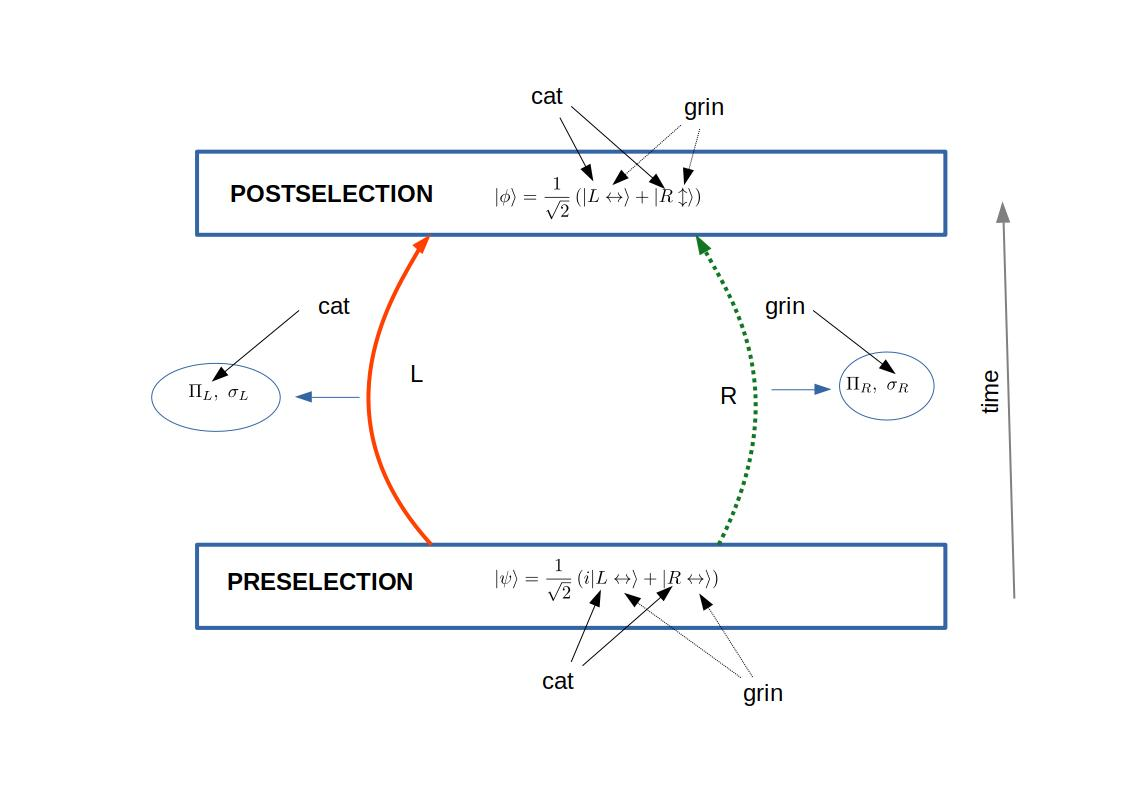
\includegraphics[width=0.8\textwidth]{ART_dajka/cat.jpg}%
 \end{center}%
 \caption{The Cheshire Cat effect. Photon in an interferometer is preselected in a~state $|\psi\rangle$.  It is then  {\it weakly} measured along left and right arms (possible $L,R$ paths)  and then postselected in a~state $\phi\rangle$. The weak values $
\langle \Pi_L\rangle^w =1$,
$\langle \Pi_R\rangle^w=0$, 
$\langle \sigma_L\rangle^w =0$ and $\langle \sigma_R\rangle^w=1$ interpreted as a~presence of the Cat in the left arm and its grin in the right one indicate separation of photon polarization (`grin') and photon position. }\label{cat}
\end{figure}
Effectively, both types of degree of freedom are qubits i.e. a~state space of the  system is
$\mathcal{H}=\mathbf{C}^2\otimes\mathbf{C}^2=\mbox{span}\{|L\rangle,|R\rangle\}\otimes\mbox{span}\{|\leftrightarrow\rangle,|\updownarrow\rangle\}$  
where $L,R$ and $\leftrightarrow,\updownarrow$ label the `external' and internal degrees of freedom respectively. 
Detection of  the Cat's position  corresponds to a~measurement related to the projectors: $\Pi_L=|L\rangle\langle L|$ and $
\Pi_R=|R\rangle\langle R|$
whereas a~measurement of Cat's grin (an internal degree of freedom) in a~given (either left or right) position requires the projectors $\sigma_L = \Pi_L \sigma_z$ and $\sigma_R =  \Pi_R \sigma_z$
where  $\sigma_z=|+\rangle\langle+|-|-\rangle\langle -|$ for $|\pm\rangle=[|\leftrightarrow\rangle \pm i|\updownarrow\rangle]/\sqrt{2}$. 
%
According to the proposal given in~\parencite{cat}, the system is preselected (prepared) in a~ specific but not entangled state
$|\psi\rangle = \frac{1}{\sqrt{2}}\left(i|L\leftrightarrow\rangle +|R \leftrightarrow\rangle\right)$
and, after passing the interferometer,  postselected in a~state
$|\phi\rangle = \frac{1}{\sqrt{2}}\left( |L\leftrightarrow\rangle +|R \updownarrow\rangle\right)$.   
%
In the meantime, one measures {\it weak values} Eq.(\ref{weak}) of the quantities $\Pi_{L,R}$ and $\sigma_{L,R}$ i.e. weak values of the Cat's position and grin respectively. One obtains~\parencite{cat}
$
\langle \Pi_L\rangle^w =1$,
$\langle \Pi_R\rangle^w=0$, 
$\langle \sigma_L\rangle^w =0$ and $\langle \sigma_R\rangle^w=1$. 
% 
Whenever a~weak value is null the corresponding quantum property (either the Cat's presence or its grin in one of two arm of the interferometer) is absent in a~particular arm  where the weak measurement was performed. With such an interpretation we infer that a~presence of the Cat (indicated by $
\langle \Pi_L\rangle^w \neq 0$) in the left $L$ arm of the interferometer is accompanied by a~presence of Cat's grin in the right $R$ interferometer's arm as indicates $\langle \sigma_R\rangle^w\neq 0$. Clearly, the description provided here is far from being complete. In particular it does not take into account specific experimental circumstances typical for realistic Cheshire Cat measurements~\parencite{dup}, recent experiments~\parencite{c2,cat_schlos} or an effect of decoherence~\parencite{schloss} modyfying weak values~\parencite{Shik} and the Cheshire Cat predictions~\parencite{mojkot,mojkot1}. Moreover, interpreting null weak value as a~hallmark of a~`{\it non-presence} of something' is controversial and  far from being commonly accepted  
~\parencite{PhysRevA.95.032110,PhysRevA.97.046103,PhysRevA.97.046102,vaid_trans,lady}. 
\begin{figure}
\begin{center}
 \includegraphics[width=0.8\textwidth]{ART_dajka/vaid1a.eps}\\%
 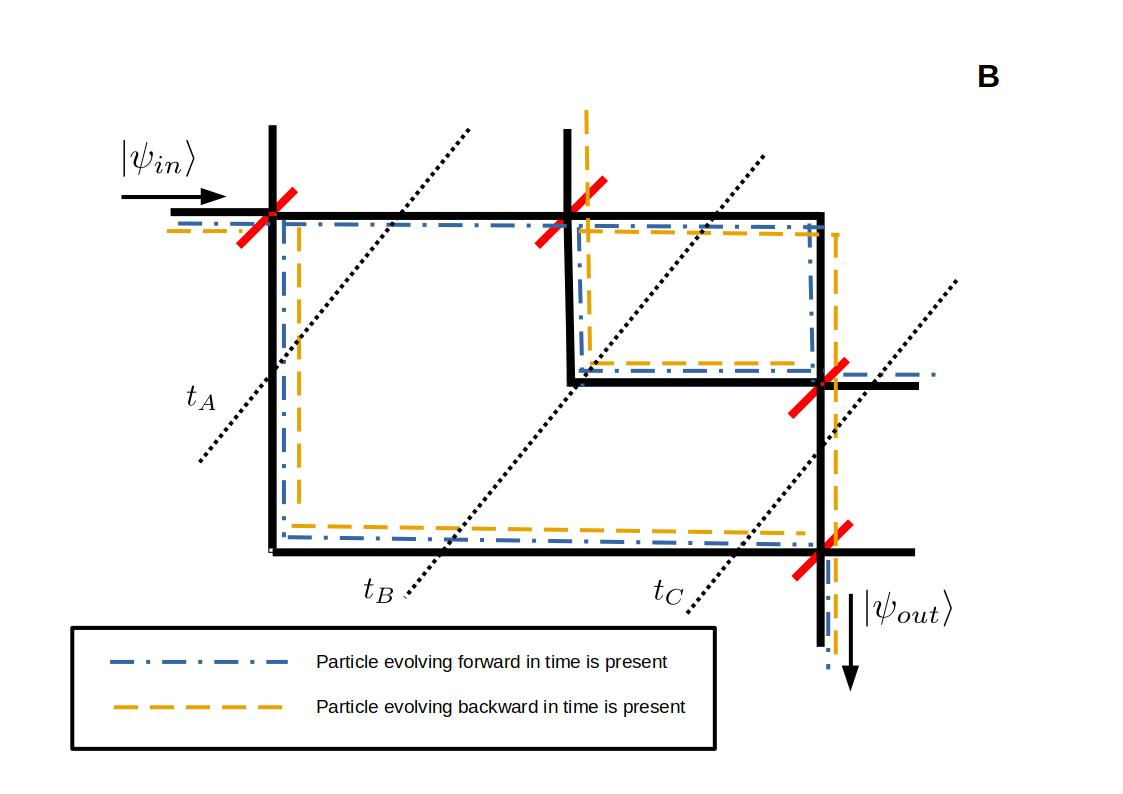
\includegraphics[width=0.8\textwidth]{ART_dajka/vaid1b.jpg}%
\end{center}
 \caption{Vaidman  interferometer consisting of four beam splitters $BS_{1,2,3,4}$ acting as unitary transformation in Eq.(\ref{bs}). In  {\it panel A} there are  three `paths' Eq.(\ref{baz}) indicted  $I,II,III$ and labelled by different colours. An entrance of an input a~particle in a~state $|\psi_{in}\rangle$ and an exit of a~particle in a~state $|\psi_{out}\rangle$ are indicated by arrows. Time instants  $t_{A,B,C}$ when  weak measurements take place are indicated by dotted lines in  {\it panel B}. The dash-dot and dash lines shown in a~legend box of {\it panel B} indicate  a~{\it non-zero} amplitude for meeting a~particle evolving forward and (respectively) backward in time. According to the TSVF the particle leaves a~faint trace only if {\it both lines} coincide i.e. on a~green path ($III$) and inside the internal interferometer as it is indicated in {\it panel B}.}\label{fig0}
\end{figure}

\section{Faint trace of a~particle in a~Vaidman interferometer}



Quantum particle can be prepared (preselected) in a~given and desired state and may also be postselected in another state with a~known at least in principle probability. That what occurs in between, what is the particle's past, remains problematic due to specific features of quantum measurements, cf. Eq.(\ref{ideal}), unavoidably modifying quantum states of measured objects. It is particularly important if one asks about a~history of a~quantum particle passing through interferometer: the particle enters the device and leaves it (if its outcome is measured), however, inside the interferometer, unless it's coherence is lost, the particle leaves nothing but a~faint trace {\it defining} its presence, a~faint trace which
is a~result of a~{\it small} change of an amplitude of a~component orthogonal to an undisturbed particle's state (weakly). Such a~faint trace is measurable  only in experiments operating on an
ensemble of particles having the same pre-- and postselection.
%
%
Past of a~quantum particle in a~nested Mach--Zehnder interferometer ({\it Vaidman interferometer})---proposed~\parencite{PhysRevA.87.052104} and presented in Figure~(\ref{fig0})---was recently studied in \parencite{PhysRevA.87.052104} using 
quantum weak values~\parencite{primus,weak,Aharonov2008} and the two state vector formalism (TSVF)~\parencite{Aharonov2008}. In this approach the faint trace is left by a~particle unless a~{\it weak value} of an appropriate projecting operator vanishes. A~weak measurement of particle traces, contrary to a~traditional and collapse assisted one, hardly perturbs the system maintaining its coherence sufficiently for interference effects to occur. The results, however, are highly confounding:  particles seem to follow anomalous {\it discontinuous} path. Such a~seemingly weird conclusion results in plethora of controversies~\parencite{PhysRevA.88.046102,PhysRevA.88.046103}, some of them are quite recent \parencite[cf.][]{lady}, and since that time  (almost) all  works  on that problem  have came in triads: a~paper, commentary inspired by the paper and a~reply to the comment~\parencite{PhysRevA.88.046102,PhysRevA.88.046103}.  
The main reason is that the TSVF~\parencite{Aharonov2008} applied in \parencite{PhysRevA.87.052104} is one of few possible approaches to investigate quantum past. The other non--equivalent alternatives are consistent (decoherent) histories~\parencite{PhysRevA.94.032115,PhysRevA.95.066101} (briefly presented below), standard quantum mechanics~\parencite{PhysRevA.96.022126,PhysRevA.99.026103,PhysRevA.99.026104} and many other other alternative studies
~\parencite{PhysRevA.91.012103,PhysRevA.93.036103,PhysRevA.93.017801,Vaidman_2018,PhysRevA.92.023829, Hashmi_2016,Hashmi_2018,elitzur}. Moreover, even recent experiments and their detailed analyses fail to resolve all the controversial issues~\parencite{PhysRevLett.111.240402,10.3389/fphy.2015.00047,10.3389/fphy.2015.00048,Sponar_2019,PhysRevA.95.042121,PhysRevA.97.052111, PhysRevA.97.052111,PhysRevA.89.033825,elitzur,WIESNIAK20182565}.  
A~conception of
discontinuous path is clearly counter--intuitive but there are analyses~\parencite{e20110854,PhysRevA.101.052119} and claims which support the faint--trace anomalous picture as experimentally confirmed.  


For a~sake of completeness we formalize the Vaidman interferometer and review the controversial features of the faint traces of particles passing it. The original Vaidman interferometer is presented in Figure~(\ref{fig0}). It consists of spatial degree of freedom given by three paths denoted by $\RN{1},\RN{2},\RN{3}$ respectively and four beam splitters. The Vaidman interferometer can effectively be described~\parencite{PhysRevA.96.022126,PhysRevA.99.026104,PhysRevA.99.026103,scirep} as a~three level quantum system (a qutrit) with a~state space spanned by an orthonormal basis
%
\begin{equation}\label{baz1}
|\RN{1}\rangle=\left(\begin{array}{c} 1 \\ 0 \\ 0   
\end{array}\right)\!,\,\,|\RN{2}\rangle=\left(\begin{array}{c} 0 \\ 1 \\ 0   
\end{array}\right)  \mbox{and}\,\,\,\, |\RN{3}\rangle=\left(\begin{array}{c} 0 \\ 0 \\ 1   
\end{array}\right)\!.
\end{equation}
%
Let us note an intuitively acceptable rationale behind imposing orthogonality on the set Eq.(\ref{baz1}): if a~particle collapses to a~particular state in Eq.(\ref{baz1}), at the same time there is no amplitude to be in an another one.  
%
In an ideal setting of a~noise--less system (for a~noisy dephasing model \parencite[cf.][]{scirep}), a~passage of a~particle is described by a~unitary transformation composed of four unitaries $U_4U_3U_2U_1$ corresponding to subsequent beam splitters termed as $BS_{i}, i=1, \ldots, 4$ in Figure~\ref{fig0}:
\begin{equation}\label{bs}
\begin{split}
&U_1 = U_4 =\frac{1}{\sqrt{3}}\left( \begin{array}{ccc} \sqrt{3} & 0 & 0 \\ 0 & -1 & \sqrt{2} \\ 0 & \sqrt{2} & 1  
\end{array}\right)\,\,  \mbox{and}\\%\,\,\,\,
&U_2 = U_3 =\frac{1}{\sqrt{2}}\left( \begin{array}{ccc} 1 & 1 & 0 \\ -1 & 1 & 0 \\ 0 & 0 & \sqrt{2}  
\end{array}\right)\!.
\end{split}
\end{equation}
The strategy applied in \parencite{PhysRevA.87.052104} to infer the path of a~particle entering  and leaving Vaidman interferometer  in a~state $|\RN{3}\rangle$  was to investigate its {\it weak trace}  at three instants $t_A,t_B,t_C$ indicated in Figure~(\ref{fig0}). In a~framework of the TSVF~\parencite{Aharonov2008} and according to \parencite{PhysRevA.87.052104} the weak trace is indicated by  a~non--vanishing weak value~\parencite{primus,PhysRevA.95.032110} of one of the  projectors
%
\begin{equation}\label{weak0}
\begin{split}
\langle\Pi_i\rangle_w^q=\frac{\langle\psi_{post}^q|\Pi_i|\psi_{pre}^q\rangle}{\langle \psi_{post}^q|\psi_{pre}^q\rangle},% \,\,\,
&\mbox{where}\,\,\,\,\Pi_i =  |i\rangle\langle i|,\,\, i=\RN{1},\RN{2},\RN{3} \\% \,\,\,
&\mbox{and} \,\,\, q=A,B,C 
\end{split} 
\end{equation}
where forward in time evolving preselected state (directly prior to the measurement of $\Pi_i$) and backward in time postselected state (immediately after the measurement) states compose  a~{\it two--state vector} $\langle\psi_{post}||\psi_{pre}\rangle$. 

Most of controversies originate from highly counter--intuitive conclusions provided in \parencite{PhysRevA.87.052104} indicating possibility of discontinuous trajectories followed by a~particle passing trough Vaidman interferometer. There are three instants $t_A,t_B,t_C$ where the weak trace is measured: $A$: just after it passes the interferometer  $BS_1$ but before it arrives to $BS_2$, $B$: where the weak measurement becomes conducted for all three potential paths and $C$: after the $BS_3$ beam splitter as presented in Figure~(\ref{fig0}). The corresponding  forward-in-time evolving preselected states read as:   
$
|\psi_{pre}^A\rangle = U_1|\RN{3}\rangle$, $
|\psi_{pre}^B\rangle = U_2U_1|\RN{3}\rangle$ and $|\psi_{pre}^C\rangle = U_3U_2U_1|\RN{3}\rangle$. 
In the time--symmetric TSVF setting the  postselected states 
$|\psi_{post}^A\rangle = U^\dagger_2U^\dagger_3U^\dagger_4|\RN{3}\rangle$, $|\psi_{post}^B\rangle =U^\dagger_3U^\dagger_4|\RN{3}\rangle$ and $|\psi_{post}^C\rangle =U^\dagger_4|\RN{3}\rangle$ describe a~hypothetical particle detected at $\RN{3}$ evolving backward in time. Results of the weak measurement are summarized in Table~(\ref{tab0}). 
%
\begin{table}[ht]
\centering
\begin{tabular}{|l||lll|ll|}
\hline
$\langle\Pi_{\RN{1},\RN{2},\RN{3}}\rangle_w^{A,B,C}$ & $\RN{1}$ & $\RN{2}$ & $\RN{3}$ &$U_{pre}^{A,B,C}$ & $U_{post}^{A,B,C}$ \\
\hline
\hline
A~& 0 & 0 & 1 & $U_1$ & $U^\dagger_2U^\dagger_3U^\dagger_4$\\
%\hline
B~& -1 & 1 & 1 & $U_2U_1$ & $U^\dagger_3U^\dagger_4$ \\
%\hline
C~&  0 & 0 & 1 & $U_3U_2U_1$ & $U^\dagger_4$\\
\hline

\end{tabular}
\caption{\label{tab0} Weak traces $\langle\Pi_{\RN{1},\RN{2},\RN{3}}\rangle_w^{A,B,C}$ Eq.(\ref{weak0}) of a~particle in Vaidman interferometer in Figure~(\ref{fig0}) at different instants $A,B,C$ indicated in Figure~(\ref{fig0}) and corresponding pre-- and postselections given by $|\psi_{pre}^{A,B,C}\rangle=U_{pre}^{A,B,C}|\RN{3}\rangle$ and $|\psi_{post}^{A,B,C}\rangle=U_{post}^{A,B,C}|\RN{3}\rangle$ respectively. It follows that at $t_A$ and $t_C$ a~particle leaves its weak trace on paths $\RN{1}$ and $\RN{3}$ respectively whereas at $t_B$ a~faint trace is present on each of three paths.}
\end{table}
According to \parencite{PhysRevA.87.052104} a~presence of a~particle is defined by 
its non--vanishing weak trace. The counter--intuitive conclusion which can be inferred upon the results summarized in Table~(\ref{tab0}) is the following: at $A$ and $C$ the particle is present in $\RN{3}$, what upon Figure~(\ref{fig0}) is intuitively acceptable, but at $B$ it is also present in an internal loop ($\RN{1},\RN{2}$) of the Vaidman interferometer.  The above formal analysis one can support  utilizing the TSVF and a~{\it sine qua non} condition for a~presence of particle: to get a~non-vanishing  
{\it weak value} of a~ particular projector in a~ weak measurement scheme  both the amplitudes of  forward and backward evolving component of the two--vector  necessarily   must  not vanish.  The regions where the amplitudes of forward and backward evolving states do not vanish are depicted in Figure~(\ref{fig0}) with dash-dot and dash lines respectively. The only regions where the lines coincide are the path labeled by $\RN{3}$ and the internal loop of the Vaidman interferometer. There is a~faint trace left by  particles  on the path $\RN{2}$ neither between beam splitters $BS_1$ and $BS_2$ (potentially used  photons entering the internal loop) nor between $BS_3$ and $BS_4$ where the photons could exit the internal loop. In simple words, upon the TSVF we conclude that a~presence of a~particle indicated by a~faint trace  in an internal loop is not accompanied by any trace of a~particle entering or leaving the internal loop and the particle path is 
{\it discontinuous}.  It is obvious that such a~confounding result needs further experimental verification. One can safely assume that any potential experiment, as it was so far, will be highly subtle and sophisticated~\parencite{e20110854,PhysRevA.101.052119,pnas,pnas1}. 







%\section{Cheshire cats and conterfactual communication}

\section{Consistent histories as an alternative}  

Orthodox (Copenhagen orthodox) researchers claim that one 
cannot talk about a~quantum particle between measurements at all. This is an obvious limitation of standard quantum theory radically excluding important questions related to a~past behaviour of quantum systems.   
%
Previously discussed  two--state vector formalism~\parencite{Aharonov2008} and consistent (or decoherent) histories approach~\parencite{Griffiths,Griffiths1984,Omnes1988,Omnes1,gel1,gel} serve  as fruitful examples of theoretical extensions  going beyond (and sometimes across) the Copenhagen interpretation. In particular,  we have recently been  witnessing how  the two above-mentioned approaches are competitively applied to a~ problem  of a~past behaviour of a~quantum particle in a~Vaidman interferometer~\parencite{PhysRevA.87.052104,PhysRevA.95.066101,scirep}. Using different methods, consistent histories allow one to gain an additional insight if they are applied to  problems  ranging from a~small but fundamental~\parencite{GRIFFITHS_measur,GRIFFITHS_onto,Griffiths2014,mea1} to the largest scale~\parencite{zur1,q_cosm}. The consistency of  histories  allows one
to assign probabilities to sequences of suitably defined events for a~quantum system. As the quantum events in this perspective  do  not rely on the notion of measurement {\it per se}, the consistent histories approach enables one to design a~new type of logical approach~\parencite{Griffiths1984} which is essentially different to the Birkhoff and von Neumann quantum logic~\parencite{qlog}. There is a~particular practical advantage of using consistent histories formalism to gain information about a~system if
an external measurement is not available either because of fundamental or simply technical reasons as it is in the case of  Vaidman interferometer where an experiment output is highly sensitive to a~measurement-induced coherence deficiency. 
%
Quantum reasoning based on consistent histories~\parencite{Griffiths_reason} uses projective decomposition of identity $PDI=\{P^k\}$ 
where $P^jP^k =\delta_{jk}P^k$ and $\sum_j P^j=I$
as its cornerstone~\parencite{Griffiths}. It   serves as a~quantum-mechanical counterpart of an event algebra used in standard stochastics. There is, however, one  crucial yet fundamental requirement which is additionally imposed: {\it the single framework rule}~\parencite{Griffiths,Griffiths_reason,GRIFFITHS_measur}. According to that rule  simultaneous reasoning to physical properties is meaningful if it is limited to  `events'  which are compatible~\parencite{Griffiths,Griffiths_reason,GRIFFITHS_measur,GRIFFITHS_onto}. 
At each time instant all  quantum properties of a~system correspond to elements of an instantaneous PDI having assigned probabilities and a~ time  evolution  of the quantum systems studied with consistent histories model can be considered as a~stochastic process. With such an approach neither 
the future nor the past states of the system must be 
determined by the present state since,  instead, they are (only) related by their probabilities. If the probabilities are 0 or 1 one arrives at a~deterministic time evolution. A~mathematical stage accommodating  sequences of events is a~tensor product of `instantaneous' Hilbert spaces. 
%
Quantum properties (events) related to time evolving systems are its {\it histories} forming time--dependent PDIs 
where (generically) $PDI(t_i)\neq PDI(t_j)$ for different time instants giving one a~chance to pose different questions concerning different quantum properties of the systems at different time instants. 
Assigning probabilities to non-commuting quantum properties  is only meaningful if there is
no interference between pairs of histories which suppose to be {\it decoherent}. 
After extending the celebrated Born rule to multi--time history  one can assign a~weight to a~sequence of events~\parencite{Griffiths1984,Griffiths,Griffiths_reason,GRIFFITHS_onto, GRIFFITHS_measur} and impose  {\it consistency condition}~\parencite{Griffiths1984,Griffiths,Griffiths_reason,GRIFFITHS_onto, GRIFFITHS_measur} satisfied by histories which are meaningful.
Let us note that a~quantum history of a~physical system is a~sequence of quantum events at successive times, where a~quantum event at a~particular time can be any quantum property of the system in question \parencite{Griffiths}. Such a~ convenient tool can  serve to analyse properties of systems that are very difficult to measure and, in particular, consistent reasoning has already been applied to study history of a~particle in a~ Vaidman interferometer. The result was that the TSVF predictions described above are based upon inconsistent histories and hence are meaningless.  Clearly, an associate debate~\parencite{PhysRevA.94.032115,PhysRevA.95.066101} was surprising to nobody.
%
Consistent histories seem to be an attractive and mathematically sound extension of quantum mechanics (or quantum stochastics) also suitable to study the past of quantum systems  or even  to dissolve the  (in)famous measurement problem~\parencite{GRIFFITHS_measur,Griffiths_reason}. The single framework rule, however, crucial for consistent reasoning, is highly more 'invasive' for quantum theory in comparison to a~simple inclusion of a~backward in time evolving postselected state as it is done in the TSVF. To avoid long and technical argumentation  to support this statement and to indicate both existing and potential problems with the consistent histories let us invoke Mermin's opinion from   
\parencite*{mermin}:
\myquote{[But] I~am disconcerted by the reluctance of some consistent historians to
acknowledge the utterly radical nature of what they are proposing. The relativity of time was a~pretty big pill to swallow, but the relativity of reality itself is
to the relativity of time as an elephant is to a~gnat.}

\section{Concluding (yet not conclusive) remarks}

Weak values, contrary to standard eigenvalues, are still waiting for a~commonly accepted interpretation. In an absence of the eigenstate-eigenvalue link it is not obvious if weak measurements and their outputs can credibly describe `elements of reality' and properties of quantum systems ~\parencite{Matzkin_prop,vaid_trans}. It is agreed that weak values possess certain non--trivial predictive value and they are related, at least to some extent, to real properties of physical systems. Unfortunately, it is difficult to assign any `hard' limits of their applicability. Life would be definitely simpler if weak values were strongly measurable. In particular,  
  physical meaning of vanishing weak values applied in  a~current context of a~past of quantum systems  remains disputable~\parencite{PhysRevA.95.032110,PhysRevA.97.046102,PhysRevA.97.046103,weak,lady} although  there are analyses and experiments~\parencite{e20110854,PhysRevA.101.052119,pnas,pnas1} which support the faint--trace anomalous picture as experimentally confirmed.   

Time-symmetric description of quantum systems utilizing the TSVF~\parencite{aharonov_entrop,Aharonov2008}, despite certain problematic issues concerning its adaptation to open quantum systems requiring mixed states for their description~\parencite{weak,scirep},   seems to be less controversial. At the same time, however, it affects new research areas such as counterfactual reasoning~\parencite{kont0}  or even the hot-forever {\it free will problem}~\parencite{wil}. 

Counterfactuality and counterfactual reasoning (`if it were $a$, then it would be $b$')~\parencite{kont_book,kont0}  is a~natural  extension of an interaction-free measurement, cf. Elitzur
and Vaidman’s interaction-free bomb detector~\parencite{bomb}, where a~bomb (a~detector, using more pacifistic terminology) indicating a~presence of a~single photon is put in
one of the arms of a~Mach–Zehnder interferometer. Even if the
bomb does not blow up, its  presence  affects an interference pattern  at the output of the interferometer.  Direct application of the Aharonov-Bergman-Lebowitz rule Eq.(\ref{abl}) for counterfactual reasoning is not always sufficient and acceptable~\parencite{kont0}. The idea of using a~time-symmetric approach to quantum counterfactuals has  recently  found a~promising application in quantum-based counterfactual communication. Such communication protocols are counterfactual by using quantum effects to send
messages without any matter or energy transfer between communicating
parties~\parencite{kont1,kont2}). There are already known crypto protocols~\parencite{kont_crypto, kont_crypto0,kont_crypto1,kont_crypto1,kont_crypto2} based upon that idea.
Obviously, all the controversies concerning weak values, past of quantum systems and counterfactual reasoning both mentioned and not mentioned in this work to be resolved need to be supported by further experimental investigations. 

One can conclude that with a~tremendous development of highly sophisticated  experimental techniques we are faced (maybe for the first time) with problems which {\it simultaneously} require advanced technology, fresh and flexible theory and, last but not least, sound interpretation. Let us take up this challenge.    
 

\end{artengenv}

\begin{artengenv}{Walter Block}
	{Response to Wysocki on indifference\footnotemark{}}
	{Response to Wysocki on indifference}
	{Response to Wysocki on indifference}
	{Loyola University New Orleans}
	{Nozick
%	(1977)
	\parencite*{nozick_austrian_1977}
	was a~critique of the view of Austrian economics which rejected the notion of indifference in human action. This author claimed that this stance was incompatible with the notion of the supply of a~good, and, also, with diminishing marginal utility, both of which were strongly supported by this praxeological school of thought. Block
%	(1980)
	\parencite*{block_pu1}
	was an attempt to rescue the Austrian school from this brilliant intellectual challenge. Hoppe
%	(2005, 2009A)
	\parencites*{hoppe_pu1}{hoppe_further_2009}
	rejected Nozick's challenge, and, also, Block's
%	(1980)
	\parencite*{block_pu1}
	response. Block
%	(2009A)
	\parencite*{block_rejoinder_2009}
	and Block and Barnett
%	(2010),
	\parencite*{block_rejoinder_2010},
	defended Block's
%	(1980)
	\parencite*{block_pu1}
	analysis of indifference. The latest contribution to this ongoing discussion is Wysocki
%	(2021)
	\parencite*{wysocki_problem_2021}
	who maintains that Hoppe was correct in his rejection of Nozick, while Block was not. The present paper is a~rejoinder to Wysocki
%	(2021).
	\parencite*{wysocki_problem_2021}.
	}
	{indifference, supply, diminishing marginal utility, praxeology.}


\footnotetext{I~wish to thank two referees of This Journal for helpful comments on an earlier version of this paper which when incorporated greatly improved it. The usual caveats of course always apply.}

\section{Introduction}
\lettrine[loversize=0.13,lines=2,lraise=-0.01,nindent=0em,findent=0.2pt]%
{W}{}ysocki
%\label{ref:RND6Uy0JUU7mC}(2021)
\parencite*[][]{wysocki_problem_2021} %
 is written in support of Hoppe 
%\label{ref:RNDWGhcRWeJic}(2005; 2009)
\parencites*[][]{hoppe_pu1}[][]{hoppe_further_2009} %
 in his debate with Block 
%\label{ref:RNDmWQ6OyRVB5}(2009a)
\parencite*[][]{block_rejoinder_2009} %
 and Block and Barnett 
%\label{ref:RNDqkpBujF28F}(2010).
\parencite*[][]{block_rejoinder_2010}. %
 This dispute concerns the best way to counter Nozick's 
%\label{ref:RNDXoqIUUtNTR}(1977)
\parencite*[][]{nozick_austrian_1977} %
 rejection of Austrian praxeological economics which involves indifference, the supply of a~good, and the law of diminishing marginal utility.

I~will be quoting widely from Wysocki
%\label{ref:RNDOJxzE3ycVb}(2021)
\parencite*[][]{wysocki_problem_2021}%
\footnote{All references to Wysocki, unless otherwise indicated, will be to this one article of his.} and then responding to his many, and important points. Let us begin.

According to Wysocki
%\label{ref:RNDHYmAGPUCkC}(2021):
\parencite*[][]{wysocki_problem_2021}:%


\myquote{
If he were forced to give up a~unit of apple juice or the (sic) one of mineral water, he would be indifferent between the two.
}

Before responding to this quote, let me try to give the reader the context. I'm going to be putting ``words into the mouth'' of this author, but, hopefully, I~will be accurately transmitting his overall viewpoint. In my understanding of what he is about, he is supporting Hoppe's criticism of my critique of Nozick. All three of us, Hoppe, Wysocki and me reject Nozick's criticism of Austrian economics; but Hoppe and Wysocki maintain that my rejection of Nozick is a~failure. The issue turns on indifference and the supply curve. All economists, Austrian or not, maintain that there is such a~thing as a~supply curve. If this is to exist, avers Nozick, then the economic actor such see every element of the supply as equivalent. If there is to be a~supply curve of apples, for example, the consumer must see all the apples as the same; he must be indifferent between them. If he is not, if he sees some apples as different from others, there cannot be one supply curve of apples; there must be two or more, depending upon how many types of apples are perceived. However, asserts Nozick, correctly, Austrians reject the concept of indifference; they are thus logically inconsistent in acquiescing as to the supply curve.

Let me now respond to this opening quote from Wysocki, who rejects Nozick's critique of Austrianism, and supports Hoppe's criticism of my critique of Nozick. My claim is that Austrians can have our cake and eat it too; we may acknowledge the legitimacy of the supply curve (the demand curve too), and still not buy into the concept of indifference, at least not when choices are being made.

I~just do not see how anything like this could be true. For if this economic actor gave up one of these economic goods, that would, surely, demonstrate
%\label{ref:RNDn4BKSh14VO}(Rothbard, 2011 [1956])
\parencite[][]{rothbard_toward_2011} %
 that he valued it less than the other; and vice versa. The point is, there is no way he could reveal, in action, that he was indifferent between these two items.

If he were truly ``indifferent between the two'' then of course, a~la Wysocki, he could not choose to set aside either. However, this contradicts this author's premise. He states that the economic actor was \textit{forced} to give up one unit of either the juice or the H\textsubscript{2}O. We much assume he complied. If so, he might well have tossed a~coin to determine which one he gave up, but, in going along with the coin toss, he is not acting in an indifferent manner. Logically, he cannot do any such thing.

Our author continues:

\myquote{
Specifically, indifference has such a~propositional content (believing that \textit{x} and \textit{y} are economically identical) that it cannot motivate an actor to act on it.
}
But this appears to be a~direct contradiction of his previous statement. If indifference ``cannot motivate'' someone to undertake an action of picking and choosing and setting aside, how can the person in question objectively reveal that he saw the apple juice and mineral water as equivalents?

Wysocki then avers as follows:

\myquote{
Specifically, indifference has such a~propositional content (believing that \textit{x} and \textit{y} are economically identical) that it cannot motivate an actor to act on it. By contrast, homogeneity is a~relation holding between economic goods. However, remember that economic goods are not mere physical goods.
}

Whenever a~person engages in human action, giving up a~gallon of water or purchasing an extra bottle containing this amount of H\textsubscript{2}O, he cannot be engaging in an act of indifference between his present stock and the additional unit. Indeed, there is no such thing as an ``act of indifference.'' There can only be acts of preference and of setting aside. People can only be preferring or setting aside; e.g., treating these units as \textit{different} from one another. A~supply curve, then, consists of goods that are seen as physically indistinguishable one from the other in the absence of any human action that takes place with regard to them.\footnote{That would be a~necessary condition. But not sufficient, for we must incorporate Machaj's
%\label{ref:RNDp032hAJ439}(2007)
\parencite*[][]{machaj_praxeological_2007} %
 insightful example of the same physical ring on the hand of one's fiancé, and another physically identical one in the jewelry shop   
%\label{ref:RND9f7aYwJ7kb}(Block, 2009b; also, 2012).
\parencites[see][]{block_rejoinder_2009-1}[also][]{block_response_2012}.%
}

In the view of Wysocki:

\myquote{
When asked how we should understand the concept of the same good presupposed by the universal law of time preference, an Austrian economist might reply in a~similar fashion: we can easily learn whether \textit{x}\textsubscript{1} (some economic good at \textit{t}\textsubscript{1}) and \textit{x}\textsubscript{2} (some economic good at \textit{t}\textsubscript{2}) are the units of the same good. We would do so by checking whether an actor would now necessarily prefer \textit{x}\textsubscript{1} to \textit{x}\textsubscript{2}.
}
But how are we to ``check'' whether that is true or not? All we can observe is human action: people choosing amongst alternatives. It is logic alone, not any presumably empirical ``checking'' that can make any such determination. But Wysocki rejects this as ``tautologies.'' He states in this regard:

\myquote{
But these two apodictically true statements come at a~price. For the consequence of the lack of the independent (of the laws in question) notion of the same good, would turn those laws into concealed tautologies.
}

This author continues:

\myquote{
Incidentally, similar remarks would apply to Austrian formulation of the universal law of time preference. Austrians hold that for one (and the same!) end, each actor would prefer to achieve it sooner rather than later. Note, this law also presupposes the notion of the same good—but this time in a~sort of a~temporal way for it is the same economic good that is carried over time (we may obtain it at \textit{t}\textsubscript{1}or at \textit{t}\textsubscript{2}). When asked how we should understand the concept of the same good presupposed by the universal law of time preference, an Austrian economist might reply in a~similar fashion: we can easily learn whether \textit{x}\textsubscript{1}(some economic good at \textit{t}\textsubscript{1}) and \textit{x}\textsubscript{2} (some economic good at \textit{t}\textsubscript{2}) are the units of the same good. We would do so by checking whether an actor would now necessarily prefer \textit{x}\textsubscript{1} to \textit{x}\textsubscript{2}. But these two apodictically true statements come at a~price. For the consequence of the lack of the independent (of the laws in question) notion of the same good, would turn those laws into concealed tautologies.

}
Our author continues in his footnote 13:

\myquote{
In fact, it was Rothbard
%\label{ref:RNDbm0hE646An}(2011, pp.15–16)
\parencite*[][pp.15–16]{rothbard_toward_2011} %
 himself who resorted to this tautologous defense of the universal law of time preference, which is evidenced by the following passage: ‘Time preference may be called the preference for present satisfaction over future satisfaction or present good over future good, provided it is remembered that it is the same satisfaction (or ``good'') that is being compared over the periods of time. Thus, a~common type of objection to the assertion of universal time preference is that, in the wintertime, a~man will prefer the delivery of ice the next summer (future) to delivery of ice in the present. This, however, confuses the concept ``good'' with the material properties of a~thing, whereas it actually refers to subjective satisfactions. Since ice-in-the-summer provides different (and greater) satisfaction than ice-in-the-winter, they are not the same, but different goods. In this case, it is different satisfactions that are being compared, despite the fact that physical property of the thing may be the same. Whereas in the body of the text we considered the possible Austrian rejoinder in the form of saying that the same good can be conceptualized as the one that obeys the universal law of time preference, Rothbard merely contraposes by saying that if there is an apparent preference for a~future good (ice cream in summer) over a~present good (ice-cream in winter now), these two cannot constitute one and the same economic good. So, not only is the Rothbardian solution clearly circular, but also it gives the impression of fudging the notion of the same good. It may seem that whatever counterexamples to the law of time preference one may possibly come up with, Rothbard would rebut it by claiming that his critic invokes two distinct economic goods. This is yet another indication that an independent concept of the same good is logically required.
}

There are problems with this analysis. A~tautology gives us no information about the real world. Rather, it merely indicates definitions. For example, ``bachelor'' is an ``unmarried man.'' This insight offered by Rothbard and rejected by Wysocki constitutes much more: it is a~synthetic apriori statement which is both necessarily true and, also, give us profound insight as to how the real world operates. As to ``fudging'' this seems an erroneous characterization. Let us consider a~different case. It is alleged that ``two things cannot be in the same place at the same time.'' Someone objects: but more than two people can both be in New York City at the same time. The ``fudger'' responds: that's too big a~``place.'' Whereupon the critic says: but more than two people can both be in Manhattan at the same time, and that borough is smaller than the entire city.'' What is the ``fudger'' to do but to ``fudge'' once again? And to keep on doing so until the critic gives up. But ``fudging'' is not the correct description of this process. ``Clarification'' would do much better.

Wysocki states:

\myquote{
First and foremost, Nozick's challenge may be construed as a~purely logical objection to Austrian repudiation of indifference. After all, remember, the gist of Nozick's objection was that without the concept of indifference, Austrians would be unable to formulate the law of diminishing marginal utility. Indubitably, in this respect Nozick is right. The law of diminishing marginal utility has it that when we deal with a~supply of economically same units, each additional unit we value less; or, in other words, each additional unit is of lower utility.
}

To my way of thinking, this all depends upon precisely what is meant by ``when we deal with.'' If ``dealing with'' means, merely, contemplating a~stock of goods, then ``indifference'' is quite acceptable. After all, it is a~perfectly good word in the English language. Mere contemplation is not a~human action, at least not vis a~vis the object of the contemplation.\footnote{It is a~human action insofar as it indicates that the person prefers to contemplate at this moment in time when he could have been doing something else, which he sees as a~lesser value to him.} But if ``dealing with'' is taken as acting with regard to, say, a~stock of goods, then, it depends upon the precise action. For example, suppose someone sells the entire stock to someone else. Then, again, indifference vis a~vis elements of the stock with each other, is again acceptable.\footnote{Here, there would be no question of indifference between the entire stock and the money the vendor receives in payment for it. Clearly he prefers the latter.} But, if he sells only one of these units, for example the 72\textsuperscript{nd} one of them out of a~holding of 100, then he demonstrates that he prefers the other elements to this one.

Here is our author once again:

\myquote{
Second, we must also concede to Nozick that pricing of the commodity also seems to rest on the notion of indifference. Then, if Austrians fail to somehow accommodate indifference into their theory, this would have disastrous consequences for their entire conceptual edifice. After all, it must be borne in mind that the market (equilibrium)price of a~given product is a~function of supply and demand. And the demand curve is but a~reflection of the diminishing marginal utility of a~given product. That is, the demand curve—rather unsurprisingly—slopes downwards because the more we have (of a~given product), the less we value marginal units. And it is precisely why we are ready to buy more(of pretty much anything)only when the successive units of the product in question cost less and less. Therefore, it is clear to see that the demand curve reflects the logic of diminishing marginal utility. Hence, Nozick is right.
}

I~do not agree with Nozick's attack on Austrian economics. A~supply curve consists of a~locus of points indicating prices and quantities. We refer here to quantities of goods, of course, such as apples, or shoes. Are we indifferent amongst all of these objects? Of course we are. We have not yet acted upon any of them. When and if we do, we can no longer be indifferent between them. If we choose one of them, we will have demonstrated preference, not indifference. Says Nozick (paraphrase on my part): ``Aha! You Austrians are logically inconsistent. You admit that indifference is required if the supply of a~good is to make any sense.'' But there is no inconsistency. Of course, indifference is all around us.\footnote{In the television series Mary Tyler Moore, ``love was all around us.''} It only breaks up when we actually \textit{do} anything with regard to this supply, such as buy or sell any of it. In like manner, the same holds true for diminishing marginal (ordinal!) utility. We have the proverbial three bottles of water. We are indifferent between them all. They are now just sitting there. They all have precisely the same chemical properties (H\textsubscript{2}O) and we have no psychic preferences amongst any of them. We cannot so much as tell the difference between them. But then, for some reason we have to give up one of them. A~robber demands this of us, and we decide to comply. We are still indifferent between them. So, we grab one, at random. Behold, we are no longer indifferent! By our own action, we reveal that we prefer the other two bottles to this one; that is why we are giving up this one, and none other, to the thief. Has Nozick upset any Austrian theory? I~cannot see how he has. Is this mode of refuting him fallacious as Hoppe contends, and, now Wysocki? I~cannot see my way clear to agreeing with that, either. I~fear that Wysocki is giving away too much of the Austrian store to Nozick in his concession: ``Hence, Nozick is right.''

Rather, we can have our cake and eat it too. When indifference is required, in the absence of human action, in order to undergird diminishing marginal utility, or the supply and demand curves, we can retain it. But when human action takes place, we can jettison this concept.

We need not concede anything whatsoever to Nozick
%\label{ref:RND7GdaAbhB3f}(1977)
\parencite*[][]{nozick_austrian_1977} %
 in this regard. He asserts that indifference is required to demonstrate diminishing marginal utility. It is not. Before action, yes, there is indifference. There are stocks, supplies of goods, after all. But, when action occurs, when a~unit of the good is given up, or added, there is preference, not indifference.

We now arrive, more specifically, at Wysocki's dissatisfaction with my
%\label{ref:RND1yWgqppOJP}(Block, 1980)
\parencite[][]{block_pu1} %
 attempted refutation of Nozick 
%\label{ref:RND17GJmsskmJ}(1977).
\parencite*[][]{nozick_austrian_1977}. %
 Wysocki is kind enough to credit me (and my friend and colleague Hoppe) with ``eloquence'' and for having ``contributed most to the entire debate in question'' and I~am grateful to him for that compliment.

But then he offers his critique:

\myquote{
Block's account\footnote{In Block
%\label{ref:RNDYCAKJC3fjs}(1980)
\parencite*[][]{block_pu1} %
 I~mentioned 100 pounds of butter, among and between which the owner was initially indifferent, but then for some reason had to give up one of these units. He chose the 72nd one.} is doomed to conclude for it is inherently unable to square the two apparent facts: 1) that those units of butter are really (ex hypothesi) ‘equally useful, desirable, serviceable' and 2) that 72\textsuperscript{nd} one was ‘picked up'. As we are about to see, the whole problem trades on the concept of ‘picking up'. Block seems to be lured into thinking that the imagined actor does pick up the 72ndunit where he says: ``For if the person didn't really prefer to give up this (72\textsuperscript{nd}) one, why did he pick it to be given''. Fair enough, if we assume that he did pick up this very unit, he must have preferred giving up this one to giving up any other, which simply logically follows from the concept of ‘picking up' employed herein. And yet, why should we beg any questions? It is to be established first that the actor does indeed pick up the 72\textsuperscript{nd} unit. For settling this issue has a~bearing on whether he prefers giving this unit to any other or he does not. And this in turn determines whether the actor conceives of the 72\textsuperscript{nd} unit as the unit of the same supply (with all the other units of butter) or he conceives of the stock before him as consisting of two distinct classes: a) a~homogeneous class of 99 units (still intact) and b) a~singleton containing the very pound of butter given up. Therefore, it seems that something has to give here: either 100 units were not in fact perceived as equally useful or they indeed were but the actor did not (in a~relevant sense) choose to give up the 72ndunit. So, Block cannot have it both ways.
}

It seems to me that I~can indeed ``have it both ways.'' Not, of course, necessarily, with the 72\textsuperscript{nd} unit, but with any pound of butter. In the example, the owner of the butter is just sitting there, perhaps, contemplating his butter stock, and congratulating himself upon his ownership of it. If he is of a~philosophical bent, and contemplates which of these butter units he likes best, he could readily admit that he sees them as a~homogeneous blob, and is indeed indifferent between them all. But then comes a~robber who tells him, at the point of a~gun, to select one of these pounds of butter and give it to him. Or perhaps, he faces a~customer, who wants to buy one of them. Now, the situation is going to hit the fan. The grocer must choose one of these one-pound packages, to give to the thief/customer. In my example, I~chose the 72\textsuperscript{nd} unit. But I~am hardly wedded to that number. It could be any unit. But, in the event, based on the example, he must choose one of them. Let us say he chooses the first one, because he closes his eyes, and just happens upon that one. Well, now, he is no longer indifferent. Even Wysocki admits the truth of this when he says: ``Fair enough, if we assume that he did pick up this very unit, he must have preferred giving up this one to giving up any other, which simply logically follows from the concept of ‘picking up' employed herein.'' I~insist I~can indeed ``have it both ways.'' There are two separate scenarios here: one, before the demand on the part of this other person for some butter, and the other after this takes place. In the first place there is indifference, plenty of it.\footnote{Don't ask me how much. There is no such thing as a~unit of indifference.} In the second place, there is no such thing. Wysocki in my view places insufficient attention to this two-stage situation. The two scenarios are very, very different.

Wysocki continues:

\myquote{
The problem with this contention is that Block must either invalidate his assumption that they were homogeneous before the choice in order to explain why the choice (i.e. picking up the least preferred unit of butter, as opposed to the remaining ones) took place. Alternatively, if he maintains that the units in question are indeed equally useful, then he cannot explain why this particular unit of butter was picked up because they were assumed to be equally valuable in the first place. Nozick's challenge comes with vengeance to Block and the reason is precisely that the latter author has a~distorted idea of choice.
}

This author then touches upon various subjects: the essence of choice, the infinite varieties thereof, probability, numerous types of bread, many routes to super markets, the fact that I~am ``left with no hope of intelligibly conceiving of the same commodity,'' why the 72\textsuperscript{nd} unit as opposed to any old ``a'' unit? My answer might be overly simplistic; let me try it on for size in any case. The choice of the 72\textsuperscript{nd} unit was random. It was totally and completely arbitrary, used for illustration purposes only. I~fear that Wysocki does not give full credence to the very different thoughts and behavior of the butter owner before and after he is called upon to give up one unit of butter. Before? Homogeneity, to be sure. After? Heterogeneity is the order of the day. Why this should be shocking, why impossible, why positing this to take place should be logically inconsistent, is beyond me. Time changes all sorts of things; why not this too?

We then arrive at Wysocki's second interpretation of my response to Nozick; it is true and correct, but merely trivial: ``On the second reading, Block's position may be rendered true but then it would amount to the mere restatement of the law of marginal utility.'' My first reaction to this is ``Please don't help me so much,'' or ``With friends like this, who needs (intellectual) enemies'' \parencite[in this regard see][]{riley_please_2016}. %
%\footnote{See
%%\label{ref:RNDlE6uwhcc55}(Riley, 2016)
%\parencite[][]{riley_please_2016} %
% in this regard.}
 On a~more serious note, I~fail to see how my distinction between before and after human action amounts, merely, to restating the law of diminishing marginal utility. It cannot be denied, of course, that with the 72\textsuperscript{nd} unit of butter out of the way, all the others are now of greater value, but this hardly is what my refutation of Nozick is all about.

It is more than passing curious that in the next section of his paper, where Wysocki claims that Hoppe's refutation of Nozick is vastly superior to my own feeble attempt, that we read this incisive and correct statement of his: ``[…] indifference cannot be demonstrated in action, as is usually reiterated by Austrians
%\label{ref:RNDkBDnhlt2jA}(Block, 2009a; Block and Barnett II, 2010; Rothbard, 2011).
\parencites[][]{block_rejoinder_2009}[][]{block_rejoinder_2010}[][]{rothbard_toward_2011}. %
 By no means can we deduce from any actual choice whether we were confronted with the units of the same good or with the ones of distinct goods.'' But this is precisely the point I~employed to launch my critique of Nozick, to which Wysocki gives the back of his hand.

In section 5 (``Hoppe's account as a~remedy for Block's shortcomings'') of his paper, Wysocki will demonstrate that while my disproof of Nozick's criticism of Austrian economics fails, Hoppe's succeeds. Given that this is his goal, he gets off on the wrong foot. He opens with this statement:

\myquote{
First and foremost, it must be noted that—unlike Block's solution—[…] (Hoppe's) […] involves both doing justice to indifference (at least admitting that a~man can be genuinely indifferent between some options) and barring it steadfastly from the realm of choice. Briefly speaking, Hoppe
%\label{ref:RND6dL2T23Yfz}(2005)
\parencite*[][]{hoppe_pu1} %
 maintains that one cannot make a~choice under indifference.
}
But I~too, do this. There is not a~dime's worth of difference between Hoppe and me on this issue. We both acknowledge that choice, or human action, is incompatible with a~state of indifference! We both, Hoppe and I, agree with, in Wysocki's words: ``the truth of the proposition that a~man cannot choose when indifferent.''

Wysocki's account gets curiouser and curiouser. He continues: ``Specifically, Hoppe defines choice in such a~way that it entails the lack of indifference. That is, if man chooses x~over y, he is not (and, logically speaking, cannot) indifferent between the two.'' Well, Hoppe is not the only one to point to this insight. That is precisely my position, too.

However, Wysocki does not continue down this path. Instead of failing to see that Hoppe and I~are on the same page, he now, correctly, notes a~deviation between the two of us, and error number two on his part, supports Hoppe's incorrect position; writes our author:

\myquote{
Likewise, a~mother who sees her equally loved sons Peter and Paul drown and who can only rescue one does not demonstrate that she loves Peter more than Paul if she rescues the former. Instead, she demonstrates that she prefers a~(one) rescued child to none. On the other hand, if the correct (preferred) description is that she rescued Peter, then she was not indifferent as regards her sons.
}
No, no, no. While it is of course true that this poor mother\footnote{The movie ``Sophie's choice'' subjects a~poor woman to this excruciating choice.} ``prefers one rescued child to none'' she also places a~higher value on Peter than Paul. She did rescue the former, when she could have chosen differently, and selected the latter for retrieval, did she not? I~simply cannot understand how it can be denied that she favored Peter over Paul, in the face of her action in rescuing Peter, not Paul.

Wysocki's account violates the spirit of praxeology. Now, it is quite alright to do so, at least in terms of congruence with mainstream economics. Our author is here on firm ground in this regard. My argument is that both Wysocki and most economists are in error here. I~simply do not see how it is possible to deny that since the mother chose Peter, not Paul, she was not indifferent between them. Even if she did this with her eyes closed, and just grabbed the nearest son, this I~think is the correct view.

Suppose she was offered the choice between a~chicken dinner and a~fish dinner. And, she selects the former. If Wysocki and Hoppe stick to their ``logic'' they would of course be correct in concluding that the woman preferred to eat dinner rather than go hungry. But they would be logically precluded from, also, maintaining that she preferred chicken to fish. The two of them, on the one hand, and I, on the other, live on different planets. Or, perhaps Mises was incorrect in his castigation of polylogism; there are two different ``logics'' at work in this case, mine and theirs.\footnote{I~am of course joking about this. Mises was correct, as am I~in this case. The same cannot be said for Hoppe and Wysocki.}

Wysocki misconstrues Buridan's ass in the same manner. This beast, let us say, chooses the bale of hay to the right. The correct interpretation of this is two fold: one, this creature preferred life to death, and, two, he favored the hay on the right to the hay on the left. In Wysocki's correct interpretation of Hoppe, and his own, only the first is true. The second, amazingly, is not. But, but, but, the donkey moved to his right, not his left! If this is not evidence that he preferred the right to the left bale, there can be no such thing as evidence, at least not in cases like this.

At least Wysocki is logically consistent. Let us give credit where it is due: he makes the same identical mistake when it comes to the butter example. He writes:

\myquote{
[…] since the actor did indeed give up the 72nd pound of butter (while holding all of them equally serviceable), he must have preferred giving up a~unit of butter for some pecuniary equivalent. In other words, the actor preferred one unit of butter less, but some increment of money to retaining his entire stock of butter but depriving himself of an opportunity to earn this money. The second possibility is that the correct description of an action is that the actor really dispreferred that 72\textsuperscript{nd} unit that he actually gave up. If so, that unit was not the same economic good as all the other units in the first place and therefore, trivially, the original supply of 100 units was heterogeneous.

}
Again, I~say, no, no, no. Why is it so hard to realize that one and the same thing can be altogether different, given the passage of time? At time \textit{t}\textsubscript{1}, before any choice was made, yes, all units of butter were ``equally serviceable.'' Their owner was indifferent between all of them. They were homogeneous as far as he was concerned.\footnote{If he thought about it at all, which he almost certainly did not.} But then, at time \textit{t}\textsubscript{2}, when push came to shove, the grocer had a~decision to make: he valued the money more than a~unit of butter, any unit of this product, to be sure. In the event, he was compelled to choose one of them if he wanted to make the sale. If this does not establish that he valued this particular one, the 72\textsuperscript{nd} unit, less than the others, then there is no such thing as choice, utility, economic theory, common sense.

Wysocki characterizes the Peter and Paul example as ``the celebrated Hoppean thought.'' Sure.

Here we come to the very core of why our author favors Hoppe's analysis vis a~vis mine. Says Wysocki:

\myquote{
Block's point against Hoppe would be decisive if the act of saving a~particular child (under this description) instead of another were inherently preference-implying. That is, Block would succeed if we can infer from the fact of saving a~particular child (or from bringing about the event of a~particular child being saved) that this particular child was preferred to the other. Yet, there is a~deep distinction favored by Davidson
%\label{ref:RNDjKlYmL9Ybk}(2001)
\parencite*[][]{davidson_agency_2001} %
 between what an actor does (including his primitive action consisting in his bodily movements up to everything they cause) and what he does intentionally. As Davidson 
%\label{ref:RNDPGPvETu7dU}(2001, p.45)
\parencite*[][p.45]{davidson_agency_2001} %
 put it: ``[…] although intentionality implies agency, the converse does not hold''. Therefore, it would simply beg the question to say that by the act of saving Peter the mother demonstrated her preference for Peter over Paul. As established above by alluding to the Davidsonian insight, from the event that the mother authored, we cannot infer which aspects thereof were informed by her preference. Therefore, not to beg any questions, we should treat the act of saving Peter in the non-choice- (and hence also non-preference) -implying sense. Alternatively, just to remain neutral on whether the mother did actually choose to save Peter or chose to save a~child, we could say that what the mother in fact did was to save Peter. After all, to say that the mother saved Peter is only to attribute her agency to this event (in other words, it is to say that she authored the event of Peter having been saved), which does not imply that she saved Peter intentionally. And this is the key insight which, in our view, counts in favor of the Hoppean account.
}

I~have no problem with what Davidson writes. My difficulty concerns the manner in which Wysocki utilizes that insight in behalf of his own views and those of Hoppe. Why? Davidson's perception is a~matter of psychology, not praxeology. But we are now in the latter realm, not the former. Remember, this is Austrian economics we three are defending against Nozick's critique. As psychologists, we are undoubtedly interested in whether something is intentional or not. But I~insist, this is not the case in our role as praxeologists. Suppose someone shoves two plates of ice cream at you and demands you choose one. You are very busy with something else. You reach out and grab one. You are not aware of which flavor you now have at your disposal. You may be so concerned with these other matters that the actual taste of this treat does not even register with you. As psychologists, there is no objection, at least not stemming from the present quarter, in saying that you were totally unaware of what you were doing, at least ice cream wise. The other matter took all of your intention. But, in sharp contrast, we as praxeologists must note that you actually reached out and grabbed one of them, not the other. This is the essence of Hoppe's error, with support from Wysocki. That mother reached out and saved Peter not Paul. What might well have been on her mind had nothing to do with Peter nor Paul. It might well have been as Hoppe opined, she was just preferring to save one of her sons, rather than none. Who knows, she might have been thinking about ice cream, as far as we praxeologists are concerned. This does not matter in the slightest for the praxeologist. We see her grabbing Peter, not Paul, to safety, and we are compelled by praxis logic, e.g., praxeology, to note that she was not indifferent between her sons, she could not have been indifferent between them, given that she chose the one, not the other. In not seeing this, in maintaining the very opposite, Hoppe and Wysocki are guilty of what Rothbard
%\label{ref:RNDFnt7pkdLRp}(2011 [1956])
\parencite*[][]{rothbard_toward_2011} %
 labeled the error of psychologizing:

\myquote{
Psychologizing is a~common error in utility analysis. It is based on the assumption that utility analysis is a~kind of ‘psychology,' and that, therefore, economics must enter into psychological analysis in laying the foundations of its theoretical structure. Praxeology, the basis of economic theory, differs from psychology, however. Psychology analyzes the how and the why of people forming values. It treats the concrete content of ends and values. Economics, on the other hand, rests simply on the assumption of the existence of ends, and then deduces its valid theory from such a~general assumption. It therefore has nothing to do with the content of ends or with the internal operations of the mind of the acting man.
}

Consider an additional illustrative example. A~man chooses women who do not respect him. He has a~long trail of such psychologically unsatisfying and debilitating relationships. He knows he should select a~different kind of women the next time he is free to do so. But when the occasion again arises, he conforms to the same old sick pattern. A~psychologist might analyze this series of events by saying that the man full well knows what he is doing is counter-productive, and that he really wants a~better relationship with a~nice woman. But the Austrian praxeologist is precluded from making any such determination. He is required to look, only, at human action, actual behavior, and conclude that the man really prefers that type of woman.

Like a~good psychologist, Wysocki places great weight on ``what the mother intended to do'' regarding her two sons. But as praxeologists, we are forbidden to even take this into account to the slightest degree. Rather, we are (logically) required to ignore that entirely, and focus, instead, on the decision she actually made. She was \textit{not} indifferent between her two sons, as matters unfolded. What went through her mind at the actual point of choosing is entirely irrelevant. We praxeologists must focus, only, on the decision she actually made.

Nor will Parfit's
%\label{ref:RNDGya77ZS3Ig}(2011, p.289)
\parencite*[][p.289]{parfit_what_2011} %
 analysis save Wysocki's nor Hoppe's bacon. This philosopher points to

\myquote{
Two merchants […] who […] may both act on the policy ‘Never cheat my customers'. But these merchants act on different maxims if one of them never cheats his customers because he believes this to be his duty, while the other's motive is to preserve his reputation and his profits.
}
This 
is indeed, again, grist for the mill of the psychologist; but for the praxeologist it makes a~no never mind. We praxeologists could not be less interested in motivation. For us, the only, sole, issue is, what did the merchants actually do? They did exactly the same thing here. End of praxeological story!

Opines Wysocki: ``Finally, let us note that Nozick's challenge leaves the Hoppean position unscathed.'' Not so, not so, say I. Wysocki continues: ``when two -- economically identical -- goods are at stake, our goal (maxim) is satisfied to the same degree regardless of whether one good or the other is employed.'' I~repeat myself, not so, not so. Hoppe does not lay a~glove on Nozick in this instance.

Why did the grocer choose the 72\textsuperscript{nd} unit? He could have picked any of the other 99 pounds of butter. But he chose that one. That necessarily, logically, implies that at least at the moment of choice,\footnote{Not before, of course, when he was indifferent to the entire lot of them.} he preferred to jettison that one, not any of the others. He was indeed indifferent between them at time t1, but not at all at time \textit{t}\textsubscript{2}. In the latter epoch, he demonstrated preference, not indifference, \textit{a~la} Hoppe and Wysocki.

So far in this paper I~have been highly critical of Wysocki.\footnote{And, \textit{en passant}, of Hoppe.} I~have stressed the difference between the two of us. However, perhaps, there is hope for a~reconciliation, at least partially. For in his section 6 ``Extending the Hoppean framework: stating the law of diminishing marginal utility,'' we seem to be more in tandem with one another. He now acknowledges the importance of time; this is something I~have been emphasizing ever since Block 1980.

Wysocki avers: ``that a~given stock of units may be considered by an economic actor as a~supply of the same commodity only relative to a~given moment. Strictly speaking, it is a~matter of course that human action is sequential (in a~temporal sense) by nature; yet, an actor at t1 may envisage the way he is going to employ consecutive units at later times. This double time indexation -- one standing for a~given moment in which an actor envisages the employment of his successive means and the other standing for the actual time at which they are employed -- is necessary.''

Perhaps, who knows, Wysocki may one day, give him time, come to the realization that one and the same stock at time t1 may be totally homogeneous for a~grocer,\footnote{Thus, he is indifferent between all of the units.} and yet, later on, when push comes to shove and a~decision has to be made, this will cease, and one of these units, maybe even the 72\textsuperscript{nd} one just for illustration purposes, may seem to be more expendable than the others, in which case indifference between all of them no longer holds.

Here is yet another inkling of a~coming together of Wysocki and myself. He says of the ``Hoppean account'' that it ``accommodates indifference and keeps it steadfastly from the realm of choice -- very much in line with the demands of praxeology itself.'' This, too, is very much congruent with what I~have been saying since 1980.\footnote{Other hopes for reconciliation; the two of us are several times co-authors on similar matters:
%\label{ref:RNDVeJovUR3rV}(Wysocki and Block, 2018; 2019).
\parencites[][]{wysocki_analysis_2018}[][]{wysocki_homogeneity_2019}.%
}

It is time to conclude this paper. I~do so by quoting and responding to a~statement made by a~referee of This Journal to an earlier version of this paper:

\myquote{
{}-{}- the author does not seem to provide a~satisfactory explanation (or reference, perhaps) of why indifference breaks up at a~moment of choice/action, especially if that action is not internally motivated but externally enforced; if it is enforced, it is not necessarily well reflected upon (especially under time-pressure), it could well be automatic and mean nothing for the agent's individual assessment of the value of the thing chosen;

{}-{}- what is also missing is some explanation of why passing of time in itself is enough for an agent to move from a~state of indifference to a~state of defined preference; from the examples used by Wysocki, and then commented on in this text, it seems that the apparent ‘preference' is enforced by external (and sometimes extreme) circumstances, e.g. the rescuing of one son only; what is puzzling here is the lack of interest in the role of intentionality in the act of ‘picking' as ‘choosing' (self-motivated) which is missing in an act of ‘picking' under someone's enforcement; there seems to be a~marked difference between internally and externally motivated choice; the author explains towards the end of the paper that inentionality (sic) or motivation does not interest praxeologists who are merely concerned with the end result of a~decision, but that seems to be the core of the misunderstanding between Wysocki and the author of the rejoinder.

}
I~thank this referee for giving me this opportunity to further clarify.

Indifference breaks up at a~moment of choice/action because that is the only precise time when it logically cannot exist. We can all be indifferent between the dozens if not scores or even hundreds of cans of Coca-Cola in the grocery store before selecting one of them. If not, then the word ``indifference'' has no meaning in the English language. But it clearly does. We all use this word upon occasion.\footnote{Economics is not the only discipline to utilize a~technical language for ordinary words. In physics, ``work'' means something very different than how this word is ordinarily employed.} But when push comes to shove, we select \textit{this} can of coke, and \textit{not} any of the others. How are we social scientists to account for this? Why, by saying that indifference is an accurate account for how we see large aspects of reality, with the exception of when choice/action takes place.

Does this apply, also, when the choice is made under duress? Yes, indeed, it does. It is certainly ``externally enforced'' when the mother can save only one of her children. It might well then be ``automatic.'' But this does not, cannot, change the primordial fact that even upon this occasion she chose this boy to save, and not the other. Can we really say, then, that she was indifferent between the two of them? Yes, of course we can: from a~psychological point of view. She loves them both; equally. However, Nozick, Hoppe and Wysocki do not properly occupy the psychological or ordinary world. My debate with these three scholars has nothing whatsoever to do with that realm. Rather, this discussion is a~matter of praxeology, or technical economics. My major criticism of these three in this debate is that they fail to make this distinction, and stick to it no matter what.

The ``passing of time'' is crucially important since it demarcates between the situation in which choice, or human action in Mises' terminology does not occur, and when, later on, it does take place. When looking out upon a~horde of coke cans, it is easy to be ``indifferent'' between them all. Not so, later on, when one has to grab one. But which \textit{one}? When one is selected, and the other is put aside, there can be no room for indifference in the analysis.

``Intentionality'' is a~psychological concept, not an (Austrian) economic one. We as economists are not privy to the internal thoughts of other people. We can only observe their ``human action,'' their actual behavior, the choices they make. We see someone selecting \textit{this} can of coke, not any of the others; we observe the mother saving \textit{this} son, not the other one. What are we to say about this? That indifference is now occurring? Not at all. Rather, that there is \textit{preference} taking place.

What of the claim that ``praxeologists … are merely concerned with the end result of a~decision.'' This is not so. Rather, Austrian economists are concerned with the decision itself. As Mises
%\label{ref:RNDNeCpyIkgz0}(1998, p.97)
\parencite*[][p.97]{mises_human_1998} %
 wrote: Human ``Action is an attempt to substitute a~more satisfactory state of affairs for a~less satisfactory one…'' This is what choice is all about. There is simply no room in such behavior for indifference.

\end{artengenv}

\begin{artengenv}{Jacek Rodzeń}
	{Stanisław Dunin-Borkowski and his views on Einstein's special theory of relativity}
	{Stanisław Dunin-Borkowski and his views\ldots}
	{Stanisław Dunin-Borkowski and his views on Einstein's special theory of relativity}
	{Jan Kochanowski University in Kielce}
	{The main purpose of this article is to discuss the views of the Jesuit Stanisław Dunin–Borkowski (1864–1934) about Albert Einstein's theory of relativity. These days, Dunin–Borkowski is a~rather obscure figure despite rising to fame in the interwar period as an outstanding expert in the philosophy of Baruch Spinoza. Thus, the secondary aim of this article is to remind ourselves of this somewhat forgotten scholar. As a~researcher, writer, and pedagogue, Dunin–Borkowski was interested in numerous fields of knowledge. Among these were the natural sciences, including physics and the influence that new physical theories had on philosophical thought. This present study therefore fills a~gap in the existing research about how Polish philosophers received Einstein's theories. The example of Dunin–Borkowski also serves as a~basis for discussing some of the fundamental problems of neo-scholasticism in receiving new mathematicised scientific theories.}
	{Stanisław Dunin-Borkowski, Spinoza, special theory of relativity, neo-scholastic philosophy, philosophy of nature, science and theology.}





\section{Introduction}
\lettrine[loversize=0.13,lines=2,lraise=-0.01,nindent=0em,findent=0.2pt]%
{I}{}n the history of contemporary philosophy, Stanisław Dunin–Borkowski (1864–1934) is rarely mentioned, and there is scant recognition of his writings. For example, two monumental works on the history of philosophy, one by F. Copleston
%\label{ref:RNDCO1JSVWxUm}(1994, p.209)
\parencite*[][p.209]{copleston_history_1994} %
 and another by W. Tatarkiewicz 
%\label{ref:RND3ZnixW4UkW}(Tatarkiewicz, 1998, p.365),
\parencite[][p.365]{tatarkiewicz_historia_1998}, %
 merely mention him. Moreover, the recently published voluminous \textit{History of Polish Philosophy}, as edited by J. Skoczyński and J. Woleński 
%\label{ref:RNDoG8CXONF8Z}(2010),
\parencite*[][]{skoczynski_historia_2010}, %
 contains not even a~single word about Dunin–Borkowski. Only among the works of Jesuit biographers can one encounter descriptions of his life and academic achievements 
%\label{ref:RNDYRfDRIO8k0}(cf. Siwek, 1935; Pummerer, 1935; Darowski, 2001, pp.103–104).
\parencites[cf.][]{siwek_stanislaw_1935}[][]{pummerer_p_1935}[][pp.103–104]{darowski_filozofia_2001}.%
\footnote{Dunin-Borkowski and the first part of his comprehensive work on Spinoza were mentioned at the 1911 meeting of the Philosophical Society in Cracow by Rev. Stefan Pawlicki 
%\label{ref:RND9rZsPZHKih}(1912, pp.13–14).
\parencite*[][pp.13–14]{pawlicki_spinoza_1912}.%
}

Stanisław Dunin–Borkowski deserves a~secure place in the history of philosophy for at least one crucial reason, namely his seminal works on Baruch (Benedictus) Spinoza (1632–1677). Indeed, Dunin–Borkowski devoted four hefty volumes totaling around 2,000 pages to the life and works of this thinker from Amsterdam. In 1937, in his review of them, Richard P. McKeon (1900–1985), a~preeminent American philosopher and historian who is regarded as a~representative of \textit{The Chicago School} of literary criticism, wrote the following in The Journal of \textit{Philosophy}:

\myquote{
Data and explications important to the study of the seventeenth century and its intellectual background, bibliographies, recondite information concerning men, movements, and places, brief histories of concept, problems, and methods, frequently carried far beyond the immediate scope of Spinoza's usage or his knowledge, make Dunin Borkowski's work indispensable in the study of Spinoza or of the seventeenth century
%\label{ref:RND88cGJKV9Fu}(McKeon, 1937, p.381).
\parencite[][p.381]{mckeon_review_1937}.%
}
Dunin–Borkowski presented the results of his studies of Spinoza at prestigious international conferences. After one such event where he had delivered a~paper on Spinoza's physics
%\label{ref:RNDlXOvySca8O}(Dunin-Borkowski, 1933),
\parencite[][]{dunin-borkowski_aus_1933}, %
 León Brunschvicgs (1869–1944) referred to him as ``le grand historien de Spinoza'' 
%\label{ref:RND34owQT9HDx}(Brunschvicg, 1934, p.427).
\parencite[][p.427]{brunschvicg_septimana_1934}.%


However, Spinoza was not Dunin–Borkowski's only interest. He left a~sizeable legacy in the form of scientific and popular science literature on pedagogy, the history of religion (e.g., Buddhism), theology, and philosophy, but he was also familiar with issues connected with the contemporary natural sciences, including physics, and their relation to philosophy and theology. Several of his semi-popular research works bear significant traces of this interest
%\label{ref:RNDZamlsejc6A}(cf. Dunin-Borkowski, 1898; 1911).
\parencites[cf.][]{dunin-borkowski_popularer_1898}[][]{dunin-borkowski_wissenschaft_1911}. %
 Although Dunin–Borkowski was associated with Thomism 
%\label{ref:RNDK2y5cFUhpX}(Dunin-Borkowski, 1921a; 1921b; also Siwek, 1935, p.141; 1938, pp.306–307), %tu
\parencites[][]{dunin-borkowski_auf_1921}[][]{dunin-borkowski_neue_1921}[also][p.141]{siwek_stanislaw_1935}[][pp.306–307]{siwek_spinoza_1938}, %
 aside from some several-page articles, he did not leave any thorough work that represented this thought movement. His association with Thomism, or more generally with neo-scholasticism, should come as no surprise, however, given that he belonged to the Society of Jesus.

This present article is devoted to just one aspect of Dunin–Borkowski's work, however, namely this Polish thinker's appearance as a~commentator on the emergence of Albert Einstein's theory of relativity.\footnote{Dunin–Borkowski's comments concern only the special theory of relativity.} It is an episode that can be followed through two relatively short research works by Dunin–Borkowski
%\label{ref:RNDGG16vCZQuB}(1921a; 1921b),
\parencites*[][]{dunin-borkowski_auf_1921}[][]{dunin-borkowski_neue_1921}, %
 yet it appears these works have some relevance for broadening our perspective of how this physical theory was received in neo-scholastic circles in the early decades of the 20\textsuperscript{th} century.

There is a~moderate amount of literature on the early reception of relativity by neo-scholastics. In an article, S.L. ten Hagen
%\label{ref:RNDetiu7vO4I6}(2020, pp.238–239)
\parencite*[][pp.238–239]{hagen_local_2020} %
 briefly discussed the views of some Belgian adherents (mainly in Louvain) along this line of thought, including, among others, the Jesuit H. Dopp, P. Drumaux and D. Nys. In a~few paragraphs of his work, A.C. Flipse 
%\label{ref:RNDBEqkgKs137}(2010, pp.1148–1149)
\parencite*[][pp.1148–1149]{flipse_between_2010} %
 introduced the attitudes of P. Hoenen, a~Dutch Jesuit, toward relativity. Glick 
%\label{ref:RNDe0oVkENqci}(1987, pp.240–242),
\parencite*[][pp.240–242]{glick_relativity_1987}, %
 in turn, discussed the views of neo-scholastics in Spain. Works have also been devoted to J. Maritain's views on Einstein's theory 
%\label{ref:RNDdk8oZbmINM}(Kłósak, 1980, pp.161–182; Wolak, 1991).
\parencites[][pp.161–182]{klosak_z_1980}[][]{wolak_filozofia_1991}. %
 The views of some Polish Catholic philosophers about this theory have also been discussed by P. Polak 
%\label{ref:RNDFJvOXSK3zq}(2016).
\parencite*[][]{polak_zmagania_2016}.%


Before we present Stanisław Dunin–Borkowski's views about the theory of relativity, let us first briefly discuss the life of this relatively unknown Polish philosopher, theologian, and pedagogue. Moreover, because he devoted so much of his activity as a~philosopher and historian to the philosophy of Spinoza, we will focus a~little more on this interest of the Polish Jesuit.

\section{A~count who became a~Jesuit and a~Spinoza specialist}
Stanisław Dunin–Borkowski, who is known chiefly as Stanislaus von Dunin–Borkowski in the literature, was the son of Count Witold Dunin–Borkowski, an owner of landed property in the village of Winniczki near Lvov, and Countess Kazimiera, née Fredro. Stanisław's grandfather, Aleksander, was an envoy to the Diet of Galicia and Lodomeria and a~founder and president of the Society of Fine Arts Enthusiasts in Lvov. His grandmother, Henryka, was a~head of the Lvov Educational Care Centre for the Blind. Suffused with the spirit of humanism and respect for art \textit{sensu largo}, a~family tradition of public activity left an undeniable imprint on Count Stanisław's character and his later interests.

Initially, Dunin–Borkowski's education was intended to prepare him to perform state administrative functions later in life, so the young count was sent to the famous \textit{Theresianische Akademie (Theresianum}) in Vienna. This episode was short-lived, however, and Stanisław soon moved to the Jesuit school \textit{Stella Matutina} in the Austrian town of Feldkirch. Sometime later, he entered the Jesuit novitiate before taking courses in classical languages and philosophy at the Jesuit study houses in the Netherlands. He completed a~four-year theology course among the English community at Ditton Hall, which had been established in the 1870s by German Jesuits who had fled Bismarck's \textit{Kulturkampf}. In 1889, between his philosophical and theological studies, Dunin–Borkowski began a~pastoral and teaching job at \textit{Stella Matutina}.

After taking holy orders in 1896, Dunin–Borkowski moved to the Jesuit writers' house in Limpertsberg (Lampertsbierg), a~district of Luxembourg City. According to the account of Rev. Paweł Siwek, S.J., he there fell under the friendly guidance of Rev. Erich Wasmann, S.J. (1859–1931), and the young Polish count and Jesuit was ``[…] trained for skillful use of the most effective weapon of today---the pen''
%\label{ref:RNDtSyOeEvW98}(Siwek, 1935, p.137).
\parencite[][p.137]{siwek_stanislaw_1935}. %
 Dunin–Borkowski was in daily contact with Wasmann, who was a~famous Jesuit entomologist, Catholic polemicist, and an advocate of the theistic interpretation of the theory of evolution, being dubbed ``the father of the ants'' (\textit{Ameisenpater}) 
%\label{ref:RND49bm4VmblP}(for more on Wasmann's activity see Baranzke, 1999; Polak, 2007).
\parencites[for more on Wasmann's activity see][]{baranzke_erich_1999}[][]{polak_spor_2007}.%
\footnote{For the subsequent years, Dunin-Borkowski's and Wasmann's publications would appear ``side by side'' in Jesuit journals ``Stimmen aus Maria Laach'' and ``Stimmen der Zeit'' (published by Herder).}

In 1920, Rev. Dunin–Borkowski, S.J. was appointed the spiritual director of the priestly monastery school in Wrocław, where he worked until 1931. He then moved to Koblenz and later Munich, where he died in 1934. The fruits of his activity can now only be found in his publications, because his unpublished manuscripts, notes, and other materials were destroyed when the Gestapo took control of the Munich Jesuit house in April 1941
%\label{ref:RND1G5wkxrOlb}(Stasiewski, 1959).
\parencite[][]{stasiewski_dunin-borkowski_1959}.%


To this day, Dunin–Borkowski's pastoral activity and pedagogical thought is best known in Germany and Austria. In the European and global dimensions, mainly in the interwar period, this Polish Jesuit was respected as an expert in the life and works of Baruch Spinoza
%\label{ref:RNDF112FFS6DE}(cf. Siwek, 1935, p.139).
\parencite[cf.][p.139]{siwek_stanislaw_1935}. %
 Dunin–Borkowski often tried to combine these areas of knowledge and practice, and he was convinced that ``[…] pedagogical theory that did not include the philosophy and psychology of love (\textit{die Philosophie und Psychologie der Liebe}) in the core of its content would never be able to find the road to pastoral deeds and success'' 
%\label{ref:RNDIrlXQwpUv3}(Dunin-Borkowski, 1926, p.43).
\parencite[][p.43]{dunin-borkowski_autobiographie_1926}.%


A~rather obvious question arises, though: Why did such a~well-educated Jesuit, educator, and theologian become interested in a~Jewish–Dutch thinker who created an extremely complex philosophical system? There is no simple answer to this question, because none of his works unequivocally explains Dunin–Borkowski's motivations for this interest. It is worth noting that he did not consider himself an advocate of Spinoza's views. In an early article about this thinker from Amsterdam, he declared that his mission was ``[…] just to understand Spinoza, but not admire or condemn him''
%\label{ref:RNDQz82g1doSy}(Dunin-Borkowski, 1902, p.126).
\parencite[][p.126]{dunin-borkowski_leben_1902}.%


On reading some of the remarks scattered among his works on Spinoza, one could conclude that Dunin–Borkowski was intrigued by the manifold interpretations of the oeuvre of this author, which included \textit{Ethics}
%\label{ref:RNDHsTmPJrxfc}(Dunin-Borkowski, 1910, p.30).
\parencite[][p.30]{dunin-borkowski_junge_1910}. %
 Moreover, interest in Spinoza was especially intense in the German cultural area in which Dunin–Borkowski lived and was active.\footnote{\textcolor{black}{There was also an interest in Spinoza among Jewish–German circles in the Weimar Republic} \label{ref:RNDIm3uwTIgBl}\textcolor{black}{(see, for example, Wertheim, 2011})\textcolor{black}{.}} Of the interpretations that developed in this area, two are particularly notable while also being essentially opposed to each other. The first reaches back to the 18\textsuperscript{th}-century German Romantic movement (e.g., F.H. Jacobi, J.W. Goethe) and then to the great idealist systems of F.W.J. Schelling and G.W.F. Hegel. F. Copleston wrote that the German Romantics ``found or thought they found in Spinoza a~kindred soul'' 
%\label{ref:RNDE8jRb7CNmU}(Copleston, 1994, p.261).
\parencite[][p.261]{copleston_history_1994}. %
 The second well-known pattern of thought that selected Spinoza as its guide was the monistic and materialistic movement of L. Büchner and K. Vogt 
%\label{ref:RNDRLm25c9wsk}(cf. Pawlicki, 1912).
\parencite[cf.][]{pawlicki_spinoza_1912}.%


It is hard to clearly establish which of the above two interpretations spurred Dunin–Borkowski into researching Spinoza's work. In his first volume of analyses (dated 1910), references to Jacobi and Goethe are as numerous as references to the monistic concept of psychophysical parallelism. At the same time, Dunin–Borkowski appeared to share the beliefs held by the materialistically oriented monists who saw Spinoza as their patron:\footnote{It is also noteworthy that the references to the author of Ethics in the context of the discussion of the soul-body problem and the parallelistic concepts came to feature quite prominently in the works by other Polish Jesuits active in the days of Dunin-Borkowski and beyond, e.g. Rev. Fryderyk Klimke (1878--1924) and Rev. Paweł Siwek (1893--1986)
%\label{ref:RNDFU3wI1RXuC}(cf. Klimke, 1906, pp.6, 16, 33; 1911, pp.312–332; Bremer and Poznański, 2020, pp.1310–1314).
\parencites*[cf.][pp.6]{klimke_teorya_1906}[][pp.312–332]{klimke_monismus_1911}[][pp.1310–1314]{bremer_philosophy_2020}.%
}

\myquote{
You will only have half of Spinoza if you emphasize his anti-Christian monism, but omit his silent struggle against the pestering, purely materialistic tendencies that undermined morality and religion back then
%\label{ref:RND031k4sAy2Q}(Dunin–Borkowski, 1910, p.XVI).
\parencite[][p.XVI]{dunin-borkowski_junge_1910}.%
}

It seems reasonable to assume that these prevalent anti-Christian interpretations of Spinoza to some extent motivated Dunin–Bukowski's studies of Spinoza, but it would go too far beyond the scope of this article to elaborate on this assumption. Anyway, in the face of the multiple interpretations of Spinoza's system, Dunin–Borkowski resolved to perform a~historical and critical analysis of the available early editions of Spinoza's works, as well as manuscripts and other materials related to this Dutch thinker. Employing philological and historical methods, he set out to capture a~proper sense of Spinoza's statements. He even sometimes tried to correct Spinoza's thoughts, believing that this would be what the author of \textit{Ethics} would have done to maintain consistent adherence to the premises of his own system
%\label{ref:RNDMMJH1ZuEKd}(Siwek, 1938, p.308).
\parencite[][p.308]{siwek_spinoza_1938}. %
 Indeed, the Polish Jesuit was perfectly prepared for such tasks. In addition to his fluency in Latin, he was also proficient in Dutch, among other things. For example, he had studied 17\textsuperscript{th}-century philosophical concepts and the specificity of the Dutch culture of that era. In Dunin–Borkowski's opinion, it was only from such a~research perspective that one could furnish explications that would enable a~proper reading of Spinoza's work 
%\label{ref:RNDKXwyzRIvZE}(Dunin-Borkowski, 1910, p.XI–XXIII).
\parencite[][p.XI–XXIII]{dunin-borkowski_junge_1910}.%


Having discussed Dunin–Borkowski's research interests, particularly his passion for analyzing the life and work of Spinoza, we will now focus on the Polish Jesuit's own views about the special theory of relativity proposed by Albert Einstein (1879–1955).\footnote{The convergence of Dunin-Borkowski's extensive studies on Spinoza and the widely known fascination on the part of Einstein with the life and works of this Dutch thinker, it seems, was entirely coincidental. There is no information either that the Polish Jesuit knew Einstein's interests in Spinoza, or that Einstein read Dunin-Borkowski's work \textit{Der junge De Spinoza}
%\label{ref:RNDsa26pIpsXY}(1910).
\parencite*[][]{dunin-borkowski_junge_1910}.%
}

\section{The theory of relativity as merely\\a~mathematical tool}
In 1921, the Jesuit journal Stimmen der Zeit published an article of Dunin–Borkowski entitled ``\textit{Neue philosophische Strömungen} [New philosophical currents]''
%\label{ref:RNDqqDiZYVXU8}(Dunin–Borkowski, 1921b).
\parencite*[][]{dunin-borkowski_neue_1921}. %
 In reality, he did not discuss any emergent thought currents but rather the philosophical repercussions associated with scientific ideas, such as the physical concept of force (in light of the classical concept of substance), the problem of the so-called psychophysical parallelism, and Einstein's special theory of relativity. Dunin–Borkowski paid most attention to the last of these matters. In his own words, he was interested in ``a certain philosophical line of thought'' that he believed was among ``the most important tasks of the current philosophy of nature (\textit{Naturphilosophie}).'' This is why he chose to ``take up several philosophical questions that this new theory [of relativity---J.R.] prompts'' 
%\label{ref:RNDD9HjrT4LE8}(Dunin–Borkowski, 1921b, p.211).
\parencite*[][p.211]{dunin-borkowski_neue_1921}.%


The special theory of relativity (STR) gives rise to conclusions about the contraction of object lengths and time dilation in moving systems (uniformly and rectilinearly) at high speeds (i.e., comparable with the speed of light) in relation to a~selected system. Even at the beginning of his commentary on these aspects of the STR, Dunin–Borkowski made a~surprising statement: ``[…] of course these differences cannot be proven experimentally''
%\label{ref:RNDJsvUoyeYTY}(Dunin-Borkowski, 1921b, p.211).
\parencite*[][p.211]{dunin-borkowski_neue_1921}. %
 For him, the conclusions that followed from the STR were ``purely mathematical, drawn thanks to the application of the Lorentz equations'' 
%\label{ref:RNDCzUqMHg2jq}(Dunin–Borkowski, 1921b, p.212).
\parencite*[][p.212]{dunin-borkowski_neue_1921}.%


A~similar opinion was expressed by the well-known Belgian neo-scholasticist Rev. Desiré Nys (1859–1927): ``The theory of relativity appears to us a~purely mathematical conception [...]. It would be reckless to regard the theory as a~representation of reality''
%\label{ref:RNDyEqoULB68k}(Nys, 1922, p.321).
\parencite*[][p.321]{nys_notion_1922}. %
 The view expressed by Rev. Konstantin Gutberlet (1837–1928)---a German theologian, philosopher, and friend of G. Cantor's---went in a~similar vein. In a~1913 work, he wrote that while the STR could be expressed in a~form of ``an even more adventurous fiction'' (\textit{noch abenteuerlichen Fiktion}) as a~four-dimensional spacetime, ``[...] this has nothing in common with reality'' 
%\label{ref:RNDM0ADaVpV8A}(Gutberlet, 1913, p.334).
\parencite*[][p.334]{gutberlet_streit_1913}.%


Dunin–Borkowski was, however, inclined to admit that the mathematical results related to the STR could significantly explain (\textit{erklären}) a~number of physical and astronomical facts in a~``simple and certain'' way
%\label{ref:RNDgmU1KW73M4}(Dunin-Borkowski, 1921b, p.212).
\parencite*[][p.212]{dunin-borkowski_neue_1921}. %
 Nevertheless, he believed achieving this kind of agreement provides explication (\textit{Erklärung}) but not comprehension (\textit{Erkenntnis}) of objective reality. Thus, the Polish thinker treated the STR as a~mere mathematical tool and physical hypothesis.

Interpreting the STR solely as a~mathematical tool and an experimentally unverifiable physical concept is reminiscent of the reaction by Catholic dignitaries and theologians to any questioning of the geocentric world system in the 16\textsuperscript{th} and 17\textsuperscript{th} centuries. Admittedly, as a~mathematical theory and a~physical hypothesis that afforded simple explanations and served certain practical purposes, Einstein's ``calculi'' were accepted to some extent by authors like Dunin–Borkowski, just like Copernicus' ``hypotheses'' in the past, but they were rejected outright as experimentally confirmed statements about reality
%\label{ref:RNDSSklyY9FMb}(cf. Benk, 2000, p.121).
\parencite[cf.][p.121]{benk_moderne_2000}. %
 An analogous situation involved the famous foreword (\textit{Ad Lectorem}) that unbeknownst to Nicolaus Copernicus had been included in the first edition of \textit{De revolutionibus}. In this, Andreas Osiander (1498–1552) tried to demonstrate that ``these hypotheses need not be true nor even probable. On the contrary, if they provide a~calculus consistent with the observations, that alone is enough'' 
%\label{ref:RNDQvTYwffmD2}(Osiander, 1978, p.XVI).
\parencite[][p.XVI]{osiander_foreword_1978}. %
 Similar advice was presented to Galileo by Cardinal Robert Bellarmine (1542–1621), where the motion of the planets in the solar system was presented as merely a~hypothesis in order to avoid conflicting with Catholic doctrine and its closely related geocentric cosmology.\footnote{The fact that the Copernican system was treated by Catholic (and Protestant) theologians as a~hypothesis did not, however, stand in the way of the system being used as the foundation for the Gregorian calendar reform of 1582 
%\label{ref:RNDccEIJDFXLK}(cf. Crombie, 1953, p.326).
\parencite[cf.][p.326]{crombie_augustine_1953}.%
} (On the various ways of understanding the concept of ``hypothesis,'' from antiquity to Newton,,see the work of Koyré 
%\label{ref:RNDTOhSkxo5Fm}(1968, pp.23–52).
\parencite*[][pp.23–52]{koyre_newtonian_1968}.%
)

In addition, in light of the above seemingly surprising statement by the Polish Jesuit, whereby the conclusions that follow from the STR ``cannot of course be proven experimentally,'' the situation becomes clearer. In this case, Dunin–Borkowski was not referring to a~hypothesis that is empirically tested based on mathematical and natural methods but rather a~hypothesis as a~purely mathematical construct that reveals the existing knowledge (here: Lorentz's theory) in a~new way, thus enabling calculations. A~hypothesis understood this way cannot be confirmed (proven) experimentally, because in principle and in itself, it tells us nothing about reality. Such a~mindset clearly shows that Dunin–Borkowski had problems understanding the role of mathematics in modern natural sciences, and these likely resulted from his adoption of the current-specific Aristotelian concept of mathematics combined with the principle of \textit{metabasis}.\footnote{As formulated by Aristotle, this prohibited the use of methods and concepts from one area of knowledge (e.g., geometry) in another (e.g., the philosophy of nature). The areas of knowledge were classified by the Stagirite, with them having an immutable basis in an ontologically understood reality.}

With regard to the motion of physical systems in relation to one another, Dunin–Borkowski wrote the following in his 1921 article:

\myquote{
But according to Einstein, it is not motion in itself (\textit{die Bewegung an sich}) which exerts specific influence. The difference rather lies in the influence of purely \textbf{relative} motion---the only one he allows. […] In other words, relative motion influences (\textit{beeinflußt}) the length and time in exactly the same manner as every absolute does (\textit{wie eine etwaige absolute}) [emphasis---Dunin–Borkowski]
%\label{ref:RNDZLFCzgqKjZ}(Dunin-Borkowski, 1921b, p.212).
\parencite[][p.212]{dunin-borkowski_neue_1921}.%
}


What is notable in this passage is the distinction between ``purely relative motion'' and ``motion in itself,'' as well as the words about the ``influence'' of relative motion on length. The latter statement, along with its association with the notion of something ``absolute,'' may imply the presence of some real force that changes the length of an object as it moves. \textit{Nota bene}, the concept of the ``influence of motion'' appears very often in Dunin–Borkowski's article.

The mathematical structure of the STR does not require the introduction of the above distinctions in relation to motion. The phrase ``motion in itself'' rather shows that Dunin–Borkowski imposed a~conceptual pattern that was alien to the physical theory, and at the same time, he suggests an interpretation that attempts to impose a~specific philosophical character on the theory. The phrase ``the influence of motion'' for the change in length is essentially erroneous, because according to the STR, this length contraction is kinematic
%\label{ref:RNDYkwAQ0KBx8}(cf. Heller, 1992, p.216; 1995, p.40).
\parencites[cf.][p.216]{heller_materia_1992}[][p.40]{heller_henri_1995}.%


For Dunin–Borkowski, the STR was nothing more than ``a science of the system of relative motion''
%\label{ref:RNDDqjlJLYzWb}(1921b, p.213).
\parencite*[][p.213]{dunin-borkowski_neue_1921}. %
 Indeed, the Polish thinker wrote about ``the unacceptable \textbf{objectification of pure relation} [emphasis---Dunin–Borkowski]'' 
%\label{ref:RND5tj0tyg1eC}(1921b, pp.214–215).
\parencite*[][pp.214–215]{dunin-borkowski_neue_1921}.%
\footnote{His opposition to the ``objectification of pure relation'' might have been caused by Dunin-Borkowski's adoption of the Aristotelian concept of categories in which a~relation is only one of the nine accidental categories in relation to the overriding category of substance/object.} As he criticized such an approach, he concluded that what was being ``[…] introduced is the concept of objective changes instead of only relative shifts (\textit{relative Verschiebungen})'' 
%\label{ref:RNDT2Lnt6MQZl}(1921b, p.214).
\parencite*[][p.214]{dunin-borkowski_neue_1921}.%


Dunin–Borkowski by no means denied the fundamental possibility of acquiring objective knowledge about reality---he merely challenged the belief that such knowledge might be gleaned through the STR. ``You mustn't misunderstand Einstein,'' wrote the Polish Jesuit, ``he does not presuppose that the length of a~rigid rod has become \textbf{objectively} shorter through motion [emphasis---Dunin–Borkowski]''
%\label{ref:RNDHP2qLY7TQW}(1921b, p.212).
\parencite*[][p.212]{dunin-borkowski_neue_1921}. %
 Nevertheless, Dunin–Borkowski levelled the following accusation at Einstein: ``[\ldots] he and some of his supporters […] appear to be drawing philosophical conclusions that do not spring from [the STR---J.R.] by necessity'' (ibidem), and ``under closer scrutiny the surprising philosophical consequences\footnote{Among which Dunin-Borkowski reckoned also the so-called twin paradox.} do not take place'' 
%\label{ref:RNDFpLT9QRtGr}(1921b, p.215).
\parencite*[][p.215]{dunin-borkowski_neue_1921}.%


The Polish Jesuit disagreed with Einstein wherever he perceived the threat of ``the possibility of absolute definitions (\textit{Bestimmungen})''
%\label{ref:RNDsKUZbVUAFh}(Dunin-Borkowski, 1921b, p.214)
\parencite[][p.214]{dunin-borkowski_neue_1921} %
 in relation to the material outside (i.e., objective) world. In particular, he favored the notion of ``absolute motion'' 
%\label{ref:RNDshivUFghMK}(1921b, p.213).
\parencite*[][p.213]{dunin-borkowski_neue_1921}. %
 According to A.~Benk, who briefly referred to Dunin–Borkowski's views about the theory of relativity from the physical viewpoint, similar interpretative attempts can still, to some extent, be likened to the efforts of Hendrik A. Lorentz (1853–1928), the Dutch physicist who attempted to explain light propagation after the classical fashion. As he changed the frame of reference, apart from motion, he also transformed time, but he maintained the ``true'' or ``absolute'' time in relation to the local time in other frames of reference 
%\label{ref:RNDMkUkThmjQE}(Benk, 2000, p.123; cf. also Wróblewski, 2006, p.440).
\parencites[][p.123]{benk_moderne_2000}[cf. also][p.440]{wroblewski_historia_2006}. %
 Only the STR made it clear that from the physical aspect, no inertial frame of reference is favored, so by extension, this new physics does not justify the need to refer to absolute motion or absolute time. Still, in his 1921 article, Dunin–Borkowski unpretentiously stated that unlike Einstein and the STR, he ``did not see it necessary to be in favor of such conclusions'' 
%\label{ref:RNDRTLQmWuDbA}(Dunin-Borkowski, 1921b, p.214).
\parencite[][p.214]{dunin-borkowski_neue_1921}.%


In the same issue of \textit{Stimmen der Zeit} in which Dunin–Borkowski published his article, another Jesuit, Rev. Theodor Wulf (1868–1946), wrote a~text on the STR, expressing that philosophy ``certainly [teaches---J.R.] about the existence of absolute motion''
%\label{ref:RNDoDSCQDdiGp}(Wulf, 1921, p.115).
\parencite[][p.115]{wulf_pu1}. %
 This statement is interesting for at least one reason, namely that Wulf was an educated physicist who had studied under Walther Nernst (1864-1941) in Göttingen and authored some groundbreaking works on cosmic radiation. Neither Dunin–Borkowski nor Wulf provided a~more explicit justification for their assertion that in terms of philosophy, one can speak of absolute movement. However, at least one explanation can be given for this attitude, such that both authors understood movement as a~change that is, in the scholastic sense, the transition of being from a~potentiality to an act. The change in this case is objective and absolute, so accordingly, we can speak of absolute movements.\footnote{I~would like to thank one of the reviewers for this suggestion.} However, this is an ontological understanding of a~movement expressed in the context of a~specific philosophy. Such terms cannot be compared with those of physics, which are empirically operational, and one cannot judge physical theories based on a~specific philosophical theory. This has unfortunately been attempted by many neo-scholastic thinkers in relation to Einstein's theories.

\section{Dunin–Borkowski, Cardinal Bellarmine, and fictionalism}
In the literature, Stanisław Dunin–Borkowski's works, aside from those devoted to Spinoza, are associated with the \textit{sensu largo neo-scholastic current}, which chiefly refers to the intellectual legacy of Aristotle and Thomas Aquinas
%\label{ref:RND4FDw3AtDVV}(Bruehl, 1921, p.305; Benk, 2000, pp.119–123).
\parencites[][p.305]{bruehl_implications_1921}[][pp.119–123]{benk_moderne_2000}. %
 This current grew in strength in the 1880s following a~number of initiatives by Catholic Church authorities (mainly Pope Leo XIII) aimed at recommending a~revival in the studies and teachings of Aquinas' thoughts. A~crucial element of the neo-scholastic program was opening the research of Catholic scholars up to the contemporary currents of philosophy and science, including the natural sciences. Apparently, the neo-scholastic current could include Dunin–Borkowski's work ``\textit{Neue philosophische Strömungen,}''\footnote{As well as Dunin–Borkowski's article 
%\label{ref:RNDVvQ8dOkqiG}(1921a),
\parencite*[][]{dunin-borkowski_auf_1921}, %
 in which the author clearly confronts contemporary philosophical views and scientific concepts (and the theory of relativity, but only in one sentence) with the neo-scholastic viewpoint.} which more comprehensively addresses Einstein's special theory of relativity.

One might conclude from Dunin–Borkowski's arguments that to some extent, the Polish Jesuit accepted the special theory of relativity merely as a~mathematicised hypothesis or theory (i.e., he writes about the application of Lorentz equations) that allows the ``explication'' (i.e., achieving an agreement between the conclusions drawn and the observations) of certain physical and astronomical facts. At the same time, he levelled criticism against ``a certain philosophical line of thought'' that in his opinion accompanied the special theory of relativity as a~kind of interpretation.

Given Dunin–Borkowski's article, it is difficult to establish what source materials about the theory of relativity were used by the author. The semi-popular character of the work probably explains why there are no referenced quotations. The form of discourse used resembles descriptions of the physical consequences of this theory (e.g., length contraction, time dilation, relativity of motion) that are frequently presented, albeit for popularization purposes, by physicists themselves in everyday language. However, the Polish thinker intersperses his descriptions with analyses involving philosophical terminology (e.g., ``motion in itself,'' ``an objective absence of change,'' ``philosophical contradiction''). This seems unacceptable, especially in a~situation where one is trying to render the proper physical meaning of a~scientific theory's consequences.

Any presentation of a~physical theory like the special theory of relativity should, it seems, not ignore the properties of the mathematical apparatus in which it is being expressed or the methodological character of its references to physical reality, which serves as the testing ground for its reliability. Unfortunately, Dunin–Borkowski did not consider these basic elements of the cognitive character of mathematical physics. In his philosophical discourse, he engaged in polemics with paraphrases of popular (which, however, is not to be understood as erroneous!) descriptions of the consequences of the theory of relativity rather than referring directly to the mathematical presentation and sense. (For more on this subject see
%\label{ref:RNDWTwmi4p9o2}(Heller, 1999, pp.101–102)
\parencite[][pp.101–102]{heller_physics_1999}%
]). This is particularly evident in the Polish author's comparison of Einstein's alleged ``speculations'' about the relativity of time and space to, in his opinion, ``similar ideas'' by Jaime Balmes (1810–1848),\footnote{Balmes developed a~completely non-physical and thoroughly philosophical concept of a~relation in which time is a~factor secondary to changes taking place in reality. In particular, the relation was concerned with changes in the sequence of ``be'' after ``not be'' (\textit{non être}) 
%\label{ref:RNDZi7WGnTZnD}(cf. Balmes, 1852).
\parencite[cf.][]{balmes_philosophie_1852}. %
 For more on this concept see 
%\label{ref:RNDXLRrDnYJZt}(Wojciechowski, 1955, pp.678–683).
\parencite[][pp.678–683]{wojciechowski_teorie_1955}.%
} a~19\textsuperscript{th}-century Spanish Thomist 
%\label{ref:RNDg2wGC1XSEi}(Dunin–Borkowski, 1921a, p.275).
\parencite[][p.275]{dunin-borkowski_auf_1921}. %
 Being experienced in the milieu-related and literary analyses of Spinoza's works, Dunin–Borkowski probably did not fully realize that his skill set was not applicable to contemporary, mathematicised physical theories. His method for the exegesis of texts on theory rather than the exegesis of the structures of mathematical theories unfortunately meant that him and many other neo-scholastic thinkers were not in a~place where they could have a~responsible discussion about the philosophical aspects of new physical theories.

After reading this present paper, one may question whether Dunin–Borkowski's article should be placed within the interpretative tradition of factionalism, which was developed by Jesuits as early as the 16\textsuperscript{th} and 17\textsuperscript{th} centuries. According to William B. Ashworth, Jr. this tradition dates back to the works of Rev. Christoph Clavius, S.J., and its most prominent manifestation was the famous words of Cardinal R. Bellarmine, S.J. that were directed at Carmelite Fr. Paolo A. Foscarini, OCD in a~1615 letter:

\myquote{
I~say that it seems to me that Your Paternity and Mr. Galileo are proceeding prudently by limiting yourselves to speaking suppositionally (\textit{ex suppositione}) and not absolutely, as I~have always believed that Copernicus spoke
%\label{ref:RNDYiWaL1KQVh}(cit. by Finocchiaro, 1989, p.67).
\parencite[cit. by][p.67]{finocchiaro_galileo_1989}.%
}
Both Clavius and Bellarmine expressed the opinion that all astronomical systems are concepts (hypotheses) designed only to ``save phenomena,'' with them having nothing in common with reality. Reality is therefore the exclusive domain of philosophers and not astronomers
%\label{ref:RND5f95V2p91z}(Ashworth, Jr., 1986, p.158).
\parencite[][p.158]{numbers_catholicism_1986}. %
 The remarkable thing about the above quotation is the striking similarity between Bellarmine's suggestion that Foscarini and Galileo treat the Copernican system as a~hypothesis rather than an absolute formulation and Dunin–Borkowski's accusation that Einstein treated the concepts of relative motion, relative time, and relative length as something absolute (i.e., as if they referred to reality).\footnote{Interestingly, at the beginning of his article, as he briefly analyses the multitude of positions concerning the cognitive status of contemporary scientific concepts, Dunin-Borkowski repeatedly refers to Friedrich Lipsius (1873--1934), an advocate of Hans Vaihinger's views. Vaihinger (1852--1933) created a~thought current underpinned by contemporary positivism, and referred to as fictionalism (\textit{Philosophie des Als Ob}), which states that, \textit{inter alia}, mathematical and physical concepts are fictions.}

Stanisław Dunin–Borkowski's articles are not isolated examples given the number of works by other neo-scholastic (neo-Thomistic) authors who grappled intellectually with Einstein's theory of relativity in the interwar period 
%\label{ref:RNDR7nSKD1RuU}(Polak, 2016)
\parencites[cf.][]{polak_zmagania_2016}[and beyond the above-mentioned works][]{glick_relativity_1987}[][]{flipse_between_2010}[][]{hagen_local_2020}. %
 Of course, criticism of, and even opposition to, the new concepts of physics (they were also concerned with quantum mechanics) did not exert any influence on the further course of its history.\footnote{Georges Lemaître can be considered an exception in this circle. Although he was thoroughly educated in mathematics, physics, and also neo-Scholastic philosophy (i.a. at the Cardinal Mercier's Higher Institute for Philosophy), he was able to take his thoughts above the narrow interpretations of Einstein's theory and appreciate the importance of mathematics in understanding of nature 
%\label{ref:RNDuzJO8c7JiU}(Hagen, 2020, pp.241–242).
\parencite[][pp.241–242]{hagen_local_2020}.%
} On the other hand, part of the writing activity from this Polish count, Jesuit, and pedagogue revealed the crucial systemic difficulties faced by representatives of the neo-scholastic movement when engaging with the methods and language of the mathematicised natural sciences.\footnote{This state of affairs concerned not only neo-scholastics who were active in the area of interwar Germany and Austria, but also numerous representatives of this current of thought in France, Poland, and even Belgium (along with the still living tradition of studies originated by Cardinal D.-J. Mercier). In Poland the situation took a~qualitative turn only in the 1970s, which saw the beginning of collaboration between physicists, philosophers and theologians, most of whom were associated with the Cracow academic milieu 
%\label{ref:RNDUrY06lkRPN}(cf. Wolak, 1991; Polak and Rodzeń, 2021; Trombik, 2021).
\parencites[cf.][]{wolak_filozofia_1991}[][]{polak_science-religion_2021}[][]{trombik_koncepcje_2021}. %
 } It should be added that Dunin–Borkowski, despite his Polish origin, was associated with a~German-speaking (mainly Austrian) area of culture for most of his life, and he was largely shaped by this area. In any comparisons between his views and the works of other neo-scholastic authors, research should start with the relationship between his thoughts and the intellectual tendencies that were characteristic of circles in the mainly Austrian and German Catholic philosophy of that time.

\paragraph{Acknowledgments}
The author wishes to express his sincere gratitude to Paweł Polak and the anonymous reviewers for the immensely valuable remarks they made when this paper was being prepared.

\end{artengenv}


\addtocontents{toc}{\protect\pagebreak}

\begin{artengenv}{Wojciech Grygiel}
	{A~critical analysis of the philosophical motivations and development of the concept of the field of rationality as a~representation of the fundamental ontology of the physical reality}
	{A~critical analysis of the philosophical motivations\ldots}
	{A~critical analysis of the philosophical motivations and development of the concept of the field of rationality as a~representation of the fundamental ontology of the physical reality}
	{Pontifical University of John Paul II in Krakow}
	{The unusual applicability of mathematics to the description of the physical reality still remains a~major investigative task for philosophers, physicists, mathematicians and cognitive scientists. The presented article offers a~critical analysis of the philosophical motivations and development of a~major attempt to resolve this task put forward by two prominent Polish philosophers: Józef Życiński and Michał Heller. In order to explain this particular property of mathematics Życiński has first introduced the concept of the field of rationality together with the field of potentiality to be followed by Heller's formal field and the field of categories. It turns out that these concepts are fully intelligible once located within philosophical stances on the relations between mathematics and physical reality. IIt will be argued that in order to achieve more extended conceptual clarification of the precise meaning of the field of rationality, further advancements in the understanding of the nature of human mind are required.}
	{ontology, mathematics, platonism, category theory, Roger Penrose, Alfred North Whitehead.}



\section{Introduction}
\lettrine[loversize=0.13,lines=2,lraise=-0.01,nindent=0em,findent=0.2pt]%
{T}{}he problem of the ontology implied by the contemporary physical theories ties up closely with the philosophical issues pertaining to the nature of their fundamental language, that is, mathematics. The nature of purely mathematical objects and structures as well of how they can be known has been subject of lively debates among philosophers and mathematicians since the times of antiquity and it continues to inspire both ontological and epistemological reflection until the present day
%\label{ref:RNDfKXsM6WzEV}(e.g. Shapiro, 2000).
\parencite[e.g.][]{shapiro_thinking_2000}. %
 In order to provide philosophical justification of how the mathematical object exist and what the reasons for the great effectiveness of mathematics in the physical description of nature are, a~prominent Polish philosopher of science, Józef Życiński, coined out in 1987 the concept of the \textit{field of rationality} and its close correlate the field of potentiality 
%\label{ref:RNDq3D8oYGPDC}(Życiński, 1987; 1988).
\parencites[][]{zycinski_filozoficzne_1987}[][]{zycinski_teizm_1988}. %
 His most direct motivation to introduce the field of rationality as constitutive to the ontology of the Universe flows from a~careful analysis of the practice of science which shows that the generalization of the theoretical description of the physical reality effects a~radical shift from concrete things to abstract mathematical structures.

A~concept similar to that of the field of rationality has emerged from a~different approach assumed by another prominent Polish philosopher of science, cosmologist theologian and a~co-worker of Życiński, Michał Heller. Contrary to Życiński, however, Heller ventures out in his inquiry not from the nature of the physical world but from the nature of mathematics itself to arrive at the concept of \textit{the formal field}. Consequently, he considers the field of rationality to be an ontological interpretation of the formal field or, more properly, of its subfield
%\label{ref:RNDCx0KOzCoph}(Heller, 2014, p.442).
\parencite[][p.442]{heller_field_2014}. %
 Heller insists that the idea of the field of rationality is still very ,,fuzzy'' and is in need of further elaboration. In order to provide the necessary insight, he turns to the category theory as one of the most abstract and general theories of the contemporary mathematics often considered as a~firmer foundation of mathematics in comparison to the set theory. Heller's key claim in the effort of ``unfuzzying'' the concept of the field of rationality is to equate it with the \textit{field of categories} 
%\label{ref:RNDomiiKtJCrl}(Heller, 2014, p.453).
\parencite[][p.453]{heller_field_2014}.%


Despite of Heller's quite sophisticated ways of unpacking and sharpening of the conceptual content of the field of rationality much remains to be done especially in view of the relations between the meaning of the field of rationality with the formal field. The main scope and motivation of this article is to bring in the desired clarity into the meaning of the field of rationality as well as all its derivatives mentioned above. The inquiry will proceed in four stages. Firstly, a~detailed critical review of the justification of the concept of the field of rationality as proposed by Życiński will be carried out. Secondly, special attention will be devoted to some inconsistencies in how he handles the platonic doctrine of the ideal forms. In that prospective, the subsequent introduction of the concept of the \textit{noumenal structure} will be addressed. Thirdly, the alternative approach launched by Heller leading to the introduction of the field of categories will be surveyed. Fourthly, it will be concluded that although much better clarification of the concept of the field of rationality and its derivatives and their mutual relations has been achieved in the course of this study, further investigative efforts are still needed so that these concepts may achieve satisfactory account and clarity in their meaning.

\section{The Birth of the Field}
The development of the concept of the field of rationality as well as its derivatives is a~rather lengthy process which was initiated by Życiński in 1985 and developed by him through a~series of subsequent articles and books
%\label{ref:RNDc9iuC32sSY}(Życiński, 1985; 1987; 1988; 1991; 1995; 2006; 2013b).
\parencites[][]{zycinski_teizm_1985}[][]{zycinski_filozoficzne_1987}[][]{zycinski_teizm_1988}[][]{zycinski_poza_1991}[][]{zycinski_status_1995}[][]{zycinski_pole_2006}[][]{zycinski_swiat_2013}. %
 Although Życiński's \textit{post mortem} published platonic manifesto entitled \textit{Świat matematyki i~jej matematycznych cieni} 
%\label{ref:RNDWnCbfCOWsu}(Życiński, 2011; 2013b)
\parencites[][]{zycinski_swiat_2011}[][]{zycinski_swiat_2013} %
 evidently aspires to give full expression to the concept of the field of rationality, many arguments presented in this manifesto are at most extended elaborations on what had already appeared in the preceding articles. He declares expressly that the ontological assumptions on which the concept of the formal field rests are based on the philosophy of Plato and Alfred North Whitehead 
%\label{ref:RNDSwIsN24bsf}(Życiński, 1987, p.171).
\parencite[][p.171]{zycinski_filozoficzne_1987}. %
 These philosophers exert their marked influence on other areas of Życiński's philosophical reflection as well. Moreover, Życiński fell under considerable influence of a~renowned British theoretical physicist, mathematician, philosopher and the 2020 laureate of the Nobel Prize in physics, Roger Penrose and especially by his famous philosophical manifesto entitled \textit{The Emperor's New Mind} 
%\label{ref:RNDRDWRYVCvlw}(1989).
\parencite*[][]{penrose_emperors_1989}. %
 Although heavily criticized by experts from a~wide range of disciplines\footnote{For a~review of this critics see 
%\label{ref:RNDxVRvxdUQhz}(Grygiel and Hohol, 2009).
\parencite[][]{grygiel_rogera_2009}.%
}, Penrose made a~substantial effort to justify his platonic view of reality in which mathematical objects and structures exist in the world of ideal platonic forms.

The term ``field of rationality'' was formally introduced by Życiński with all due detail in his 1987 work. However, an important conceptual prelude appeared in his incisive treatment of the method of theology launched yet in 1985 in the first volume of the work entitled \textit{Teizm i~filozofia analityczna}
%\label{ref:RNDnxKq1SZJBl}(Życiński, 1985, pp.187–207).
\parencite[][pp.187–207]{zycinski_teizm_1985}. %
 In this prelude, Życiński takes up the issue of the \textit{ontic} and \textit{epistemic rationality} of nature with special emphasis on the mathematicity of nature as a~constitutive element of the ontic rationality. Consequently, Życiński's main reason for introducing the concept of the field of rationality is to provide the precise philosophical explanation of why the language of mathematics developed independently of the investigations of nature applies so accurately to its physical description 
%\label{ref:RNDXgSHAQnFUy}(Życiński, 1987).
\parencite[][]{zycinski_filozoficzne_1987}. %
 He argues that this applicability compels to assume that the fundamental mathematical structures are ontologically prior to their observable physical instantiations as well as to the development of mathematics itself revealing the existence of a~great number of structures that do not find their use in the study of nature. In short, ``the nature is mathematical because the level of the field of rationality is the fundamental level in its ontic structure'' 
%\label{ref:RNDwNyfKHAHnY}(Życiński, 1987, p.176)
\parencite[][p.176]{zycinski_filozoficzne_1987} %
 [author's translation]. Also, Życiński highlights the fact that that while the human psychological disposition favors the treatment of concrete things as the fundamental constituents of reality, the development of science forces radical departure from common sense perceptions of this kind towards abstract mathematical structures. These perceptions are conditioned by the phylogenetic conditions of the evolutionary development of the human cognitive apparatus proper to the level of reality at which this development had occurred.

While one can easily agree with Życiński that accepting the field of rationality as the fundamental level of reality implies ``certain version of platonism''
%\label{ref:RNDucQkVx6Xin}(Życiński, 1987, p.174),
\parencite[][p.174]{zycinski_filozoficzne_1987}, %
 considerable amount of further analysis will be necessary in order to establish to what degree this stance corresponds with the original ontological views of Plato. The central claim that Życiński builds into the concept of the field of rationality is that the abstract mathematical structures inherent in this field contain in themselves potentially all possible concrete objects and structures which can be actualized into existence at a~later stage of the development of the Universe. He also asserts that the field of rationality imposes certain restrictions on the ontology of the Universe which is particularly evident in very specific kinds of symmetries that strictly define the form of the fundamental equations describing the dynamics of particles and interactions 
%\label{ref:RNDy7k88aiahE}(Życiński, 1987, p.180).
\parencite[][p.180]{zycinski_filozoficzne_1987}.%


As the primary example illustrating this claim Życiński refers to the theoretical description of the physical fields and in particular to the concept of the quantum vacuum which is a~physically existing field with the lowest energy with no particles in it. The creation of a~particle occurs when a~creation operator acts on the wave function proper to the wave function of the vacuum thereby revealing obvious dependence of the reality of concrete physical particles on the mathematically abstract structure of the vacuum. Thus the designation of the field of rationality as the field of potentiality receives its proper explanation. This dependence in turn is intelligible only when the field of rationality represented by the vacuum is ontologically prior to concrete particles which are actualizations of the potentialites inherent in this vacuum through excitation to states of higher energy
%\label{ref:RNDgUj2QWCzOJ}(Życiński, 1987, pp.176–178).
\parencite[][pp.176–178]{zycinski_filozoficzne_1987}. %
 In this context Życiński provides justification as to why this ontologically primitive realm of abstract mathematical structures should be called a~field and not a~matrix or a~network. The physical field serves as a~suitable metaphor to illustrate the dynamic character of a~field out of which new entities can emerge as opposed to the static and invariant status of matrices and networks.

Some general references to the philosophy of Plato or more generally understood platonism are made in Życiński's 1987 article. Nevertheless in the same essay Życiński devotes more attention to show the importance of the legacy of Alfred North Whitehead
%\label{ref:RNDh3hBlm5Xcm}(Życiński, 1987, pp.181–185).
\parencite[][pp.181–185]{zycinski_filozoficzne_1987}. %
 He states that although Whitehead does not explicitly mention this concept in his writings, his main tenets in the interpretation of the mathematical character of nature coincide what is implied by the field of rationality. In particular, Życiński highlights that this interpretation bears markedly platonic character and what Whitehead has in mind is a~certain matrix of abstract structures which constitute the most fundamental ontology of the Universe and from which all concrete physical objects may emerge. Lastly, Życiński points to Whitehead's theological interpretation of this matrix by associating it with a~certain mode of the Divine presence in the Universe. This issue will receive its further clarification in Życiński's subsequent publications on the field of rationality.

It turns out that even on the contemporary scene Życiński is not at all alone in his insistence on the fundamental ontology of abstract mathematical structures. For instance, Penrose from whom he draws much inspiration in regards to the concept of the field of rationality promotes a~unique belief that the complex numbers and abstract mathematical structures based on them bearing the name of holomorphic structures underlie the physical reality at its most fundamental level. Penrose goes as far as to assert that ``we shall see something of the remarkable way in which complex numbers and holomorphic functions can exert their magic from behind the scenes''
%\label{ref:RNDvqre2EArPM}(Penrose, 2005, p.151).
\parencite[][p.151]{penrose_road_2005}. %
 This magic is well evidenced in the example of quantum mechanics which Penrose brings forth on numerous occasions. He takes every effort to emphasize that it is the complex character of the weightings in the linear combination of states composing an entangled state which is directly responsible for the quantum interference manifesting itself in the double slit experiment 
%\label{ref:RNDMUCBkTN1xb}(Penrose, 1989, pp.236–242; 1997, pp.50–92; 2005, pp.553–559).
\parencites[][pp.236–242]{penrose_emperors_1989}[][pp.50–92]{penrose_large_1997}[][pp.553–559]{penrose_road_2005}.%


\section{How Platonic is the Field?}
A~closer survey of Życiński's articles on the field of rationality following the original one discussed above
%\label{ref:RNDC0keEXgsUj}(Życiński, 1987)
\parencite[][]{zycinski_filozoficzne_1987} %
 reveals that in this article Życiński presented the majority of his key arguments to justify the meaningfulness of this concept. The articles following that of 1987 are mainly devoted to the search the philosophical interpretation of the field of rationality in agreement with the declaration that a~``certain version of platonism'' must be sought for this purpose. It must be remembered, however, that in reference to the ontological status of the abstract mathematical formalisms of the contemporary physical theories the term platonism is used in a~much broader sense as originally intended by Plato. The main difficulty consists in that the abstractness of the mathematical structures known today greatly exceeds the ancient mathematics of numbers and simple geometrical figures. As a~result, the references to the original platonic thought are never straightforward and demand particular care in relating the meanings of concepts developed in quite different intellectual environments.

In article
%\label{ref:RNDwWUY4pmXyB}(Życiński, 1991)
\parencite[][]{zycinski_poza_1991} %
 on the concept of field of rationality Życiński quite rightly locates its justification within the classical philosophical problem of the existence of abstract entities, that is, the problem of universals in which as a~radical form of realism platonism occupies an important position. In the following text on the field of rationality 
%\label{ref:RNDUhkvDHsF1v}(Życiński, 1995),
\parencite[][]{zycinski_status_1995}, %
 he evidently seeks further support for this concept by referring to the famous debate between two influential Polish philosophers Tadeusz Kotarbiński and Roman Ingarden on the fundamental ontology whether these are things (reism) or abstract objects or structures, respectively 
%\label{ref:RNDirp9yNxiV3}(Kotarbiński, 1920; Ingarden, 1972, pp.483–507).
\parencites[][]{kotarbinski_sprawa_1920}[][pp.483–507]{ingarden_z_1972}. %
 Unfortunately, Życiński addresses this debate in general terms only so that it is difficult to see how the argumentation for the field of rationality developed so far and merely restated here ties with the complexity of the debate in question.

As a~direct reference to the works of Plato Życiński picks the interpretation of Plato's statement from \textit{Phaedrus} 247 C~offered by G.M.A. Grube in light of which Plato should be read as implying that these are ideas that dwell above the heavens. Grube's claim
%\label{ref:RNDPI0JC2C4ns}(1958, pp.30–35)
\parencite*[][pp.30–35]{grube_platos_1958} %
 that the statement must be taken metaphorically serves as a~basis for Życiński to infer that the mathematical objects and structures contained in the field of rationality bear transcendent character in relation the realm of concrete physical objects because they exist beyond the spatio-temporal regime proper to what is termed as physical. Keeping in mind that the openness of metaphors allows for a~variety of interpretations, the interpretative path of the platonic thought assumed by Życiński shows inconsistencies with the basic tenets of Plato's doctrine on the ideal forms.

First of all, Życiński incorrectly places mathematical forms directly in the world of the platonic ideas. According to Plato, mathematics lies below the ideas in the hierarchy of being and, for instance, the idea of a~number can never enter into any computation
%\label{ref:RND3eecrVyWmV}(Shapiro, 2000, pp.52–60).
\parencite[][pp.52–60]{shapiro_thinking_2000}. %
 Next, 
%\label{ref:RNDlamrySj5AE}(Życiński, 1991)
\parencite[][]{zycinski_poza_1991} %
 makes a~lot of effort to demonstrate the existence of radical gap between the abstract realm of the field of rationality and the concrete physical objects. In addition to the aforementioned example of the theory of physical fields, Życiński proposes three new illustrations of this gap which include the Kepler laws, the DNA code and the algorithms. In particular, the example of algorithms attests to the inspirations that Życiński has drawn from the works of Penrose. For instance, in case of the Kepler's laws he suggests that although not physically instantiated before the birth of stars and galaxies, they ``somehow existed in the structures of the early Universe'' 
%\label{ref:RNDoU0IUCPDrv}(Życiński, 1991, p.71).
\parencite[][p.71]{zycinski_poza_1991}. %
 This means that despite of the radical separation on which Życiński insists, the abstract structures of the field of rationality may enter into causal relationships with other structures of the field to produce concrete physical objects. In other words, the fact that the abstract structures do not occupy the spatiotemporal realm does not imply that they must be relegated to the acausal and eternal realm of the platonic forms. However, the force with which Życiński suggests this separation does make an impression that such a~relegation is indeed intended. This would be still consistent with the interpretational freedom of the proposed metaphorical reading of Plato and would bring Życiński closer to the thought of Penrose who asserts that ,,I might baulk at actually attempting to identify physical reality within the abstract reality of the Plato's world'' 
%\label{ref:RNDvdKNxQjTHJ}(Penrose, 2005, p.1029).
\parencite[][p.1029]{penrose_road_2005}. %
 Interestingly enough, Penrose reveals a~slightly different understanding of physicality as compared to Życiński because in his ontology of the three worlds he evidently designates as physical the entire realm of what is constitutive to the structure of the Universe being a~subset of the platonic world of mathematical forms. Życiński's use of the term ``physical'' only in reference to concrete spatiotemporal instantiations makes his reading of Plato all the more difficult.

Another serious concern that arises on the grounds of Życiński's justification of the concept of the field of rationality is the exact meaning of the term ``concrete object'' or ``concrete thing''. Aside from standing in marked opposition to the abstract objects or structures and most likely occupying the spatiotemporal realm not much more can be asserted. For instance, when he states that the motion of stars follows the patters determined by Kepler laws and he considers the stars to be concrete and the laws abstract, what are the stars made out of? There is no doubt that this is an extremely intuitive and imprecise account which does not seem to differ much from the pre-scientific understanding of matter as a~chunk of stuff contained in a~given volume. By doing this, Życiński evidently falls into contradiction with himself as on one hand he heavily criticizes the use of the intuitive common sense concepts in science and, on the other, he makes them a~foundational concept in the process of defining the field of rationality. If the concrete structures and objects are actualized into existence from the field of rationality, from the point of view of the contemporary physical theory of matter it must be regarded as a~highly complex combination of fields and their excitations representing elementary particles that the molecules of the stuff are made out of. This is often referred to as the problem of the emergence of the classical world from quantum domain. For instance, it receives a~detailed treatment in the works of of Penrose who considers the reduction of the wave vector as a~real physical process induced by gravitational interactions
%\label{ref:RNDHTma0hFX1S}(e.g. Penrose, 2005, pp.816–868).
\parencite[e.g.][pp.816–868]{penrose_road_2005}. %
 Unfortunately, Życiński does not mention these issues in any of his works.

The interpretative difficulties associated with Życiński's attempt to locate the field of rationality in the original thought of Plato find at least partial solution in two his final works on the subject published in 2005 and \textit{post mortem} in 2013. As Heller rightly points out, Życiński has eventually abandoned platonic metaphysical view of the field of rationality and switched to its ontological interpretation by calling the field of rationality the \textit{noumenal structure} of the Universe
%\label{ref:RNDkf0EpbUso3}(Heller, 2014, p.442).
\parencite[][p.442]{heller_field_2014}. %
 Although Życiński still mentions Grube's metaphorical reading of Plato, he admits of the multiplicity of possible interpretations of Plato's thought and shifts his emphasis to different texts of Plato, namely \textit{Parmenides 132 D} and \textit{Philebus}, where the participation of the concrete physical objects in the abstract structures is clearly admitted 
%\label{ref:RNDJIpMWLEMEy}(Życiński, 2006, p.58).
\parencite[][p.58]{zycinski_pole_2006}. %
 Evidently Życiński begins to withdraw from his former stance of the radical separation between the two in favor of treating the field of rationality as the constitutive element of the fundamental ontology of the Universe. Hence comes the term ``noumenal structure'' which reflects close relationship of the field of rationality with the laws that govern the Universe 
%\label{ref:RNDoxsjndZ46v}(Życiński, 2006, pp.58–59).
\parencite[][pp.58–59]{zycinski_pole_2006}. %
 Życiński reaffirms his ontological approach to the field of rationality in his 2013 publication by asserting that the Kepler's laws had existed in the structures of the early Universe before they emerged with the formation of stars and galaxies 
%\label{ref:RNDns57m3kaEz}(Życiński, 2013b, p.161).
\parencite[][p.161]{zycinski_swiat_2013}. %
 This remains in good agreement with the theological interpretation of the field of rationality in which he refers to this field as the immanence of Logos in the Universe 
%\label{ref:RND2LKDvrBquD}(Życiński, 2006; 2013b, pp.170–172)
\parencites[][]{zycinski_pole_2006}[][pp.170–172]{zycinski_swiat_2013} %
 and that the actualization of potentialities inherent in this field does not require a~separate act of the Divine creation. It is worth mentioning that Życiński has also argued for the key role of the field of rationality in the origin and development of life in the Universe 
%\label{ref:RNDACYzTo7HLM}(Życiński, 2009).
\parencite[][]{zycinski_wszechswiat_2009}.%


In his introduction to Życiński's \textit{The World of Mathematics and Its Material Shades} Heller suggests a~novel interpretational approach to Plato's perspective on mathematics which in his opinion provides suitable philosophical setting for Życiński's ontological views expressed by the concept of the field of rationality
%\label{ref:RNDZ0ZaZfG0OJ}(Życiński, 2013b, pp.5–15).
\parencite[][pp.5–15]{zycinski_swiat_2013}. %
 This approach is marshaled by a~Polish philosopher Bogdan Dembiński who maintains that in its late period the platonic School was influenced by the Pythagoreans and led to the reshaping of the platonic understanding of the nature of mathematics 
%\label{ref:RND5HnopKUBJj}(Dembiński, 2003; 2010; 2015; 2017; 2019).
\parencites[][]{dembinski_pozna_2003}[][]{dembinski_pozny_2010}[][]{dembinski_o_2015}[][]{dembinski_u_2017}[][]{dembinski_theory_2019}. %
 This change was prompted mainly by the disciples of Plato: Speusippus (410-339), Xenocrates (396-314) and Eudoxos (408-355) who turned mathematics into the main topic of discussions in the academy. Ultimately, these discussions resulted in the the belief that it is mathematics that constitutes the fundamental stuff of the Universe. While Speusippus assigned all the characteristics of the ideal numbers to the mathematical numbers, that is, the separate existence, eternity, unchangeability and objectivity 
%\label{ref:RNDam7tYV6bac}(Dembiński, 2010, pp.109–138),
\parencite[][pp.109–138]{dembinski_pozny_2010}, %
 Xenocrates turned mathematics into ontology 
%\label{ref:RNDYevdmedyyC}(Dembiński, 2010, pp.139–170).
\parencite[][pp.139–170]{dembinski_pozny_2010}. %
 According to Dembiński 
%\label{ref:RNDbYt0Rk1hAh}(2010, p.158),
\parencite*[][p.158]{dembinski_pozny_2010}, %
 Xenocrates is rightly named the forerunner of the concept of the mathematicity of the Universe. Undoubtedly, his ontological stance provides the most consistent philosophical environment for the proper foundation of Życiński's mature understanding of the concept of the field of rationality.

\section{Starting with mathematics}
It turns out that the path to the concept of the field of rationality does not have to commence with the physical reality as is the case of Życiński. As a~skilled mathematician, Heller approaches the field of rationality in abstraction to any physical instantiations by referring directly to the nature of mathematics itself
%\label{ref:RNDyKKVzPjLF3}(Heller, 1997, pp.216–238).
\parencite[][pp.216–238]{heller_uchwycic_1997}. %
 Heller's focal point in this regard is the famous Gödel theorem which stipulates that if any axiomatic system rich enough to contain arithmetic is complete then it must be contradictory 
%\label{ref:RNDoFTrnxRLw5}(e.g. Penrose, 1994, pp.66–116).
\parencite[e.g.][pp.66–116]{penrose_shadows_1994}. %
 The direct consequence of this theorem is that if one selects a~non-contradictory axiomatic system then in there will be theorems whose truth will not be provable within this system. To put things in short, provability cannot be equated with truth and mathematics cannot be reduced to an axiomatic system. Much rather one should think of axiomatisation as mere human means of capturing the complexity of all possible mathematical structures.

This is precisely the point where Heller clarifies his usage of the term ``field''. In doing so, he wishes to purposely avoid referring to all these structures as a~set of objects in the strict set-theoretic sense. What he rather has in mind is an ensemble of structures linked together with all possible paths of inference
%\label{ref:RNDdtR212ceeC}(Heller, 1997, pp.236–238).
\parencite[][pp.236–238]{heller_uchwycic_1997}. %
 Why then a~field? First of all, the concept of a~field takes into account all relations between the strictures and secondly, as Heller insists, this concept conveys the idea of potentiality, that is, the field contains not only already known mathematical structures both those who still await their discovery in the future. Since these are not only the structures but all possible relations of inference among them Heller proposes to qualify this field as the \textit{formal field}. This field provides a~good framework for the interpretation of the Gödel theorem because to construct an axiomatic system means to select a~certain small area in the formal field which is always too small to deductively grasp all theorems lying within this system.

Interestingly enough, while Heller does not invoke his famous distinction between two kinds of mathematics in this context: mathematics with the ``small m'' that evidently stands for axiomatised mathematics as a~human creative activity written down in academic books and mathematics with the ``capital M'' as the universe of objectively existing mathematical structures which the former purports to describe
%\label{ref:RNDX8siVWIOQG}(e.g. Heller, 2010).
\parencite[e.g.][]{heller_co_2010}. %
 Moreover, it is worth stressing that Heller leaves the meaning of the potentiality of a~mathematical structure somewhat vague as he merely asserts that ``these are the structures that have not been discovered yet or structures that will never be discovered but are in some sense possible'' 
%\label{ref:RNDDgNHPh7FgA}(Heller, 1997, pp.236–237).
\parencite[][pp.236–237]{heller_uchwycic_1997}. %
 Since the existence of any mathematical structure is guaranteed only by its inner non-contradiction, there are no reasons to think of a~possible mathematical structure as non-actualized from the point of view of mathematics alone. Much rather the problem lies in their not being known yet.

Ultimately, however, Heller shifts his attention to the ontological application of the formal field to explain the effectiveness of mathematics in modeling of the physical world
%\label{ref:RNDEhpoGyQJqz}(Heller, 1997, p.237).
\parencite[][p.237]{heller_uchwycic_1997}. %
 As he rightly notices, this demands the existence of an intimate connection between the formal field and the fabric of the Universe. On such an interpretation, however, Heller suggests to replace the term ``formal field'' with ``field of rationality''. And this is precisely the point where Heller's thought meets with the thought of Życiński. The concept of the field of rationality carries with it much more philosophical implications for it directly refers to the idea of the rationality of the Universe which occupies the central position in the works of both of these thinkers 
%\label{ref:RNDpzCu5UPuKs}(e.g. Heller, 2006; Życiński, 2013a).
\parencites[e.g.][]{heller_czy_2006}[][]{zycinski_granice_2013}.%


The concept of the field of rationality finds its further development in the thought of Heller as he turns his scientific interest to a~highly abstract mathematical theory known as the \textit{category theory}
%\label{ref:RNDoAmpaX4Idy}(Heller, 2014).
\parencite[][]{heller_field_2014}. %
 He is aware that a~mathematical theory that aspires to better capture the concept of the field of rationality must bear some marks of fundamentality for mathematics as a~whole. In this regard he relies on the opinion of one of the authors of the category theory, Saunders Mac Lane who claims that this theory has foundational significance 
%\label{ref:RND8WUibvNR9V}(Mac Lane, 1992).
\parencite[][]{mac_lane_protean_1992}. %
 This goal of Heller finds its somewhat humorous expression as he sees the need to make the concept of the field of rationality ``less fuzzy''. Quite surprisingly, as the interpretational perspective for this task Heller selects the ontology in the sense Willard V.O. Quine ``which does not aspire to establish what exists, but rather what a~given theory or doctrine assumes there exists''. The import of this choice will become more evident in the critical conclusion of this study 
%\label{ref:RND8eRhkJmDcu}(Heller, 2014, p.442).
\parencite[][p.442]{heller_field_2014}.%


Since a~rigorous presentation of the category theory cannot be offered in this article (for a~suitable source see for example
%\label{ref:RNDiuUalUzJnK}(Simmons, 2011)
\parencite[][]{simmons_introduction_2011}%
), several general points will suffice to illuminate the desired philosophical import. The category theory is not just another branch of mathematics like calculus, linear algebra or set theory, for instance. Instead, the theory sees these and other branches as separate categories whereby it provides an overview ``from above'' and reveals possible connections among them. A~category is a~collection of objects connected by means of arrows which are called \textit{morphism.} The most important aspect of the application of the category theory to the study of the structure of the Universe is that each major physical theory such as quantum mechanics or general relativity supervenes on a~certain area of mathematical discourse and, consequently, on a~certain category. In other words, a~separate category may be selected to represent a~section of the field of rationality that constitutes a~matrix for the functioning of a~given region of the physical reality. Moreover, since different logics govern different categories, different logics may apply to different physical theories, as it is seen in the case of quantum mechanics. Also, Heller gives several other arguments of more formal nature in support of matching the field of rationality with \textit{the field of categories}. Since their complexity would require lengthy explanations reaching beyond the scope of this paper, only the hierarchical structure of the category theory is worth mentioning here. In other words, mathematics cannot be captured into one axiomatic system but it should be looked upon as an ensemble of structures and structures of these structures, part of which may constitute the matrix of the functioning of the Universe.

\section{Knowing the Field: A~Critical Conclusion}
As the inquiry into the philosophical motivations and development of the concept of the field of rationality nears its conclusion, it is fitting to voice some closing critical remarks as well as to indicate possible areas of further research. The suitable point of departure is the seemingly uncontroversial matching of the formal field with the field of rationality suggested both by Życiński and by Heller. With this match in force, two fundamental difficulties arise: (1) how to explain the nature of mathematics as a~necessary and \textit{a~priori} knowledge which can be acquired entirely independently from the empirical method and (2) how to explicate the ``excessive'' status of mathematics evident in the predictive power of the laws of physics such as the Einstein field equation to contain information on phenomena not imagined by their authors. In short, this issue focus around the central problem in philosophy of mathematics—how the mathematical structures exist and how they can be known. Both Życiński and Heller directly express their awareness of the problem of how the human mind gets to know mathematics and the solutions they propose center on the evolutionary scenarios responsible for the acquisition of the mathematical knowledge
%\label{ref:RND673BjuCiKV}(Heller, 2010; Życiński, 2010).
\parencites[][]{heller_co_2010}[][]{heller_jak_2010}. %
 Of course, this is fully consistent with the ontological views of Xenocrates that they both adhere to in which mathematics is matched with ontology and no ontologically distinct platonic world is explicitly proposed. On such reading, however, the two difficulties mentioned above remain without explanation.

Interestingly enough, Życiński mentions the alternative solution in which the acceptance of the ontologically distinct world of mathematics is proposed and which is boldly marshaled by Penrose. In other words, the formal field differs from the field of rationality and the field of rationality constitutes but a~subsection of the formal field which governs the behavior of the Universe. While this swiftly explains the nature of mathematics, it generates two new problems: (1) how the human mind gains the quasi-mystic access to the platonic world of mathematical objects and structures and, most importantly, (2) it turns the mathematicity of the Universe into a~mystery because it is entirely unclear how the contingent physical world should emerge out of the acausal and eternal realm of mathematical forms. Moreover, Życiński not only devotes a~considerable portion of \textit{The World of Mathematics and Its Material Shades} to the survey of the typical arguments brought forth in support of the mathematical platonism but declares his open opposition to the purely naturalistic metaphorical approach to mathematics promoted by Lakoff and Nuñez
%\label{ref:RND8JDrxJx210}(Lakoff and Núñez, 2000; Życiński, 2013b, pp.48–49).
\parencites[][]{lakoff_where_2000}[][pp.48–49]{zycinski_swiat_2013}. %
 Paradoxically, this approach would better correspond with the ontology of the formal field which he confesses.

At this point one can get an impression that a~lot of effort have been devoted into making the concept of the field of rationality ``less fuzzy'', much fuzziness still remains. In a~way this fuzziness is enhanced by Heller himself who by considering the field of categories from the point of view of the ontology of Quine eschews the fundamental question of what objects and structures are actualized into existence and what mechanisms are responsible for this process by reducing this question to what is warranted by the discourse of the category theory only. Although the field of categories may indeed capture some of the hierarchical relations implied by the category theory, it works in this capacity at best as a~model and does not exhaust the full complexity of how a~given section of the field of rationality finds its application to a~given area of physical reality. However, the dependence of the distinction between the formal field and the field of rationality on the assumed philosophical position, namely that of Plato or Xenocrates, as well as the difficulties implied by both of them reveal a~deeper source of ``fuzziness'' of these concepts which at this point must remain a~mystery. After all, it is Penrose himself who saw mystery behind his ontology of the three worlds and claimed that now it is the time to study the nature of the human mind to shed some new light on what so far seems to resist our intellectual insight
%\label{ref:RND4ZG2wNtc03}(Brożek and Hohol, 2014).
\parencite[][]{brozek_umysl_2014}.%


\end{artengenv}

\begin{artplenv}{Michał Heller}
	{Józefa Życińskiego zmagania z~językiem o~Bogu}
	{Józefa Życińskiego zmagania z~językiem o~Bogu}
	{Józefa Życińskiego zmagania z~językiem o~Bogu}
	{Centrum Kopernika Badań Interdyscyplinarnych}
	{Joseph Życiński's struggle with the language about God}
	{In the two-volume work \textit{Theism and the Analytical Philosophy} \parencites*{zycinski_teizm_1985}{zycinski_teizm_1988} Joseph Życiński took up the challenge of renewing Christian metaphysics so that it could appear as a~full-fledged partner in the dialogue with other streams of contemporary philosophy. This renewal should use two sources: the methodological principles of analytic philosophy, especially its philosophy of language, and certain elements of Whitehead's process philosophy. This study presents a~critical reconstruction of Życiński's arguments contained in the first two chapters of \parencite*[][]{zycinski_teizm_1985}, which are devoted to the problem of language. Main results of this part of Życiński's work are negative, that is, they refute the arguments and interpretations of those analytical philosophers who show the meaninglessness of the theistic language or try to assimilate it to other standard languages, depriving it of a~reference to the transcendent reality.
	
	How can a~positive part of the Życiński program be developed? It seems that only by formulating specific problems in the field of philosophy of God, or even theology, and choosing the right linguistic tools to drill down on a~given problem and seek its solution. This is in line with Wittgenstein's concept of language games. Życiński tries to do this in \parencite*[][]{zycinski_teizm_1988}.
	
	Życiński turned out to be a~precursor of nowadays increasingly developing analytical theology.}
	{No, keywords, in submitted files, and in the submission itself.}



\section{Wstęp}
\lettrine[loversize=0.13,lines=2,lraise=-0.01,nindent=0em,findent=0.2pt]%
{W}{}~twórczości Józefa Życińskiego trudno jest nakreślić ostrą linię graniczną pomiędzy artykułem naukowym, esejem i~prasową polemiką. Gdy autora ponosi pisarski temperament (a zdarza się to często), elementy tych stylów mieszają się ze sobą, tworząc całość z~daleka rozpoznawalną jako charakterystyczny dla niego ,,rodzaj literacki''. Życiński jest jednak także głębokim filozofem, choć nie zawsze łatwo jest spod jego stylu wydobyć oryginalną myśl. Zapewne z~tego powodu jest on bardziej znany jako pisarz-polemista i~działacz na polu społeczno-kościelnym niż jako filozof, a~jego praktycznie jedyna monografia naukowa\footnote{ Może obok \textit{Struktury rewolucji metanaukowej}
%\label{ref:RNDg6b31UyyUq}(Życiński, 2013).
\parencite[][]{zycinski_struktura_2013}. %
 Oryginał w~języku angielskim 
%\label{ref:RND0j27544F0Z}(Życiński, 1988b).
\parencite[][]{zycinski_structure_1988}.%
}, dwutomowy \textit{Teizm i~filozofia analityczna} 
%\label{ref:RND9g3CZUsL5Z}(Życiński, 1985, 1988a),
\parencites{zycinski_teizm_1985}[][]{zycinski_teizm_1988}, %
 przeszła właściwie niezauważona. Myślę, że jesteśmy winni jego pamięci, by dzieło to ,,ocalić od zapomnienia'', tym bardziej, że kryją się w~nim nowatorskie myśli, które nie tylko warto przypomnieć, ale także twórczo rozwijać.

Zamiarem Życińskiego, gdy pisał to dzieło, było -- ni mniej, ni więcej -- tylko odnowienie, czy uwspółcześnienie, metafizyki, na której mogłaby się oprzeć chrześcijańska filozofia i~teologia. Odnowienie to, jego zdaniem, powinno wykorzystać dwa źródła: dorobek współczesnej filozofii analitycznej i~pewne elementy filozofii procesu Whiteheada. Pierwsze z~tych źródeł miałoby wprowadzić do myśli chrześcijańskiej element ścisłości i~krytycyzmu (temu poświęcony jest pierwszy tom \textit{Teizmu}); drugie wypełnić metodę analityczną niezbędną treścią ontologiczną. \textit{Teizm i~filozofia analityczna} zawiera dość szczegółowo zarysowany projekt i~wizję całości. Niestety, Życiński nigdy bardziej systematycznie nie wrócił do tego tematu. Obowiązki biskupie pozwalały mu na pracę filozoficzną jedynie ,,z doskoku''.

Wobec ciążącego na nas obowiązku przypomnienia filozoficznego dorobku Józefa Życińskiego, cel niniejszego opracowania jest raczej skromny. Pragnę wziąć na warsztat jedynie dwa podrozdziały pierwszego rozdziału pierwszego tomu \textit{Teizmu}
%\label{ref:RND8afvfEyW6I}(Życiński, 1985, s.~13–36),
\parencite[][s.~13–36]{zycinski_teizm_1985}, %
 poświęcone problemowi języka, i~dokonać rekonstrukcji przebiegu rozumowań (argumentacji) autora, a~tym samym wyraźnie sformułować wnioski, do jakich jest uprawniony. Nie jest to zadanie trywialne, ponieważ i~tu Życiński niekiedy daje się ponieść literackiej swadzie, a~jego własne argumenty są wplatane w~liczne odwoływania się do poglądów innych autorów i~polemik między nimi. W~efekcie czytelnik otrzymuje efektowny pejzaż różnych opinii oraz autorskich komentarzy i~trzeba niemałego wysiłku i~uwagi, by wyłowić nić logicznych powiązań, która prawdopodobnie autorowi wydawała się oczywistą.
 \enlargethispage{1.5\baselineskip}

\section{Problem}
Problem, z~jakim Życiński pragnie się zmierzyć w~tych dwu podrozdziałach, można ująć w~postaci następującego pytania: Czy język teizmu może być sensowny? W~związku z~tym pytaniem nasuwają się dwie uwagi:

Pierwsza: z~przebiegu dyskusji, jaką w~dalszym ciągu prowadzi Życiński, wynika, że chodzi również o~język metafizyki (nie tylko teizmu), ponieważ teizm -- jak zobaczymy -- jakąś metafizykę zakłada.

Druga: należy zapytać, o~jaką sensowność chodzi. Odpowiedź na to pytanie nie jest trudna -- taką, o~jakiej mówi się we współczesnej filozofii języka. W~pierwszej połowie lat osiemdziesiątych zeszłego stulecia, wtedy, gdy książka była pisana, filozofię języka kształtowała filozofia analityczna, wywodząca się z~empiryzmu logicznego Koła Wiedeńskiego. Wpływy samego Koła Wiedeńskiego były wówczas znacznie mocniejsze niż obecnie. W~kontekście tak rozumianej filozofii języka pytanie o~sensowność języka teizmu (czy ogólniej -- metafizyki, a~w dalszej perspektywie również teologii) jest szczególnie doniosłe, gdyż bezpośrednie stosowanie standardowych kryteriów sensowności, wyznawanych przez empiryzm logiczny, do języka teizmu prowadzi wprost do odmówienia mu sensowności. Celem dzieła Życińskiego jest więc stworzenie takiego języka, który mógłby być językiem teizmu, ale równocześnie korzystałby w~jak największym stopniu z~narzędzi analizy językowej wypracowanych przez współczesną filozofię języka -- stworzenie takiego języka, lub przynajmniej ukazania kierunku, w~jakim należy zmierzać, by taki język stworzyć. Życińskiemu przyświeca więc cel apologetyczny -- dostarczenie filozofii Boga takiego wyrazu językowego, w~którym mogłaby się ona stać pełnoprawnym partnerem dialogu na scenie współczesnych kierunków filozoficznych.

\section{Język dyskursu}
Życiński rozpoczyna swoje analizy od wyróżnienia w~nurcie analitycznym dwu głównych koncepcji języka:

\begin{enumerate}
\item Koncepcja empiryzmu logicznego -- według niej istnieje ,,radykalne cięcie między naukowymi i~sensownymi zdaniami, które można sprawdzić empirycznie i~między pozbawionymi sensu czysto ekspresywnymi zdaniami poezji, metafizyki czy filozofii Boga''
%\label{ref:RNDNjJT74WuYy}(Życiński, 1985, s.~13).
\parencite[][s.~13]{zycinski_teizm_1985}. %
 Koncepcja ta nawiązuje do poglądów ,,pierwszego Wittgensteina'', wyrażonych w~jego \textit{Traktacie logiczno-filozoficznym}. Chcąc tworzyć sensowny język teizmu, nie można oczywiście podążać tą drogą.
\item Konkurencyjna w~stosunku do poprzedniej, koncepcja ,,gier językowych'', pochodząca od ,,drugiego Wittgensteina'', głównie z~jego \textit{Dociekań filozoficznych}. Zdaniem Wittgensteina w~języku należy wyróżnić strukturę powierzchniową i~strukturę głęboką. Struktury powierzchniowej można nauczyć się ze słownika i~podręcznika gramatyki danego języka. Strukturę głęboką można opanować jedynie ,,grając danym językiem'', czyli posługując się nim w~codziennych sytuacjach. Każdy język ma swoją własną ,,grę językową''. Życiński w~tym miejscu (ani gdzie indziej w~tej książce) nie wyjaśnia dokładniej, na czym polega koncepcja gier językowych. Najwidoczniej zakłada, że czytelnik powinien to wiedzieć. Zaznacza tylko, swoim dziennikarskim stylem, że ,,w interpretacji tej za bezsensowne uznane zostały próby poszukiwania idealnego języka. Uznano je za nierealistyczne i~bezcelowe, choćby z~tej racji, iż nawet w~różnych działach fizyki możliwości empirycznej weryfikacji poszczególnych twierdzeń są bardzo zróżnicowane''
%\label{ref:RNDIhZyh7H3j1}(Życiński, 1985, s.~13).
\parencite[][s.~13]{zycinski_teizm_1985}.%

\end{enumerate}
Istnieje oczywiście wiele wariantów tych dwu koncepcji, niektóre z~nich pojawią się w~dalszych rozważaniach, zwłaszcza przy referowaniu poglądów różnych autorów.

Już na tym etapie rozważań łatwo się domyślić, że myśl Życińskiego będzie zmierzać w~kierunku języka teizmu jako właściwej mu gry językowej. Jednakże poprzestanie na tym stwierdzeniu oznaczałoby właściwie zaniechanie tego tematu i~pozostawienie go w~stanie, w~jakim obecnie się znajduje, wzbogaconym tylko o~formułkę ,,gry językowe''. Posługując się tak ogólnikowym rozumieniem koncepcji gier językowych, można by uzasadniać dowolny żargon jako język jakiejś ,,nauki''. Życiński podkreśla: ,,W perspektywie takiej teorii języka wiary można by szukać usprawiedliwienia również dla irracjonalno-fideistycznych postaw wobec Absolutu...''
%\label{ref:RNDZhNk70QFIX}(Życiński, 1985, s.~17).
\parencite[][s.~17]{zycinski_teizm_1985}. %
 Należy więc dążyć do takiej koncepcji gry językowej, w~której określone byłyby ,,specyficzne reguły sensowności dyskursu filozofii Boga i~precyzowane warunki metodologiczne jego poprawności'' 
%\label{ref:RND2jsKjJJhA4}(Życiński, 1985, s.~14).
\parencite[][s.~14]{zycinski_teizm_1985}.%


Następuje teraz dłuższy wywód na temat, czy sam Wittgenstein uznawał istnienie Boga i~ewentualnie, w~jakim sensie. Swoim zwyczajem Życiński rozgrywa ten problem, przytaczając opinie różnych autorów. Faworyzuje przy tym opinie, które przychylają się do teistycznych interpretacji poglądów Wittgensteina. Oczywiście -- dodajmy od siebie -- to, czy Wittgenstein był teistą, czy nie, nie ma istotnego znaczenia dla interesującego nas problemu, to znaczy poszukiwania właściwego języka o~Bogu. Nie znaczy to jednak, że taka dyskusja jest nie na miejscu. Podczas niej padają bowiem argumenty, które już takie znaczenie mają.

I~tak z~dyskusji tej wynika ,,zasadnicza kwestia, którą trzeba rozstrzygnąć w~teorii gier językowych''. Można ją sformułować w~postaci następującego pytania: ,,Czy poza pojętym szeroko językiem wiary, językiem, którego wyrazem są zarówno słowa modlitw, gesty kulturowe, jak i~postawy etyczne, istnieje nieredukowalna do tych elementów rzeczywistość transcendentna opisywana w~dyskursie religii?''
%\label{ref:RNDNxP1BFGqNF}(Życiński, 1985, s.~16).
\parencite[][s.~16]{zycinski_teizm_1985}. %
 Takie sformułowanie ,,zasadniczej kwestii'' wymaga komentarza. Analizując język, nie można wyjść poza język i~stwierdzić, czy to, o~czym język mówi, istnieje, czy nie. A~więc nie można tego pytania rozstrzygnąć ,,w teorii gier językowych''\footnote{ Język matematyki może bardzo precyzyjnie opisywać jakieś zjawisko fizyczne, na przykład kwanty pewnego pola, ale aby stwierdzić, czy kwanty te istnieją jako cząstki fizyczne, niezbędny jest eksperyment, a~więc wyjście poza język.}. Można co najwyżej, wiedząc skądinąd, że dany przedmiot istnieje, \textit{przyporządkować} mu pewne wyrażenie językowe. Jest to oczywiście wyjście poza język do problemu istnienia, a~więc do problemu ontologicznego. Życiński jest tego świadomy, chociaż w~jego wypowiedziach granica między ontologią a~filozofią języka niekiedy się zaciera. Przykładem, w~którym tej nieostrości nie ma, jest następujący cytat: ,,...trzeba odpowiedzieć na pytanie, do jakiej rzeczywistości pozajęzykowej odnosi się jej [danej teorii gier językowych] dyskurs i~jakie \textit{pozjęzykowe implikacje ontologiczne} można mu przyporządkować'' 
%\label{ref:RNDQzeO9Ewi5e}(Życiński, 1985, s.~18)
\parencite[][s.~18]{zycinski_teizm_1985}%
[podkreślenia Życińskiego].

To rozróżnienie warstwy językowej i~pozajęzykowej nie przeszkadza jednak Życińskiemu mówić o~,,ontologicznych implikacjach teorii \textit{language-game}''
%\label{ref:RNDVnNa25b5wL}(Życiński, 1985, s.~18).
\parencite[][s.~18]{zycinski_teizm_1985}. %
 Wobec niemożności wyjścia poza język, jak więc należy rozumieć ,,ontologiczne implikacje języka''? Istnieje tylko jedna odpowiedź na to pytanie -- może tu być mowa jedynie o~ontologii w~sensie Quine'a. Willard Van Orman Quine w~słynnym eseju ,,O tym, co istnieje'' 
%\label{ref:RNDKWImJoM3iS}(Quine, 1969b)
\parencite[][]{quine_o_1969} %
 rozpatrywał kwestię ,,ontologicznych zaangażowań języka''. Zaangażowania takie mają miejsce, gdy badając język, przeprowadzamy analizę nie po to, ,,by dowiedzieć się, co istnieje, lecz po to, by dowiedzieć się, co dana wypowiedź lub teoria -- nasza, czy też sformułowana przez kogoś innego -- \textit{uznaje} za istniejące''
%\label{ref:RNDawgpbqnxqQ}(Quine, 1969b, s.~29).
\parencite[][s.~29]{quine_o_1969}. %
 Innymi słowy, tego rodzaju ontologiczna analiza języka zmierza do tego, by wyodrębnić minimum bytów, założenie istnienia których jest niezbędne, by zagwarantować sensowność danej wypowiedzi. Na przykład wiem, że Pegaz nie istnieje\footnote{ Mam oczywiście na myśli Pegaza -- mitycznego konia, a~nie szpiegowskie urządzenie elektroniczne o~tej nazwie, które na pewno istnieje (w sensie ontologicznym).}, ale jeżeli mówię coś o~Pegazie i~jeżeli moja wypowiedź ma mieć sens, to musi ona traktować Pegaza jakby istniał naprawdę. Dla niej (dla wypowiedzi), nie dla mnie, Pegaz istnieje. Moja wypowiedź jest zaangażowana w~istnienie Pegaza.

W~tym kontekście Życiński nie wspomina Quine'a, ale z~całego przebiegu jego argumentacji jasno wynika, że od języka teizmu wymaga on czegoś więcej niż zaangażowania tego języka (w sensie Quine'a) w~istnienie Boga, a~więc przyjęcia istnienia Boga jedynie ,,na potrzeby tego języka''; chodzi mu o~istnienie Boga jako rzeczywistości pozajęzykowej. Kilka stronic dalej Życiński polemizuje z~poglądem W. Zuurdeega, który utrzymywał, że ,,w filozofii analitycznej niemożliwe jest postawienie kwestii prawdziwości sformułowań tego języka [chodzi o~język teizmu]. Co najwyżej można tylko stwierdzić, iż sformułowania te odnoszą się do swoistej ‘rzeczywistości' uznawanej przez grupę posługującą się tym językiem''
%\label{ref:RNDllG9T9w9jf}(Życiński, 1985, s.~28).
\parencite[][s.~28]{zycinski_teizm_1985}. %
 Zauważmy, że jest tu mowa o~,,rzeczywistości'' zrelatywizowanej do języka, jakim posługuje się dana grupa. Jest to więc w~gruncie rzeczy ontologia w~sensie Quine'a. ,,W ujęciu takim -- pisze Życiński -- uderza przede wszystkim \textit{zrównanie statusu wszystkich przekonań} i nadanie im charakteru pozaracjonalnego'' 
%\label{ref:RNDbOI2dlR9pE}(Życiński, 1985, s.~28).
\parencite[][s.~28]{zycinski_teizm_1985}. %
 Jest to wymowny dowód tego, że w~dyskursie religijnym Życiński nie zadowala się ontologią w~sensie Quine'a.

A~więc, według niego, w~rozważaniach o~języku teizmu analizy językowe (w duchu filozofii analitycznej) należy uzupełnić o~składową (autentycznie, nie w~duchu Quine'a) metafizyczną. Chcąc jakoś usprawiedliwić ten istotny ,,dodatek'', Życiński polemizuje z~autorami, którzy Wittgensteinowskie gry językowe, związane z~językiem o~Bogu, interpretują ściśle wedle reguł sensu logicznego pozytywizmu.


\begin{center}
* * *
\end{center}


Wnioski, jakie Życiński wyprowadza z~analiz, przeprowadzonych w~tym podrozdziale, są oszczędne:

\begin{enumerate}
\item ,,...odmienne koncepcje teizmu można łączyć z~Wittgensteinowską teorią gier językowych''
%\label{ref:RNDdyHF2lyICY}(Życiński, 1985, s.~22).
\parencite[][s.~22]{zycinski_teizm_1985}. %
 Ściślej byłoby: ,,z różnymi wersjami Wittgensteinowskich teorii gier językowych''.
\item Czynnikiem decydującym o~wyborze którejś z~koncepcji teizmu ,,jest podzielana koncepcja języka wiary oraz koncepcja metafizyki''
%\label{ref:RND4GmVMrqeTy}(Życiński, 1985, s.~22).
\parencite[][s.~22]{zycinski_teizm_1985}. %
 Tu konieczne jest następujące uściślenie.
\end{enumerate}
W~tym podrozdziale kilkakrotnie pojawia się określenie ,,język wiary''. Częściej jednak Życiński mówi po prostu o~,,języku teizmu'' albo o~,,języku o~Bogu''. Proponowałbym, aby uwypuklić to rozróżnienie: z~jednej strony ,,język dyskursu o~Bogu'' lub ,,język filozofii Boga'' i~z~drugiej ,,język wiary''. Na początku następnego podrozdziału Życiński wyjaśnia: 
\myquote{
Wyrażenie ,,język wiary'' ma szerszy zakres niż wyrażenie ,,język filozofii Boga''. Jakkolwiek Bóg filozofii i~Bóg wiary jest tym samym Bogiem, to jednak w~pierwszym przypadku jest On poznawany wyłącznie za pośrednictwem inferencji logicznych. W~przypadku drugim jawi się On jako Osoba, w~stosunku do której możliwa jest nie tylko refleksja filozoficzna, lecz także ułatwiane przez prawdy objawione przeżycie fascynacji, miłości, czci, czy zależności egzystencjalnej
%\label{ref:RNDkmZjm3QQpP}(Życiński, 1985, s.~22).
\parencite[][s.~22]{zycinski_teizm_1985}.
}
 W~analizowanym podrozdziale Życiński mówi w~zasadzie o~języku filozofii Boga, choć określenie ,,język wiary'' pojawia się kilkakrotnie i~nie zawsze granica pomiędzy nimi jest wyraźna. Powyższy wniosek (2) należy odnieść do języka dyskursu o~Bogu, a~nie do języka wiary. Nie znaczy to, że podobnego wniosku nie można wyciągać również dla języka wiary, ale wydaje się, że w~tym miejscu nie było to intencją autora.

Nasuwa się wreszcie uwaga co do sposobu, w~jaki Życiński wykorzystał poglądy Wittgensteina. Zrobił to w~sposób mocno wybiórczy, czerpiąc z~nich tylko to, co stanowiło podatny materiał do budowania zrębów własnego systemu (taki jest niewątpliwie cel obydwu tomów \textit{Teizmu}). Oczywiście, każdy autor ma prawo korzystać z~dorobku innych myślicieli w~sposób, jaki mu odpowiada, ale pewnego rodzaju lojalność wobec swojego ,,źródła'' wymagałaby, by nie sprawiać wrażenia, że ,,źródło'' we wszystkim zgadza się z~autorem.

\section{Język wiary}
Drugi podrozdział nosi tytuł ,,Specyfika języka wiary''. Życiński omawia w~nim i~poddaje krytyce ,,współczesne dyskusje z~zakresu teorii języka'', które ,,znalazły swe odbicie w~nowych propozycjach dotyczących zasadniczej reinterpretacji języka wiary''
%\label{ref:RNDtxEj2Fkqf7}(Życiński, 1985, s.~22–23).
\parencite[][s.~22–23]{zycinski_teizm_1985}. %
 Zważywszy antyreligijne nastawienie większości ówczesnych filozofów analitycznych, nie dziwi fakt, iż na ogół propozycje te zmierzają do takich interpretacji, które by ukazywały bądź bezsensowność, bądź jedynie ekspresywność języka wiary.

Wśród tych prób są i~takie, które usiłują tak przykroić język religijny, aby w~jakimś stopniu spełniał on neopozytywistyczne kryteria. Środkiem do tego celu byłoby tego rodzaju przeformułowanie zasady weryfikacji, które by odnosiło się do eksperymentalnych przejawów religijności, na przykład do ,,specyficznego ujmowania świata innych ludzi i~osobistego życia na podstawie przesłanek religijnych''
%\label{ref:RND60YbS77un8}(Życiński, 1985, s.~23),
\parencite[][s.~23]{zycinski_teizm_1985}, %
 lub wręcz ,,redukcja języka wiary do języka obserwowanych zachowań'' 
%\label{ref:RNDPw2E8vgArm}(Życiński, 1985, s.~25)
\parencite[][s.~25]{zycinski_teizm_1985} %
 (P. van Buren).

Niejako kontrprzykładem w~stosunku do tego rodzaju redukcjonizmu jest, zdaniem Życińskiego, fideizm, przejawiający się w~poglądach D.Z. Phillipsa, który będąc człowiekiem religijnym, utrzymywał, że ,,filozofia nie jest ani za, ani przeciw wierzeniom religijnym. Jej rola kończy się na wprowadzaniu porządku do gramatyki tych wierzeń''
%\label{ref:RND6f82IiMwGx}(Życiński, 1985, s.~26).
\parencite[][s.~26]{zycinski_teizm_1985}.%


Zauważmy, że Życiński stosuje tu swoją ulubioną strategię: chcąc zneutralizować poglądy jakiegoś myśliciela (van Buren), przeciwstawia mu poglądy innego autora (Phillips), umiejętnie przy tym rozkłada akcenty w~ten sposób, żeby opinia, której nie sprzyja, okazała się fałszywa lub przynajmniej nieatrakcyjna.

Nie wnikając w~szczegóły (jest ich naprawdę dużo), dokonajmy pobieżnego zestawienia poglądów, z~którymi Życiński polemizuje. Są to:

\begin{itemize}
\item Wspomniane wyżej poglądy van Burena: modyfikacja zasady weryfikacji, redukcja języka wiary do języka obserwowalnych zachowań.
\item Koncepcja ,,weryfikacji eschatologicznej'', ,,według której empiryczna weryfikacja teizmu jest możliwa i~dokonuje się po biologicznej śmierci''
%\label{ref:RNDWV6W6lHoj2}(Życiński, 1985, s.~27)
\parencite[][s.~27]{zycinski_teizm_1985} %
 (J. Hick).
\item Wspomniane wyżej poglądy W. Zuuurdeega, w~zasadzie powtarzające klasyczne zarzuty neopozytywistów pod adresem języka wiary, związane z~kryterium sensu.
\item ,,Interpretacja języka wiary w~kategoriach autorytetu i~posłuszeństwa'' (A. MacIntyre). ,,U podstaw tej koncepcji znajduje się założenie, iż dowolne wierzenia religijne usprawiedliwiamy jako całość, ‘odnosząc je do autorytetu'''
%\label{ref:RNDOO7e4RnEgC}(Życiński, 1985, s.~29).
\parencite[][s.~29]{zycinski_teizm_1985}.%

\item Redukowanie języka wiary do języka etyki (R.B. Braithwaite).
\item ,,Próby redukowania funkcji języka wiary do ekspresji postawy czci, kultu i~szacunku, opisu doświadczeń numinotycznych czy przeżywania \textit{sacrum} jako wartości''
%\label{ref:RNDkZXwzfUKfz}(Życiński, 1985, s.~31).
\parencite[][s.~31]{zycinski_teizm_1985}.%

\end{itemize}
Ogólne konkluzje, jakie Życiński wyciąga z~tej obszernej dyskusji, są następujące:

\begin{enumerate}
\item ,,...trzeba definitywnie odrzucić możliwość zredukowania [języka wiary] do jego innych poziomów bez uwzględniania jego składowej ontycznej odnoszącej się do rzeczywistości transcendentnej''
%\label{ref:RNDOb81h2f9eK}(Życiński, 1985, s.~32).
\parencite[][s.~32]{zycinski_teizm_1985}.%

\item ,,Ten specyficzny wymiar [ontyczny] dyskursu teizmu sprawia, iż w~języku wiary pojawiają się nowe uwarunkowania epistemologiczne. Zarówno status empiryczny, jak i~kryteria racjonalności tego języka są częściowo różne od analogicznych cech innych języków''
%\label{ref:RNDohpzsSxGqT}(Życiński, 1985, s.~32).
\parencite[][s.~32]{zycinski_teizm_1985}.%

\item ,,Odmienność ta nie przesądza \textit{a~priori} niczego o~wartości dyskursu teistycznego'', także ,,nie implikuje niemożności stosowania do teizmu zwykłych kryteriów racjonalności''
%\label{ref:RNDOla1PvKxs8}(Życiński, 1985, s.~32).
\parencite[][s.~32]{zycinski_teizm_1985}.%

\end{enumerate}
Jak wiadomo, neopozytywiści uznawali tylko dwa rodzaje sensownych wypowiedzi: tautologie i~zdania empiryczne. Co więcej, podział ten jest, według nich, dychotomiczny. Zdania, które nie są ani tautologiami, ani zdaniami empirycznymi, tworzą zbiór zdań bezsensownych, ,,zawierający jako podzbiór właściwy klasę zdań metafizyki i~teologii''
%\label{ref:RNDRYbdwlO4BK}(Życiński, 1985, s.~34).
\parencite[][s.~34]{zycinski_teizm_1985}. %
 Odpowiadając na ten zarzut, Życiński, całkiem słusznie, przywołuje pracę Quine'a, który podważył tę dychotomiczność 
%\label{ref:RNDTe7eaxGMW0}(Quine, 1969a),
\parencite[][]{quine_dwa_1969}, %
 ale powołuje się także na drugi argument, a~mianowicie na ,,brak ścisłej i~przyjmowanej powszechnie definicji zdań analitycznych'' 
%\label{ref:RNDKNK8VSCwiC}(Życiński, 1985, s.~34).
\parencite[][s.~34]{zycinski_teizm_1985}. %
 Na dowód tego przytacza listę aż dziewięciu różnych tego rodzaju definicji. Jego zdaniem, ukazuje to ,,nierealistyczny charakter propozycji Koła Wiedeńskiego'' 
%\label{ref:RNDhr9x1YvHek}(Życiński, 1985, s.~34).
\parencite[][s.~34]{zycinski_teizm_1985}. %
 Jest to jednak argument nietrafny, ponieważ zdanie ,,Bóg istnieje'' nie jest ani zdaniem empirycznym, ani tautologią w~żadnym z~tych dziewięciu znaczeń. Co więcej, wobec trafności argumentacji Quine'a, jest to argument zbyteczny.

\section{Wnioski i~dalszy rozwój}
Pamiętajmy, jest rok 1985 (rok wydania pierwszego tomu \textit{Teizmu}). Życiński proponuje reformę języka o~Bogu, a~w perspektywie całej teologii, w~ten sposób, by mogła ona przemówić do tej części społeczeństwa, która mówi językiem kształtowanym przez nauki ścisłe. Jest to krok nowatorski i~prekursorski. Teologia katolicka już raz niedawno zdobyła się na językową transformację: po Soborze Watykańskim II porzuciła język scholastyki na rzecz języka kształtowanego przez różne filozofie typu egzystencjalno-fenomenologicznego i~nauki humanistyczne, ale pozostała całkowicie obojętna na falę przemian wywołaną stopniową ewolucją empiryzmu logicznego w~różne odmiany filozofii analitycznej. Wkrótce ta fala ogarnęła cały świat anglojęzyczny i~zaczęła sobie torować drogę w~Europie. Życiński, jako jeden z~pierwszych, i~na pewno pierwszy w~Polsce, dostrzegł wagę problemu. Dziś, po trzydziestu pięciu latach, na naszych oczach rodzi się nowy kierunek w~teologii -- teologia analityczna. Wprawdzie dzieje się to niezależnie od prekursorskich projektów Życińskiego, ale jego praca nie zdezaktualizowała się, mieści się w~niej bowiem szereg elementów, na które do dziś nie zwrócono baczniejszej uwagi. Żeby je dostrzec, spójrzmy jeszcze raz krytycznie na wyniki naszych analiz.

Jak widzieliśmy, Życiński wyróżnił język dyskursu teistycznego i~język wiary, choć w~trakcie swoich rozważań nie zawsze dość rygorystycznie przestrzegał tego rozróżnienia. W~teologii praktyka religijna odgrywa ważną rolę: jako \textit{locus theologicus} może być ona źródłem teologicznej argumentacji. Nie należy więc pomniejszać znaczenia analiz języka wiary, ale trzeba mieć również na uwadze, że dla projektu reformy języka teologicznego pierwszorzędne znaczenie ma przede wszystkim laboratoryjna praca nad językiem dyskursu.

Główna część tej pracy, jaką wykonał Życiński, ma charakter negatywny, to znaczy obala ona argumenty i~interpretacje tych analityków, którzy wykazują bezsensowność języka teistycznego lub starając się ,,uanalitycznić'' ten język, pozbawiają go odniesienia do rzeczywistości transcendentnej. Nie jest to robota błaha: sama w~sobie ma charakter analityczny i~toruje drogę do bardziej konstruktywnej części projektu.

Powstaje pytanie: w~jaki sposób można wypracować pozytywną część programu Życińskiego? Wydaje się, że jedynie w~konkretnej pracy wykonywanej tym językiem, to znaczy formułując konkretne problemy z~zakresu filozofii Boga, lub wręcz teologii i~dobierając właściwe narzędzia językowe, drążyć dany problem i~poszukiwać jego rozwiązania. Zgodnie z~tezą Wittgensteina, trzeba tak długo grać danym językiem, aż się on wykrystalizuje. Życiński próbuje to robić w~drugim tomie \textit{Teizmu}
%\label{ref:RNDchPzveDuKZ}(Życiński, 1988a),
\parencite[][]{zycinski_teizm_1988}, %
 w~którym stara się wypracować zręby chrześcijańskiej metafizyki opartej na filozofii Whiteheada. Inna sprawa, czy mu się to udało i~w jaki sposób ewentualnie kontynuować jego przedsięwzięcie.

Takie postawienie sprawy jest w~pełni zgodne z~innym, bardzo doniosłym wnioskiem, jaki wyłania się z~negatywnej części programu Życińskiego (sam ten wniosek już nie jest negatywny): wprawdzie analizy czysto językowe nie pozwalają wyjść do rzeczywistości pozajęzykowej, ale język dyskursu teistycznego musi być tego rodzaju, żeby nie wykluczał jego odniesienia do rzeczywistości transcendentnej czyli Boga. ,,Do rozstrzygnięcia tej kwestii konieczne jest przeanalizowanie epistemologicznego statusu metafizyki i~filozofii Boga''
%\label{ref:RND9NHjcmU8Xa}(Życiński, 1985, s.~36).
\parencite[][s.~36]{zycinski_teizm_1985}. %
 Ale to jest już przedmiotem następnego rozdziału pierwszego tomu \textit{Teizmu}.

Życiński pod wieloma względami okazał się prekursorem, zwłaszcza na terenie myśli polskiej, gdzie -- o~ile mi wiadomo -- nie było przed nim prób ,,uanalitycznienia'' filozoficznego systemu White\-heada i~wykorzystania go w~filozofii Boga. Z~czasem teologia dostrzegła możliwości, jakie kryją się w~metodach analitycznych. Zrobiła to na innej drodze niż proponował Życiński, ale efekt zmierza w~tym samym kierunku, jaki on proponował. Życiński zaczął od sformułowania projektu i~drążenia pytania, w~jakim stopniu metody analityczne są w~stanie sprostać wymaganiom teistycznego języka. Dzisiejsi teologowie po prostu biorą na warsztat konkretne problemy teologiczne i~starając się je rozwiązać, naśladują to, co analitycy robią ,,u siebie''
%\label{ref:RNDpFCEQTABHh}(Crisp, Rea, 2009).
\parencites[por. np.][]{crisp_analytic_2009}[pojawiła się także polska ,,jaskółka'':][]{holda_kochac_2021}. %
 Jeżeli po drodze pojawiają się jakieś problemy metafizyczne -- a~są one nieuniknione -- to trzeba sobie z~nimi także jakoś radzić. Oczywiście, nie brakuje również czynionej przy okazji refleksji metodologicznej. Jest to na pewno strategia owocna, gdyż metoda zawsze najlepiej wyostrza się w~działaniu.

Nie można jednak zapominać, że projekt Życińskiego był znacznie bardziej ambitny: najpierw przeorać fundamenty -- dokładnie rozeznać to, co analitycy już w~tej dziedzinie zrobili, także ich krytykę języka filozofii Boga i~teologii, wybrać z~tego i~rozwinąć to, co można odpowiednio przystosować do konstrukcji odnowionego języka teizmu, a~dopiero potem, przy pomocy takiego narzędzia, budować chrześcijańską metafizykę i~w dalszej perspektywie teologię. Projekt Życińskiego jest nadal wielkim wyzwaniem. Czy ktoś je podejmie?


%\begin{flushright}
%Tarnów, 20 sierpnia 2021 roku
%\end{flushright}


\end{artplenv}

\begin{artplenv2auth}{Marcin Miłkowski, Witold Wachowski}
	{Hutchins w~obronie interdyscyplinarnych badań nad poznaniem}
	{Hutchins w~obronie interdyscyplinarnych badań nad poznaniem}
	{Hutchins w~obronie interdyscyplinarnych badań nad poznaniem}
	{\flushright\subbold{Marcin Miłkowski}\\\subsubsectit\small{Polish Academy of Sciences}\par
		\flushright\subbold{Witold Wachowski}\\\subsubsectit\small{Maria Curie-Skłodowska University}\par}
	{Edwin Hutchins: In defense of interdisciplinary research on cognition}
	{The article presents the interdisciplinary approach of Edwin Hutchins, analyzing his conception of distributed cognition as probably the most important and lasting contribution of anthropology to the repertoire of theoretical tools in cognitive science. At the same time, this conception resulted in one of the most interesting relationships between cognitive science and social sciences. These relationships are made possible by the assumptions of Hutchins' conception, which directly contribute to interdisciplinary collaboration. His account of distributed cognition has enormous potential, allowing the integration of research into cognitive and social processes. This is also because it breaks with methodological individualism.}
	{cognitive anthropology, ethnography, methodological individualism, cognitive science, distributed cognition, representational states, interdisciplinarity.}
		{\flushright\subbold{Marcin Miłkowski}\\\subsubsectit\small{Instytut Filozofii i Socjologii PAN}\par
			\flushright\subbold{Witold Wachowski}\\\subsubsectit\small{Uniwersytet Marii Curie-Skłodowskiej}\par}
	
	


\section{Wprowadzenie}
\lettrine[loversize=0.13,lines=2,lraise=-0.01,nindent=0em,findent=0.2pt]%
{A}{}ntropologia jako jeden z~głównych filarów kognitywistyki podejmuje zagadnienia nauk poznawczych i~społecznych. Jeżeli więc szukać zależności i~oddziaływań między nimi, nie sposób tej dziedziny nie uwzględnić: wydaje się, że to głównie ona powinna łączyć kognitywistykę (czyli interdyscyplinarny konglomerat badań nad poznaniem) z~prowadzonymi przez antropologów poznawczych czy socjologów wiedzy badaniami nad społecznymi procesami poznawczymi. A~jednak historia decydującego udziału antropologii w~kognitywistyce jest stosunkowo krótka. Wydaje się, że pozostał po niej jeden wyróżniający się i~rozwijany po dziś dzień nurt, mianowicie badania nad poznaniem rozproszonym; ich najbardziej zasłużonym i~rozpoznawanym przedstawicielem jest Edwin Hutchins
%\label{ref:RNDTItwQrjVZ5}(2022).
\parencite*[][]{hutchins_hutchins_2022}.%




Przyjrzyjmy się jednak historycznym perturbacjom poprzedzającym te badania. Wymowną pamiątką po początkowym równorzędnym udziale antropologii w~powstawaniu kognitywistyki jest klasyczny heksagram z~1978 roku
%\label{ref:RNDSBQnKnGe0V}(zob. np. Miller, 2003),
\parencite[zob. np. ][]{miller_cognitive_2003}, %
 obrazujący udział sześciu dyscyplin: językoznawstwa, neurobiologii, sztucznej inteligencji, filozofii, psychologii oraz właśnie antropologii (patrz Ilustracja \ref{fig1milk}). Wydaje się, że kognitywiści tamtych czasów doceniali społeczno-\mbox{-kulturowe} aspekty procesów poznawczych, toteż antropologia pozostawała w~tamtym czasie w~dość dobrych relacjach z~kognitywistyką 
%\label{ref:RNDEcfkRYeL7r}(Bender, i~in., 2010).
\parencite[][]{bender_anthropology_2010}. %
 Allen Newell 
%\label{ref:RNDNDK3R4x7hN}(Newell, 1980, 1990)
\parencites*[][]{newell_physical_1980}[][]{newell_unified_1990} %
 wymieniał społeczne aspekty poznania wśród swoich 13 kryteriów ujednoliconej teorii poznawczej. Donald Norman 
%\label{ref:RND9s1QItJbxy}(1981),
\parencite*[][]{norman_twelve_1981}, %
 będący jednocześnie klasykiem badań nad poznaniem oraz przedstawicielem koncepcji poznania rozproszonego, wskazywał na systemy wiedzy kulturowej wśród 12 kluczowych zagadnień w~kognitywistyce. Z~kolei Howard Gardner 
%\label{ref:RNDGYeAGaHSe1}(1985)
\parencite*[][]{gardner_minds_1985} %
 wymieniał emocje, kontekst, kulturę i~historię jako istotne elementy aktywności poznawczej. W~ten sposób udział antropologii otwierał przed kognitywistyką perspektywę systematycznych dociekań nad kulturowymi mechanizmami systemów wiedzy, z~uwzględnieniem ograniczeń poznawczych i~ekologicznych.
 

\begin{figure}
\begin{center}
 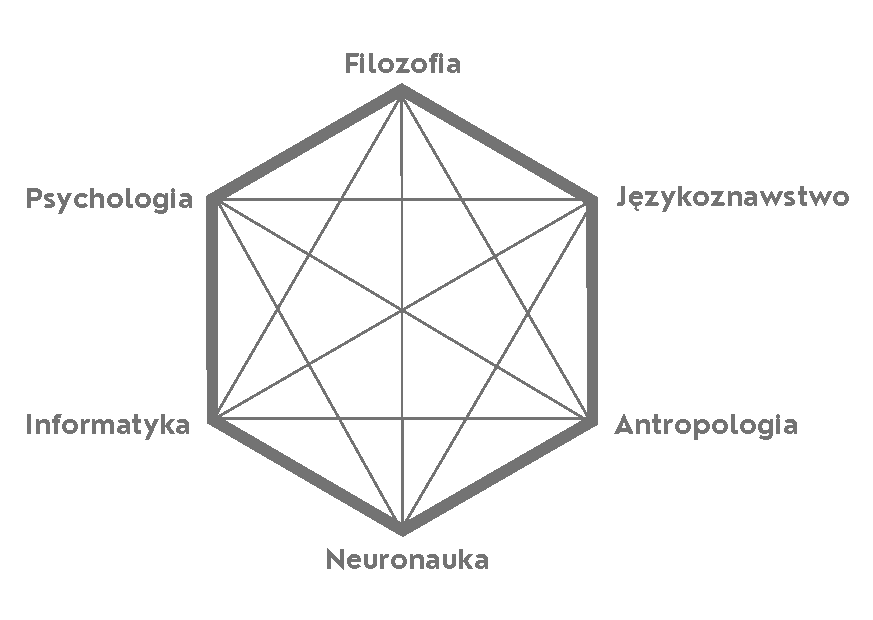
\includegraphics[width=.9\textwidth]{ART_milkowski/ilustracja1pu.pdf}
\end{center}
 \caption{Heksagram obrazujący udział sześciu dyscyplin: językoznawstwa, neurobiologii, sztucznej inteligencji, filozofii, psychologii oraz antropologii w powstawaniu kognitywistyki.}\label{fig1milk}
\end{figure}

Co się jednak stało, że ostatecznie wykluczono rolę społeczeństwa i~kultury z~głównego nurtu kognitywistyki, doprowadzając przy tym do rozejścia się dróg antropologów i~kognitywistów? Za jedną z~przyczyn uważa się rozłam w~samej antropologii na obszar przyrodniczo-\mbox{-ścisły} i~humanistyczny, gdzie antropologia poznawcza, wykazująca cechy obu, okazała się ,,niekochanym dzieckiem'', którym nie zaopiekowało się żadne z~,,rodziców''. Również sama współpraca antropologów z~kognitywistami pozostawiała sporo do życzenia. Tych pierwszych zniechęcały preferowane przez drugich ściśle kontrolowane eksperymenty, prowadzone w~sztucznych warunkach laboratoryjnych, przy niedocenianiu roli kontekstu i~realnych warunków. Kognitywiści z~kolei zarzucali antropologom brak odpowiedniego rygoru badawczego i~nadmierne skupienie na danych jakościowych. James Boster podkreślał, że antropologia, w~odróżnieniu od psychologii w~kognitywistyce, ,,skupia się na treści (nie na procesie), na społecznościach i~kontekstach społecznych (nie na jednostkach), na warunkach naturalnych (nie laboratoryjnych), na uchwytywaniu zjawisk w~świecie rzeczywistym, nawet jeśli wymaga to pewnego złagodzenia rygorów, i~troszczy się o~to, czy zebrane dane faktycznie dowodzą tego, co może się wydawać na pierwszy rzut oka''
%\label{ref:RNDyjHJO3J9ub}(za Bender, i~in., 2010, s.~377; przekład własny).
\parencite[za ][s.~377; przekład własny]{bender_anthropology_2010}. %
 Dodajmy, że do podtrzymania tego stanu rzeczy przyczynili się również kontynuatorzy Newella, eliminując rolę społeczeństwa i~kultury z~projektu formowania jednolitej teorii poznania 
%\label{ref:RNDIkQobHmtSa}(Hutchins, 1995a; Bender, i~in., 2010; Anderson, Lebiere, 2003; Kronenfeld, i~in., 2011).
\parencites[][]{hutchins_cognition_1995}[][]{bender_anthropology_2010}[][]{anderson_newell_2003}[][]{kronenfeld_companion_2011}.%


Jak wskazaliśmy na początku artykułu, bezpośredni udział antropologii w~kognitywistyce utrzymał się zasadniczo w~jednym przypadku: w~rozwijanym od lat osiemdziesiątych XX w. nurcie badań nad poznaniem rozproszonym, którym przewodził Hutchins. Badacz ten, związany z~Wydziałem Kognitywistyki na Uniwersytecie Kalifornijskim w~San Diego, od pierwszych prac zdradzał zainteresowanie związkami między myśleniem, językiem i~kulturą. W~połowie lat siedemdziesiątych XX w. prowadził badania etnograficzne na Wyspach Trobriandzkich w~Papui-Nowej Gwinei, koncentrując się na argumentacji w~sporach publicznych. W~ramach stażu podoktorskiego opracował model tradycyjnej nawigacji mikronezyjskiej, głównie na podstawie dostępnych opracowań praktyk nawigacyjnych. Zatrudniony później przez marynarkę wojenną Stanów Zjednoczonych, wykorzystał spostrzeżenia z~bezpośrednich badań etnograficznych do tworzenia komputerowych systemów szkoleniowych dla układów o~napędzie parowym oraz nawigacji radarowej. Swoje obserwacje poszerzył o~nawigację morską, a~następnie wykorzystał je w~swoim pierwszym, obszernym opracowaniu podstaw teorii poznania rozproszonego, czyli najbardziej docenianej książce \textit{Cognition in the Wild}
%\label{ref:RNDjuIH0R9DmK}(\textit{Hutchins, 1995a}).
\parencite*[][]{hutchins_cognition_1995}. %
 Pod koniec lat osiemdziesiątych XX w. zaczął prowadzić obserwacje w~lotnictwie cywilnym (sam jest dyplomowanym pilotem). Ponadto badania Hutchinsa objęły takie aktywności poznawcze, jak interakcje człowiek–komputer, obliczeniowe symulacje procesów kulturowych, praktyki naukowców, społeczności małp człekokształtnych, a~ostatnio również -- społeczności delfinów\footnote{Tę ewolucję potwierdza również sam badacz w~korespondencji prywatnej, zaznaczając, że wycofywał się (zwłaszcza w~ciągu ostatnich 15 lat) z~agnostycyzmu co do natury procesów mózgowych pod wpływem postępów w~naukach poznawczych -- co powinno być istotne dla tych, którzy traktują \textit{Cognition in the Wild} 
%\label{ref:RND5ANGzGWWK5}(1995a)
\parencite*[][]{hutchins_cognition_1995} %
 jako obowiązującą w~całości po dziś dzień biblię teorii poznania rozproszonego.}.

Będziemy argumentować, że pod względem konceptualizacji systemów i~procesów poznawczych koncepcję poznania rozproszonego można traktować jako swego rodzaju konkurencję dla rozpowszechnionej w~badaniach społecznych teorii aktora-sieci (ANT) Brunona Latoura. Ta ostatnia oferuje ujęcie relacji poznawczych, które zupełnie zrywa z~indywidualizmem metodologicznym -- czego w~kognitywistyce nie zaoferowało żadne inne podejście poza koncepcją poznania rozproszonego
%\label{ref:RND2xoVmWe9Hg}(co wykazano w: Wachowski, 2022).
\parencite[co wykazano w:][]{wachowski_poznanie_2022}. %
 W~przeciwieństwie jednak do ANT, teoria Hutchinsa sprzyja współpracy interdyscyplinarnej, którą Latour dogmatycznie odrzuca. Stanowisko Latoura wydaje nam się o~tyle symptomatyczne, że może świadczyć o~pewnym braku porozumienia między badaczami procesów społecznych i~poznawczych, które prowadzi do stosunkowo małej obecności prac antropologów w~kognitywistyce 
%\label{ref:RNDuRCH2wLhKC}(Núñez, i~in., 2019)
\parencite[][]{nunez_what_2019} %
 i~zbyt ograniczonej, naszym zdaniem, recepcji prac spod znaku poznania rozproszonego w~samej antropologii. Przy tym wszystkim należy podkreślić, że mimo wszystko koncepcja poznania rozproszonego została w~wyraźnej mierze zainspirowana propozycją Latoura 
%\label{ref:RNDurJhglb6K4}(zob. np. Hutchins, 2001).
\parencite[zob. np.][]{hutchins_cognition_2001}.%

\enlargethispage{2\baselineskip}

Interdyscyplinarne badanie procesów poznawczych i~społecznych w~ich wzajemnym powiązaniu jest niewątpliwie o~tyle trudne, że ich badania wymagają kontrolowania bardzo wielu czynników jednocześnie, co jest kłopotliwe szczególnie w~badaniach obserwacyjnych, a~nie eksperymentalnych. Antropologowie i~badacze społecznych procesów wiedzy chcą je zaś często obserwować w~warunkach naturalnych. Propozycja Hutchinsa jednak pozwala połączyć takie obserwacyjne podejście z~rygorem typowym dla kognitywistyki. Daje to szansę na rozwój badań zarówno społecznych, jak i~poznawczych. W~tym przypadku interdyscyplinarność nie tylko wspiera się na argumentach pojęciowych -- takich jak (1) możliwość ugruntowania procesów społecznych w~dobrze rozumianych procesach poznawczych, (2) możliwość teoretycznej unifikacji nauk społecznych przez odwołanie do poznawczych wyjaśnień zachowań racjonalnych, (3) konieczność poprawnego ujęcia poznawczych podstaw procesów społecznych, czy (4) uzupełnianie się kognitywistyki i~socjologii poznawczej
%\label{ref:RNDeNzFI7FeMz}(por. Kaidesoja, i~in., 2019)
\parencite[por.][]{kaidesoja_arguments_2019} %
 -- lecz także na dobrze opracowanej metodologii badawczej. Hutchins jest więc, naszym zdaniem, znakomitym ambasadorem interdyscyplinarnej pracy badawczej na styku nauk społecznych i~poznawczych. Pokazuje nieodzowność i~sposób uwzględniania społecznych determinant rozproszonych procesów poznawczych, a~także kognitywistyczną metodę modelowania tych procesów społecznych.

\section{Teoria, metoda i~przedmiot badań}

Hutchins forsuje projekt włączenia ,,kultury, kontekstu i~historii'' w~sam rdzeń badań nad poznaniem
%\label{ref:RNDu2OUcCpqaH}(Hutchins, 2001, s.~2072).
\parencite[][s.~2072]{hutchins_cognition_2001}. %
 Nie neguje klasycznej metodologii i~dorobku nauk poznawczych, proponuje jednak ich istotne rozszerzenie: metodologiczne i~konceptualne. Przedmiotem jego badań najczęściej są struktury złożone z~ludzi oraz rzeczy (przeważnie artefaktów). Autor \textit{Cognition in the Wild} traktuje ludzkie myślenie jako działalność kulturową. W~tym kontekście można wyróżnić teorię poznania rozproszonego oraz ekologię poznawczą, dominującą w~ostatnich pracach Hutchinsa. Stanowi ona jednak rodzaj szerszej ramy pojęciowej, w~której plasuje między innymi własną teorię.

Celem ekologii poznawczej jest badanie zjawisk poznawczych w~otoczeniu kulturowo-społecznym. Opisuje ona system zależności między procesami poznawczymi a~strukturami grup. Badane zależności dotyczą procesów umysłowych, społecznych i~materialnych oraz ciał. Elementy ekologii poznawczej od dawna bywały sporadycznie obecne w~kognitywistyce. Wraz z~dowartościowaniem kontekstu kulturowo-społecznego poznanie przestaje być postrzegane jako proces racjonalnego wnioskowania logicznego, a~zaczyna być traktowane też jako zjawisko biologiczne. W~ekologii poznawczej wskazuje się na sieć wzajemnych zależności między elementami systemu poznawczego. Znacznej wagi nabiera pytanie o~jednostkę analizy. Hutchins wychodzi od banalnej konstatacji, że wszystko się ze sobą wiąże. Jednak nie każde połączenie jest jednakowo istotne, dzięki czemu badania naukowe pozostają możliwe. Wytyczenie granicy zawsze ułatwia spostrzeżenie jednego, a~utrudnia czy wręcz uniemożliwia -- ujrzenie czegoś innego. Hutchins powołuje się na Gregory'ego Batesona, który podkreślał, że wytyczanie granic jednostek analizy nie powinno pozostawiać ważnych kwestii niewyjaśnionych ani niewyjaśnialnych
%\label{ref:RNDxmKWL5YXAh}(Hutchins, 2008, 2010a).
\parencites{hutchins_cognivite_2008}[][]{hutchins_cognitive_2010}.%


Hutchins wskazuje na trzy ujęcia historycznie ważne dla ekologii poznawczej. Jednym z~nich jest zainicjowana przez Jamesa Gibsona psychologia ekologiczna z~jej teorią afordancji. Gibson jako ,,afordancje'' opisywał właściwości relacyjne ustrukturyzowanego środowiska, prowokujące organizm do określonego, niewymagającego namysłu zachowania. Wbrew Gibsonowi, który odrzuca wyjaśniania odwołujące się do procesów reprezentowania czy obliczania, Hutchins przyjmuje typowe w~kognitywistyce założenia o~obliczeniowo-reprezentacyjnym charakterze poznania. Kolejne ważne tutaj ujęcie to Batesonowska ekologia umysłu, odwołująca się do cybernetycznych sprzężeń i~teorii systemów. Trzecie zaś to kulturowo-historyczna teoria czynności Lwa Wygotskiego. Hutchins widzi ich kontynuację we współczesnych kognitywistycznych teoriach ucieleśnienia, rozszerzenia, ogólniej -- usytuowania poznania, jak również we własnej teorii poznania rozproszonego
%\label{ref:RNDa7odUC3De5}(Hutchins, 2010a, s.~707–712).
\parencite[][s.~707–712]{hutchins_cognitive_2010}.%


Kultura nie stanowi dla tego badacza zbioru rzeczy, materialnych czy abstrakcyjnych, ale proces -- zachodzący wewnątrz i~na zewnątrz ludzkich umysłów -- na który składają się przede wszystkim procesy poznawcze. Jest ona procesem adaptacyjnym, który akumuluje rozwiązania powtarzających się problemów, a~badanie go wymaga oderwania się od myślenia w~kategoriach przyjętych z~góry granic systemów poznawczych. Na ludzki ekosystem składają się różnorodne zasoby poznawcze, do których należą obiekty fizyczne, modele umysłowe, a~także praktyki kulturowe. Zarówno artefakty, jak i~praktyki mają swoje historyczne, kulturowe ścieżki rozwojowe. Ludzkie myślenie Hutchins opisuje jako rodzaj praktyki kulturowej, nabywanej w~toku ucieleśnionych interakcji i~zgodnie z~powszechnymi społecznymi i~materialnymi prawidłowościami oraz znaczeniami obecnymi w~świecie, a~ściślej biorąc, w~kulturowym ekosystemie jednostki ludzkiej, uczącej się nie przez obserwację, lecz poprzez współuczestniczenie. Dla Hutchinsa ów kulturowy ekosystem poznawczy staje się przedmiotem nowej nauki, dzięki której można go lepiej poznać
%\label{ref:RND9rdXUBRnT0}(Hutchins, 1995a, s.~353–355, 2006, 2014).
\parencites[][s.~353–355]{hutchins_cognition_1995}{hutchins_distributed_2006}{hutchins_cultural_2014}.%


Istotnym kulturowo procesem jest materialne osadzanie modeli pojęciowych. Hutchins podaje przykład kolejki w~punkcie usługowym. Praktyka ta stwarza rodzaj przestrzennej pamięci, wprowadzając liniowy porządek umożliwiający zrealizowanie usługi. Nie każdy taki porządek jest kolejką \href{https://www.zotero.org/google-docs/?MOG7xK}{–} mimo zewnętrznego podobieństwa. Praktykę korzystania z~kolejki można postrzegać więc jako poznawczą, bo bez niej obsługa w~kolejności jest trudna. Ma ona w~istocie ponadindywidualne funkcje poznawcze: przede wszystkim umożliwia rejestrowanie i~utrwalanie kolejności przybywających klientów, jak również zarządzanie zapominaniem, gdy ludzie opuszczają kolejkę przed zrealizowaniem swojej potrzeby lub po jej realizacji
%\label{ref:RNDfzSptsM4RE}(Hutchins, 2005, s.~1559–1560, 2014, s.~39–40).
\parencites[][s.~1559–1560]{hutchins_material_2005}[][s.~39–40]{hutchins_cultural_2014}.%


Wszystkie założenia ekologii poznawczej w~ramach kognitywistyki ma uwzględniać teoria poznania rozproszonego. Przyjrzymy się jej, uwzględniając przemiany stanowiska Hutchinsa w~kontekście rozwoju nauk poznawczych, jego kolejne analizy założeń teoretycznych, by wreszcie skonfrontować ją z~koncepcją Brunona Latoura.

Według teorii poznania rozproszonego właściwa jednostka analizy -- przedmiot badań kognitywistycznych i~społecznych -- powinna być ustalana nie \textit{a~priori}, lecz z~uwagi na naturę badanego zjawiska. Owa jednostka, czyli system poznawczy, niekiedy może mieścić się w~granicach czaszki lub skóry człowieka czy innego zwierzęcia, może jednak również wykraczać poza jednostkę, obejmując zarówno żywe, jak i~nieorganiczne składniki, a~więc funkcjonując w~pewnej makroskali
%\label{ref:RNDBky7tQkbeF}(Hutchins, 1995a, s.~128–129, 2001, s.~2068, 2010b, s.~426).
\parencites[][s.~128–129]{hutchins_cognition_1995}[][s.~2068]{hutchins_cognition_2001}[][s.~426]{hutchins_enaction_2010}. %
 Jest to modelowy wręcz przykład zawieszenia indywidualizmu metodologicznego, tak jak rozumie się go w~kognitywistyce, ale i~w filozofii umysłu.

Pojęcie ,,indywidualizm metodologiczny'' jest dość dobrze ugruntowane w~socjologii
%\label{ref:RNDEQWssUHksU}(np. Schumpeter, 1908; Weber, 2002),
\parencites[np.][]{schumpeter_wesen_1908}[][]{weber_gospodarka_2002}, %
 gdzie wyjaśnianie zjawisk społecznych prowadzić ma do ukazania ich jako skutków indywidualnych działań. W~filozofii umysłu i~kognitywistyce jednak pojmowane jest nieco inaczej. Jerry Fodor odróżnił pojęcie indywidualizmu metodologicznego od pojęcia solipsyzmu metodologicznego. Jak twierdzi, według indywidualizmu metodologicznego stany psychiczne indywiduuje się ze względu na ich moce przyczynowe. Zgodnie z~indywidualizmem można więc mówić o~relacjach przyczynowych między podmiotem a~środowiskiem, jeśli są istotne dla stanów psychicznych. Według solipsyzmu metodologicznego zaś stany psychiczne indywiduuje się niezależnie od wartościowania semantycznego (tego, do czego stany te się faktycznie mają odnosić); a~więc pomijane są relacje przyczynowe między podmiotem a~środowiskiem 
%\label{ref:RNDfEZ4x9iWCw}(Fodor, 1980; por. też Heath, 2020).
\parencites[][]{fodor_methodological_1980}[por. też][]{heath_methodological_2020}.%



W~kontekście kognitywistyki przyjmujemy rozumienie indywidualizmu metodologicznego odbiegające nieco od stanowiska bronionego przez Fodora. W~wersji radykalnej oznacza on założenie, że wiedza o~podmiocie poznania (procesach zachodzących w~jego umyśle czy mózgu) jest konieczna i~wystarczająca do zrozumienia procesów poznawczych, wobec czego ignoruje się środowisko podmiotu oraz interakcje z~nim, gdyż nie są one własnościami podmiotu. W~takiej postaci indywidualizm metodologiczny nie jest już może stanowiskiem dominującym w~kognitywistyce. Można wskazać różne stopnie zerwania z~nim czy też zawieszenia go (patrz Ilustracja \ref{fig2milk}), od założenia istotnej roli ciała pozaneuronalnego w~poznaniu, przez rolę środowiska, w~którym podmiot jest poznawczo zakorzeniony, po koncepcje umysłu rozszerzonego czy też szerokiego systemu, w~którym indywidualny podmiot ludzki jest jednym z~komponentów, i~to obok artefaktów%
%\label{ref:RNDM5V78g4iUX}(Wachowski, 2022)
\footnote{Więcej na temat indywidualizmu metodologicznego i~przypadkach zrywania z~nim: \parencite[][]{wachowski_poznanie_2022}.}.


\begin{figure}
\begin{center}
 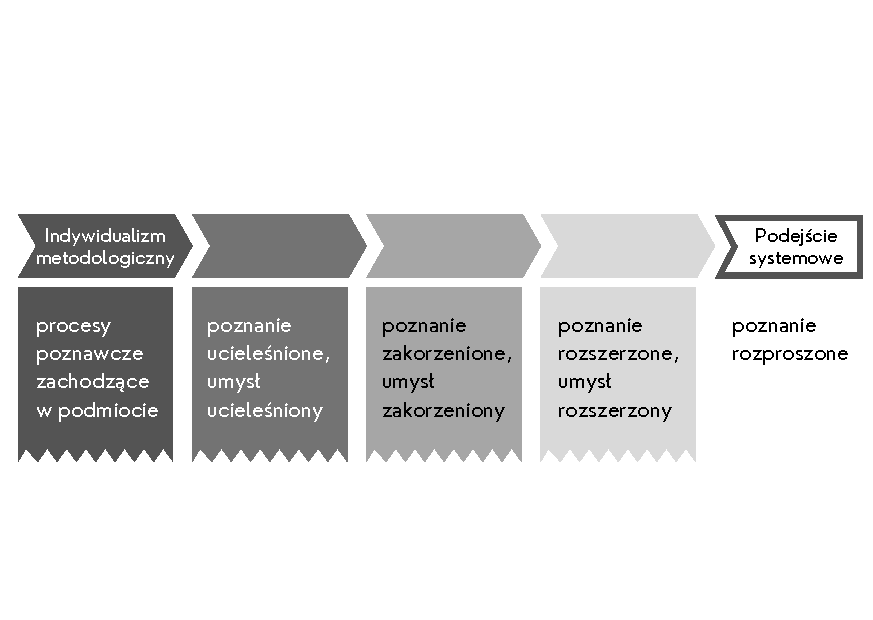
\includegraphics[width=1\textwidth]{ART_milkowski/ilustracja2pu.pdf}
\end{center}
 \caption{Różne stopnie odejścia od indywidualizmu metodologicznego.}\label{fig2milk}
\end{figure}



Dla Hutchinsa każdy taki system jest rozproszonym systemem poznawczym, niezależnie od jego skali -- ta bowiem może ulegać zmianie w~działaniu, a~przez to również przesuwać swoje granice. Poznanie rozproszone nie stanowi żadnego określonego rodzaju poznania, lecz ujęcie bądź sposób badania poznania każdego rodzaju: ,,Dla każdego procesu poznawczego musi istnieć sposób ujęcia go jako rozproszonego''. Dlatego ,,podejście to nie wnosi żadnych twierdzeń o~naturze świata. Jest raczej sposobem patrzenia na ten świat''
%\label{ref:RND1x6mwGwhCQ}(Hutchins, 2014, s.~36).
\parencite[][s.~36]{hutchins_cultural_2014}. %
 W~omawianej teorii właściwe pytania nie dotyczą więc tego, czy dane poznanie jest, czy nie jest rozproszone, ale składników danego systemu i~relacji między nimi, wyłaniania się procesów poznawczych z~interakcji w~systemie itp. Jak podkreśla badacz, perspektywa poznania rozproszonego nie ma żadnych założeń empirycznych. Nie można jej potwierdzić ani obalić. Można natomiast w~jej obrębie stawiać hipotezy empiryczne, między innymi hipotezę umysłu rozszerzonego, którą powinno się móc uzasadnić bądź odrzucić w~trakcie badań empirycznych 
%\label{ref:RNDSfUBAPgJSP}(Hutchins, 2014, s.~36–37).
\parencite[][s.~36–37]{hutchins_cultural_2014}.%


Warto zatem porównać teorię Hutchinsa z~koncepcją umysłu rozszerzonego
%\label{ref:RNDdjlTvhdZZj}(Clark, Chalmers, 2008).
\parencite[][]{clark_umysl_2008}. %
 Koncepcja ta głosi, że granice umysłu nie kończą się na głowie: częścią (a nie tylko narzędziem) umysłu mogą być zewnętrzne wobec układu nerwowego procesy i~przedmioty fizyczne, np. implanty stanowiące dodatkowe receptory zmysłowe, urządzenia obliczeniowe, systemy symboliczne (np. notacja matematyczna) lub nawet całe współpracujące ze sobą grupy. Badacz potwierdza pewne podobieństwa między nimi; podkreśla jednak dwie ważne różnice. Po pierwsze, koncepcja Clarka i~Chalmersa dotyczy tylko pewnego rodzaju poznania: w~jej ujęciu umysł czasami rozszerza się poza granice mózgu, a~czasami nie. Po drugie, w~systemie umysłu rozszerzonego daje się wyróżnić jego centrum (zwykle mózg lub też cały organizm). Dlatego też koncepcję tę można traktować jako dotyczącą szczególnego przypadku funkcjonowania umysłu -- czyli może ona być rozwijana na podstawie szerszych założeń teorii poznania rozproszonego 
%\label{ref:RNDe3LweFYY91}(Hutchins, 2011, s.~437–446, 2014, s.~35–36).
\parencites[][s.~437–446]{hutchins_enculturating_2011}[][s.~35–36]{hutchins_cultural_2014}.%


Hutchins, odrzucając indywidualizm metodologiczny, nie odchodzi od założeń komputacjonistycznych i~reprezentacjonistycznych, gdy określa poznanie jako obliczanie realizowane poprzez wytwarzanie, przetwarzanie i~przekazywanie stanów reprezentacyjnych
%\label{ref:RND4ffDHPRKLP}(Hutchins, 1995a, s.~49).
\parencite[][s.~49]{hutchins_cognition_1995}. %
 Przez ,,stany reprezentacyjne'' rozumie się stany nośników materialnych (zewnętrznych lub np. mózgowych), które oznaczają lub opisują przedmioty procesów poznawczych. Jednak zakres, jaki Hutchins przypisuje poznawczym reprezentacjom i~poznawczym procesom obliczeniowym, zdecydowanie wybiega -- na mocy głównego założenia jego teorii -- poza granice tradycyjnie rozumianych systemów poznawczych. Przedstawiana przez niego perspektywa przypomina nieco punkt widzenia Guliwera, którym byłby psycholog poznawczy, w~krainie olbrzymów: oto otrzymuje on wręcz wymarzoną możliwość bezpośredniej obserwacji procesów przebiegających w~systemie poznawczym w~makroskali, a~więc nie ,,w głowie'', lecz w~otoczeniu, w~które może wejść. Reprezentacje poznawcze stają się więc widzialne i~namacalne: mogą być nimi artefakty. Przez ,,artefakty poznawcze'' teoretycy poznania rozproszonego rozumieją obiekty, które służą do ,,przechowywania, udostępniania lub przetwarzania informacji na potrzeby funkcji reprezentowania, wpływając na poziom wykonania procesów poznawczych u~ludzi'' 
%\label{ref:RNDCkK0TYrHg7}(Norman, 1991, s.~11).
\parencite[][s.~11]{norman_cognitive_1991}. %
 Warto pamiętać, że artefaktami poznawczymi są również gesty czy wypowiedzi. Podobnie dostępne i~obserwowalne jest ich wytwarzanie, przetwarzanie i~przekazywanie, niekiedy dosłownie z~rąk do rąk 
%\label{ref:RND1cj0sn9xl2}(Hutchins, 1995a, s.~128–129).
\parencite[][s.~128–129]{hutchins_cognition_1995}. %
 Tym samym taki makrosystem poznawczy ma własne systemy pamięci zewnętrznej, jak i~mechanizmy oceny i~kontroli sytuacji, z~których żadne nie daje się sprowadzić do pamięci ani aktów oceny i~kontroli indywidualnych podmiotów poznania. Są one natomiast ,,rozproszone'', czy też rozdzielone między ludźmi w~kooperującej grupie lub artefaktami.

Perspektywa poznania rozproszonego to nie po prostu rozwinięcie kognitywistycznej historii o~sprzężeniu podmiotu poznawczego z~otoczeniem. Z~drugiej strony -- powtarzające się odwołania Hutchinsa do obiektów na różnych skalach czasoprzestrzennych, takich jak mózg, układ nerwowy czy ciało jednostkowego podmiotu ludzkiego, dobitnie pokazują, że stanowiska badacza nie można sprowadzać do eksternalistycznych, a~niekiedy wręcz ,,neurofobicznych'', ujęć organizacji systemów rozwiązywania problemów, którego modelowym przykładem miałoby być klasyczne studium nawigacji morskiej. Do takich wniosków mógł prowokować deklarowany przezeń we wcześniejszych pracach częściowy agnostycyzm co do możliwości badania wewnętrznych procesów umysłowych, który z~biegiem czasu coraz bardziej redukował\footnote{Szczegółowa rekonstrukcja w
%\label{ref:RNDc9IGnIMceq}(Afeltowicz, 2012, s.~178–188; Afeltowicz, Wachowski, 2015).
\parencites[][s.~178–188]{afeltowicz_modele_2012}[][]{afeltowicz_how_2015}.%
} -- choć trudno posądzać Hutchinsa o~ignorowanie wagi sprzężenia poznawczego między wewnętrznymi i~zewnętrznymi procesami poznawczymi, o~czym świadczy chociażby wnikliwa analiza funkcjonowania systemu kokpitu samolotu 
%\label{ref:RNDtxxt2Fkllo}(zob. Hutchins, 1995b; Hutchins, Klausen, 1996).
\parencites[zob.][]{hutchins_how_1995}[][]{engestrom_distributed_1996}. %
 Z~drugiej strony nie brakowało wyważonych ujęć jego teorii również we wcześniejszym okresie, jak chociażby autorstwa Yvonne Rogers 
%\label{ref:RND4byZChM8wV}(1997)
\parencite*[][]{rogers_brief_1997} %
 czy też takich współpracowników Hutchinsa, jak David Kirsh 
%\label{ref:RNDBuTbdSizkw}(1999).
\parencite*[][]{kirsh_distributed_1999}. %
 Jednak nie bez znaczenia są też odniesienia do koncepcji Latoura, przeciwnika uwzględniania jednostkowej psychologii w~wyjaśnianiach funkcjonowania kolektywnych struktur poznawczych, jak również twórcy podejścia metodologicznego, kojarzonego z~podejściem reprezentantów nurtu społecznych badań nad nauką i~techniką 
%\label{ref:RNDoko8d9fvmf}(zob. np. Hess, 2001).
\parencite[zob. np.][]{hess_ethnography_2001}.%


Główna metoda badawcza Hutchinsa jest etnograficzna. W~metodach etnograficznych docenia Hutchins możliwość badań nad rzeczywistym poznaniem w~rzeczywistym świecie, pozwalającą na wyprowadzenie ich poza ograniczoną przestrzeń laboratorium
%\label{ref:RNDwjlRdGES2W}(Hutchins, 2014, s.~43).
\parencite[][s.~43]{hutchins_cultural_2014}. %
 Takie podejście, zastosowane do procesów poznawczych, wydaje się w~pełni legitymizować odejście od indywidualizmu metodologicznego, nie tak oczywiste w~kognitywistyce. Jakościowa metoda etnograficznych badań poznawczych wykorzystuje obserwacje funkcjonowania danej wspólnoty do analiz jej aktywności poznawczej.

Różnicę między etnografią tradycyjną a~poznawczą można za Robertem Williamsem określić następująco: podczas gdy pierwsza zajmuje się znaczeniami wytwarzanymi przez członków danej wspólnoty kulturowej, druga koncentruje się na tym, jak te znaczenia są przez nich wytwarzane. Etnografowie tradycyjni wskazują materialne i~konceptualne zasoby składające się na lokalną rzeczywistość danej grupy, etnografowie kognitywni badają sposób, w~jaki te zasoby są wykorzystywane w~aktywności kulturowej. Pierwsi analizują myślenie ludzi definiujące ich grupę kulturową, natomiast drudzy obserwują sam ten proces; pierwsi opisują wiedzę, a~drudzy -- procesy konstrukcji i~wykorzystywania wiedzy. Oczywiście różnice te nie świadczą o~istnieniu między nimi przepaści
%\label{ref:RNDTBswyeN3Lq}(Williams, 2006, s.~838).
\parencite[][s.~838]{williams_using_2006}.%


Co tutaj istotne, zainteresowanie procesami poznawczymi funkcjonującymi w~środowisku naturalnym (tytułowe \textit{in the wild}) nie oznacza, że dla Huchinsa procesy przebiegające w~warunkach laboratoryjnych są nienaturalne i~niegodne badania lub że wręcz stoją poza kulturą. Nic bardziej błędnego: poznanie nie zna próżni kulturowej, więc miejsca, w~których przeprowadza się wyizolowane eksperymenty, nie mogą stanowić tutaj wyjątku. Obserwacje etnograficzne w~laboratoriach są po prostu trudniejsze, bo aspekty kulturowe pozostają tam niejako przezroczyste, co wymaga po prostu szczególnego podejścia badawczego
%\label{ref:RND3JRJN8V6Nn}(Hutchins, 1996, s.~66–67).
\parencite[][s.~66–67]{hutchins_response_1996}. %
 Że są możliwe i~interesujące, sam Hutchins udowadnia między innymi we współautorskim studium etnograficznym aktywności neurobadaczy 
%\label{ref:RNDkeP7sxcfO1}(Alač, Hutchins, 2004).
\parencite[][]{alac_i_2004}.%


Przedmiotem badań nad poznaniem rozproszonym ma być ,,natura poznania'' w~różnego rodzaju systemach działalności. W~badaniach Hutchinsa były one dość różnorodne, a~więc kultura Wysp Trobriandzkich, systemy nawigacji i~awiacji, społeczności małp człekokształtnych oraz delfinów, systemy interakcji człowiek-komputer (HCI), wspólnoty naukowców, jak również grupy realizujące tak codzienne praktyki kulturowe, jak opisana już kolejka. Poza obserwacjami \textit{in the wild} badacz ten przeprowadzał również obliczeniowe symulacje procesów kulturowych. Wskazując przy tym na różne skale realnych rozproszonych systemów poznawczych, plasuje on umysł rozszerzony na średnim poziomie skali, podkreślając, że w~systemie tego typu mamy do czynienia z~centralizacją poznawczą
%\label{ref:RNDYENpyx0zDM}(Hutchins, 2014, s.~37).
\parencite[][s.~37]{hutchins_cultural_2014}. %
 Systemami pozbawionymi takiej centralizacji byłyby już takie funkcjonalne struktury człowiek-artefakt, jak kokpity pojazdów, laboratoria, instytucje finansowe czy internet. Istnieją także rozległe i~różnorodne przestrzenie inteligencji zbiorowej, gdzie jednostkami systemu są samodzielne, aktywne podmioty poznania. Tutaj przykładem mogą być społeczności owadów, rynki ekonomiczne oraz media społecznościowe 
%\label{ref:RNDo452cepHYt}(Hutchins, 2014, s.~37).
\parencite[][s.~37]{hutchins_cultural_2014}.%


Przyjrzyjmy się najbardziej znanemu Hutchinsowskiemu studium przypadku, jakim były czteromiesięczne badania etnograficzne na początku lat dziewięćdziesiątych XX w. nad nawigacją morską na pokładzie amerykańskiego lotniskowca\footnote{Literatura przedmiotu obejmuje również prace poświęcone poznaniu rozproszonemu społecznie, które można by traktować jako pewnego rodzaju formę przejściową w~stosunku do analiz heterogenicznych struktur dokonywanych przez Hutchinsa
%\label{ref:RND7tkMcbcoey}(Roberts, 1964; Salomon, 1993).
\parencites[][]{roberts_self-management_1964}[][]{salomon_distributed_1993}. %
 }. Zespół marynarzy i~oficerów musi odpowiedzieć na prosto brzmiące pytanie: ,,gdzie jesteśmy i~dokąd zmierzamy?'', stawiane oczywiście z~perspektywy osób przebywających na pokładzie statku. Zapomnijmy tutaj na moment o~GPS i~systemach satelitarnych, ponieważ dopiero zaczynano je wdrażać i~były jeszcze dość zawodne.

Aby dokładnie wytyczyć położenie statku, nawigatorzy muszą dysponować co najmniej trzema łukami pozycyjnymi (AOP), wyznaczanymi na podstawie odległości do określonego punktu orientacyjnego, bądź liniami pozycyjnymi (LOP), wyznaczanymi na podstawie mierzonego w~stopniach położenia okrętu względem widocznego punktu orientacyjnego. Owe łuki i~linie oznaczane są na mapie cyrklem oraz specjalnym kątomierzem. Natomiast wyznaczanie LOP odbywa się z~wykorzystaniem pelorusów, czyli specjalnych urządzeń przypominających kompasy bez igły, umieszczonych na burcie lub pokładzie, dzięki którym obsługujący je marynarze wyszukują punkt obserwacyjny i~w żądanym momencie podają kwatermistrzowi odczyt z~tarczy. Najważniejszym przyrządem -- określanym przez Hutchinsa jako analogowy komputer -- jest mapa rozłożona w~kabinie nawigacyjnej, gdyż to wokół niej koncentrują się działania nawigatorów. Reprezentując przestrzeń geograficzną, daje ona nawigatorom unikatową perspektywę. Ponadto jednak mapa nawigacyjna stanowi urządzenie obliczeniowe: dzięki niej zachodzi zewnętrzne obliczanie, niemające odpowiednika w~niczyjej obecnej tam głowie, nawet oficerów. Odpowiedzi na zadawane pytania nawigatorzy otrzymują, wykonując proste czynności takie jak obsługa cyrkla i~kątomierza, rysowanie linii czy przepisywanie cyfr. Cała procedura stanowi, zdaniem Hutchinsa, doskonałą ilustrację Latourowego myślenia za pomocą rąk i~oczu
%\label{ref:RNDMaCVn4m2rV}(Hutchins, 1995a, s.~142–143).
\parencite[][s.~142–143]{hutchins_cognition_1995}. %
 W~tym kontekście Hutchins przytacza słowa Herberta Simona: ,,rozwiązanie problemu to po prostu przedstawienie go w~taki sposób, aby rozwiązanie stało się oczywiste'' 
%\label{ref:RNDHN1L3EqIMz}(Hutchins, 1995a, s.~117).
\parencite[][s.~117]{hutchins_cognition_1995}.%


Mapa nawigacyjna pełni kilka ważnych funkcji. Stanowi podstawową reprezentację zewnętrzną, umożliwiającą przeprowadzanie obliczeń. Pozwala na integrowanie i~porównywanie informacji pochodzących z~różnych źródeł. Służy do koordynacji ludzkich działań. Stanowi także środek monitorowania jakości pracy nawigatorów. Przy tym wszystkim jest zewnętrznym systemem pamięci (zresztą przechowywanym pieczołowicie i~w kilku kopiach), obejmującym wiedzę (wraz z~jej modyfikacjami) zarówno członków danej załogi okrętu, jak i~różnych pokoleń marynarzy, badaczy, geografów, kartografów
%\label{ref:RNDKwGI4POv2k}(Afeltowicz, Wachowski, 2015, s.~93–98; Hutchins, 1995a, s.~61–143).
\parencites[][s.~93–98]{afeltowicz_how_2015}[][s.~61–143]{hutchins_cognition_1995}.%


\section{Korzenie, inspiracje, interpretacje}

Do jakiego stopnia mamy tutaj do czynienia z~nową propozycją teoretyczną? Jak się mają te badania nad poznaniem do reszty nauk poznawczych? Odpowiedzi na oba te ważne pytania wiążą się ze sobą, a~wstępną odpowiedź naszkicowaliśmy już wcześniej, omawiając ekologię poznawczą.

Osbeck i~Nersessian
%\label{ref:RNDJbap64ket5}(2014),
\parencite*[][]{osbeck_situating_2014}, %
 podejmując własną próbę historycznego usytuowania teorii poznania rozproszonego, wskazują na analogie z~psychologią funkcjonalną -- w~tym stanowiskami Williama Jamesa i~Johna Deweya -- jednocześnie sugerując związki teoretyczne z~pragmatyzmem filozoficznym. Funkcjonaliści podejmowali ,,problem kontekstu'', ujmując działający podmiot w~,,pełnej'' sytuacji, jego życie umysłowe jako proces adaptacyjny, a~procesy poznawcze raczej jako pewną aktywność niż nabywanie wiedzy. Porównując psychologię funkcjonalną i~teorię poznania rozproszonego, Osbeck i~Nersessian wskazują na zbieżności: perspektywa systemowa i~dynamiczna, nacisk na rozwiązywanie problemów, sprzeciw wobec czysto intelektualnej wizji poznania, oddzielonego od świata rzeczy i~zjawisk społecznych, preferowanie badań nad zjawiskami zachodzącymi w~rzeczywistym (a nie sztucznym, laboratoryjnym) środowisku.

Na uwagę zasługują wpływy i~zbieżności z~perspektywą radzieckiej szkoły kulturowo-historycznej Lwa Wygotskiego i~Aleksandra Łurii. Ten ostatni, komentując stanowisko Wygotskiego
%\label{ref:RND34bUoj8PY6}(np. Vygotskij, 1971; warto także porównać z: Mead, 1975),
\parencites[np.][]{vygotskij_wybrane_1971}[warto także porównać z:][]{mead_umysl_1975}, %
 wywodzącego indywidualne akty psychiczne z~zachowań grupowych, stwierdzał, że jeśli mamy wyjaśnić złożone formy ludzkiej świadomości, powinniśmy w~analizach wyjść poza granice organizmu, w~sferę zewnętrznych warunków jego życia, uwzględniając tak społeczny, jak i~historyczny ich wymiar 
%\label{ref:RNDaAnLjhFbmJ}(Luriâ, 1979).
\parencite[][]{luria_azyk_1979}. %
 Michael Cole i~Yrjö Engeström wymieniają następujące elementy podejścia kulturowo-historycznego, które można traktować jako początki teorii poznania rozproszonego: zasady rządzące ,,naturalnymi'' psychicznymi czynnościami człowieka są różne od zasad rządzących jego czynnościami ,,kulturowymi'' -- upośrednionymi przez narzędzia i~normy społeczne; to kulturowe upośrednienie kształtuje szczególnego rodzaju strukturę ludzkiego umysłu i~zachowania, modyfikując podmiot i~jednocześnie jego otoczenie; interakcję między nimi regulują kulturowe artefakty, zarówno materialne, jak i~symboliczne. Niezwykle ważnym narzędziem tego upośrednienia jest język. W~danym otoczeniu kulturowym skumulowana jest również wiedza poprzednich pokoleń, dlatego w~rozwoju osobniczym ważną rolę odgrywa środowisko społeczne. Stąd też naturalną jednostką analizy w~badaniach nad ludzkim zachowaniem stają się systemy czynności, rozumiane jako historycznie uwarunkowane systemy relacji między jednostkami ludzkimi a~ich najbliższym, kulturowo ustrukturyzowanym otoczeniem. Autorzy zestawiają wyniki prac radzieckich psychologów nurtu kulturowo-historycznego z~wnioskami wspomnianego już Deweya, ale także Wilhelma Wundta i~Hugo Münsterberga, dostrzegając w~nich zbliżone sposoby konceptualizacji poznania jako zjawiska rozproszonego, w~ramach których dochodzi do zjednoczenia nauk przyrodniczych i~kulturowych 
%\label{ref:RNDxtyiUJ6lJK}(Cole, Engeström, 1993).
\parencite[][]{cole_cultural-historical_1993}.%


Dysponujemy już pewną wiedzą o~stosunkowym nowatorstwie teorii Hutchinsa, powróćmy więc do pytania o~to, jak ma się ona do szerszego dorobku nauk poznawczych. O~stopniu osadzenia teorii poznania rozproszonego w~klasycznej kognitywistyce dobre pojęcie daje książka \textit{Cognition in the Wild}. Uwidacznia się to między innymi w~specyficznym rozumieniu obliczania i~reprezentacji: choć sama przyjmowana przez tego autora definicja poznania -- czyli (przypomnijmy) obliczania realizowanego poprzez wytwarzanie, przetwarzanie i~przekazywanie stanów reprezentacyjnych -- bezkolizyjnie łączy omawianą perspektywę z~klasycznymi podejściami w~naukach poznawczych, to wątpliwości pojawiają się co do zakresu, jaki Hutchins przypisuje pojęciom reprezentacji oraz procesom obliczeniowym. Trudno bowiem uznać reprezentacje zewnętrzne (znaki, ilustracje czy gesty) za po prostu równoważne wewnętrznym reprezentacjom umysłowym. Podobnie brakuje powszechnej zgody na to, by uznać zbiorową czynność kolektywu współpracującego przy rozwiązywaniu wspólnego problemu, za czynność poznawczą.

Autor \textit{Cognition in the Wild} wskazuje na pewne nieporozumienia związane z~pojęciami stosowanymi w~kognitywistyce, a~także postuluje reinterpretację jej historii. U~podstaw nieporozumień -- historycznie wzmocnionych -- leży, jego zdaniem, podstawowe niezrozumienie podobieństw i~różnic między komputerami a~umysłami.

Dla Hutchinsa idea procesu obliczeniowego jest podstawowa nie tylko dla poznania, lecz także kultury; opanowanie systemów formalnych to wręcz klucz do rozumienia nowoczesnej cywilizacji
%\label{ref:RNDLR48tqgRIS}(Hutchins, 1995a, s.~359–360).
\parencite[][s.~359–360]{hutchins_cognition_1995}. %
 Jednak to nie umysł ludzki, ile większy wycinek ludzkiego świata kulturowego miałby być komputerem: ,,Architektura systemu fizycznych symboli nie stanowi modelu indywidualnego poznania, ale model działania systemu społeczno-kulturowego, z~którego usunięto indywidualny ludzki podmiot'' 
%\label{ref:RNDP3BxoM3qkK}(Hutchins, 1995a, s.~363).
\parencite[][s.~363]{hutchins_cognition_1995}. %
 Analogicznie Hutchins traktuje system Searle'owskiego chińskiego pokoju jako społeczno-kulturowy system poznawczy, którego właściwości wykraczają poza możliwości poznawcze ludzkiej jednostki. Searle przedstawia następujący eksperyment myślowy 
%\label{ref:RNDw5VUtfF02C}(Searle, 1995).
\parencite[][]{searle_umysly_1995}. %
 W~pewnym pomieszczeniu -- zwanym ,,chińskim pokojem'' -- znajduje się człowiek, posługujący się skomplikowanym podręcznikiem przekładu z~języka chińskiego na angielski. Sam jednak w~ogóle nie zna chińskiego. Przez otwór do pokoju dostaje pytanie w~języku chińskim. Korzystając z~angielskiego podręcznika i~wertując go, odpowiada na pytanie, też po chińsku. Czy powiedzielibyśmy, że rozumie po chińsku? Nie! Dlatego też, powiada Searle, nie ma podstaw, aby przypisywać komputerom rozumienie języka naturalnego. Searle jednak nie rozpoznaje złożoności rozproszonego systemu poznawczego, który sam opisuje w~swoim eksperymencie myślowym. Podobnie, zgodnie z~fałszywą (zdaniem Hutchinsa) ideą, że komputer wykonany jest na obraz i~podobieństwo człowieka, dziesiątki lat historii kognitywistyki można postrzegać jako dążenie do przerobienia obrazu człowieka na obraz komputera 
%\label{ref:RNDkYZeMM4ccG}(Hutchins, 1995a, s.~361–363).
\parencite[][s.~361–363]{hutchins_cognition_1995}. %
 Przy takim podejściu ciało, emocje, kultura musiały stać się elementami dodanymi, uwzględnianymi dopiero na późniejszym etapie dociekań.

Autor \textit{Cognition in the Wild} zakłada, że ludzie rzeczywiście przetwarzają wewnętrzne reprezentacje symboli. Ale nie wierzy w~to, by to manipulacja symbolami stanowiła istotę indywidualnego poznania. Pylyshynowi, który opisuje manipulowanie symbolami zakodowanymi w~koralikach liczydła
%\label{ref:RNDMFKcdNi2s5}(Pylyshyn, 1989, s.~56),
\parencite[][s.~56]{pylyshyn_computing_1989}, %
 Hutchins zarzuca zignorowanie tego, co robi liczący, abstrahowanie od funkcji jego rąk i~oczu, od istoty samego uczenia się, na rzecz skupienia się na właściwościach systemu, który wyłania się dzięki aktywności osoby manipulującej koralikami. Oczywiście Pylyshyn dobrze opisuje obliczeniowe właściwości systemu społeczno-kulturowego, lecz nie aktywność poznawczą podmiotu ludzkiego. Hutchins domaga się podejścia ucieleśnionego, to znaczy uwzględniającego konkretny, fizyczny udział osobnika w~czynnościach liczenia i~uczenia się, gdyż dopiero wtedy można mówić o~jego użytkowaniu przyrządu do rozwiązywania problemów oraz o~nabywaniu określonych umiejętności. W~tych dociekaniach konieczne jest usytuowanie podmiotu poznającego w~realnym świecie. Hutchins przyznaje, że klasyczni zwolennicy hipotezy \textit{systemu fizycznych symboli} są tego świadomi. Allen Newell i~Herbert Simon potwierdzają istotność tak zwanych pamięci zewnętrznych -- a~więc materialnych zasobów dostępnych w~otoczeniu podmiotu rozwiązującego dany problem poznawczy i~wykorzystywanych przezeń równolegle z~pamięcią wewnętrzną 
%\label{ref:RNDBqDSyMdOeS}(Newell, Simon, 1972, s.~800–803).
\parencite[][s.~800–803]{newell_human_1972}. %
 Badacz dostrzega dobry punkt wyjścia, zauważa jednak, że przez dziesiątki lat od wydania przytaczanej tu książki Newella i~Simona wykorzystanie materialnych struktur otoczenia w~procesach poznawczych jakoś nie interesowało głównego nurtu kognitywistyki 
%\label{ref:RNDcRwZJasC4s}(Dahlbäck, Kristiansson, 2016; Hutchins, 1995a, s.~364–370).
\parencites[][]{dahlback_perspective_2016}[][s.~364–370]{hutchins_cognition_1995}.%


Badania Hutchinsa wpisują się w~dosyć swoiście pojmowaną naturalizację badań społecznych -- a~mianowicie pozwalają spełnić wymóg naturalizmu metodologicznego, głoszący, że w~badaniach empirycznych
%metody badawcze
dopuszczalne są wszystkie i~tylko te metody, które są typowe dla nauk przyrodniczych. Za taką naukę przyrodniczą uchodzić ma, rzecz jasna, antropologia kognitywna, integrująca się również z~pozostałymi elementami konglomeratu kognitywistycznego, w~tym także do pewnego stopnia z~neuronauką w~ramach neuroantropologii
%\label{ref:RNDmCjTTYm6pd}(Lende, Downey, 2012).
\parencite[][]{lende_encultured_2012}. %
 Jest tak dlatego, że Hutchins bardzo swoiście rozumie też antropologię poznawczą: jest ona mianowicie badaniem kultury metodami, które proponowano do wyjaśniania procesów rozwiązywania problemów w~psychologii poznawczej. Te wyjaśnienia odwołują się m.in. do operowania symbolami.

Hutchins odwołuje się do bardzo wpływowej propozycji metodologicznej, sformułowanej przez Davida Marra
%\label{ref:RNDytVMerjGC8}(1982),
\parencite*[][]{marr_vision_1982}, %
 a~powszechnie przyjmowanej w~badaniach kognitywistycznych. Marr uważał, że systemy obliczeniowe należy wyjaśniać na trzech poziomach ich realizacji, ponieważ dopiero wyjaśnienie wszystkich poziomów jest kompletne i~satysfakcjonujące. Przede wszystkim należy wiedzieć, jakie zadanie -- opisywane w~kategoriach przetwarzania informacji -- realizuje dany system i~dlaczego realizacja tego zadania jest właściwa w~danym otoczeniu. Ten poziom Marr zwał ,,obliczeniowym'', lecz jest to termin nieco mylący; inni stosowali określenia ,,poziom wiedzy'' 
%\label{ref:RND3bcrtgwcDH}(Newell, 1981)
\parencite[][]{newell_knowledge_1981} %
 ,,poziom semantyczny'' 
%\label{ref:RNDor3Z8HGaA2}(Pylyshyn, 1984)
\parencite[][]{pylyshyn_computation_1984} %
 lub ,,ekologiczny'' 
%\label{ref:RNDHJjKtYSxCi}(Sterelny, 1990).
\parencite[][]{sterelny_representational_1990}. %
 W~przypadku określenia położenia statku wejściowe informacje dostępne są z~wielu, często dających rozbieżne wyniki, przyrządów pomiarowych, których obsługa wymaga współdziałania wielu osób. Rozwiązaniem ma być niezbędna w~żegludze para współrzędnych nałożona na mapę.

Na drugim poziomie -- kluczowym dla Marra -- opisuje się algorytmy i~reprezentacje, na których owe algorytmy pracują. Innymi słowy, opisuje się system obliczeniowy jako urzeczywistniający precyzyjnie opisane procesy przetwarzania informacji, których postać jest dokładnie określona. Tu Hutchins abstrakcyjnie opisuje strukturę systemu -- odzwierciedlającą podział pracy poznawczej -- i~poszczególne składowe reprezentacje oraz kanały przesyłania informacji (np. telefon na pokładzie).

Na trzecim zaś poziomie Marr domaga się wskazania realizacji sprzętowej danego systemu obliczeniowego. Hutchins wskazuje w~szczególności na ograniczenia materialne interakcji społecznej, dzięki którym działania są lepiej koordynowane, a~sekwencja działań mająca prowadzić do ustalenia położenia w~danym momencie jest wykonywana bez zakłóceń. Pozostaje on w~dużej mierze neutralny w~sprawie tego, jak mają się działania poszczególnych osób, będących częściami dużego, rozproszonego systemu poznawczego, do ich indywidualnych zdolności poznawczych. Uważa, że właściwe wyjaśnienie systemu rozproszonego nie musi schodzić na taki niższy poziom, a~zjawisko można wyjaśnić trafnie na bardziej abstrakcyjnym poziomie opisu struktury społeczno-kulturowej wraz z~jej materialną realizacją.

Przy takim podejściu widać od razu, że Hutchins korzysta z~narzędzia, które pozwala mu modelować podział pracy poznawczej, i~to także z~uwzględnieniem skuteczności tej pracy. W~tym miejscu tematyka jego prac wprost łączy się z~klasycznym wątkiem badań socjologicznych, a~metoda badawcza -- opis antropologiczny -- zbliża go do badań społecznych prowadzonych w~mikroskali, lecz jednocześnie metodami umożliwiającymi matematyzację. Tu Hutchins różni się też od innych antropologów poznawczych, którzy, w~odróżnieniu od większości kognitywistów korzystających w~ogromnej mierze z~modelowania obliczeniowego, rzadko odwołują się do symulacji komputerowych, a~prawie nigdy nie przeprowadzają symulacji realnych procesów społeczno-poznawczych w~celu ich wyjaśniania i~przewidywania.

Hutchins między innymi opracował symulacje zjawiska zwanego ,,błędem potwierdzania''. Polega ono na tym, że skłonni jesteśmy uznawać za prawdziwą tę informację, która potwierdzałyby wcześniejsze założenia lub oczekiwania. Badacz pokazał, że zjawisko to może zachodzić w~grupie w~formie procesu rozproszonego; wykorzystał w~tym celu sieć koneksjonistyczną zwaną ,,siecią spełniania ograniczeń'', uzyskując uproszczony model grupowej interakcji. Przy okazji zaobserwował, że błąd potwierdzania zachodzi tym słabiej, im większa jest komunikacja (interakcja) między jednostkami w~sieci
%\label{ref:RNDHhYhoRT1qF}(Hutchins, 1995a, s.~239–255).
\parencite[][s.~239–255]{hutchins_cognition_1995}.%


Podział pracy poznawczej stanowi istotę działania wielu organizacji i~instytucji społecznych, a~próby udoskonalenia ich działania -- jeśli same nie adaptują się do otoczenia -- mogą z~pewnością skorzystać z~bardziej kognitywnego podejścia. Dzięki zastosowanemu tutaj podejściu Hutchinsa można opisać przebieg procesu przetwarzania informacji i~przeanalizować jego efektywność ze względu na założony cel poznawczy. Możliwa jest więc poznawcza analiza społecznych procesów podejmowania decyzji, tak politycznych, jak i~naukowych czy potocznych.

Nie oznacza to wszelako, że metoda obrana przez Hutchinsa jest idealna. Metodologia Marra została opisana przezeń jedynie we wstępie metodologicznym do jego wpływowej książki i~nie odzwierciedla zacierania się granic między kognitywistyką a~neurokognitywistyką, a~także między badaniem procesów kulturowych i~poznawczych. Badacze interesują się bowiem często tym, jakie mechanizmy odpowiadają za procesy psychiczne i~starają się zawęzić swoje hipotezy, odwołując się do świadectw neurobiologicznych czy kulturowych. Marr, \textit{notabene}, też tak czynił, kiedy zwracał uwagę na rozłączne pojawianie się pewnych zaburzeń poznawczych przy ogniskowych uszkodzeniach mózgu. Jednak co do zasady uważał, że nie jest to bynajmniej konieczny element metody wyjaśniania, a~jego opis poziomu realizacji sprzętowej (neuronalnej) pozostaje, podobnie nieco jak i~u~Hutchinsa, osobliwie nieprecyzyjny.

Skupienie się Hutchinsa na budowie i~morfologii systemów poznawczych na różnych poziomach ich podsystemów, a~przez to na udziale artefaktów w~ludzkich procesach poznawczych oraz ogólnie funkcjonowaniu ekosystemów kulturowych, wykazuje duży związek z~pracami Donalda Normana, zwłaszcza z~książką \textit{Things that Make us Smart}
%\label{ref:RNDMIEchfVLok}(1993).
\parencite*[][]{salomon_distributed_1993}. %
 Pojawia się w~niej zresztą pojęcie i~wyjaśnienie poznania rozproszonego oraz wyników badań Hutchinsa jeszcze przed publikacją \textit{Cognition in the Wild}.

Miejsce i~recepcja Normana w~kognitywistyce wymaga kilku słów wyjaśnienia. Ten amerykański kognitywista i~teoretyk wzornictwa przemysłowego, a~jednocześnie najbardziej chyba wpływowy badacz interakcji człowiek-komputer (HCI), jak i~szerzej: człowiek–artefakt, uprawia swoistą inżynierię poznawczą. Zainteresowany jest nie tyle rozwijaniem teorii znanych już interakcji człowiek–artefakt, ile projektowaniem tych interakcji, ich kulturowym zastosowaniem (i tym samym badaniem przez projektowanie). To nastawienie bardzo dobrze współgra z~równie praktyczną orientacją Hutchinsa, konsekwentnie odwołującego się do kulturowego wykorzystywania rzeczy.

\section{Szkodliwe moratorium}

Perspektywą najbardziej zbliżoną do perspektywy Hutchinsa jest nurt społecznych badań nad nauką i~techniką, reprezentowany między innymi przez Brunona Latoura, do którego prac Hutchins zresztą wyraźnie się odwoływał.

W~klasycznych naukach nad poznaniem i~mózgiem zagadnienia społeczne w~poznaniu sprowadza się zasadniczo do procesu społecznego wiązanego z~nabywaniem i~przetwarzaniem informacji o~innych ludziach, komunikowaniem się, empatią. Ścieżka analizy wiedzie tutaj od jednostkowych umysłów czy mózgów do społeczeństwa
%\label{ref:RND8XdzRJeEgZ}(zob. np. Fiske, Taylor, 2008).
\parencite[zob. np.][]{fiske_social_2008}.%


Tymczasem -- jak pokazują Ronald Giere i~Barton Moffatt -- perspektywa naukoznawcza ukazuje wspomnianą relację jako opozycję, w~pewnych przypadkach wskazując na dominację wymiaru społecznego, co byłoby pokłosiem socjologii wiedzy
%\label{ref:RNDGHooPYkgJU}(zob. także Brown, 2011; Giere, Moffatt, 2003, s.~301–302).
\parencites[zob. także][]{brown_science_2011}[][s.~301–302]{giere_distributed_2003}. %
 Wyzywającą manifestacją tej dominacji było dziesięcioletnie moratorium na odwoływanie się do umysłu w~wyjaśnianiu sukcesu nauki, które zaproponował Latour ze Steve'em Woolgarem. Rzucali oni wyzwanie kognitywistyce wyjaśniającej efektywność nauki przez odwołanie do umysłu, ujmowanego jeszcze w~sposób odcieleśniony i~oderwany od kontekstu społecznego i~materialnego: ,,My zaś w~tym miejscu obiecujemy, że jeśli pod koniec tego okresu zostanie cokolwiek [związanego z~poznaniem naukowym] do wyjaśnienia, to my także zwrócimy się w~stronę umysłu!'' 
%\label{ref:RNDQ8MYVWAXEp}(Latour, Woolgar, 2020, s.~366).
\parencite[][s.~366]{latour_zycie_2020}.%


W~badaniach nad poznaniem naukowym Hutchins wydawałby się doskonałym partnerem Latoura; wszak analizował czynności badaczy w~laboratorium neuronaukowym
%\label{ref:RNDq7az7dkeo7}(Alač, Hutchins, 2004).
\parencite[][]{alac_i_2004}. %
 Jego uwagi dotyczące wizualizacji naukowych wpisują się w~perspektywę Latoura 
%\label{ref:RNDQ0asW0EmjX}(np. Latour, 2012).
\parencite[np.][]{latour_wizualizacja_2012}. %
 Prześledźmy ich pouczający spór 
%\label{ref:RNDmhrfwswWJZ}(Latour, 1996; Hutchins, 1996).
\parencites[][]{latour_cogito_1996}[][]{engestrom_distributed_1996}.%


Latour jest badaczem społecznym i~filozofem nauki, kojarzonym z~konstruktywistyczną teorią aktora-sieci (ANT), która przypisuje sprawczość czynnikom ludzkim i~pozaludzkim, znajdującym się w~zmiennych (czasowo wzmacnianych lub też słabnących) sieciach relacji
%\label{ref:RND7AXCpLIIYs}(zob. np. Latour, 2010).
\parencite[zob. np.][]{latour_splatajac_2010}. %
 ,,W szesnastym wieku nie pojawił się żaden nowy człowiek, a~we współczesnych laboratoriach nie pracują wcale mutanci o~rozrośniętych mózgach'' -- stwierdza, namawiając do szukania przyczyn spektakularnych sukcesów nauki w~praktykach i~narzędziach badaczy 
%\label{ref:RNDPXBhMczGqs}(Latour, 2012, s.~208).
\parencite[][s.~208]{latour_wizualizacja_2012}. %
 Analogicznie Hutchins -- co nie uszło uwadze Latoura -- każe szukać źródeł ludzkich mocy poznawczych w~przetworzonym już otoczeniu i~użytkowanych artefaktach, krytykując popularne przekonanie o~zaawansowanej technice jako konsekwencji zaawansowanych zdolności poznawczych czy umysłów 
%\label{ref:RNDvCop10Yenj}(Hutchins, 1995a, s.~169, 355).
\parencite[][s.~169, 355]{hutchins_cognition_1995}.%


Latour dostrzega w~\textit{Cognition in the Wild} kompleksowe ujęcie praktyk poznawczych w~ich naturalnym kontekście. Hutchins pokazuje, jak owe praktyki mogą być dobrze skoordynowane, precyzyjne i~zdyscyplinowane, co pozwala na sformalizowaną analizę, mimo iż przeprowadzaną poza przestrzenią laboratorium. Badacz jawi się tutaj jako jeden z~antropologów (obok Jean Lave, Lucy Suchman czy Chucka Goodwina), którzy w~swojej karierze badali zarówno społeczności tradycyjne o~nisko zaawansowanej technice, jak i~silnie zmodernizowane. Przewaga Hutchinsa nad nim polega na wykorzystaniu formalnego rozumowania, metrologii i~matematyki. Latour docenia wagę i~radykalność głównej tezy książki, która w~jego ujęciu określa opisywane tam zjawisko poznania jako niemające ,,nic wspólnego z~umysłami czy jednostkami ludzkimi, lecz z~rozprzestrzenianiem reprezentacji przez różnorodne ośrodki, koordynowane przez dość słabo wyposażony ludzki podmiot działający w~grupie, w~ramach jakiejś kultury, z~wykorzystaniem artefaktów, mogący internalizować pewną część tego procesu''
%\label{ref:RNDISZWnbV0C5}(Latour, 1996, s.~56).
\parencite[][s.~56]{latour_cogito_1996}. %
 Według Latoura teza ta mogłaby zreformować całość nauk poznawczych. Jedna z~radykalnych zmian to przekierowanie uwagi z~umysłowych czy indywidualnych czynności na przebieg zmian reprezentacji. W~takich badaniach tracą znaczenie sformułowania typu ,,myślę'' lub ,,reprezentuję''; nie ma sensu pytać, co się dzieje w~umyśle kreślarza na statku podczas wykonywania zbiorowej pracy nawigacyjnej. Latour podkreśla konsekwencje tego odwrotu od zdarzeń umysłowych i~zwrotu ku ośrodkom: docenienie roli techniki i~zapośredniczających artefaktów, które nie służą wzmacnianiu ludzkich zdolności poznawczych, lecz odkrywaniu nowych problemów poznawczych.

Zdaniem Latoura, ,,pod skórą'' indywiduum przebiegają te same procesy, co na zewnątrz. Myślący podmiot stanowi dla Hutchinsa szczególnego rodzaju ośrodek umożliwiający koordynację wielu innych ośrodków, zewnętrznych, wewnętrznych, w~postaci artefaktów, idei czy relacji społecznych. W~stwierdzeniu tym Latour widzi ostateczny rozpad psychologii. Myślący podmiot przypomina tutaj coś w~rodzaju blatu biurka dobrze zorganizowanego menedżera: jest pusty, odkąd wszystko inne zostało oddelegowane na zewnątrz do czegoś lub kogoś innego
%\label{ref:RNDbzZJwmVlj2}(Latour, 1996, s.~59).
\parencite[][s.~59]{latour_cogito_1996}. %
 Nic więc dziwnego, że Latour z~aprobatą powtarza przekonanie Hutchinsa, że komputery, ,,ukochany model umysłu'' przedstawicieli klasycznej perspektywy, mogą podsuwać dobry opis funkcjonowania systemów społeczno-kulturowych, ale nie ludzkich procesów poznawczych.

Na tym aprobata Latoura się jednak kończy. Ku jego rozczarowaniu Hutchins okazuje się niekonsekwentny, liczy bowiem na psychologię lepiej ugruntowaną empirycznie -- podczas gdy, zdaniem Latoura, stara się ona jedynie wtłaczać kategorie poznawcze do indywidualnych umysłów obdarzonych świadomością i~odpowiedzialnością. Równie niepokojącą dla niego ideą przewijającą się przez książkę jest założenie, że po jednej stronie (tego, co dane) mamy świat, a~po drugiej zdolności poznawcze, co niekoniecznie zgadza się z~ideą rozproszenia (wedle Latoura). Hutchins pisze o~procedurze bezpośredniego uzgadniania mapy ze światem -- a~przecież operatorzy pelorusa uzgadniają nie świat z~mapą, tylko odczyty z~kompasu z~istniejącymi już punktami orientacyjnymi na mapie, w~czym istotną rolę odgrywają zapośredniczenia, o~których autor najwyraźniej tutaj zapomina
%\label{ref:RNDX1YRxstiI4}(Latour, 1996, s.~60).
\parencite[][s.~60]{latour_cogito_1996}.%


Latour walczy z~mitem wyższych zdolności poznawczych i~lepiej rozwiniętych cywilizacyjnie umysłów: ,,Myślą laboratoria, odkrywają wspólnoty, rozwijają się dziedziny, spostrzegają przyrządy, a~nie jednostkowe umysły''
%\label{ref:RNDD15Nlq6UZy}(Latour, 1996, s.~61).
\parencite[][s.~61]{latour_cogito_1996}. %
 Jego zdaniem, pogląd ten został już należycie wyrażony i~sprecyzowany przez naukoznawców, z~czego Hutchins nie zdaje sobie sprawy i~dlatego nie usuwa indywiduum z~pola widzenia w~poznaniu rozproszonym.

Hutchins w~odpowiedzi zauważa, że Latour chciałby rozpuścić indywidualny podmiot i~psychologię indywiduum. Sprzątnąć, wymieść to, co indywidualne, z~podmiotu, niczym z~biurka, jak w~przytoczonym wcześniej porównaniu. Twórca teorii aktora-sieci chciałby oddelegować wszystko ,,na zewnątrz do czegoś lub kogoś innego'' -- tylko kogo, skoro według niego żadnego podmiotu w~ogóle nie ma? Wbrew Latourowi ambicją Hutchinsa nie jest wyprzątnięcie wszystkiego z~podmiotu ludzkiego, tylko zespolenie tego, co w~nim, z~jego otoczeniem. Zdarzenia poznawcze muszą gdzieś się odbywać, a~częściowo odbywają się wewnątrz podmiotu. Choć fragment książki o~myślącym podmiocie jako specjalnym ośrodku koordynującym Latour przytacza na poparcie swojej wizji rozpuszczenia psychologii indywiduum, Hutchins stawia w~nim pytanie, jakiego rodzaju ośrodkiem jest myślące indywiduum -- na które odpowiedzią byłaby nowa, adekwatna do aktualnych wyzwań badawczych teoria psychologiczna. Dzięki niej umysł ujawni się nam nie jako ,,uprzątnięty'', lecz jako ,,umeblowany'' inaczej, niż wcześniej sądzono. A~kwestia, jak dobrze opisywać oraz modelować takie systemy, pozostaje trudna
%\label{ref:RND42T3C4oUfl}(Hutchins, 1996, s.~64–66, 68).
\parencite[][s.~64–66, 68]{hutchins_response_1996}.%


Jaki jest stosunek Latoura do interdycyplinarności, czy też szerzej~-- ,,wzajemnego oświecania się'' dyscyplin? Z~jednej strony, uderza on w~mit odrębnych, autonomicznych dyscyplin. Z~drugiej strony, nie najlepiej ocenia dotychczasowe (a więc podejmowane przed Hutchinsem) próby współpracy psychologii i~nauk społecznych, określając na przykład psychologię społeczną jako monstrum, które skupia to, co najgorsze, z~obu dyscyplin
%\label{ref:RNDloPJrlZkhU}(Latour, 1996, s.~58).
\parencite[][s.~58]{latour_cogito_1996}. %
 Nie można mu rzeczywiście odmówić, że na różne sposoby wyraża wsparcie dla zasypywania granic czy też likwidacji napięcia w~podejściach antropologii i~kognitywistyki, sprowadzające się do dylematu, czy poznanie jest konstytuowane przez kulturę, czy też jest od kultury niezależne. I~w tym kontekście zasadniczo komplementuje właśnie Hutchinsa za wyczulenie na ten problem i~pracę na rzecz uzgodnienia nauk przyrodniczo-ścisłych z~badaniami nad poznaniem ,,in the wild''. Recenzent \textit{Cognition in the Wild} chciałby bardzo, jak twierdzi, aby odnowiona antropologia poznawcza ,,współpracowała blisko z~tymi przedstawicielami nauk przyrodniczo-ścisłych, którzy mają takie same zainteresowania i~wielu tych samych wrogów'' 
%\label{ref:RNDMfywQqx6ZC}(Latour, 1996, s.~61).
\parencite[][s.~61]{latour_cogito_1996}. %
 Cóż z~tego jednak, skoro Latour wydaje się nie akceptować samego przyjmowanego w~kognitywistyce rozumienia tego, co poznawcze. Jego moratorium zaś miało być także wyrazem sprzeciwu wobec ,,luźnego i~łatwego'' podejścia epistemologów do wyjaśnień poznawczych 
%\label{ref:RNDc2BxdcWdGJ}(Latour, 1996, s.~62).
\parencite[][s.~62]{latour_cogito_1996}. %
 Innymi słowy, nie ma zgody Latoura na to, jak Hutchins rozumie dalej to, co jest przetwarzane obliczeniowo, z~jednego medium reprezentacyjnego do innego. ,,Po tym, jak Hutchins zredefiniował poznanie w~kategoriach koordynacji mediów reprezentacyjnych, jego obowiązkiem jest określenie różnych trybów koordynacji. Zamiast tego używa on bardzo słabych i~wieloznacznych metafor, wyczuwając trudność, ale unikając jej: określa ludzi jako ,,klej spajający sprzęt'', a~związek przyczynowy dostrzega w~,,tkance relacji międzyludzkich'', w~której osoby zaangażowane w~czynności nawigacyjne ,,ograniczają'' nawzajem swoje działania na rzecz przetwarzania stanów reprezentacyjnych 
%\label{ref:RNDgbg2W7dppL}(Latour, 1996, s.~61; zob. Hutchins, 1995a, s.~202).
\parencites[][s.~61]{latour_cogito_1996}[zob.][s.~202]{hutchins_cognition_1995}.%


Różnice między Latourem a~Hutchinsem można do pewnego stopnia sprowadzić do różnic między etnografią klasyczną a~poznawczą, które wyznaczają nie tyle stosowane metody badawcze -- bo te nierzadko są identyczne -- ile ich konceptualizacja
%\label{ref:RNDpP8KIvF0Ah}(Williams, 2006, s.~838–839).
\parencite[][s.~838–839]{williams_using_2006}.%


Powyższa konfrontacja pomaga uzmysłowić ryzyko kreślenia zbyt dużych analogii między teorią rozproszonych systemów poznawczych a~teorią aktora-sieci czy też bezmyślnego ich wiązania. Spór z~Latourem ma pomóc w~stwierdzeniu, czy i~jak nauki społeczne i~kognitywistyka mogą współpracować. Giere i~Moffatt, analizując z~kolei prace Latoura w~ramach teorii poznania rozproszonego, postulują łączenie aspektu poznawczego i~społecznego w~badaniach dlatego, że -- jak twierdzą -- nie możemy zrozumieć, jak naukowcy wspólnie realizują dane zadanie poznawcze bez scharakteryzowania interakcji społecznych między nimi
%\label{ref:RNDiyJ7VQCeGz}(Giere, Moffatt, 2003, s.~4–8).
\parencite[][s.~4–8]{giere_distributed_2003}. %
 I~może o~taką komplementarność celów -- bardziej niż o~cel wspólny -- we współczesnej nauce chodzi.

\section{Podsumowanie}

W~artykule skupiliśmy się na najbardziej wpływowym okresie działalności badawczej Hutchinsa, w~którym mocno uwidoczniły się wpływy nauk społecznych. Przede wszystkim znamienna jest polemika z~La\-tourem, naszym zdaniem doskonale ujmująca najważniejsze zgodności i~różnice między autorem \textit{Cognition in the Wild} a~twórcą ANT. Był to okres formułowania i~efektowania testowania koncepcji poznania szerokiego, nie bez związków z~dużą w~tym czasie aktywnością Normana w~badaniach nad artefaktami i~projektowaniem. Przedstawiliśmy w~skrócie również etap późniejszy prac Hutchinsa, znaczony pojęciem ekologii poznawczej. Całokształt tych prac wymownie oddaje -- charakterystyczne dla badań nad poznaniem rozproszonym i~w pełni tutaj konsekwentne -- odejście od indywidualizmu metodologicznego.

Hutchins w~swoich badaniach wyraźnie pokazuje, że rozwiązywanie złożonych problemów wymaga podziału pracy poznawczej: rozproszone procesy poznawcze obejmują wytwarzane i~przekazywane dalej materialne nośniki reprezentacji zewnętrznych, ich przekształcenia, często wiele artefaktów o~różnych rolach obliczeniowych oraz żywe organizmy. Procesy poznawcze bada się w~naturalnym ich otoczeniu, a~nie tylko w~uproszczonych warunkach laboratorium.

Dzięki pracom Hutchinsa, przy wydatnym wpływie Normana, Kirsha, Nersessian oraz późniejszych pokoleń badaczy tego nurtu, w~repertuarze pojęciowym kognitywistyki zaistniały na trwałe lub nabrały znaczenia takie kategorie, jak ,,poznanie rozproszone'' ,,szeroki [czy rozproszony] system poznawczy'', ,,artefakt poznawczy'', ,,reprezentacja zewnętrzna'', ,,interakcja człowiek–artefakt''. Co istotne, pojęcia te nie wykluczają się z~siatką pojęciową klasycznego nurtu kognitywistyki, czego nie można powiedzieć o~wszystkich pozostałych nurtach badań poznawczych zrywających z~indywidualizmem metodologicznym.

Poznanie rozproszone to więc bodaj najbliższa naukom społecznym koncepcja kognitywistyczna. Podczas gdy wcześniej badania w~psychologii poznawczej i~w kognitywistyce w~ogóle koncentrowały się w~dużej mierze na procesach poznawczych zachodzących u~pojedynczych osób, biernie poddających się manipulacjom eksperymentalnym, obecnie coraz silniej do głosu dochodzą nurty, w~których uwzględnia się nie tylko rolę materialnego otoczenia, ale także cielesności i~społeczno-kulturowych determinant poznania. Ułatwia to znacznie dialog kognitywistyki z~socjologią, nie mówiąc o~antropologii, która ma szansę płynnego łączenia się z~innymi badaniami poznawczymi. Krótko mówiąc, Hutchinsa obrona interdyscyplinarności -- wbrew Latourowemu moratorium i~wbrew pesymizmowi Núñeza -- skutecznie przyczynia się do współpracy ponad podziałami między tzw. dyscyplinami naukowymi.

\end{artplenv2auth}


%\sekcja{Proceedings of the PAU Commission\\\ on the Philosophy of Science}{Z prac Komisji Filozofii Nauk PAU}
%\begin{artengenv}{Wojciech Grygiel}
	{A~critical analysis of the philosophical motivations and development of the concept of the field of rationality as a~representation of the fundamental ontology of the physical reality}
	{A~critical analysis of the philosophical motivations\ldots}
	{A~critical analysis of the philosophical motivations and development of the concept of the field of rationality as a~representation of the fundamental ontology of the physical reality}
	{Pontifical University of John Paul II in Krakow}
	{The unusual applicability of mathematics to the description of the physical reality still remains a~major investigative task for philosophers, physicists, mathematicians and cognitive scientists. The presented article offers a~critical analysis of the philosophical motivations and development of a~major attempt to resolve this task put forward by two prominent Polish philosophers: Józef Życiński and Michał Heller. In order to explain this particular property of mathematics Życiński has first introduced the concept of the field of rationality together with the field of potentiality to be followed by Heller's formal field and the field of categories. It turns out that these concepts are fully intelligible once located within philosophical stances on the relations between mathematics and physical reality. IIt will be argued that in order to achieve more extended conceptual clarification of the precise meaning of the field of rationality, further advancements in the understanding of the nature of human mind are required.}
	{ontology, mathematics, platonism, category theory, Roger Penrose, Alfred North Whitehead.}



\section{Introduction}
\lettrine[loversize=0.13,lines=2,lraise=-0.01,nindent=0em,findent=0.2pt]%
{T}{}he problem of the ontology implied by the contemporary physical theories ties up closely with the philosophical issues pertaining to the nature of their fundamental language, that is, mathematics. The nature of purely mathematical objects and structures as well of how they can be known has been subject of lively debates among philosophers and mathematicians since the times of antiquity and it continues to inspire both ontological and epistemological reflection until the present day
%\label{ref:RNDfKXsM6WzEV}(e.g. Shapiro, 2000).
\parencite[e.g.][]{shapiro_thinking_2000}. %
 In order to provide philosophical justification of how the mathematical object exist and what the reasons for the great effectiveness of mathematics in the physical description of nature are, a~prominent Polish philosopher of science, Józef Życiński, coined out in 1987 the concept of the \textit{field of rationality} and its close correlate the field of potentiality 
%\label{ref:RNDq3D8oYGPDC}(Życiński, 1987; 1988).
\parencites[][]{zycinski_filozoficzne_1987}[][]{zycinski_teizm_1988}. %
 His most direct motivation to introduce the field of rationality as constitutive to the ontology of the Universe flows from a~careful analysis of the practice of science which shows that the generalization of the theoretical description of the physical reality effects a~radical shift from concrete things to abstract mathematical structures.

A~concept similar to that of the field of rationality has emerged from a~different approach assumed by another prominent Polish philosopher of science, cosmologist theologian and a~co-worker of Życiński, Michał Heller. Contrary to Życiński, however, Heller ventures out in his inquiry not from the nature of the physical world but from the nature of mathematics itself to arrive at the concept of \textit{the formal field}. Consequently, he considers the field of rationality to be an ontological interpretation of the formal field or, more properly, of its subfield
%\label{ref:RNDCx0KOzCoph}(Heller, 2014, p.442).
\parencite[][p.442]{heller_field_2014}. %
 Heller insists that the idea of the field of rationality is still very ,,fuzzy'' and is in need of further elaboration. In order to provide the necessary insight, he turns to the category theory as one of the most abstract and general theories of the contemporary mathematics often considered as a~firmer foundation of mathematics in comparison to the set theory. Heller's key claim in the effort of ``unfuzzying'' the concept of the field of rationality is to equate it with the \textit{field of categories} 
%\label{ref:RNDomiiKtJCrl}(Heller, 2014, p.453).
\parencite[][p.453]{heller_field_2014}.%


Despite of Heller's quite sophisticated ways of unpacking and sharpening of the conceptual content of the field of rationality much remains to be done especially in view of the relations between the meaning of the field of rationality with the formal field. The main scope and motivation of this article is to bring in the desired clarity into the meaning of the field of rationality as well as all its derivatives mentioned above. The inquiry will proceed in four stages. Firstly, a~detailed critical review of the justification of the concept of the field of rationality as proposed by Życiński will be carried out. Secondly, special attention will be devoted to some inconsistencies in how he handles the platonic doctrine of the ideal forms. In that prospective, the subsequent introduction of the concept of the \textit{noumenal structure} will be addressed. Thirdly, the alternative approach launched by Heller leading to the introduction of the field of categories will be surveyed. Fourthly, it will be concluded that although much better clarification of the concept of the field of rationality and its derivatives and their mutual relations has been achieved in the course of this study, further investigative efforts are still needed so that these concepts may achieve satisfactory account and clarity in their meaning.

\section{The Birth of the Field}
The development of the concept of the field of rationality as well as its derivatives is a~rather lengthy process which was initiated by Życiński in 1985 and developed by him through a~series of subsequent articles and books
%\label{ref:RNDc9iuC32sSY}(Życiński, 1985; 1987; 1988; 1991; 1995; 2006; 2013b).
\parencites[][]{zycinski_teizm_1985}[][]{zycinski_filozoficzne_1987}[][]{zycinski_teizm_1988}[][]{zycinski_poza_1991}[][]{zycinski_status_1995}[][]{zycinski_pole_2006}[][]{zycinski_swiat_2013}. %
 Although Życiński's \textit{post mortem} published platonic manifesto entitled \textit{Świat matematyki i~jej matematycznych cieni} 
%\label{ref:RNDWnCbfCOWsu}(Życiński, 2011; 2013b)
\parencites[][]{zycinski_swiat_2011}[][]{zycinski_swiat_2013} %
 evidently aspires to give full expression to the concept of the field of rationality, many arguments presented in this manifesto are at most extended elaborations on what had already appeared in the preceding articles. He declares expressly that the ontological assumptions on which the concept of the formal field rests are based on the philosophy of Plato and Alfred North Whitehead 
%\label{ref:RNDSwIsN24bsf}(Życiński, 1987, p.171).
\parencite[][p.171]{zycinski_filozoficzne_1987}. %
 These philosophers exert their marked influence on other areas of Życiński's philosophical reflection as well. Moreover, Życiński fell under considerable influence of a~renowned British theoretical physicist, mathematician, philosopher and the 2020 laureate of the Nobel Prize in physics, Roger Penrose and especially by his famous philosophical manifesto entitled \textit{The Emperor's New Mind} 
%\label{ref:RNDRDWRYVCvlw}(1989).
\parencite*[][]{penrose_emperors_1989}. %
 Although heavily criticized by experts from a~wide range of disciplines\footnote{For a~review of this critics see 
%\label{ref:RNDxVRvxdUQhz}(Grygiel and Hohol, 2009).
\parencite[][]{grygiel_rogera_2009}.%
}, Penrose made a~substantial effort to justify his platonic view of reality in which mathematical objects and structures exist in the world of ideal platonic forms.

The term ``field of rationality'' was formally introduced by Życiński with all due detail in his 1987 work. However, an important conceptual prelude appeared in his incisive treatment of the method of theology launched yet in 1985 in the first volume of the work entitled \textit{Teizm i~filozofia analityczna}
%\label{ref:RNDnxKq1SZJBl}(Życiński, 1985, pp.187–207).
\parencite[][pp.187–207]{zycinski_teizm_1985}. %
 In this prelude, Życiński takes up the issue of the \textit{ontic} and \textit{epistemic rationality} of nature with special emphasis on the mathematicity of nature as a~constitutive element of the ontic rationality. Consequently, Życiński's main reason for introducing the concept of the field of rationality is to provide the precise philosophical explanation of why the language of mathematics developed independently of the investigations of nature applies so accurately to its physical description 
%\label{ref:RNDXgSHAQnFUy}(Życiński, 1987).
\parencite[][]{zycinski_filozoficzne_1987}. %
 He argues that this applicability compels to assume that the fundamental mathematical structures are ontologically prior to their observable physical instantiations as well as to the development of mathematics itself revealing the existence of a~great number of structures that do not find their use in the study of nature. In short, ``the nature is mathematical because the level of the field of rationality is the fundamental level in its ontic structure'' 
%\label{ref:RNDwNyfKHAHnY}(Życiński, 1987, p.176)
\parencite[][p.176]{zycinski_filozoficzne_1987} %
 [author's translation]. Also, Życiński highlights the fact that that while the human psychological disposition favors the treatment of concrete things as the fundamental constituents of reality, the development of science forces radical departure from common sense perceptions of this kind towards abstract mathematical structures. These perceptions are conditioned by the phylogenetic conditions of the evolutionary development of the human cognitive apparatus proper to the level of reality at which this development had occurred.

While one can easily agree with Życiński that accepting the field of rationality as the fundamental level of reality implies ``certain version of platonism''
%\label{ref:RNDucQkVx6Xin}(Życiński, 1987, p.174),
\parencite[][p.174]{zycinski_filozoficzne_1987}, %
 considerable amount of further analysis will be necessary in order to establish to what degree this stance corresponds with the original ontological views of Plato. The central claim that Życiński builds into the concept of the field of rationality is that the abstract mathematical structures inherent in this field contain in themselves potentially all possible concrete objects and structures which can be actualized into existence at a~later stage of the development of the Universe. He also asserts that the field of rationality imposes certain restrictions on the ontology of the Universe which is particularly evident in very specific kinds of symmetries that strictly define the form of the fundamental equations describing the dynamics of particles and interactions 
%\label{ref:RNDy7k88aiahE}(Życiński, 1987, p.180).
\parencite[][p.180]{zycinski_filozoficzne_1987}.%


As the primary example illustrating this claim Życiński refers to the theoretical description of the physical fields and in particular to the concept of the quantum vacuum which is a~physically existing field with the lowest energy with no particles in it. The creation of a~particle occurs when a~creation operator acts on the wave function proper to the wave function of the vacuum thereby revealing obvious dependence of the reality of concrete physical particles on the mathematically abstract structure of the vacuum. Thus the designation of the field of rationality as the field of potentiality receives its proper explanation. This dependence in turn is intelligible only when the field of rationality represented by the vacuum is ontologically prior to concrete particles which are actualizations of the potentialites inherent in this vacuum through excitation to states of higher energy
%\label{ref:RNDgUj2QWCzOJ}(Życiński, 1987, pp.176–178).
\parencite[][pp.176–178]{zycinski_filozoficzne_1987}. %
 In this context Życiński provides justification as to why this ontologically primitive realm of abstract mathematical structures should be called a~field and not a~matrix or a~network. The physical field serves as a~suitable metaphor to illustrate the dynamic character of a~field out of which new entities can emerge as opposed to the static and invariant status of matrices and networks.

Some general references to the philosophy of Plato or more generally understood platonism are made in Życiński's 1987 article. Nevertheless in the same essay Życiński devotes more attention to show the importance of the legacy of Alfred North Whitehead
%\label{ref:RNDh3hBlm5Xcm}(Życiński, 1987, pp.181–185).
\parencite[][pp.181–185]{zycinski_filozoficzne_1987}. %
 He states that although Whitehead does not explicitly mention this concept in his writings, his main tenets in the interpretation of the mathematical character of nature coincide what is implied by the field of rationality. In particular, Życiński highlights that this interpretation bears markedly platonic character and what Whitehead has in mind is a~certain matrix of abstract structures which constitute the most fundamental ontology of the Universe and from which all concrete physical objects may emerge. Lastly, Życiński points to Whitehead's theological interpretation of this matrix by associating it with a~certain mode of the Divine presence in the Universe. This issue will receive its further clarification in Życiński's subsequent publications on the field of rationality.

It turns out that even on the contemporary scene Życiński is not at all alone in his insistence on the fundamental ontology of abstract mathematical structures. For instance, Penrose from whom he draws much inspiration in regards to the concept of the field of rationality promotes a~unique belief that the complex numbers and abstract mathematical structures based on them bearing the name of holomorphic structures underlie the physical reality at its most fundamental level. Penrose goes as far as to assert that ``we shall see something of the remarkable way in which complex numbers and holomorphic functions can exert their magic from behind the scenes''
%\label{ref:RNDvqre2EArPM}(Penrose, 2005, p.151).
\parencite[][p.151]{penrose_road_2005}. %
 This magic is well evidenced in the example of quantum mechanics which Penrose brings forth on numerous occasions. He takes every effort to emphasize that it is the complex character of the weightings in the linear combination of states composing an entangled state which is directly responsible for the quantum interference manifesting itself in the double slit experiment 
%\label{ref:RNDMUCBkTN1xb}(Penrose, 1989, pp.236–242; 1997, pp.50–92; 2005, pp.553–559).
\parencites[][pp.236–242]{penrose_emperors_1989}[][pp.50–92]{penrose_large_1997}[][pp.553–559]{penrose_road_2005}.%


\section{How Platonic is the Field?}
A~closer survey of Życiński's articles on the field of rationality following the original one discussed above
%\label{ref:RNDC0keEXgsUj}(Życiński, 1987)
\parencite[][]{zycinski_filozoficzne_1987} %
 reveals that in this article Życiński presented the majority of his key arguments to justify the meaningfulness of this concept. The articles following that of 1987 are mainly devoted to the search the philosophical interpretation of the field of rationality in agreement with the declaration that a~``certain version of platonism'' must be sought for this purpose. It must be remembered, however, that in reference to the ontological status of the abstract mathematical formalisms of the contemporary physical theories the term platonism is used in a~much broader sense as originally intended by Plato. The main difficulty consists in that the abstractness of the mathematical structures known today greatly exceeds the ancient mathematics of numbers and simple geometrical figures. As a~result, the references to the original platonic thought are never straightforward and demand particular care in relating the meanings of concepts developed in quite different intellectual environments.

In article
%\label{ref:RNDwWUY4pmXyB}(Życiński, 1991)
\parencite[][]{zycinski_poza_1991} %
 on the concept of field of rationality Życiński quite rightly locates its justification within the classical philosophical problem of the existence of abstract entities, that is, the problem of universals in which as a~radical form of realism platonism occupies an important position. In the following text on the field of rationality 
%\label{ref:RNDUhkvDHsF1v}(Życiński, 1995),
\parencite[][]{zycinski_status_1995}, %
 he evidently seeks further support for this concept by referring to the famous debate between two influential Polish philosophers Tadeusz Kotarbiński and Roman Ingarden on the fundamental ontology whether these are things (reism) or abstract objects or structures, respectively 
%\label{ref:RNDirp9yNxiV3}(Kotarbiński, 1920; Ingarden, 1972, pp.483–507).
\parencites[][]{kotarbinski_sprawa_1920}[][pp.483–507]{ingarden_z_1972}. %
 Unfortunately, Życiński addresses this debate in general terms only so that it is difficult to see how the argumentation for the field of rationality developed so far and merely restated here ties with the complexity of the debate in question.

As a~direct reference to the works of Plato Życiński picks the interpretation of Plato's statement from \textit{Phaedrus} 247 C~offered by G.M.A. Grube in light of which Plato should be read as implying that these are ideas that dwell above the heavens. Grube's claim
%\label{ref:RNDPI0JC2C4ns}(1958, pp.30–35)
\parencite*[][pp.30–35]{grube_platos_1958} %
 that the statement must be taken metaphorically serves as a~basis for Życiński to infer that the mathematical objects and structures contained in the field of rationality bear transcendent character in relation the realm of concrete physical objects because they exist beyond the spatio-temporal regime proper to what is termed as physical. Keeping in mind that the openness of metaphors allows for a~variety of interpretations, the interpretative path of the platonic thought assumed by Życiński shows inconsistencies with the basic tenets of Plato's doctrine on the ideal forms.

First of all, Życiński incorrectly places mathematical forms directly in the world of the platonic ideas. According to Plato, mathematics lies below the ideas in the hierarchy of being and, for instance, the idea of a~number can never enter into any computation
%\label{ref:RND3eecrVyWmV}(Shapiro, 2000, pp.52–60).
\parencite[][pp.52–60]{shapiro_thinking_2000}. %
 Next, 
%\label{ref:RNDlamrySj5AE}(Życiński, 1991)
\parencite[][]{zycinski_poza_1991} %
 makes a~lot of effort to demonstrate the existence of radical gap between the abstract realm of the field of rationality and the concrete physical objects. In addition to the aforementioned example of the theory of physical fields, Życiński proposes three new illustrations of this gap which include the Kepler laws, the DNA code and the algorithms. In particular, the example of algorithms attests to the inspirations that Życiński has drawn from the works of Penrose. For instance, in case of the Kepler's laws he suggests that although not physically instantiated before the birth of stars and galaxies, they ``somehow existed in the structures of the early Universe'' 
%\label{ref:RNDoU0IUCPDrv}(Życiński, 1991, p.71).
\parencite[][p.71]{zycinski_poza_1991}. %
 This means that despite of the radical separation on which Życiński insists, the abstract structures of the field of rationality may enter into causal relationships with other structures of the field to produce concrete physical objects. In other words, the fact that the abstract structures do not occupy the spatiotemporal realm does not imply that they must be relegated to the acausal and eternal realm of the platonic forms. However, the force with which Życiński suggests this separation does make an impression that such a~relegation is indeed intended. This would be still consistent with the interpretational freedom of the proposed metaphorical reading of Plato and would bring Życiński closer to the thought of Penrose who asserts that ,,I might baulk at actually attempting to identify physical reality within the abstract reality of the Plato's world'' 
%\label{ref:RNDvdKNxQjTHJ}(Penrose, 2005, p.1029).
\parencite[][p.1029]{penrose_road_2005}. %
 Interestingly enough, Penrose reveals a~slightly different understanding of physicality as compared to Życiński because in his ontology of the three worlds he evidently designates as physical the entire realm of what is constitutive to the structure of the Universe being a~subset of the platonic world of mathematical forms. Życiński's use of the term ``physical'' only in reference to concrete spatiotemporal instantiations makes his reading of Plato all the more difficult.

Another serious concern that arises on the grounds of Życiński's justification of the concept of the field of rationality is the exact meaning of the term ``concrete object'' or ``concrete thing''. Aside from standing in marked opposition to the abstract objects or structures and most likely occupying the spatiotemporal realm not much more can be asserted. For instance, when he states that the motion of stars follows the patters determined by Kepler laws and he considers the stars to be concrete and the laws abstract, what are the stars made out of? There is no doubt that this is an extremely intuitive and imprecise account which does not seem to differ much from the pre-scientific understanding of matter as a~chunk of stuff contained in a~given volume. By doing this, Życiński evidently falls into contradiction with himself as on one hand he heavily criticizes the use of the intuitive common sense concepts in science and, on the other, he makes them a~foundational concept in the process of defining the field of rationality. If the concrete structures and objects are actualized into existence from the field of rationality, from the point of view of the contemporary physical theory of matter it must be regarded as a~highly complex combination of fields and their excitations representing elementary particles that the molecules of the stuff are made out of. This is often referred to as the problem of the emergence of the classical world from quantum domain. For instance, it receives a~detailed treatment in the works of of Penrose who considers the reduction of the wave vector as a~real physical process induced by gravitational interactions
%\label{ref:RNDHTma0hFX1S}(e.g. Penrose, 2005, pp.816–868).
\parencite[e.g.][pp.816–868]{penrose_road_2005}. %
 Unfortunately, Życiński does not mention these issues in any of his works.

The interpretative difficulties associated with Życiński's attempt to locate the field of rationality in the original thought of Plato find at least partial solution in two his final works on the subject published in 2005 and \textit{post mortem} in 2013. As Heller rightly points out, Życiński has eventually abandoned platonic metaphysical view of the field of rationality and switched to its ontological interpretation by calling the field of rationality the \textit{noumenal structure} of the Universe
%\label{ref:RNDkf0EpbUso3}(Heller, 2014, p.442).
\parencite[][p.442]{heller_field_2014}. %
 Although Życiński still mentions Grube's metaphorical reading of Plato, he admits of the multiplicity of possible interpretations of Plato's thought and shifts his emphasis to different texts of Plato, namely \textit{Parmenides 132 D} and \textit{Philebus}, where the participation of the concrete physical objects in the abstract structures is clearly admitted 
%\label{ref:RNDJIpMWLEMEy}(Życiński, 2006, p.58).
\parencite[][p.58]{zycinski_pole_2006}. %
 Evidently Życiński begins to withdraw from his former stance of the radical separation between the two in favor of treating the field of rationality as the constitutive element of the fundamental ontology of the Universe. Hence comes the term ``noumenal structure'' which reflects close relationship of the field of rationality with the laws that govern the Universe 
%\label{ref:RNDoxsjndZ46v}(Życiński, 2006, pp.58–59).
\parencite[][pp.58–59]{zycinski_pole_2006}. %
 Życiński reaffirms his ontological approach to the field of rationality in his 2013 publication by asserting that the Kepler's laws had existed in the structures of the early Universe before they emerged with the formation of stars and galaxies 
%\label{ref:RNDns57m3kaEz}(Życiński, 2013b, p.161).
\parencite[][p.161]{zycinski_swiat_2013}. %
 This remains in good agreement with the theological interpretation of the field of rationality in which he refers to this field as the immanence of Logos in the Universe 
%\label{ref:RND2LKDvrBquD}(Życiński, 2006; 2013b, pp.170–172)
\parencites[][]{zycinski_pole_2006}[][pp.170–172]{zycinski_swiat_2013} %
 and that the actualization of potentialities inherent in this field does not require a~separate act of the Divine creation. It is worth mentioning that Życiński has also argued for the key role of the field of rationality in the origin and development of life in the Universe 
%\label{ref:RNDACYzTo7HLM}(Życiński, 2009).
\parencite[][]{zycinski_wszechswiat_2009}.%


In his introduction to Życiński's \textit{The World of Mathematics and Its Material Shades} Heller suggests a~novel interpretational approach to Plato's perspective on mathematics which in his opinion provides suitable philosophical setting for Życiński's ontological views expressed by the concept of the field of rationality
%\label{ref:RNDZ0ZaZfG0OJ}(Życiński, 2013b, pp.5–15).
\parencite[][pp.5–15]{zycinski_swiat_2013}. %
 This approach is marshaled by a~Polish philosopher Bogdan Dembiński who maintains that in its late period the platonic School was influenced by the Pythagoreans and led to the reshaping of the platonic understanding of the nature of mathematics 
%\label{ref:RND5HnopKUBJj}(Dembiński, 2003; 2010; 2015; 2017; 2019).
\parencites[][]{dembinski_pozna_2003}[][]{dembinski_pozny_2010}[][]{dembinski_o_2015}[][]{dembinski_u_2017}[][]{dembinski_theory_2019}. %
 This change was prompted mainly by the disciples of Plato: Speusippus (410-339), Xenocrates (396-314) and Eudoxos (408-355) who turned mathematics into the main topic of discussions in the academy. Ultimately, these discussions resulted in the the belief that it is mathematics that constitutes the fundamental stuff of the Universe. While Speusippus assigned all the characteristics of the ideal numbers to the mathematical numbers, that is, the separate existence, eternity, unchangeability and objectivity 
%\label{ref:RNDam7tYV6bac}(Dembiński, 2010, pp.109–138),
\parencite[][pp.109–138]{dembinski_pozny_2010}, %
 Xenocrates turned mathematics into ontology 
%\label{ref:RNDYevdmedyyC}(Dembiński, 2010, pp.139–170).
\parencite[][pp.139–170]{dembinski_pozny_2010}. %
 According to Dembiński 
%\label{ref:RNDbYt0Rk1hAh}(2010, p.158),
\parencite*[][p.158]{dembinski_pozny_2010}, %
 Xenocrates is rightly named the forerunner of the concept of the mathematicity of the Universe. Undoubtedly, his ontological stance provides the most consistent philosophical environment for the proper foundation of Życiński's mature understanding of the concept of the field of rationality.

\section{Starting with mathematics}
It turns out that the path to the concept of the field of rationality does not have to commence with the physical reality as is the case of Życiński. As a~skilled mathematician, Heller approaches the field of rationality in abstraction to any physical instantiations by referring directly to the nature of mathematics itself
%\label{ref:RNDyKKVzPjLF3}(Heller, 1997, pp.216–238).
\parencite[][pp.216–238]{heller_uchwycic_1997}. %
 Heller's focal point in this regard is the famous Gödel theorem which stipulates that if any axiomatic system rich enough to contain arithmetic is complete then it must be contradictory 
%\label{ref:RNDoFTrnxRLw5}(e.g. Penrose, 1994, pp.66–116).
\parencite[e.g.][pp.66–116]{penrose_shadows_1994}. %
 The direct consequence of this theorem is that if one selects a~non-contradictory axiomatic system then in there will be theorems whose truth will not be provable within this system. To put things in short, provability cannot be equated with truth and mathematics cannot be reduced to an axiomatic system. Much rather one should think of axiomatisation as mere human means of capturing the complexity of all possible mathematical structures.

This is precisely the point where Heller clarifies his usage of the term ``field''. In doing so, he wishes to purposely avoid referring to all these structures as a~set of objects in the strict set-theoretic sense. What he rather has in mind is an ensemble of structures linked together with all possible paths of inference
%\label{ref:RNDdtR212ceeC}(Heller, 1997, pp.236–238).
\parencite[][pp.236–238]{heller_uchwycic_1997}. %
 Why then a~field? First of all, the concept of a~field takes into account all relations between the strictures and secondly, as Heller insists, this concept conveys the idea of potentiality, that is, the field contains not only already known mathematical structures both those who still await their discovery in the future. Since these are not only the structures but all possible relations of inference among them Heller proposes to qualify this field as the \textit{formal field}. This field provides a~good framework for the interpretation of the Gödel theorem because to construct an axiomatic system means to select a~certain small area in the formal field which is always too small to deductively grasp all theorems lying within this system.

Interestingly enough, while Heller does not invoke his famous distinction between two kinds of mathematics in this context: mathematics with the ``small m'' that evidently stands for axiomatised mathematics as a~human creative activity written down in academic books and mathematics with the ``capital M'' as the universe of objectively existing mathematical structures which the former purports to describe
%\label{ref:RNDX8siVWIOQG}(e.g. Heller, 2010).
\parencite[e.g.][]{heller_co_2010}. %
 Moreover, it is worth stressing that Heller leaves the meaning of the potentiality of a~mathematical structure somewhat vague as he merely asserts that ``these are the structures that have not been discovered yet or structures that will never be discovered but are in some sense possible'' 
%\label{ref:RNDDgNHPh7FgA}(Heller, 1997, pp.236–237).
\parencite[][pp.236–237]{heller_uchwycic_1997}. %
 Since the existence of any mathematical structure is guaranteed only by its inner non-contradiction, there are no reasons to think of a~possible mathematical structure as non-actualized from the point of view of mathematics alone. Much rather the problem lies in their not being known yet.

Ultimately, however, Heller shifts his attention to the ontological application of the formal field to explain the effectiveness of mathematics in modeling of the physical world
%\label{ref:RNDEhpoGyQJqz}(Heller, 1997, p.237).
\parencite[][p.237]{heller_uchwycic_1997}. %
 As he rightly notices, this demands the existence of an intimate connection between the formal field and the fabric of the Universe. On such an interpretation, however, Heller suggests to replace the term ``formal field'' with ``field of rationality''. And this is precisely the point where Heller's thought meets with the thought of Życiński. The concept of the field of rationality carries with it much more philosophical implications for it directly refers to the idea of the rationality of the Universe which occupies the central position in the works of both of these thinkers 
%\label{ref:RNDpzCu5UPuKs}(e.g. Heller, 2006; Życiński, 2013a).
\parencites[e.g.][]{heller_czy_2006}[][]{zycinski_granice_2013}.%


The concept of the field of rationality finds its further development in the thought of Heller as he turns his scientific interest to a~highly abstract mathematical theory known as the \textit{category theory}
%\label{ref:RNDoAmpaX4Idy}(Heller, 2014).
\parencite[][]{heller_field_2014}. %
 He is aware that a~mathematical theory that aspires to better capture the concept of the field of rationality must bear some marks of fundamentality for mathematics as a~whole. In this regard he relies on the opinion of one of the authors of the category theory, Saunders Mac Lane who claims that this theory has foundational significance 
%\label{ref:RND8WUibvNR9V}(Mac Lane, 1992).
\parencite[][]{mac_lane_protean_1992}. %
 This goal of Heller finds its somewhat humorous expression as he sees the need to make the concept of the field of rationality ``less fuzzy''. Quite surprisingly, as the interpretational perspective for this task Heller selects the ontology in the sense Willard V.O. Quine ``which does not aspire to establish what exists, but rather what a~given theory or doctrine assumes there exists''. The import of this choice will become more evident in the critical conclusion of this study 
%\label{ref:RND8eRhkJmDcu}(Heller, 2014, p.442).
\parencite[][p.442]{heller_field_2014}.%


Since a~rigorous presentation of the category theory cannot be offered in this article (for a~suitable source see for example
%\label{ref:RNDiuUalUzJnK}(Simmons, 2011)
\parencite[][]{simmons_introduction_2011}%
), several general points will suffice to illuminate the desired philosophical import. The category theory is not just another branch of mathematics like calculus, linear algebra or set theory, for instance. Instead, the theory sees these and other branches as separate categories whereby it provides an overview ``from above'' and reveals possible connections among them. A~category is a~collection of objects connected by means of arrows which are called \textit{morphism.} The most important aspect of the application of the category theory to the study of the structure of the Universe is that each major physical theory such as quantum mechanics or general relativity supervenes on a~certain area of mathematical discourse and, consequently, on a~certain category. In other words, a~separate category may be selected to represent a~section of the field of rationality that constitutes a~matrix for the functioning of a~given region of the physical reality. Moreover, since different logics govern different categories, different logics may apply to different physical theories, as it is seen in the case of quantum mechanics. Also, Heller gives several other arguments of more formal nature in support of matching the field of rationality with \textit{the field of categories}. Since their complexity would require lengthy explanations reaching beyond the scope of this paper, only the hierarchical structure of the category theory is worth mentioning here. In other words, mathematics cannot be captured into one axiomatic system but it should be looked upon as an ensemble of structures and structures of these structures, part of which may constitute the matrix of the functioning of the Universe.

\section{Knowing the Field: A~Critical Conclusion}
As the inquiry into the philosophical motivations and development of the concept of the field of rationality nears its conclusion, it is fitting to voice some closing critical remarks as well as to indicate possible areas of further research. The suitable point of departure is the seemingly uncontroversial matching of the formal field with the field of rationality suggested both by Życiński and by Heller. With this match in force, two fundamental difficulties arise: (1) how to explain the nature of mathematics as a~necessary and \textit{a~priori} knowledge which can be acquired entirely independently from the empirical method and (2) how to explicate the ``excessive'' status of mathematics evident in the predictive power of the laws of physics such as the Einstein field equation to contain information on phenomena not imagined by their authors. In short, this issue focus around the central problem in philosophy of mathematics—how the mathematical structures exist and how they can be known. Both Życiński and Heller directly express their awareness of the problem of how the human mind gets to know mathematics and the solutions they propose center on the evolutionary scenarios responsible for the acquisition of the mathematical knowledge
%\label{ref:RND673BjuCiKV}(Heller, 2010; Życiński, 2010).
\parencites[][]{heller_co_2010}[][]{heller_jak_2010}. %
 Of course, this is fully consistent with the ontological views of Xenocrates that they both adhere to in which mathematics is matched with ontology and no ontologically distinct platonic world is explicitly proposed. On such reading, however, the two difficulties mentioned above remain without explanation.

Interestingly enough, Życiński mentions the alternative solution in which the acceptance of the ontologically distinct world of mathematics is proposed and which is boldly marshaled by Penrose. In other words, the formal field differs from the field of rationality and the field of rationality constitutes but a~subsection of the formal field which governs the behavior of the Universe. While this swiftly explains the nature of mathematics, it generates two new problems: (1) how the human mind gains the quasi-mystic access to the platonic world of mathematical objects and structures and, most importantly, (2) it turns the mathematicity of the Universe into a~mystery because it is entirely unclear how the contingent physical world should emerge out of the acausal and eternal realm of mathematical forms. Moreover, Życiński not only devotes a~considerable portion of \textit{The World of Mathematics and Its Material Shades} to the survey of the typical arguments brought forth in support of the mathematical platonism but declares his open opposition to the purely naturalistic metaphorical approach to mathematics promoted by Lakoff and Nuñez
%\label{ref:RND8JDrxJx210}(Lakoff and Núñez, 2000; Życiński, 2013b, pp.48–49).
\parencites[][]{lakoff_where_2000}[][pp.48–49]{zycinski_swiat_2013}. %
 Paradoxically, this approach would better correspond with the ontology of the formal field which he confesses.

At this point one can get an impression that a~lot of effort have been devoted into making the concept of the field of rationality ``less fuzzy'', much fuzziness still remains. In a~way this fuzziness is enhanced by Heller himself who by considering the field of categories from the point of view of the ontology of Quine eschews the fundamental question of what objects and structures are actualized into existence and what mechanisms are responsible for this process by reducing this question to what is warranted by the discourse of the category theory only. Although the field of categories may indeed capture some of the hierarchical relations implied by the category theory, it works in this capacity at best as a~model and does not exhaust the full complexity of how a~given section of the field of rationality finds its application to a~given area of physical reality. However, the dependence of the distinction between the formal field and the field of rationality on the assumed philosophical position, namely that of Plato or Xenocrates, as well as the difficulties implied by both of them reveal a~deeper source of ``fuzziness'' of these concepts which at this point must remain a~mystery. After all, it is Penrose himself who saw mystery behind his ontology of the three worlds and claimed that now it is the time to study the nature of the human mind to shed some new light on what so far seems to resist our intellectual insight
%\label{ref:RND4ZG2wNtc03}(Brożek and Hohol, 2014).
\parencite[][]{brozek_umysl_2014}.%


\end{artengenv}

%\input{oramus/oramus.tex}



%\sekcja{Reports}{Sprawozdania}
%\begin{editorialeng}{Ewelina Grądzka}
	{Report from the philosophical workshop organized by The~Lvov--Warsaw School Research Center and ~Kazimierz Twardowski Philosophical Society of Lviv}
	{Report from the philosophical workshop$\ldots$}
	{Report from the philosophical workshop organized by The Lvov--Warsaw School Research Center and ~Kazimierz Twardowski Philosophical Society of Lviv}
	%	{Copernicus Center for Interdisciplinary Studies}
	{Report from the Philosophical Workshop organized by The Lvov--Warsaw School Research Center and ~Kazimierz Twardowski Philosophical Society of Lviv}
	%	{Abstrakt lorem ipsum}
	%	{słowo, słowo.}



\lettrine[loversize=0.13,lines=2,lraise=-0.03,nindent=0em,findent=0.2pt]%
{B}{}etween 11--14 February 2021 the first international Philosophical Workshop organized by The Lvov--Warsaw School Research Center (LWSRC) and Kazimierz Twardowski Philosophical Society of Lviv (KTPSL) took place in the on--line version due to the ongoing COVID--19 pandemic. The working languages of the event were Polish, Ukrainian and English. The coordinators’ goal was to refer to the tradition of seminar of Kazimierz Twardowski, who was not only a~distinguished philosopher but also a~great educator, to stimulate interest and support for the young generation of researchers into the heritage of the Lvov--Warsaw School (LWS). It is claimed that due to Twardowski’s unprecedented didactical engagement he managed to upbring dozens of Professors like Kazimierz Ajdukiewicz, Stefan Baley, Leopold Blaustein, Tadeusz Czeżowski, Izydora Dąmbska, Tadeusz Kotarbiński, Stanisław Leśniewski, Jan Łukasiewicz, Władysław Witwicki.

The Workshop was welcomed in Polish language by Professor Bogdan Dziobkowski, vice--dean of the Philosophy Department at the University of Warsaw. He reminded of another similar event, the Lviv--Warsaw Seminar of Philosophy of Science that has been organized by Professor J.~Jadacki and Professor I.~Vakarchuk since June 2000 as a part of the East European School in the Humanities that has taken place in turns---once in Lviv and once in Warsaw. He emphasized also Twardowski’s effort to create comfortable scientific conditions for his students that ranged from organization of a~well--equipped library with a~reading area up to a~development of a~work environment based on hard work, training in clarity of thinking and expression, friendship as part of e.g. Philosophical Circle.

Stepan Ivanyk, the president of the KTPSL, while welcoming the participants in Ukrainian, reminded that the anniversary of Twardowski’s death (on 11\textsuperscript{th} February 1938) was a~stimulus to organize the event. It was Twardowski’s students desire to commemorate their master by annual organizing meetings. The first meeting took place in February 1939. Unfortunately, the outbreak of the Second World War prevented any further events. Therefore, Mr Ivanyk asserted that it was KTPSL’s pleasure to join the initiative of the LWSRC to restore that idea. He also pointed that the LWS was a~school of critical thinking which is of great value nowadays, in times of information chaos and politics of post--truth. Secondly, a~lot of members of the School specialized first in other disciplines like biology, physics, mathematics, linguistics etc. and then philosophy. It was in line with Twardowski’s vision that to achieve proper understanding of philosophy, a~degree in another discipline is indispensable. Thirdly, the School had a~cosmopolitical character. Although Twardowski was a~great Polish patriot it did not dominate his vision of philosophy as universal, supranational. Among his students there were distinguished Polish Professors but also Jews like Leopold Blaustein, Salomon Igel or Jacob Avigdor and Ukrainians like Stefan Baley or Hawryił Kostelnik.

The event was opened in Polish language by Professor Anna Brożek, the Director of the LWSRC, who emphasized that around eighty people from various academic backgrounds and centers applied to participate. She introduced the LWS by presenting its most valuable aspects: the School, the method, analysis, logic and reason. The school followed antique tradition of master – apprentice. The master should be the epistemic authority for the student. Twardowski was considered even a~siege who managed to influence didactical style of his students. Moreover, there was an equally strong bonding between the students. They actively cooperated with each other, which included many creative disagreements. The method acknowledged clarity of thinking and expression, proper justification of ideas, decent exchange of thoughts. Unlike in other philosophical schools, Twardowski’s students did not follow his philosophical ideas. They were rather taught to think for themselves.

The LWS belongs to a~larger current – analytical philosophy. They rejected vague systems and non-scientific speculation. Instead, they investigated small problems that they were able to state clearly and language as it is an important tool of cognition. Something that distinguished the School among other analytical currents was its respect for philosophical tradition and some level of epistemic optimism. They believed that philosophical problems due to meticulous analysis are solvable or at least better stated. Kotarbiński called it \textit{small philosophy}. The LSW members considered logic to be divided into formal logic, logical semiotics and methodology of science. It was considered organon to help fulfill the postulate of clarity and proper justification. Twardowski, although influenced by psychologism which accepted descriptive psychology as foundation of philosophy, acknowledged also logic as second foundation of philosophy. His students, J. Łukasiewicz and S. Leśniewski, took it further and developed mathematical logic which stimulated the formation of the Warsaw School of Logic.

Professor Anna Brożek highlighted that their accomplishments had become ‘export products’ already during the interwar period. Mathematical logic was also used to solve philosophical problems. Descriptive psychology problems were not neglected but rather gradually reformulated into semantic issues. Moreover, logic was considered an indispensable part of general education and called \textit{the morality of thinking}. A~person with proper logic education is able to overcome one’s own biases, mistakes, prejudice, thinks independently and is resistant to manipulation. Finally, the emphasis on clarity refers to the postulate of reason which rejects any irrational aspects of thinking wherever possible. The anti-irrational program was against any dogmas or pseudoscientific mystification. They trusted that reasonable thinking naturally prolongs into rational decisions and effective actions. Professor Brożek stated that all the points mentioned above distinguish good philosophy in general and that anti-irrational program should rule in any aspect of life. She also reminded the background of the event and added that for the last thirty years there have been celebrations organized in Lviv. Firstly, those were lectures after K.~Twardowski. For the last few years, Professor Ihor Karivets have held Round Table meetings related to the heritage of K.~Twardowski and his School. This year, Warsaw joined the event. Professor Brożek affirmed that what really mattered for Twardowski was content of philosophy not the nationality, gender or the worldview of the researcher. Therefore, among his students there was an unprecedented number (even on the world level) of women but also a~large number of Jews and Ukrainians as well as priests or atheists. Professor Brożek indicated her joy that Warsaw and Lviv again reunite in the search for truth and that good philosophy does not have nationality or gender and does not carry any dominant worldview.

The event was divided into four types of meetings. There was a~Roundtable Session of nine Ukrainian scholars; twelve lectures given by distinguished researchers into the LWS heritage; a~seminar with five presentations given by young researchers and two workshops for undergraduate students.

The part held in Ukrainian language was divided into two sessions. In the beginning the Roundtable entitled ``Kasimir Twardowski and his Ukrainian pupils'' was organized by Professor Ihor Karivets in the morning on 11\textsuperscript{th} February 2021. The speakers presented the following papers: Svitlana Povtoreva (Lviv Polytechnic National University) ``Stepan Baley’s psychoanalytic researches into artistic creativity''; Oksana Chyrsinova (Lviv Polytechnic National University) ``Stepan Baley on the use of technical tools in teaching experimental psychology''; Olga Honcharenko (The National Academy of the State Border Guard of Ukraine named after Ivan Khmelnytskyi) ``On the influence of Kasimir Twardowski’s philosophy on Yakym Yarema’s views concerning the ``unconscious consciousness''; Yaryna Yurynets (National University of ``Kyiv--Mohyla Academy'') ``Lviv Philosophical School of Kasimir Twardowski and Volodymyr Yurynets: institutional connection or theoretical and methodological affiliation''; Ihor Karivets (Polytechnic National University) ``Hilarion Sventsitsky on periodization of Ruthenian philosophy and spiritual--physical monism''; Natalia Fanenshtel (Khmelnytsky Humanitarian and Pedagogical Academy) ``Kasimir Twardowski’s linguistic and didactic views''; Leonid Mazur (Precarpathian Institute after M. Hrushevsky of Interregional Academy of Personnel Management) ``Lviv-Warsaw philosophical school: semantical analysis of science’s antinomies and the essence of moral value'' and Andrii Synytsia (Ivan Franko Lviv National University) ``On the essence of historical--philosophical concepts (on the example of Lviv-Warsaw School\footnote{Due to historical change of the name of the city from Lwów (until the Second World War, name is commonly translated as ‘Lvov’) to \foreignlanguage{russian}{Львів} (after the Second World War, translated as Lviv) there is a~difference in translation of the name of the School into English used by various scholars. })''. Whereas on the last day of the event two more speakers presented in Ukrainian language: again Olga Honczarenko, ``The Lviv-Warsaw School and the idea of the university'' and Stepan Ivanyk, ``The Lvov-Warsaw School in the context of the development of Ukrainian philosophy''.

In the evening the second session took place. Maria van der Schaar, a~lecturer at Leiden University, who works on the history and philosophy of logic and history of analytic philosophy (especially Brentano’s school) presented a~speech entitled ``Philosophy as Critical Analysis; Twardowski’s Criticism of Russell’s Theory of Judgement''. Her speech was divided into four parts: an introduction of Twardowski’s method; Twardowski on judgement (1912); Russell on judgement (1912) and Twardowski’s criticism of Russell’s account of judgement and truth. Professor Schaar, who is the author of \textit{Kazimierz Twardowski: A~Grammar for Philosophy}
%\label{ref:RNDi7TwfDLLfn}(\textit{cf.} Schaar, 2016)
\parencite*[cf.][]{schaar_kazimierz_2016} %
 wondered what the relation between action and product is and concluded that it is an internal one and not a~relation of cause and effect. The example given was ``John’s death is the product, not the effect of him dying''. She also referred to the solution of the problem of psychologism and presented that Twardowski distinguished between judgement in a~psychological sense (\textit{ein Urteil fällen}) and judgement in a~logical sense (\textit{das gefällte Urteil}). The distinction is a~logical and not ontological. Next, the speaker presented Russell’s Multiple Relation Theory of Judgement (MRTJ). It states that the act of judging involves a~mind, the \textit{subject}, and the \textit{objects} about which we judge and which we bring into a~unity in a~certain \textit{order} as a~consequence of our judgement. The example given was: ``Othello believes that Desdemona loves Cassio''. The order here is J~(o,d,l,c) and it is true if a~belief corresponds to a~certain complex in the world and is false when it does not. In his lecture series published in 1925 
%\label{ref:RNDNqPyg3NfBq}(\textit{cf.} 1999b)
 Twardowski \parencite*[cf.][]{brandl_theory_1999} %
 criticized Russell’s theory of truth which means he also criticized MRTJ. ``The definition of truth presupposes a~particular perspective on the essence of judgement'' 
%\label{ref:RND4e9zfwEXTJ}(Twardowski, 1999b)
\parencite[][]{brandl_theory_1999}. %
 For the Polish philosopher Russell’s MRTJ is just another variant of the traditional idea of judgement and the only difference is that judging connects objects but not ideas and there is no act of denial. Schaar pointed to three other arguments of Twardowski. The first one is that judging is not a~relation. It is mind’s judging that brings about a~relation and it is not itself a~relation. Here Schaar offered an evaluation of Twardowski’s first point against Russell based on the example of J~(o,d,l,c). Secondly, the founder of the LWS was dissatisfied with too many ambiguities as the terms like \textit{belief, statement, judging} and \textit{judgement} were used interchangeably. Thirdly, the act of judging is not an act of unifying but rather of affirming or denying the existence of \textit{A}~(that can be simple or complex). The speaker emphasized the relevance of Twardowski’s accounts as we can observe the revival of Russell’s MRTJ like in case of Peter Hanks or others. They focus on the act of judging as the only truth--bearer and do not want to acknowledge objective propositions. Professor Schaar mentioned also Friederile Moltmann due to her proposition to use the distinction between act and product to account for a~less psychological bearer of truth and falsity. Schaar had already presented a~speech \textit{Twardowski on Judgement and Inference} with evaluation on Moltmand’s and Twardowski’s position in October 2019 in Warsaw. In the Q\&A session Professor Bernard Linsky expressed his admiration for Twardowski’s argumentation and interest in reading his text. Linsky also wondered if Russell was aware of that critique. Schaar denied as Twardowski’s lecture was translated into English only in the 1990’s. Next, Professor Woleński raised a~question that generated a~vivid discussion related to Brentano’s critique of the correspondence theory of truth.

The second speaker of the evening was Dr Guillaume Frechette from Université de Genève who works mainly on 19\textsuperscript{th} and early 20\textsuperscript{th} century Austrian and German philosophy. He presented a~talk, that was aimed to suit those who do not have expert knowledge in the field, entitled \textit{Psychology and Philosophy at the turn of the century: Twardowski and the School of} \textit{Brentano}. It was divided into four parts: From Kant to Fechner; Quo vadis psychology?; Brentano on philosophy and psychology as a~science; Varieties of descriptive psychology: the case of Twardowski. In the first part Kant’s rejection of empirical psychology as scientific endeavor was presented and Herbart and Fechner opposition to Kant. Finally, around 1900 psychology slowly got independent from philosophy and a~discussion on place of psychology at university started. There were also two main radical options of psychologism (Mach, Jerusalem) and anti--psychologism (Husserl, Frege). However, the most important for the talk, and often neglected in discussions, was the more nuanced attitude of Brentano and his school that treated psychology as a~philosophical discipline. And as philosophy is science for Brentano, therefore psychology is science. Philosophy is speculatively exact like mathematics and psychology’s exactness does not come from its use of quantitative measurements (like Wundt wanted) but from that speculative exactness. In his unfinished \textit{Psychology from an Empirical Standpoint} Brentano stated that the field of investigations are the contents of consciousness (objects of sensation, original association, superposed presentations, presentations of inner consciousness). The goal is to discover the mental laws (ontology of the mental). Later, Dr Frechette claimed that although the famous distinction between action, content and product is attributed to Twardowski (even Meinong stated that), it had been already present in Brentano’s works like in his lectures on logic. However, more interesting than paternity of the idea, is the idea itself. Although the example of a~\textit{name} is used it should not be understood that the distinction is purely semantic (like in Frege). Dr Frechette advocated that it is simply one good way to illustrate the distinction and claimed that it is what Twardowski wanted to say in his \textit{Action and Product}.

On 12\textsuperscript{th} February 2021 the first session was started by a~lecture of Professor Jan Woleński, philosopher, lawyer, emeritus Professor of Jagiellonian University, entitled ``The Lvov--Warsaw School as an example of a~historical catching up by the Polish philosophical community.'' Professor Woleński’s intention was to present the LWS engagement in collaboration with international community of philosophers. Although Polish philosophical tradition is around six hundred fifty years old, Poland has never belonged to philosophical superpowers. Jagiellonian University (JU), the first in Poland, was established only in 1364. The most significant accomplishment was that of Paweł Włodkowic, a~co--founder of the international law. In the 18\textsuperscript{th} century \textit{Komisja Edukacji Narodowej} (The Commission of National Education) related to Kołłątaj’s antischolastic educational reforms was intended to relate to modern Western philosophy. It failed due to the partitions of Poland at the end of 18\textsuperscript{th} century and partition powers were not interested in the development of education. Therefore Polish philosophy was developed outside academia. Great poets took the job of philosophers like in late romantic period but except of patriotic thought it was not very original. Most of the ideas we observed at that time were eclectic. Finally, Professor Woleński reached Kazimierz Twardowski’s arrival to Lvov. The situation of philosophy in Lvov was poor until Twardowski’s didactical and organizational efforts that led to creation of the Lvov--Warsaw School (and preparation of at least thirty Professors which is a~world record). Without that didactical---organizational success there would be no international success. Twardowski was against ``Polish national philosophy'' (unlike Henryk Struve) or Warsaw positivism (due to eclecticism and its devotion to French and British philosophy) and opted rather for doing ``good philosophy in Poland'' (relatively independent from other countries but at the same time in a~constant contact with international community). For example, history textbooks should rather be written by national historians and not translated. Professor Woleński gave an example of Tatarkiewicz’s textbook to philosophy which is fair with all the currents (countries) in philosophy and at the same time includes Polish philosophers. The arrival of the independence of Poland stimulated works to build developed academic environment. Twardowski’s program was compared to Janiszewski’s ideas of development of mathematics. Janiszewski likewise claimed that Polish scientists have to come up with something original to be internationally recognized. Therefore, on the one hand Russell’s books were read while on the other hand Ajdukiewicz developed his own conventionalism. There were at that time some complains from Roman Ingarden that Polish philosophy was delayed as phenomenology had been neglected. The LWS maintained contact with the Vienna Circle. For example, when their Manifest \textit{Wissenschaftliche Weltauffassung: Der Wiener Kreis} was published it was instantly commented in \textit{Ruch Filozoficzny} (Philosophical Movement). Rudolf Carnap and Karl Menger (who later praised the LWS in his diaries) visited Poland and later Tarski went to Vienna, where he impressed Gödel and Carnap. There was a~conference in Vienna in 1934, where a~lot of LWS philosophers were invited and presented important investigations. That started an intensive cooperation which continued through the 1930’s. There was even a~plan to organize an international philosophical congress in 1940 but due to eruption of the Second World War that plan failed.

Next, a~workshop was held by Dr. Marcin Będkowski entitled ``Text analysis based on the example of Twardowski’s work \textit{O~jasnym i~niejasnym stylu filozoficznym} [\textit{On Clear and Unclear Philosophical Style}]''
%\label{ref:RNDNDvuP1mzCr}(\textit{cf.} Twardowski, 1927, eng. transl. 1999a)
\parencites[cf.][]{twardowski_o_1927}[eng. transl.][]{brandl_clear_1999}. %
 He works at the Institute of Polish Language and is interested in pragmatic logic, linguistic pragmatics, methodology of humanities, history of the LWS. His goal was to show general idea of the analysis: ``reconstruct the reasoning process'', ``distinguishing significant concepts and their understanding'', ``pointing to divisions and typologies.'' He used the text by Brożek, Jadacki \textit{Analiza ``analizy}'' [Analysis of ``analysis''] 
%\label{ref:RNDb6gqa9mzFx}(2006)
\parencite*[][]{brozek_analiza_2006} %
 and Szymanek \textit{O~logicznej analizie tekstu} [On the logical analysis of the text] 
%\label{ref:RNDlnSLvjsare}(2010).
\parencite*[][]{szymanek_o_2010}. %
 Dr. Będkowski admitted that although most of the participants had surely taken course in logic, the challenge is to apply the skills to text analysis. As an exercise a~piece from the text by I. Dąmbska \textit{Lęk przed śmiercią} [Fear of death] was used. He reminded also Kotarbiński’s distinction between method of creative interpretation vs the global imitative method 
%\label{ref:RND10GHKcRUBb}(\textit{cf.} Kotarbiński, 1965).
\parencite[cf.][]{kotarbinski_praxiology_1965}. %
 The later method proposes to follow the way the author thinks and the goal is to imitate that thinking. However, it is not putting the problem any further. On the other hand, the first method motivates to develop the problem further and its other possible solutions. After reading Dąmbska’s text, Dr. Będkowski investigated what the thesis of Plato was. Later, the structure of justification in that text was analyzed with the use of a~modern tool of rationaleonline.com. It was claimed to be a~very effective and clear, like a~map, that shows the relations between premises and thesis. The speaker also presented a~more developed diagram based on the text of Ajdukiewicz. The final step was to refer all that knowledge to the main text, that of Twardowski. The participants were encouraged to look for the reference conjunctions, next to state what the main thesis is, what the supportive theses are and if the main thesis requires some additional assumptions. At the end, Dr. Będkowski presented a~very developed diagram for Twardowski’s text. Due to engagement of the participants in the discussion, the session significantly exceed the assumed time.

In the afternoon a~session dedicated to young researchers’ investigations took place. It was the main reason the whole event was organized. The idea referred to Twardowski’s broad didactical work that focused on direct contact with students during the meetings of a~Philosophical Circle, proseminar or seminar. That attitude is considered to be a~key to his success and the fundament of the LWS. The young researchers presented as followed: Ewelina Grądzka (Ph.D. candidate, supervisor: Professor Paweł Polak, Pontifical University of John Paul II) ``Are Kazimierz Twardowski’s ideas on philosophy teaching valuable recommendations for the contemporary philosophy for/with children movement?''; Karolina Kantorowicz (MA, student, supervisor: Professor Anna Brożek, Warsaw University) ``Determinism and criminal liability in the works of Kazimierz Twardowski and Leon Petrażycki''; Joanna Frydrych (student, supervisor: Professor Marcin Tkaczyk, John Paul II Catholic University of Lublin) ``Boolean algebra and Leśniewski’s mereology''; Mateusz Lisowski (student, supervisor: Professor Marcin Tkaczyk, John Paul II Catholic University of Lublin) ``Review of the axiomatization of Ł--modal logic by Jan Łukasiewicz''; Antoni Torzewski (student, supervisor: Professor Dariusz Łukasiewicz, Kazimierz Wielki University) ``Criticism of certain aspects of the metaphilosophical program of the Lvov--Warsaw School.''

The next session was started by Professor Jacek Jadacki, with another workshop on ``How to prepare good summaries?'' on 13\textsuperscript{th} February 2021. In the beginning Martin Heidegger’s text from \textit{Kant and the Problem of Metaphysics} and Jan Łukasiewicz’s text \textit{Two-valued logic} were presented as two examples of text improper for summary. In the case of the first work it is too vague and it is almost impossible to distinguish clear segments, although Professor intended to expose some thesis, argumentation, even definition and later agreed that he used a~translation that is already some form of interpretation (in the LWS it was required to read texts in their original language). Whereas Łukasiewicz’s work represents a~text that either gives a~summary in the beginning or it is impossible to take part of the theorem out. Finally, Professor Jadacki analyzed I. Dąmbska’s text \textit{O~pojęciu rozumienia} [\textit{On the notion of understanding}]
%\label{ref:RNDoRP5VPKeyi}(Dąmbska, 2016)
\parencite[][]{dambska_notion_2016} %
 first presented at the International Congress of Philosophy in Florence in 1958. He distinguished eleven segments in the text and offered his shorter and more detailed summary. The reason was to show that a~properly developed summary can be reduced to a~shorter version if necessary without any loss in understanding. Professor Jadacki emphasized that text comprehension is always some form of interpretation and it requires openness to discussion and revision. At the end, the organizers of the event announced a~competition for the best summary of the text by Maria Ossowska \textit{O~pojęciu godności} [On the notion of dignity], another LWS member.

Next, Professor Ryszard Kleszcz from University of Lodz presented ``Philosophy and a~worldview. In the context of the metaphilosophical proposal of the Lvov--Warsaw School''. He is interested in epistemology, methodology, analytical philosophy, Polish philosophy of the 20\textsuperscript{th} century and metaphilosophy. First, Professor specified understanding of the concept of ``metaphilosophy'' and ``worldview''. For ``metaphilosophy'' he proposed a~definition from \textit{The Cambridge Dictionary of Philosophy} by Paul Moser. Its relation to the problem of the worldview is interesting, especially in the context of the LWS. Next, a~``worldview'' was defined. It generally does not have such a~strong justification like science or philosophy and can always be questioned
%\label{ref:RNDU3g7M561UU}(\textit{cf.} Bocheński, 2016).
\parencite[cf.][]{bochenski_logika_2016}. %
 For the LWS, its synthetic character and interest in the purpose of the Universe discredited it from philosophy. Finally, Twardowski’s ideas were analyzed. In the beginning, he followed Brentano’s attitude to metaphysics as an integral part of philosophy. However, later he decided it is impossible to solve metaphysical problems with scientific tools and rejected them as part of the worldview 
%\label{ref:RND4msF9Zg8dc}(\textit{cf.} Twardowski, 1965).
\parencite[cf.][]{twardowski_przemowienie_1965}. %
 Twardowski distinguished three types of beliefs: rational (scientific), irrational (beyond rationality, not necessarily against science), unrational/non--rational (against science). Although Twardowski considered philosophy as part of scientific investigation that cannot justify any worldview over the other, he did not underestimate the problem of a~worldview. He understood its importance for practical life and its helpful, informative task of how to refer to the world, others and ourselves. However, even a~worldview should follow some rules: ``lack of internal contradictions, being in accordance with science, being comprehensible.'' Professor Kleszcz admitted such expectations can still be considered ambiguous. He also described the attitude of J. Łukasiewicz, T. Kotarbiński and T. Czeżowski to show that opinions in that subjected varied in the LWS. Łukasiewicz referred to the problem in two texts: \textit{O~nauce i~filozofii} [On science and philosophy] 
%\label{ref:RNDENs6je3j0Z}(1915)
\parencite*[][]{lukasiewicz_o_1915} %
 and \textit{O~metodę w~filozofii} [For a~method in philosophy] 
%\label{ref:RNDKzKKZWsQxX}(1927).
\parencite*[][]{lukasiewicz_o_1927}. %
 In the first text he distinguished two types of philosophy – one as a~set of disciplines and the other as a~general worldview. In the second text requirements for the first type of philosophy were established offering a~program of radical axiomatization. Kotarbiński’s ideas evolved over time. In his text \textit{Filozof} [A philosopher] he admitted that although metaphysics is full of ambiguity this does not exclude it. Moreover, his reism may be treated as part of metaphysics. In his work he did not separate strictly those problems. Whereas Czeżowski was a~declared Brentanist and accepted metaphysics as a~fully-fledged part of philosophy as science cannot grasp the whole reality. But there is also ``faith'' understood as a~worldview and it has another irreplaceable role. To sum up, Professor Kleszcz postulated that although philosophy and a~worldview are obviously connected, their different methodological status should be considered on metaphilosophical level and therefore LWS’s attitude is recommendable.

Professor Paweł Polak, Pontifical University of John Paul II, whose interest focuses on philosophical problems of computer science and the history of science and Polish philosophy of nature, presented his research entitled: ``A landscape of Lvov philosophy. Twardowski’s School and the others---selected examples.'' The cases of philosophizing scientists like two physicists Marian Smoluchowski and Stanisław Loria, Maksymilian Tytus Huber (Professor of theory of mechanical engineering); engineers like Stanisław Szczepanowski and Wacław Wolski (oil traders and thinkers), Bronisław Biegeleisen (psychologist and engineer); and writers’ circles like Ostap Ortwin or Julian Edwin Zachariewicz were analyzed. Professor Polak observed that the LWS is a~fascinating subject for historians of philosophy as it is difficult to make generalizations about it, it causes problems with setting its frames and it raises a~question whether schools should be conceived as mechanisms or organisms. It is also important to investigate how the environment influenced the development of the LWS to better understand why some solutions were accepted over the others. As an example, the speaker had chosen a~controversy over Einstein’s relativity theory. The reconstruction of the discussion (in the form of a~presentation of successive papers) explained a~lot of interpretation difficulties and helped to comprehend the differences in the influences of various works. Like in the case of Zawirski who actively participated in the discussion or Ajdukiewicz who although inspired by the dispute, did not engage in it. In the 19\textsuperscript{th} century Polish philosophy developed mostly outside the universities and, interestingly, the polemics took place in the local press or on various social meetings. After a~short presentation of positions in the discussion, Professor Polak concluded Zachariewicz and Wolski played a~significant role in the beginning and development of the polemic as people like Zawirski, Huber, Loria tried to respond to the problems set by them
%\label{ref:RNDR0j8RhVqT0}(see also Polak, 2016).
\parencite[see also][]{polak_philosophy_2016}. %
 Secondly, it was acknowledged that in general the LWS did not engage with other philosophical currents existing in Lvov in the same time. However, there were members who sought outside relationships (like Ortwin or Zawirski). Additionally, Twardowski inspired many non--collaborators and encouraged their investigations. \textit{Polskie Towarzystwo Filozoficzne} [Polish Philosophical Society] also locally stimulated interest in philosophy. Finally, it was emphasized that the LWS was not particularly involved in the philosophy of science or nature. This is the reason why Lvov scientists as well as Zawirski (LWS) tried to establish cooperation with Cracow philosophers.\footnote{More about historical links of mentioned group to this periodical see 
%\label{ref:RNDlLWSTRZEdF}(Trombik, 2019).
\parencite[][]{trombik_origin_2019}.%
}

The afternoon session that was dedicated to logic was initiated by Professor Kordula Świętorzecka, Cardinal Stefan Wyszyński University, with a~talk on ``More seriously about possible worlds. A~little introduction to modal logics''. Professor Świętorzecka began with some general introduction of the issue and emphasized that the notion of possible worlds is present in pop culture (movies, computer games) and it draws attention of many (like S. Lem, IT specialists), not only philosophers. It was reminded that the works of the most influential figures of the LWS, especially J. Łukasiewicz’s and A. Tarski’s, were related to modal logic. Although they were not aware of the semantics of possible worlds. Next, some problems with big notions (actual, possible world) were presented and a~small solution and an example was proposed, all with logic as a~tool. At the end of the speech the Professor generalized her example to modal logic interpreted in semantics of possible worlds and reminded that in the beginning the semantics of possible worlds was not related to modal logic. The meaning of necessity was also considered – in alethic way or to know something (epistemic notion that allows to formulate logics). Considering that different people have different kinds of modalities of necessities, logical tools are used e.g. in thinking about structures of voting. Professor Świętorzecka concluded that although the idea of possible worlds seems ridiculous, the tools she presented can be used for a~more down-to-earth investigations like informatics or in predictions of voting.

The next speaker was Zuzana Rybařiková, Palacký University Olomouc, who presented a~paper entitled ``Łukasiewicz’s Concept of Anti – psychologism.'' Łukasiewicz discussed the issue firstly in an article \textit{O~stosunku logiki do psychologii} [On the relation of logic to psychology], later in his book \textit{Analiza i~konstrukcja pojęcia przyczyny} [Analysis and construction of the concept of reason]
%\label{ref:RNDOwczfD1EKS}(Łukasiewicz, 1906)
\parencite[][]{lukasiewicz_analiza_1906} %
 and finally in \textit{Logika i~psychologia} [Logic and psychology] as well as in correspondence with Twardowski 
%\label{ref:RNDkajjAuQcq0}(Łukasiewicz, 1998).
\parencite[][]{lukasiewicz_logika_1998}. %
 In one of the letters he proclaimed a~war against psychologism in philosophy (later a~war against determinism) that he continued his whole life, although his ideas evolved. The problem of psychologism was widely discussed at the beginning of the 20\textsuperscript{th} century but the term is not well defined and it was differently understood by various users. Łukasiewicz defined \textit{anti-psychologism} in \textit{Logika i~psychologia} and Dr. Rybařiková divided her presentation mostly in accordance with his proposal: 1) laws of logic are not grounded in laws of psychology; 2) logic is \textit{a~priori} science but psychology is empirical science; 3) logic as a~science does not concern human reasoning but truth and falsehood and 4) logical terms differ from psychological terms. In conclusion, Dr. Rybařiková emphasized Łukasiewicz rejected the idea that laws of logic are certain and consequently the differentiation between empirical and \textit{a~priori} sciences. Importantly, he also favored the use of terms like \textit{zdanie} (a sentence) rather than \textit{sąd} (judgement) which was oriented on clear separation of logic from psychology.

The last session of the day was Sébastien Richard, Université Libre de Bruxelles, who presented ``Kotarbiński’s Reism.'' In his \textit{Elementy} [The Elements]Kotarbiński, following Brentano’s ideas, claimed that only objects exist. His doctrine, called reism, consisted of a~semantic part as well as an ontological one. From the ontological perspective only things are accepted whereas from the semantic perspective singular, general and empty terms. The three fundamentals of reism are: ``every object is a~thing; no object is a~property, a~relation, an event; the expressions like ‘property’, ‘relation’, ‘event’ are apparent terms.'' To avoid the problem of events Kotarbiński used the strategy of paraphrase (common in the LWS). Importantly, the turning point was K. Ajdukiewicz review with strong criticism of reism which forced Kotarbiński to reformulate some of his ideas. Reism is a~truism in a~reistic language and it is either meaningless or false. Although Kotarbiński accepted Ajdukiewicz’s arguments and instead of being only a~‘substantial ontological and semantic doctrine’ it became a~methodological program. Lejewski opposed such a~development. For him such a~program is not justified on semantic level unless it is justified on an ontological level. He offered an argument against Ajdukiewicz’s claim that ``reism is a~truism in a~reistic language.'' At the end, Dr. Richard referred to Leśniewski’s Ontology (a logical system) and claimed, after Woleński, that it is neutral as it does not talk about objects but about the way we talk about objects.

On the last day of the event Professor Marek Rembierz, University of Silesia, whose interests include philosophy, history of philosophy, pedagogy, theory of upbringing, and the LWS traditions, presented ``Scientific critique, knowledge--forming discussion and logical culture as an affirmation of cognitive values (with reference to Professor Tadeusz Czeżowski’s lectures on general methodology of sciences in the Department of Pedagogy of Nicolaus Copernicus University in the academic year 1953/1954).'' The Professor noticed that although Czeżowski’s lectures were related to philosophy they were held at the Department of Pedagogy as there was no Department of Philosophy due to communist’s restrictions of that time in Poland. He also emphasized that it is an opportunity to attract attention to the pedagogical branch of the LWS and its achievements (the Director of the Department was K. Sośnicki who wrote \textit{Zarys logiki} [Outline of logic] and \textit{Zarys dydaktyki} [Outline of didactics], like Twardowski). It was symptomatic that philosophical analysis was applied to pedagogical inquiry. Professor Rembierz began with introduction of Czeżowski, who is considered an underestimated member of the LWS, yet the closest student of Twardowski. It referred to coherence between his personality and his didactical practice (Socratic style, according to I. Dąmbska), and on the other hand to his philosophical ideas, the closest to Brentano’s among the LWS. As discussion was one of the key fundamentals of the LWS method it is not surprising that one of the lectures was \textit{O~dyskusji i~dyskutowaniu} [On discussion and discussing]
%\label{ref:RNDvO97sb3cle}(Czeżowski, 1969b).
\parencite[][]{czezowski_o_1969}. %
 The subject of the second lecture was entitled \textit{Kultura logiczna} [Logic culture] 
%\label{ref:RND34NtttzANN}(Czeżowski, 1969a)
\parencite[][]{czezowski_kultura_1969} %
 and referred to its importance for the LWS. Interestingly, Czeżowski’s texts are unbelievably concise and clear. He introduced there a~term \textit{logical conscience} which goes beyond treating logic simply as a~tool or skill and forms part of the logical culture. \textit{Logical conscience} transcendences dogmatism and our lack of objectivity, stimulates criticism towards ourselves and the others. Therefore, it is important part of upbringing. Additionally, publishing a~textbook to logic is considered a~cultural activity. The second text on discussion refers to Twardowski’s ideas and considers discussion a~knowledge--making method. Professor Rembierz reminded also that Pope John Paul II in his book \textit{Memory and identity: personal reflections} 
%\label{ref:RND16WYASHxP0}(John Paul II, 2005)
\parencite[][]{john_paul_ii_memory_2005} %
 mentioned T.~Kotarbiński, M. Ossowska and T. Czeżowski as those who managed to maintain criticism against dialectical materialism.

This conference was an important event for LWS researchers and I~hope to continue it soon.

\section*{Bibliography}%
		\printbibliography[heading=none]\nopagebreak[4]

\end{editorialeng}




\sekcja{Review articles}{Artykuły recenzyjne}



\begin{newrevengenv}{Marek Kuś}
	{Quantum mechanics of identical particles}
	{Quantum mechanics of identical particles}
	{Quantum mechanics of identical particles}
	{Center for Theoretical Physics, Polish Academy of Sciences}
	{Tomasz Bigaj, \textit{Identity and Indiscernibility in Quantum Mechanics}, Palgrave MacMillan, Cham 2022, pp.XV+262.}





\lettrine[loversize=0.13,lines=2,lraise=-0.01,nindent=0em,findent=0.2pt]%
{S}{}ystems of identical particles pose a~major ontological problem in quantum physics. In the classical world, the situation is much simpler. Here Leibniz's \textit{principium} \textit{identitatis indiscernibilium} states that two objects having exactly the same features are identical, so they are the same object. With its contraposition, stating that two identical objects have exactly the same features, they form one of the most important metaphysical principles, indispensable e.g. in the discussion about individuals
%\label{ref:RNDj02KsADImV}(Guay and Pradeu, 2016).
\parencite[][]{guay_individuals_2016}. %
 Although one can contest the universality of the Leibniz Principle even for macroscopic objects 
%\label{ref:RNDzBCOouFRCo}(Black, 1952),
\parencite[][]{black_identity_1952}, %
 the real danger is posed by quantum mechanics. Here the existence of objects identical in every respect, nevertheless, in some sense, different is not only possible but even postulated. Thus all electrons are identical in every respect, and yet their number may be greater than one. It should be thus clear that the Leibniz Principle is violated in the quantum world 
%\label{ref:RND1aXrT4Wfwl}(Cortes, 1976; Ginsberg, 1981; French and Redhead, 1988; Castellani and Mittelstaedt, 2000).
\parencites[][]{cortes_leibnizs_1976}[][]{ginsberg_quantum_1981}[][]{french_quantum_1988}[][]{castellani_leibnizs_2000}.%


Let us be more precise. States of physical systems, such as elementary particles (electrons, protons, mesons) are described by vectors in a~Hilbert space (in fact, to achieve unambiguity of such representation we should go to the appropriate projective space, however, it is not important here). Physical quantities, such as energy, spin, etc., are represented by Hermitian operators acting in a~given Hilbert space. Quantum mechanics is a~statistical theory and to relate the formalism to reality we use average values. There is a~precise recipe how, knowing the state of the system, to find the mean value of an observable to compare it with experimental result obtained by performing many runs of an experiment.

In case of more particles (or, in general, more components of the whole system) the appropriate Hilbert space is the tensor product of the single-particle spaces. Thus, to each of the particles there corresponds the number of its Hilbert space in the product, according to the assumed order of numbering the spaces. Thus, e.g., in the case of two particles the appropriate Hilbert space $H_S$ of the system equals $H_1 \otimes H_2$. To refer to a~single (say, first) component and measure its properties, we apply an observable of the form $A \otimes I$, where $A$ is an operator acting in $H_1$. This recipe works well when we deal with distinguishable particles possessing different physical properties, e.g. electron and proton creating a~binary system in a~hydrogen atom. But when all particles are of the same type\footnote{This is the term used by the author of the book to avoid the terms ``identical particles'' or ``indistinguishable particles'' commonly used in physics, supposing in advance properties of these objects.} (e.g. they are all electrons), $H_1 = H_2 = H$ and, consequently, $H_S  = H \otimes H$. However, quantum mechanics requires that the average value of each observable does not change with any exchange (permutation) of the components. This is the so-called ``indistinguishability postulate''. Its requirements will be met by adopting the so-called ``symmetry postulate''—the states of the whole system must be completely symmetric or completely anti-symmetric under the exchange of particles. Consequently, the set of states of a~complex system is not the whole ``available'' Hilbert space—the product of the spaces of individual particles, but its symmetric (antisymmetric) subspace. Whatever happens to such a~complex system leaves it in this subspace. It follows that also observables have to be permutation invariant, otherwise the action may produce a~state not belonging to the appropriate symmetric (antisymmetric) subspace. Still, at least in the orthodox approach to quantum mechanics, the numbers of spaces correspond to the numbers of individual particles, in other words, each particle is ``attached'' to its own Hilbert space. Such a~postulate is called the ``factorism postulate''
%\label{ref:RNDrwIJFxPDao}(Caulton, 2014).
\parencite[][]{caulton_qualitative_2014}. %
 A~particular constituent (particle) is distinguished and individuated by applying a~measurement that acts only in its space, but it is not allowed in light of the previous discussion; such an operator, like $A \otimes I$ in the two-particle case is not permutationally invariant.

Compatible with the Leibniz's principle, would be thus a~view that particles such as electrons cannot be treated as individuals in the sense to which we are attached in the physics of macroscopic systems described by classical mechanics, where all objects can be individuated by the totality of their properties
%\label{ref:RND07z55IeZcZ}(Redhead and Teller, 1992).
\parencite[][]{redhead_particle_1992}. %
 However, for a~physicist, treating quantum systems of particles of the same type in this way is not attractive. Results of many experiments concern ``single particles'', or e.g. objects like ``all electrons occupying a~given energy shell in an atom''. It is far from clear in what sense such particles could not be individuals.

Tomasz Bigaj's book
%\label{ref:RNDkwyrAVucEF}(Bigaj, 2022)
\parencite[][]{bigaj_identity_2022} %
 discusses the problems described above and does it in a~masterly way. The main thread of the book is a~discussion of whether particles of the same type, like electrons, protons, neutrons, etc., can be distinguished from one another using their physical properties. And if so, how to do it.

Chapter 2 of the book is a~very good introduction to the problems discussed further. It contains a~clear formulation of the quantum mechanical formalism of many-particle systems, in particular systems of particles of the same type. The most important parts are devoted to the permutation symmetry and its consequences. The role played by the symmetrization postulate stating that states of such systems are either fully symmetric or fully antisymmetric under permutations, (i.e. the appropriate Hilbert spaces are symmetric or antisymmetric subspaces of the tensor product) is thoroughly discussed, with a~special emphasis put on its consequence that observables have to be permutationally invariant. The above outlined ensuing problems concerning identity and discernibility in the context of the Leibniz Principle are analyzed.

In Chapter 3 the author presents a~deep analysis of the origins of the symmetrization postulate, in particular its relation to the indistinguishability postulate demanding that all that expectation values of all empirically accessible observables are invariant under permutations of the indices of particles.

From the philosopher's point of view, what is important are the ontological and epistemological consequences of the formal results described above. The author discusses in depth the relations between the above-mentioned postulates and the Leibniz Principle and their sources (primarily empirical). The discussion in this context of Leibniz's Principle concerns the features to be taken into account in establishing the indiscernibility of particles—so, for example, assuming that such a~feature is \textit{haecceity}, i.e. what makes each particular individual to be this very individual, trivializes Leibniz's Principle by reducing it to logical truth. Since within the interpretation of quantum mechanics of systems of particles of the same type described above, the Leibniz Principle is violated, the basic question remains whether it is necessary and sufficient for empirical purposes: the existence of the possibility of pointing to individual particles and establishing their numerical identity (e.g. to determine their number).

The most important result is that to secure the possibility of making reference to individual objects and grounding numerical identity in qualitative facts, one should consider ``relation-based'' types of discernibility. How to do it is the main topic of the rest of the book.

The story begins, in chapter 4, with a~discussion of various variants of discernibility. As it seems, the most important from the point of view of quantum mechanics is the so-called ``weak discernibility'' proposed by Simon Saunders
%\label{ref:RNDkkjMPdsc3D}(2003).
\parencite*[][]{brading_physics_2003}. %
 This concept has gained some popularity. Although it was clear that it does not lead to any possibility of referring to individual objects in the case of indistinguishability, it gave hope for establishing numerical differentiation of objects (e.g. to determine their number). Formally, this principle postulates that in the language we use in discourse about quantum particles of the same type, a~symmetric ($R(a,b) = R(b,a)$) and non-reflexive (${\sim}R(a,a)$) relation can be constructed. Such a~relation (weakly) distinguishes objects if it is satisfied by objects \textit{a} and \textit{b}. This way of distinguishing objects is criticized in Chapter 4 (it was also criticized earlier by several authors). However, I~think that the basic objection of circularity (we presuppose that there are two a~priori distinct objects) is rather misplaced, whether in this case or other similar ones, since it can be applied to Leibniz's Principle itself, making its discussion essentially pointless. The important point, however, is that weak discernibility does not ensure the possibility of referring to a~particular single object and no other one.

The core of the argument is the topic of Chapters 5 and 6 Let's enumerate once more the goals. So, firstly, from the point of view of experimental physics, we would like to have the possibility of relating to individual particles, secondly, the possibility of numerical individualization of particles (so, among other things, the possibility that the number of them in a~given system is, for example, equal to~2). Within the approach called by the author the ``orthodox'' one, we assign to each particle ``its'' Hilbert space (``factorism''), and then we would like to measure a~given observable (e.g., spin component) in one of these spaces, which would allow statements ``the spin component of the k-th particle in a~given direction has this particular value''. As it is shown in the previous chapters of the book, and shortly discussed above, such a~program is not viable, due to symmetrization postulate. Tomasz Bigaj calls the proposes and discusses in detail the ``heterodox'' approach, where individualization, i.e. possibility of assigning different properties to particular particles, is carried out using the only admissible observables, i.e. observables symmetric with respect to permutations. The detailed construction of such observables is presented in the book. The goal is achieved by abandoning factorizm in favor of such formulations for a~system of particles of the same type as, e.g. ``one of the particles has a~spin component of some value and the other of them of a~different value,'' with the terms ‘one' and ‘the other' not referring to specific Hilbert space numbers of individual particles but meaning ``one of two particles,'' etc.

In Chapter 7. the author compares the ``orthodox'' and ``unorthodox'' approaches in detail, and above all, it discusses the problems that the ``heterodox'' approach poses (we already know the problems of the ``orthodox'' approach). Two of them seem particularly important. First, the constructed symmetric observable, in addition to measuring specific values of the physical quantity associated with it, individuates particles; another observable, associated with another physical quantity, leads to another individuation (''different particles''). Second, to the well-known problems of diachronic identity in the macroscopic world, it adds specifically quantum problems, discussed in detail in the book. There is no doubt for me that these problems have not yet found a~definitive solution, as the author also states in several cases.

For the philosopher, the last chapter of the book devoted to the metaphysics of quantum objects should be particularly attractive. That the ontology of quantum mechanics can be fundamentally different from that of classical objects has been, more or less, clear since the dawn of quantum mechanics, To some extent, Bohr's description of measurement in quantum mechanics, emphasizing that we are condemned to use the language of classical theory to describe phenomena that are not subject to this theory, can be seen as an anticipation of problems arising when we try to force the ontology of the quantum world to fit into the known classical world (if only by using such concepts as ``particle''). A~departure from this treatment of quantum objects is offered by quantum field theory, which uses ``quanta'' instead of ``particles'', i.e. in this context, excitations of the quantum field. Such a~formalism is also discussed in Chapter 7, but its discussion left me somewhat unsatisfied. It was, however, largely reduced by reading the last chapter, where different ontological concepts of quantum objects are discussed and, above all, the metaphysical consequences of the ``orthodox'' and ``heterodox'' approaches discussed above are compared.

From my point of view, it will be interesting to include a~short analysis of the problem of a~part and the whole in the case of particles of the same type, e.g., in the mereological setting. I~know only one position in the literature
%\label{ref:RNDKfIVHvW7R7}(Caulton, 2015)
\parencite[][]{caulton_is_2015} %
 dealing with these issues, and definitely, more can be done here.

The potential reader should be warned that most of the reasonings carried out in the book require some knowledge of quantum mechanics and the formalism used therein. Fortunately, the author restricts himself mostly to quantum mechanics in finite-dimensional Hilbert spaces (which allows, for example, the analysis of spin systems), where the mathematical formalism of quantum mechanics uses only elementary linear algebra. The basic concepts of quantum mechanics are described in the Appendix that closes the book. Whether this is enough to make the work accessible to non-physicists is hard for me (as a~physicist) to say. I~think that readers not familiar with the basics of quantum mechanics will find it quite difficult since the conclusions drawn by the author are based on quantum-mechanical calculations. Good familiarity with the philosophical foundations of quantum mechanics is also expedient. So both for physicists interested in the basics of quantum mechanics and philosophers of science, reading the book can be quite a~challenge. However, the efforts of going through it will be highly rewarded. The book is the best and most comprehensive work on the physics and philosophy of quantum particle systems of the same type in world literature.



%---------------



\vspace{15mm}%
{\subsubsectit{\hfill Abstract}}\\
{Leibniz's \textit{principium identitatis indiscernibilium} excludes existence of two different objects possessing all properties identical. Although perfectly acceptable for macroscopic systems, it becomes questionable in quantum mechanics, where the concept of identical particles is quite natural and has measurable consequences. On the other hand, Leibniz’s principle seems to be indispensable when we want to individuate an item and ascribe to it particular property (e.g. value of the projection of spin on a chosen axis). We may thus abandon the principle on the quantum level, claiming it falsity here, or (better) try to find other ways of individuation of objects, possibly by adopting appropriately the very concept of it. All these problems, and many other connected with identity and indiscernibility of quantum objects, are thoroughly discussed in the book of Tomasz Bigaj, unique in the world literature due to its  comprehensiveness.}\par%
\vspace{2mm}%
{\subsubsectit{\hfill Keywords}}\\
{quantum identical particle, indiscernibility, Leibniz Principle.}%



\end{newrevengenv}

\begin{newrevengenv}{Roman Krzanowski}
	{Science and its social grounding}
	{Science and its social grounding}
	{Science and its social grounding}
	{Pontifical University of John Paul II in Kraków}
	{Stuart Ritchie, \textit{Science Fictions: Exposing Frauds, Bias, Negligence and Hype in Science}. Metropolitan Books Henry Holt and Company, New York 2020. pp.356.}





\lettrine[loversize=0.13,lines=2,lraise=-0.01,nindent=0em,findent=0.2pt]%
{W}{}e are constantly puzzled by the question of ``What is science?'' This comes despite the fact that most of our greatest achievements and failures are directly or indirectly related to science. The chaos of the COVID-19 pandemic stirred up various anti-scientific sentiments, intensifying the confusion and deep apprehension about science
%\label{ref:RNDRARpRqkDz6}(see e.g. Blaylock, 2022).
\parencite[see e.g.][]{blaylock_covid_2022}. %
 Nevertheless, whatever notions laypeople, journalists, bloggers, politicians, actors, and other influencers have been entertaining about science, they have not stopped or hindered scientific work, or at least so it seems. Science mostly just continued without paying too much attention to what people thought about it, like it was somewhat oblivious to social moods; the Aristotelian claim \textit{All men by nature desire to know} still holds firm. Now Stuart Richie comes along with a~claim: ``Science is a~social construct.'' This is his opening statement in the book \textit{Science Fictions: Exposing Frauds, Bias, Negligence and Hype in Science} 
%\label{ref:RNDjnPiE9LBse}(2020),
\parencite*[][]{ritchie_science_2020}, %
 but who is Stuart Richie, and what is he actually saying?

Stuart Richie lectures in Social Genetic \& Developmental Psychiatry at King's College London, and he has authored several publications for experimental studies in cognitive research, brain studies, intelligence, publication bias, meta studies, and secondary data analysis, among other things.\footnote{See Stuart Richie on Google Scholar: \url{https://scholar.google.com/citations?user=9TsCy3IAAAAJ}} Thus, he is an insider and therefore seems qualified to comment on the nature of scientific enterprise.

The usual claim that science is a~social phenomenon
%\label{ref:RNDBar4yDkHsT}(see e.g. Bloor, 1976; 1991; MacKenzie, 1981; Longino, 2002)
\parencites*[see e.g.][]{bloor_knowledge_1976}[][]{bloor_knowledge_1991}[][]{mackenzie_notes_1981}[][]{longino_social_2002} %
 is that there is no direct link between science and nature. For Richie, science remains a~quest search for objective truth. Its social dimension means that science as a~profession is a~social construct made by society and embedded into our social structures, so it is subject to social ills, just like any human activity is. Its social aspect comes into play not in the scientific methodology \textit{per se} but rather in everything around science; science—as a~complex of cultural systems comprising academia, papers, grants, tenures, hierarchies, competitions, and so on—is a~social enterprise.

Richie begins his story by asking how does science make itself known? This generally happens through publications, with top scientific journals like \textit{Science, Nature, The Lancet}, and such like carrying particular weight. These journals are supposed to present significant, top-quality research that is thoroughly vetted for coherence, verifiable results (which usually take the form of breakthrough discoveries or illuminating insights), and a~strict adherence to accepted methodologies and the explicit and implicit ethical principles of science. It therefore comes as a~surprise that many of the studies published in top journals, when put under close scrutiny, turn out to be fraudulent or at the minimum, poorly designed with misleading conclusions. This was the fate of Zimbardo's famous, or more accurately infamous, Stanford Prison Experiment, and the fate of the study of Stanley Milgram that was supposed to demonstrate that people will blindly follow orders that go against their moral principles. The problem is that these are not isolated cases.

A~study from 2019 reported that out of 3,000 papers published in the top medical journals, 396 studies that advised a~significant change in medical practices were completely unfounded. The findings of the studies were never replicated (i.e., confirmed), even though the golden rule is that scientific results should be replicable to be deemed reliable. Furthermore, the flawed claims these studies made were not trivial matters. For example, they suggested changes in practice for childbirth, allergy treatment, and the treatment of heart attacks and strokes, so these changes were at worst harmful to patients or ineffective at best. A~review published by the Cochrane Collaboration,\footnote{Cochrane is an independent, diverse, global organization that collaborates to produce trusted synthesized evidence, making it accessible to all: \url{https://www.cochrane.org}.} an organization dedicated to the quality of medical research, reassessed the published work and concluded that 45\% of medical studies lacked sufficient evidence to support their conclusions. In other words, the findings of these studies could not have been replicated (i.e., verified).

The evil ways in which science gets distorted do not register as capital vices, but they still comprise an impressive collection. Among them, Richie lists fraud, bias, negligence, and hype. Fraud in science comes in many forms. It may be as simple as falsifying results for breakthrough surgical procedures, as was the case with Paolo Macchiarini of The Karolinska Institute, whose results were published in \textit{The Lancet} as being based on solid evidence. As one may guess, following investigation into his work, his supposedly life-saving procedures turned out to be ineffective if not outright harmful. Fraud also occurred in the case of Woo-Suk Hwang, who published a~paper in \textit{Science} about successfully cloning human stem cells. Unfortunately for him, further investigation revealed that the images used in his papers to prove his claim were doctored.

Next on the list of evils is bias. In publications, bias refers to papers focusing on reporting positive, significant results, because these are generally the ones that get published. Papers reporting null or negative results are usually desk-rejected, although things are slowly changing here, as Richie points out. After all, who is interested in a~seemingly unsuccessful study? Successful studies, meanwhile, report significant experimental results, and they attract citations and readership, so ratings go up. Who wants to read about null results from an unsuccessful study? Actually, some may. Studies with negative or null results can still provide valuable information, such as by challenging the results of a~successful study. Anyway, what is a~``significant result''? It's generally regarded as one that confirms an experimental hypothesis with a~p-value of less than 0.05.\footnote{A~statistical measurement used to validate a~hypothesis against observed data.} This convention for evaluating the significance of experimental results was conceived by Ronald Fisher in the 1920s, but it has no deeper meaning. Indeed, it is arbitrary. The required p-value is arbitrary, yet it is a~deciding factor in whether a~paper gets accepted for publication or not. (Note that in high-energy physics a~significant result must pass the five-sigma test, which is also a~kind of p-test but much more stringent in that the required p-value is 3x10\textsuperscript{{}-7}, which would be a~killer outside physics.)

Thus, an arbitrary number has become an arbiter of an experimental science. Like any statistic, however, a~p-value can be manipulated in many ways (i.e., p-hacking) by changing data sets, altering experimental hypotheses, and manipulating experimental data. A~hacked p-value means hacked research, meaning that science has been hacked. If you need successful results from a~study, and the p-value is not cooperating with you, simply change the statistics you use. You need to be expert at massaging data, which is what p-hacking requires, so only an expert can unravel these practices. Where does this leave us, the public, and science, though? How can the public trust experts when the experts cannot trust each other?

Everything has its causes, so fraud, bias, negligence, and hype in science must as well. The main cause is us, and the main victims are us, the public, scientists, trust in science, and science itself, or at least our idea of it. But why does this happen? In the scientific world, like everywhere else, everyone wants to get ahead. There is nothing wrong with this, and it is what makes us human, at least for many of us in some way. It is how we go about doing it that may cause problems. Richie says that the system of incentives in the scientific world ``incentivisises scientists not to practice science but to meet its own perverse demand.'' Simply put, they are perverse incentives. The scientific establishment imposes a~simple measure of progress, namely the number of publications, which translates into the now infamous prime directive: publish or perish. It matters little what you publish as long as it is published in prestigious journals and in great quantity. Of course, there is a~tacit assumption that these publications are the best stories produced by science, but Richie's book showed that this is often not the case, maybe too often. But what does ``too often'' mean in this case, you may well wonder?

Incentives are originally provided to stimulate and support good research, and there is nothing wrong with that, but in reality, these incentives often work contrary to expectations. There are many ways in which incentives can lead to perverse outcomes. Grant-dispensing institutions, profit-oriented private companies, big and small pharmaceutical companies, and the chemicals industry tend to support research that benefits their bottom line. Studies showing anything contrary to this—such as harmful side effects, placebo effects, or poor efficacy—are rejected or filed away in a~basement somewhere. Studies that align with founding agencies' objectives receive support (i.e., incentives),\footnote{One can also read about the famous Eddington experiment for ``confirming'' Einstein's general relativity theory to see how the human element enters science
%\label{ref:RND5Y9ea8ol2S}(Strevens, 2022).
\parencite[][]{strevens_knowledge_2022}. %
 } while other studies get nothing. It is therefore unsurprising when studies show the expected results 
%\label{ref:RNDcp4ZPj6rFm}(see also Strevens, 2022).
\parencite[see also][]{strevens_knowledge_2022}. %
 If you publish more, you get awarded more funding, so you do whatever it takes to publish more. The tenure-track system also favors those who publish frequently in high-flying journals, rightly so in principle but without considering the essence of what they publish. Thus, you publish as much as you can, whatever and wherever you can. To aid this effort, predatory journals will publish anything for those who can pay the publication fee. This in turn encourages the so-called salami slicing of research. The term ``salami slicing'' relates to a~practice were a~large study whose findings should ideally be published as a~single paper is instead divided into a~series of shorter papers (i.e., salami slicing) covering differ areas of the main study. When the number of publications counts, this is the way to increase it, but if what counts are reporting significant findings, this is a~counterproductive practice. Measuring of academic productivity based solely on a~range of publication metrics 
%\label{ref:RNDCtxunOlihu}(see e.g. Carpenter, Cone and Sarli, 2014)
\parencite[see e.g.][]{carpenter_using_2014} %
 loses the sight of what science is about and how science is actually done 
%\label{ref:RNDlJ7hvJAQNb}(Polak, 2011).
\parencite[][]{polak_naukometryczne_2011}.%


Can we do anything about it? It seems, according to Richie, that the chances of healing are, let's say, slim. We are what we are, and our science practices reflect this. (We need to be careful to distinguish scientific practices from the methodology of science.) The whole system of science and its social construct—which is dependent on, and embedded in, the economic and political structures—does not bode well for the future. Science in this respect is an expression of our modern society with its drive for success and recognition, as well as its competitive culture of winner takes all. It does not mean that science will inevitably fail, though, because we will still have amazing discoveries and make progress in developing mind-boggling inventions. A~sea of dirt will also be there, however, with tsunamis of hype swaying the public and feeding into all kinds of anti-whatever camps of less sensible but highly vocal groups. Is it therefore a~surprise that ``people do not believe in science,'' as we have often heard during the pandemic? If people dismiss the Apollo moon landings as fake, why would they not question the COVID-19 vaccines? Are we surprised? However, do not blame science or the mythical ``them,'' because the fault lies with us, the ones doing the science.

Of course, there is much more detail to every story that Richie narrates. There are more examples of nuanced transgressions committed in scientific publications and research, fraud, and personal bias, both out of stupidity and arrogance—the list is long. Indeed, it reads like a~crime novel, and it makes little difference that it is a~white-collar crime. Again, you have to read about these in the book, but they certainly make for interesting and rewarding study. Now, does Richie's book have any import for science outside of experimental research? After all, Richie focuses mostly on clinical, social, psychological studies? It seems that lessons in Richie's book are for everyone ``doing'' some research, whatever it may be. The prime directive is real, and it works in every corner of academia, so the game of publications and grants is what today's science is all about. Studies that do not rely on experiments unfortunately lack the truth serum of reproducibility, which is why it is difficult to spot the bogus research and ideas within them. Only time will ultimately reveal them.

So, what lessons does Richie's story have for all of us? First, science as practiced profession, is a~survival game, and it must be played once you are in it. Some are good at science, some are good at games, and some are good at gaming science, but who wins? It's not necessarily those who are good at science. But in the long run, science seems to possess some self-cleansing properties. Second, do not read newspaper reports about miraculous new cures, foods, or whatever. These ‘news' are certainly not science-based facts. So do not blame science for them. Thirds, in the long run, maybe too long for some of us, the truth, despite many doubting its value or existence, always eventually prevails in science, philosophy, and humanity, just maybe not during your lifetime.

So, who should read Stuart Richie's book? Anyone thinking about a~career in science should certainly consider it. Indeed, young, idealistic scholars should realize they are not entering an idealistic field purely dedicated to the pursuit of truth and knowledge but rather a~fierce neoliberal game of survival where anything is permitted as long as you do not get caught. In this world, you better learn the tricks of the trade or you will soon be gone unless you are independently wealthy. This is a~perverse point of view, of course—it is infinitely preferable to invest in honest studies because they age much better, even if they are less spectacular.

Should anyone else read Stuart Richie's book? The universities and their governing bodies certainly should before they turn the screw to tighten the publishing requirements of their staff. Indeed, they should think twice about it and maybe start promoting research quality rather than quantity. Unfortunately, there is little hope for this. Quality research requires time, money, patience and a~tolerance of failure, something that managers have very little time for. The managers responsible for the rules usually have nothing to do with science and generally only care about the stats, because this is what they understand, if anything, and this is how they win the game that they are playing.

And what about Richie's original claim that science is a~social construct? We believe that Richie proves his case. Science is embedded in societal structures, so it inherits all of their characteristics, both good and bad. This only applies to the operational aspects of science, however, and science in itself as the search for truth is unaffected in principle by this social dependency. The social dependencies hinder the reception of science in society, but the idea of science does not. This is why we still believe in it, at least some of us.

The optimistic message to take away is that science is still science, and it represents the greatest intellectual achievement of the human race so far, at least when done right. Science in its essence is not a~playground of changing moods and social trends, as some would like to have us believe. In the absence of political and economic pressures, if such an ideal world could exist, or with sufficient time, science will refocus itself on its original objectives. This reflects what science was meant to be, and always will be: the search for truth
%\label{ref:RNDTGHdziDXIS}(e.g. Grayling, 2022).
\parencite[e.g.][]{grayling_frontiers_2022}. %
 The problem remains how to reconcile the objectives of science (as a~search for truth) with external irrational influences (e.g., social, political, and cultural); the topic discussed in details by Liana 
%\label{ref:RNDdWF1gYgQBN}(2019; 2020).
\parencites*[][]{liana_nauka_2019}[][]{liana_jozefa_2020}.%




%---------------



\vspace{15mm}%
{\subsubsectit{\hfill Abstract}}\\
{Praca nie ma abastraktu i słów kulczowych, proszę o dosłanie.}\par%
\vspace{2mm}%
{\subsubsectit{\hfill Keywords}}\\
{Praca, nie, ma, abastraktu i słów kulczowych, proszę o dosłanie.}%



\end{newrevengenv}

\begin{newrevengenv}{Ewelina Grądzka}
	{Is Jadacki's Work a~Companion to Kazimierz Twardowski?}
	{Is Jadacki's Work a~Companion to Kazimierz Twardowski?}
	{Is Jadacki's Work a~Companion to Kazimierz Twardowski?}
	{Pontifical University of John Paul II in Krakow}
	{J. Jadacki ed., \textit{Rozum i~wola. Kazimierz Twardowski i~jego wpływ na kształt kultury polskiej XX wieku}, Wydawnictwo Academicon, Lublin 2021, pp.573.}




Kazimierz Twardowski is considered one of the influential Polish philosophers, if not the most influential, having founded a~famous Central European analytical school, namely the Lvov–Warsaw School (LWS), which Alfred Tarski came from. However, anyone interested in learning more about Twardowski and the current state of the research will encounter some difficulty in finding an adequate source,\footnote{It is worth noting that there is a~wide range of publications about Twardowski and his school
%(e.g. Woleński, 1985; 1989; Poli, Coniglione and Woleński, 1993; Brandl and Woleński, 1999; Chybińska et al., 2016; Brożek, Stadler and Woleński, 2017; Drabarek, Woleński and Radzki, 2019),
\parencites[e.g.,][]{wolenski_filozoficzna_1985}{wolenski_logic_1989}{poli_polish_1993}{brandl_actions_1999}{chybinska_tradition_2016}{brozek_significance_2017}{drabarek_interdisciplinary_2019},
but each focuses on some particular aspects. } something like ``A companion to…'' Fortunately, Professor Jacek Jadacki has provided us with a~book that, thanks to chapters authored mostly by established experts in the field, aims to guide the reader through the works and ideas of Twardowski and their influence on Polish and international philosophy. The book can therefore be recommended to anyone who has never encountered Twardowski's \textit{ouvré}, as well as those interested in the trends and shifts in the research of this.

The book under review is \textit{Rozum i~wola. Kazimierz Twardowski i~jego wpływ na kształt kultury polskiej XX wieku} [Reason and will. Kazimierz Twardowski and his influence on the shape of Polish culture in the 20th century], and it resulted from an interesting project called ``Kazimierz Twardowski's place in Polish culture and European philosophy,'' which was financed by the National Science Center of Poland. It is also the fourth volume in a~series of publications
%(\textit{cf.} Brożek et al., 2020; Brożek, 2020; Jadacki and Cullen, 2020)
\parencites[cf.][]{brozek_analiza_2020}{brozek_anti-irrationalism_2020}{jadacki_stanislaw_2020}
by the Lvov–Warsaw School Research Center, which was established in 2020 at the Faculty of Philosophy, University of Warsaw\footnote{For more on \parencite{brozek_analiza_2020} and the center, see \parencites{gradzka_putting_2021}{gradzka_report_2021}}
%\footnote{For more on (Brożek, 2020) and the center, see (Grądzka, 2021a; 2021b)}
%\parencites[for more on][]{brozek_analiza_2020}[and the center, see][]{gradzka_putting_2021}{gradzka_report_2021}
with the aim of promoting and developing research related to the LWS. The book can also be considered a~great supplement to compilations of Twardowski's texts'
%(Twardowski, 1927; 1992; 2013; 2014; Brandl and Woleński, 1999; Brożek et al., 2020).
\parencites{twardowski_rozprawy_1927}{decewicz_wybor_1992}{twardowski_mysl_2013}{twardowski_mysl_2014}{brandl_actions_1999}{brozek_anti-irrationalism_2020}.
It is also a~book that---next to those of
%(Jadczak, 1993; Kleszcz, 2013; and Brożek, 2015)
\parencites{jadczak_czlowiek_1993}{kleszcz_metoda_2013}[and][]{brozek_kazimierz_2015}---aims to present Twardowski's ideas in a~comprehensive and critical way, with it going further than just focusing on one area of his activity.

%%%tu

The editor specializes in ontology and epistemology, logical semiotics, and the history of Polish philosophy, especially the Lvov–Warsaw School. Jadacki claims to be a~follower of Jan Łukasiewicz's program of philosophizing, so therefore considers himself a~continuator of the LWS. The problem of LWS members and followers is an engaging and still debatable issue that leads to another discussion about what it means to belong to a~school, both in general and for this particular example. More on this can be found in the work of (Woleński, 1985).

We first question whether the book can be referred to as a~companion to Twardowski. Taking a~look at the offerings of publishers like Cambridge, Oxford, Routledge, and Springer, one can find books where the editors attempt to refer step by step to particular, significant aspects of a~philosopher's ideas and publications. They are then later put into the context of their epoch and how they were received by philosophy/science. In this way, the reader is generally guided through the difficulties in understanding the philosopher's \textit{ouvré} and helped to appreciate the questions or solutions that were presented by the philosopher. Giving such an extensive background enables the reader to comprehend the significance of the thoughts and critique them. So, does the book under review meet these aims? Let's take a~closer look.

The book is divided into seventeen chapters grouped into six sections, each entitled ``Twardowski as…'' It seems the editor aims to present the Lvov philosopher as a~personality who played multiple roles, which is indeed true.

The first section is titled ``Twardowski jako klasyk'' [``Twardowski as a~classic''], and it refers to his role in Polish and global philosophy. It was written by some of the most significant Polish specialists on Twardowski, namely Jan Woleński, Jacek Jadacki, and Ryszard Kleszcz, who have great experience in this subject and the LWS in general (\textit{cf.} Woleński, 1985; Jadacki, 1989; 2003; 2009; 2015; Brandl and Woleński, 1999; Jadacki and Paśniczek, 2006; Kleszcz, 2013; Chybińska et al., 2016; Brożek, Stadler and Woleński, 2017). Their contribution seeks to present Twardowski as an international personality, one that was important for his contemporaries (i.e., students, continuators, and opponents), and a~person who applied his method of philosophizing to issues in daily life and all professional engagements.

They manage to convince the reader that Twardowski is ``a classic'' worth knowing. On the one hand, he had an impact on global philosophy (as described by Woleński on pp. 17–47) thanks to his \textit{Habilitationsschrift} entitled \textit{On the Content and Object of Presentations}~(1894), in which he distinguishes between act, content, and object of representation. It inspired Alexius Meinong's theory of objects and Alois Höfler's and Edmund Husserl's concepts of intentionality. On the other hand, Twardowski's thought was integrated into global philosophy by his followers, particularly Jan Łukasiewicz and Alfred Tarski. It is continuously emphasized that many problems that the LWS members developed had originally taken root in Twardowski's ideas. (He is said to have not been a~publish-or-perish sort of person, instead preferring to openly share his ideas with students and be pleased at seeing them advanced or refined.)

Woleński refers here to Twardowski's style of teaching logic, which was introduced by Tarski to the University of California, Berkeley, where it helped develop the Californian school of logic. The concept of absolute truth is also claimed to have provided the philosophical background for the many-valued logic of Jan Łukasiewicz, who later worked at the University of Dublin, and Tarski's logical semiotics. Woleński concludes that Twardowski's pedagogical success, with him having educated over thirty professors, would be enough alone to count as a~great contribution to global philosophy.

How this achievement was made possible is explained in the next chapter by Kleszcz (pp. 49–96). Twardowski, unlike other analytic philosophers, was able to raise ``an army of intellectuals'' thanks to his unprecedented engagement in working with students through proseminars, seminars, a~library, the \textit{Polish Philosophical Society}, and the \textit{Polish Philosophical Congress}. He also established the journal \textit{Ruch Filozoficzny} [Philosophical Movement], made himself accessible every day at particular hours, introduced a~consistent philosophical curriculum, and demanded high methodological standards (i.e., clarity of expression, criticism, and application of logic and reasoning).

This was evidently so effective that the most fruitful and reasonable criticisms of Twardowski's works came from his students, which, according to Jadacki, is proof of his didactical success (Jadacki, pp. 97–199). It is an interesting contribution of Jadacki to present such criticism, because it gives the reader a~feeling of how discussions took place within the LWS. The editor also touches upon another important issue, namely the state of Polish philosophy in the post-war period, when a~new political and ideological system was imposed by the Soviet Union. He describes how Twardowski and his students were slandered and defamed, with them being accused of having bourgeois, anti-proletarian, imperialistic, reactionary, obscurantist, fideistic, and speculative ideas by prominent personalities like Adam Schaff, Henryk Holland, and Leszek Kołakowski.

Additionally, Władysław Tatarkiewicz, Roman Ingarden (the attacks were also directed against phenomenology and neotomism), and Izydora Dąmbska were banned from teaching students. A~short Appendix II with citations from \textit{Krótki słownik filozoficzny} [A short philosophical dictionary] helps understand the meanings of some typical Marxism–Leninism concepts, and this is a~great idea, especially for the younger generation.

The communist persecution of Polish philosophers is still relatively fresh, however, and it is difficult to remain moderate and present the issue in a~restrained way, which is understandable, especially for those with experience of this system. Jadacki's work is relevant, but he does not manage to be neutral, and this can unfortunately be discouraging, like it was in the case of the books by Kuliniak, Pandura, and Ratajczak (2018, 2019). Maybe it will be the task of the next generation to prepare material that will expose the brutal and shameful truth but in a~reserved, detached manner.

Twardowski was a~great inspirer, and Woleński's efforts (pp. 203–235) to emphasize the importance of \textit{Action and Products} (\textit{cf.} Brandl and Woleński, 1999)are especially significant nowadays, when we face a~sort of resurgence of neopositivism in the form of ``neuroscientism,'' a~belief that all our behavior and awareness can be explained by research into the functioning of the brain.

Meanwhile, Alicja Chybińska offers the intriguing hypothesis that Twardowski's methodological requirements of clarity of expression influenced Tadeusz Kotarbiński's reism (pp. 237–252). As stated before, Twardowski's students were strongly influenced by their master, but they also often resisted his solutions. It is claimed here that Kotarbiński was ``inspired negatively'' in the sense that he was motivated to contradict his teacher by rejecting ``hypostasis.''

Nevertheless, the methodological postulate of clarity, so emphasized by Twardowski, is tricky and challenging to follow, even for the members of the LWS. Łukasiewicz, one of the most famous of these, is considered to have been a~master of precision in terms of the theories he created, but he failed while considering the relations between logic and philosophy. He even claimed that during his investigations, he faced some kind of ideal construction that a~philosopher-believer would call God's thought. This is surprisingly close to the statements of people like Michael Heller (Heller, 2019) and Albert Einstein (the mind of God). The problem of the relation of logic to philosophy or even theology is a~question for debates that can be followed in publications like those of Dadaczyński (2014) and Heller and Awodey (2020).

The importance of logic and analysis, not just for philosophers but also those in other disciplines, can be gleaned in the texts of the third part of the book. Anna Brożek, clear and bright as ever,\footnote{(Brożek, 2020; \textit{cf.} Grądzka, 2021a}) introduces how Twardowski conceived his analysis of concepts (pp. 271–297). This provides significant background for the next chapter, which exposes a~rarely mentioned aspect of Twardowski's engagement, namely his teaching of logic to students of medicine. It turns out that the Lvov philosopher also influenced the Polish School of the Philosophy of Medicine and one of its main contributors, Władysław Szumowski (Aleksandra Horecka, pp. 299–323). One again gets a~feeling that some groundbreaking ideas were introduced long ago, ones that we are ignorant of now. Modern medicine is far removed from recognizing the importance of logic and philosophy for making progress, reflecting over its methods, and reconsidering the modern form of materialism as a~paradigm, and no one seems to care if ``illness'' really exists or not. This chapter is therefore especially recommended to doctors and other healthcare professionals, especially in the wake of the recent pandemic, when so many paradigms were challenged.

In his introduction to the book, Jadacki admits that the publication has a~problem in repeating some issues in different texts. He considers this not just a~weakness but also a~strength, because it allows readers to follow each article independently. This impression prevails on reaching some chapters, namely Jadacki's ``On Twardowski's contributions to development of logic in Poland'' (pp. 325–343) and ``Twardowski's postulate of Clarity in the Eyes of an Anti-Irrationalist'' (pp. 385–406), as well as Dariusz Łukasiewicz's ``Analysis of the relationship between Philosophy, Science and the Worldview in Terms of Twardowski'' (pp. 347–383). However, it must be admitted that despite some basic information being repeated in the texts, the authors manage to present a~fairly systematic and thorough analysis of the problems, and there are new aspects that are worth reading, such as the comparison of Twardowski's, Salamucha's, and Kleszcz's ideas on the worldview and Twardowski's theory of induction, which comes thanks to investigating some unpublished lectures about logic.

Finally, we reach the two final chapters, which may be somewhat controversial because they attempt to interpret Twardowski's activities as an expression of his political (Ryszard Mordarski pp. 409–428, Jacek J. Jadacki pp. 429–459) and pedagogical (Tadeusz Czeżowski pp. 463–468, Wojciech Rechlewicz pp. 469–530, Jacek J. Jadacki pp. 531–562) ideas and theories. The Lvov philosopher lived and worked in an interesting time when political science and pedagogy were gaining independence from philosophy. He himself was motivated not just by his way of philosophizing but also his upbringing, and he engaged in many projects related to building a~well-educated nation of rational patriots.

Nowadays, we would say he was a~theoretician and a~practitioner, an interdisciplinary one like in so many other cases. However, methodological questions remain as to whether he should be considered a~philosopher of politics or education, or possibly a~political scientist or pedagogist in modern terms. It is fair to say, however, that we should judge the thinker by the standards of his times. Indeed, ``the case of Twardowski'' is captivating because it makes the reader or investigator deliberate with much precision, but also meditation, on what the fundamentals or differentiations are between disciplines or fields. This might be challenging for beginners and even some advanced researchers, but it is a~good exercise for anyone interested in the philosophy of science.

In conclusion, the answer to the question of whether the book meets the requirements of being a~companion to Kazimierz Twardowski's intellectual, pedagogical, and practical heritage is a~positive one. The editor brought together a~valuable group of researchers who then managed to inspire their readers to further investigate the works and accomplishments of the Lvov philosopher. It will be a~challenge for a~future publisher to go further in preparing a~subsequent companion to Twardowski, because such work is never completed. Meanwhile, it would be useful to translate the book into English, so non-Polish speakers can also better appreciate Tarski's background.\footnote{For now, there is a~valuable introduction to Twardowski in the Stanford Encyclopedia (Betti, 2019).}

\textbf{Bibliography}

Betti, A., 2019. \textit{Kazimierz Twardowski}. [online] The Stanford Encyclopedia of Philosophy. Available at: {\textless}https://plato.stanford.edu/archives/sum2019/entrieswardowski/{\textgreater} [Accessed 14 January 2021].

Brandl, J.L. and Woleński, J. eds., 1999. \textit{On actions, products and other topics in philosophy. Kazimierz Twardowski}. Poznań Studies in the Philosophy of the Sciences and the Humanities. Translated by A. Szylewicz Amsterdam; Atlanta: Rodopi.

Brożek, A. ed., 2015. \textit{Kazimierz Twardowski we Lwowie: o~wielkim myślicielu, nauczycielu i~obywatelu}. Bydgoszcz: Oficyna Wydawnicza Epigram.

Brożek, A., 2020. \textit{Analiza i~konstrukcja: o~metodach badania pojęć w~Szkole Lwowsko-Warszawskiej}. I~ed. Centrum Badań nad Tradycją Szkoły Lwowsko-Warszawskiej. Kraków: Copernicus Center Press.

Brożek, A., Będkowski, M., Chybińska, A., Ivanyk, S. and Traczykowski, D., 2020. \textit{Anti-irrationalism. Philosophical Methods in the Lvov-Warsaw School}. Warszawa: Semper - Wydawnictwo Naukowe.

Brożek, A., Stadler, F. and Woleński, J. eds., 2017. \textit{The Significance of the Lvov-Warsaw School in the European Culture}. Vienna Circle Institute Yearbook. Springer International Publishing.

Chybińska, A., Jadacki, J.J., Woleński, J. and Brożek, A. eds., 2016. \textit{Tradition of the Lvov-Warsaw school: ideas and continuations}. Polish Analytical Philosophy. Leiden; Boston: Brill-Rodopi.

Dadaczyński, J., 2014. Some remarks on the logic of theology. \textit{Philosophical Problems in Science (Zagadnienia Filozoficzne w~Nauce}), (57), pp.33–58.

Drabarek, A., Woleński, J. and Radzki, M.M., 2019. \textit{Interdisciplinary investigations into the Lvov-Warsaw school}. Cham, Switzerland: Palgrave Macmillan.

Grądzka, E., 2021a. Putting analysis and construction of concepts into its legitimate position. \textit{Philosophical Problems in Science (Zagadnienia Filozoficzne w~Nauce}), (71), pp.155–173.

Grądzka, E., 2021b. Report from the philosophical workshop organized by The Lvov–Warsaw School Research Center and Kazimierz Twardowski Philosophical Society of Lviv. \textit{Philosophical Problems in Science (Zagadnienia Filozoficzne w~Nauce}), (71), pp.131–152.

Heller, M., 2019. \textit{God and geometry: when space was God}. Translated by P. Krasnowolski Kraków: Copernicus Center Press.

Heller, M. and Awodey, S., 2020. The homunculus brain and categorical logic. \textit{Philosophical Problems in Science (Zagadnienia Filozoficznew Nauce}), (69), pp.253–280.

Jadacki, J.J., 1989. \textit{Semiotyka deskryptywna Kazimierza Twardowskiego: analiza krytyczna}. Toruń: Polskie Towarzystwo Filozoficzne.

Jadacki, J.J., 2003. \textit{From the viewpoint of the Lvov-Warsaw School}. Poznań Studies in the Philosophy of the Sciences and the Humanities. Amsterdam; New York: Rodopi.

Jadacki, J.J., 2009. \textit{Polish analytical philosophy: studies on its heritage: with the appendix containing the bibliography of Polish logic from the second half of the 14th century to the first half of the 20th century}. Warszawa: Wydawnictwo Naukowe Semper.

Jadacki, J.J., 2015. \textit{Polish philosophy of the 19th and 20th centuries: heritage studies}. Warsaw: Semper, Wydawnictwo Naukowe.

Jadacki, J.J. and Cullen, K., 2020. \textit{Stanisław Leśniewski: genius of logic}. The Lvov-Warsaw School Research Center Publishing Series. Bydgoszcz: Oficyna Wydawnicza Epigram.

Jadacki, J.J. and Paśniczek, J. eds., 2006. \textit{The Lvov-Warsaw School - the new generation}. Polish Analytical Philosophy. Amsterdam; New York: Rodopi.

Jadczak, R., 1993. \textit{Człowiek szukający etyki: filozofia moralna Kazimierza Twardowskiego}. Rozprawy / Uniwersytet Mikołaja Kopernika. Toruń: Wydaw. UMK.

Kleszcz, R., 2013. \textit{Metoda i~wartości: metafilozofia Kazimierza Twardowskiego}. Warszawa: Wydawnictwo Naukowe Semper.

Kuliniak, R., Pandura, M. and Ratajczak, Ł., 2018. \textit{Filozofia po ciemnej stronie mocy. Krucjaty marksistów i~komunistów polskich przeciwko Lwowskiej Szkole Filozoficznej Kazimierza Twardowskiego. Cz. 1: lata 1945–1951}. Kęty: Wydawnictwo Marek Derewiecki.

Kuliniak, R., Pandura, M. and Ratajczak, Ł., 2019. \textit{Filozofia po ciemnej stronie mocy: krucjaty marksistów i~komunistów polskich przeciwko Lwowskiej Szkole Filozoficznej Kazimierza Twardowskiego. Cz. 2: Problem reformy szkolnictwa wyższego w~świetle partyjnej ofensywy ideologicznej}. Kęty: Wydawnictwo Marek Derewiecki.

Poli, R., Coniglione, F. and Woleński, J. eds., 1993. \textit{Polish scientific philosophy: the Lvov-Warsaw School}. Poznań Studies in the Philosophy of the Sciences and the Humanities. Amsterdam; Atlanta: Rodopi.

Twardowski, K., 1927. Rozprawy i~artykuły filozoficzne. Lwów: Księgarnia ‘Książnica-Atlas'[202F?]: nakładem Komitetu Uczniów.

Twardowski, K., 1992. \textit{Wybór pism psychologicznych i~pedagogicznych}. Warszawa: Wydawnictwa Szkolne i~Pedagogiczne.

Twardowski, K., 2013. \textit{Myśl, mowa i~czyn}. Bibliothèque des Philosophes. Kraków: Copernicus Center Press.

Twardowski, K., 2014. \textit{Myśl, mowa i~czyn. Cz. 2}. Bibliothèque des Philosophes / Towarzystwo Naukowe Warszawskie. Warszawa: Semper - Wydawnictwo Naukowe.

Woleński, J., 1985. \textit{Filozoficzna Szkoła Lwowsko-Warszawska}. Warszawa: Państwowe Wydawnictwo Naukowe.

Woleński, J., 1989. \textit{Logic and philosophy in the Lvov-Warsaw school}. Synthese Library: studies in epistemology, logic, methodology and philosophy of science. Dordrecht: Kluwer Academic Publishers.


%---------------



\vspace{15mm}%
{\subsubsectit{\hfill Abstract}}\\
{Kazimierz Twardowski is considered one of, if not the most influential Polish philosophers and founder of the famous Central European analytical school, the Lvov-Warsaw School (LWS), that gave rise among others to Alfred Tarski. However, those interested in getting to know him better and the current state of the research might have had some difficulty to find an adequate source---something like ``a companion to''. Professor Jacek Jadacki seems to take that task seriously and provides us with a book that intends to guide the reader (thanks to chapters authored mostly by established experts in the field) through the works, ideas and influences of Twardowski on Polish culture and beyond. Therefore, the book can be recommended to beginners as well as those interested in trends and shifts in the research.}\par%
\vspace{2mm}%
{\subsubsectit{\hfill Keywords}}\\
{Kazimierz Twardowski, Lvov-Warsaw School, analythic philosophy, Alfred Tarski}%



\end{newrevengenv}

\begin{newrevplenv2auth}{Michał Heller, Janusz Mączka}
	{Idee i~ideaty}
	{Idee i~ideaty}
	{Idee i~ideaty}
	{\flushright\subbold{Michał Heller}\\\subsubsectit\small{Centrum Kopernika Badań Interdyscyplinarnych}\par
	\flushright\subbold{Janusz Mączka}\\\subsubsectit\small{Uniwersytet Papieski Jana Pawła II w Krakowie}\par}
	{Józef Życiński, \textit{Struktura rewolucji metanaukowej. Studium rozwoju współczesnej nauki}, tłum. Michał Furman, Copernicus Center Press,
	\\Kraków 2013.}




\lettrine[loversize=0.13,lines=2,lraise=-0.01,nindent=0em,findent=0.2pt]%
{K}{}onferencja naukowa zwołana w~2021 roku w ramach obchodów dziesiątej rocznicy śmierci abpa Józefa Życińskiego nie tylko stworzyła okazję, lecz również zachęciła do ponownej lektury jego najważniejszych książek. Niewątpliwie należy do nich \textit{Struktura rewolucji metanaukowej}
%\label{ref:RNDhgBmBpe50H}(Życiński, 2013).
\parencite[][]{zycinski_struktura_2013}. %
 Oryginalnie została ona opublikowana w~języku angielskim 
%\label{ref:RNDSmpfCuQxPD}(Życiński, 1988),
\parencite[][]{zycinski_structure_1988}, %
 ale w~ostatnich latach znów stała się przedmiotem rozważań w~związku z~przetłumaczeniem jej na język polski 
%\label{ref:RNDyd473cX8Di}(zob. np. Liana, 2019, 2020).
\parencites[zob. np.][]{liana_nauka_2019}{liana_jozefa_2020}. %
 Książka ta zawiera przemyślenia Józefa Życińskiego dotyczące filozofii nauki istotne dla całego jego stylu filozofowania. Zostało w~niej także zapoczątkowanych szereg wątków, które i~dziś warto rozwijać. Niektóre z~nich przybliżymy w~tym niewielkim opracowaniu.

Tytuł tej książki, choć nawiązuje do znanej książki Thomasa Kuhna \textit{Struktura rewolucji naukowych}
%\label{ref:RNDOqtN4eO7Oa}(Kuhn, 1968),
\parencite[][]{kuhn_struktura_1968}, %
 nie jest jednak jego kopią. Różnica z~tytułem książki Kuhna sprowadza się do dwóch drobnych zmian, które jednak wprowadzają istotną różnicę. Te dwie zmiany to: mały przedrostek ,,meta'' i~liczba pojedyncza w~określeniu ,,metanaukowa rewolucja''. Przedrostek ,,meta'' określa perspektywę Życińskiego, która jest odmienna od perspektywy Kuhna. Kuhn poddawał analizie rewolucje, które dokonywały się w~nauce i~które powodowały istotne zmiany w~jej pojmowaniu. Przykładami takich rewolucji są przejście od nauki średniowiecznej do nowożytnej oraz przejście od fizyki klasycznej do mechaniki kwantowej i~relatywistycznej. Poddając analizie te i~inne rewolucje naukowe, Kuhn podważał obowiązujące dotychczas w~filozofii nauki poglądy, wiązane zwykle z~nazwiskiem Karla Poppera i~filozofią nauki Koła Wiedeńskiego. O~ile Popper i~neopozytywiści wiedeńscy dokonywali analiz naukowych przy użyciu narzędzi logicznych i~metodologicznych, o~tyle Kuhn posłużył się metodą analizy historycznej i~socjologicznej. Propozycja Kuhna odbiła się szerokim echem i~zapoczątkowała ciąg prac, których autorzy prześcigali się w~wynajdywaniu coraz to nowych ujęć rozwoju nauki. Zagadnienia te są zbyt dobrze znane, by je tutaj referować.

Oryginalne spojrzenie Życińskiego sprowadza się do spostrzeżenia -- głównie dzięki książce Kuhna -- iż niemal na naszych oczach dokonała się wielka rewolucja, ale nie w~nauce, lecz w~filozofii nauki, czyli rewolucja metanaukowa. Na niej to właśnie skupia się Życiński w~swojej książce. Warto zauważyć, że w~trakcie pisania książki rewolucja jeszcze się dokonywała. Autor dostrzega, że rewolucji metanaukowych w~historii nauki było więcej i~poświęca im nieco uwagi. Wspomina o~zmianach w~poglądach na rozumienie świata w~starożytnej Grecji, w~chrześcijańskim średniowieczu i~w renesansie.

W~trakcie dokonywania się rewolucji naukowych następuje stopniowa zmiana przedzałożeń, które obowiązywały w~dotychczasowym okresie. Zbiór twierdzeń filozoficznych, będących częścią przedzałożeń, często określa się mianem ,,ideologii''. Życiński pisze: ,,Zbiór twierdzeń ideologicznych uzależnionych od konkretnych interpretacji w~naukach przyrodniczych nie jest jednorodny epistemologicznie. Zawiera zasady metodologiczne oraz założenia epistemologiczne, heurystyczne wskazówki i~twierdzenia o~charakterze ontologicznym. Te same terminy, które tworzą «deologiczne» twierdzenia, mogą denotować rzeczywistość, która jest odmienna w~innych programach badawczych''
%\label{ref:RNDIactpjxMjW}(Życiński, 2013, s.~33).
\parencite[][s.~33]{zycinski_struktura_2013}. %
 Celem ukonkretnienia swoich analiz, Życiński proponuje ,,pozanaukowe składniki teorii naukowych'' nazwać \textit{ideatami}. Dalej czytamy: ,,Ideaty są zarówno pojedynczymi, podstawowymi terminami w~konkretnych interpretacjach, na przykład atom, ewolucja czy stworzenie, jak i~asercjami inspirującymi określony sposób wyrażania rzeczywistości oraz wykonywania podstawowych funkcji metodami charakterystycznymi dla danych naukowych programów badawczych'' 
%\label{ref:RNDkY6huw8J2J}(Życiński, 2013, s.~34).
\parencite[][s.~34]{zycinski_struktura_2013}. %
 Według Życińskiego, ideaty ,,inspirują poszczególne programy badawcze oraz współtworzą ich twardy rdzeń'' 
%\label{ref:RNDKrR7So0QDp}(Życiński, 2013, s.~34).
\parencite[][s.~34]{zycinski_struktura_2013}. %
 Jednakże według niego, nie wszystkie pozanaukowe elementy, związane z~uprawianiem nauki, zasługują na miano ideatów. Niektóre z~nich są przypadkowymi wtrętami bez większego wpływu na całość programu badawczego.

Życiński wymienia ideaty o~charakterze ontologicznym, epistemologicznym i~metodologicznym. Tego rodzaju ideaty nie muszą wynikać z~jakichś głębszych przemyśleń filozoficznych; często ich treść ,,zależy wyłącznie od socjologicznych i~psychologicznych uwarunkowań, a~nie od bardziej podstawowej ontologii''
%\label{ref:RNDFdRToHVU8N}(Życiński, 2013, s.~51).
\parencite[][s.~51]{zycinski_struktura_2013}.%


Pojęcie ideatu, obok samej idei rewolucji metanaukowej, należy uznać za najbardziej oryginalny pomysł w~tej książce. Życiński przyznaje, że rola ideatów jest ,,taka sama'' jak rola tzw. \textit{themata} opisanych przez G. Holtona w~jego \textit{Thematic Origins of Scientific Thought}
%\footnotetext{ G. Holton, \textit{Thematic Origins of Scientific Thought: Kepler to Einstein}, Cambridge 1975.}
 \parencite*{holton_1988}.
Ponieważ jednak Życiński podał jedynie dość ogólnikowy zarys tego co powinno się rozumieć pod pojęciem ideatu, spróbujmy poszukać w~jego książce przykładów ideatów, na które się powołuje. Poniższa lista nie jest listą kompletną, ale daje ona wyobrażenie o~tym, co Życiński rozumiał pod pojęciem ideatu.

\begin{itemize}
\item I~tak zaraz po wprowadzeniu pojęcia ideatu, Życiński pisze o~ideatach bliskich filozofii Arystotelesa, które ,,kładą szczególny nacisk na kryteria zdrowego rozsądku i~racjonalności''
%\label{ref:RNDZzsuPriauM}(Życiński, 2013, s.~35).
\parencite[][s.~35]{zycinski_struktura_2013}.%

\item Natomiast ideatami bliskimi filozofii Platona są, według niego, ,,piękno teorii, jej prostota, symetria i~tym podobne''
%\label{ref:RNDARpSuhW9WM}(Życiński, 2013, s.~36).
(s.~36).

\item Życiński mówi również o~,,Euklidesowskich ideatach logicyzmu'', które ,,inspirowały nowe próby coraz bardziej wyrafinowanych poszukiwań głębszych podstaw'' (s.~167).
\item Wspomina także o~,,racjonalistycznych ideatach Euklidesa i~Kartezjusza'' (s.~183).
\item Ideaty funkcjonują również w~nauce nowożytnej. Na przykład: ,,W ramach dziewiętnastowiecznej nauki podobny racjonalistyczny redukcjonizm wyrażał się w~próbach wyjaśniania wszystkich procesów w~kategoriach mechaniki. Po upadku mechanicyzmu ideaty te przeniknęły w~obszar badań meta naukowych'' (s.~328).
\item Wedle Życińskiego istnieją ideaty, wykazujące niezwykłą trwałość na poziomie meta ,,niezależnie od lokalnych nieciągłości spowodowanych rewolucjami naukowymi''. ,,Jednym z~nich jest powszechnie rozumiany ideat racjonalności, którego różne warianty występują na różnych etapach rozwoju nauki'' (s.~334).
\item ,,Innym ważnym ideatem wyrażającym racjonalizm metanaukowy był ideat poznawalności, wyrażający przekonanie, że możliwe jest poznanie świata za pomocą środków dostępnych człowiekowi'' (s.~334).
\item Jeszcze innym ideatem jest ,,ideat pozytywizmu metodologicznego, który miał decydujący wpływ na sformułowanie zasad metodologicznych współczesnej nauki'' (s.~335--336).
\item Z~zasadami metodologicznymi wiąże się także ,,ideat istnienia w~nauce różnorodnych ograniczeń, które zostały dowiedzione na podstawie przesłanek dostarczonych przez nią samą'' (s.~336).
\item Zaprzeczenie ograniczeń poznania naukowego prowadzi do ,,ideatu totalizmu naukowego'', który wyraża slogan ,,Nie ma zbawienia poza nauką'' (s.~337).
\item Wreszcie Życiński zwięźle omawia ,,ideat unifikacji'', który przybierał różne formy: Od ,,poszukiwania jednej formuły stosowalnej do wszystkich zjawisk, typowej dla magii'', poprzez redukowanie wszystkiego do mechaniki, aż do ,,programu logicystycznego, w~którym cała matematyka miała zostać zredukowana do małej liczby aksjomatów i~reguł przekształcania'' (s.~340--341).
\end{itemize}
Należy przestrzec Czytelnika, że lista ta nie jest w~żadnym sensie systematyczna. Życiński wymienia te ideaty przy okazji omawiania innych tematów, zakładając, że pojęcie ideatu jest już znane. Jak widać z~tej listy, Życiński pojęcie ideatu rozumie szeroko i~w sposób rozmyty. Przypuszczalnie nie jest to efekt niezamierzony, gdyż, jak z~tych przykładów wynika, ideaty działają w~znacznej mierze dzięki swojemu niedookreśleniu, sterując niejako z~ukrycia sposobami myślenia w~danej epoce. Co więcej, ten sam ideat w~różnych epokach może przybierać inne treści zależnie od tego, w~jaki sposób jest wykorzystywany. Ideaty nie tylko kształtują myślenie w~danej epoce, lecz są również kształtowane przez to myślenie.

Życiński wspomina także ,,o niekrytycznych ideatach''. Pozytywizm i~scjentyzm XIX w. stworzył przekonanie, ,,że wyplenienie ideologicznych wtrętów z~nauki było tylko kwestią czasu''
%\label{ref:RND4x4FO1Ze0O}(Życiński, 2013, s.~49);
\parencite[][s.~49]{zycinski_struktura_2013}; %
 wkrótce jednak okazało się, że ,,znacznie łatwiej było krytykować ideologiczne programy badawcze szkodzące nauce w~przeszłości, niż unikać niekrytycznych ideatów w~nowych programach badawczych'' 
%\label{ref:RNDWCJ3bexo0Z}(Życiński, 2013, s.~49).
\parencite[][s.~49]{zycinski_struktura_2013}. %
 Tego rodzaju niekrytyczne ideaty niekiedy z~warstwy meta wpływają na ewolucję teorii naukowych. Próby ich wyeliminowania ,,prowadziły do wprowadzenia nowych, ukrytych ideatów, które bez uzasadnienia były podnoszone do rangi twierdzeń naukowych'' 
%\label{ref:RNDuRzQRCam2S}(Życiński, 2013, s.~59–60).
\parencite[][s.~59–60]{zycinski_struktura_2013}.%


W~kolejnych rozdziałach Życiński piętnuje nadużycia ideologiczne mechanicyzmu (rozdz. 2) i~fizykalizmu (rozdz. 3). W~obydwu tych rozdziałach pojawiają się wątki historyczne, ale historia jest traktowana bądź jako ilustracja tez stawianych przez Życińskiego, bądź w~charakterze argumentów przeciwko tezom zwalczanym przez niego. Należy pamiętać o~czasie, w~którym Życiński pisał tę książkę. Wówczas twierdzenia pozytywizmu logicznego były ciągle żywe, a~jedną z~cech pisarstwa Życińskiego jest to, że zawsze był wrażliwy na głos współczesności. Niejednokrotnie ta wrażliwość zamieniała się w~styl dziennikarski i~polemiczny i~często przejawia się to w~tej książce. Na przykład, polemizując ze zbyt pospiesznymi próbami ,,sformułowania uniwersalnej teorii rewolucji naukowych na podstawie wiedzy o~rewolucjach Galileusza -- Newtona oraz Einsteina -- Plancka''
%\label{ref:RNDVWSNb910YN}(Życiński, 2013, s.~45),
\parencite[][s.~45]{zycinski_struktura_2013}, %
 Życiński porównuje je do ,,opracowania teorii społeczeństwa na podstawie obserwacji dwóch rencistów'' 
%\label{ref:RNDZ57h120s7T}(Życiński, 2013, s.~45).
\parencite[][s.~45]{zycinski_struktura_2013}. %
 Albo polemizując z~dziewiętnastowiecznym materializmem, pisze: ,,w powyższym kontekście sama idea ‘obiektów matematycznych' wydaje się jedynie tytułem honorowym używanym grzecznościowo lub przez sentyment do tradycyjnej terminologii'' 
%\label{ref:RNDU2L2ZTuJ1y}(Życiński, 2013, s.~138).
\parencite[][s.~138]{zycinski_struktura_2013}. %
 Czytając tę książkę, niekiedy trudno oprzeć się wrażeniu, że jeżeli tylko nadarzy się okazja użycia zgrabnego sformułowania lub ciętej riposty, Życiński natychmiast ulegnie pokusie.

Życińskiego koncepcja rewolucji metanaukowej wyrosła z~jego fascynacji rewolucją, jaka dokonała się w~podstawach matematyki w~pierwszych dekadach dwudziestego wieku. Jego metodologiczna uwaga jest głównie skierowana na twierdzenia Gödla i~inne twierdzenia limitacyjne. Twierdzenia te zburzyły dotychczasowe przekonanie o~niewzruszalności podstaw matematyki i~tym samym przyczyniły się do zmiany paradygmatu w~matematyce z~\textit{episteme} na \textit{doxa}. Pojęcia te, nawiązujące do poglądów Platona i~Arystotelesa, odgrywają istotną rolę w~analizach Życińskiego. Przejście od \textit{episteme} do \textit{doxa} uważa on za główną charakterystykę rewolucji metanaukowej, jaka dokonała się XX wieku. Naukę typu \textit{episteme} charakteryzuje dążenie do sformułowania niepodważalnych podstaw dla wszelkich nauk oraz poszukiwanie uniwersalnej metody. Naukę typu \textit{doxa} charakteryzuje świadomość ograniczeń metodologicznych i~zadowalanie się argumentami probabilistycznymi, gdy inne są nieosiągalne. Przejście od \textit{episteme} do \textit{doxa} nie oznacza jednak rezygnacji z~racjonalności, lecz jedynie dostosowanie racjonalności do realnych możliwości metody. Temu wątkowi poświęcony jest rozdział 5, w~którym Życiński piętnuje poglądy radykalnego socjologizmu w~filozofii nauki, głoszącego koniec dotychczasowej racjonalności i~dominację pozaracjonalnych składników nauki.

Ważnym spostrzeżeniem książki jest to, że istotne przemiany dokonują się na poziomie meta, a~więc w~metarewolucji. Czy działają tam ideaty, czy \textit{themata}, czy metaparydagmaty, to już mniej istotne. O~tym, czy jakaś zmiana w~nauce zasługuje na miano rewolucji, decyduje to, czy przemiany, którym uległa, sięgały również do poziomu meta. Dlatego też akcja książki Życińskiego rozgrywa się głównie na tym poziomie, jednakże poziom meta nieustannie oddziaływuje z~tym, co dzieje się w~samej nauce.

Ponieważ Życiński szuka filozoficznych uzasadnień tego, co dzieje się w~nauce, na poziomie meta, książka miejscami sprawia wrażenie, jakby była opracowaniem z~historii nauki, ale historii nauki w~specyficznym wydaniu, gdyż nie jest to systematyczny wykład dziejów nauki, lecz raczej ,,próbkowanie'' historii licznymi przykładami. Jednak zbliżając się w~lekturze ku końcowi, czytelnik ma ogląd ,,całości'' dziejów nauki (choć jest to ogląd dość ogólny) od czasów starożytnych do polemik Życińskiego ze współczesnymi autorami.

Do książki Życińskiego warto powracać. Zawiera ona wiele ważkich myśli, które do dziś nie utraciły swojej doniosłości. Wśród tworów ludzkiej myśli trudno wskazać obszar, który zmieniałby się w~sposób bardziej dynamiczny niż właśnie nauka, ale spojrzenie na nią z~perspektywy meta pozwala uchwycić te jej cechy, które działają w~znacznie szerszej czasowej skali.




%-------------------------


\selectlanguage{english}
\vspace{5mm}%
\begin{flushright}
{\chaptitleeng\color{black!50}{Ideals and ideats}}
\end{flushright}

%\vspace{10mm}%
{\subsubsectit{\hfill Abstract}}\\
{
The original view of Joseph Życiński, presented in his book \textit{The Structure of the Metascientific Revolution} \parencite*[][]{zycinski_structure_1988}, boils down to the observation that almost before our eyes a great revolution took place, not in science, but in the philosophy of science, that is the meta-scientific revolution. His concept of the meta-scientific revolution grew out of his fascination with the revolution that took place in the foundations of mathematics in the first decades of the twentieth century. Whether a change in science deserves to be called a revolution is determined by whether the transformations it underwent also reached the meta-level. The set of presuppositions underlying transformations on the meta-level Życiński calls ideata. One of the aims of this article is to critically reconstruct the meaning of this term.

The action of Życiński's book takes place mainly on meta-level, but the meta-level constantly interacts with what is happening in science itself. The book sometimes makes an impression as if it were a study of the history of science, but history of science in a specific sense – something like a ``sampling'' of history with numerous examples. Among the creations of human thought, it is difficult to point to an area that changes more dynamically than science itself, but looking at it from a meta-perspective allows us to grasp those of its features that operate on a much broader scale.
}\par%
\vspace{2mm}%
{\subsubsectit{\hfill Keywords}}\\%
{
scientific revolution, meta-scientific revolution, ideats, themata, \textit{episteme}, \textit{doxa}.
}%

\selectlanguage{polish}

\end{newrevplenv2auth}









%\clearpage
%\thispagestyle{plain}
%\input{Autorzy.tex}
%\thispagestyle{plain}
%\input{Stopka.tex}
%\thispagestyle{plain}

\end{document}
